\documentclass[titlepage,twoside,a4paper,10pt]{report}

\usepackage{mathpazo} 
\usepackage{ngerman} 
\usepackage[latin1]{inputenc} 
\usepackage[T1]{fontenc} 
\usepackage[pdftex]{graphicx} 
\usepackage[pdftex,bookmarks=true,colorlinks,linkcolor=blue,urlcolor=blue,citecolor=blue]{hyperref} 

\sloppy

\pagestyle{headings}

%opening
\title{Privacy-Handbuch}
\author{Spurenarm Surfen mit Mozilla Firefox,\\E-Mails verschl�sseln mit Thunderbird,\\Anonymisierungsdienste nutzen\\und Daten verschl�sseln\\f�r WINDOWS}
\date{\today}

\hypersetup {
    pdftitle= {Anonymit�t im Internet}
}


\begin{document}
\maketitle
\tableofcontents
\chapter{Scroogled}
Greg landete abends um acht auf dem internationalen Flughafen von San Francisco, doch bis er in der Schlange am Zoll ganz vorn ankam, war es nach Mitternacht. Er war der ersten Klasse nussbraun, unrasiert und drahtig entstiegen, nachdem er einen Monat am Strand von Cabo verbracht hatte, um drei Tage pro Woche zu tauchen und sich in der �brigen Zeit mit der Verf�hrung franz�sischer Studentinnen zu besch�ftigen. Vor vier Wochen hatte er die Stadt als h�ngeschultriges, kullerb�uchiges Wrack verlassen. Nun war er ein bronzener Gott, der bewundernde Blicke der Stewardessen vorn in der Kabine auf sich zog.\\

Vier Stunden sp�ter war in der Schlange am Zoll aus dem Gott wieder ein Mensch geworden. Sein Elan war ermattet, Schwei� rann ihm bis hinunter zum Po, und Schultern und Nacken waren so verspannt, dass sein R�cken sich anf�hlte wie ein Tennisschl�ger. Sein iPod-Akku hatte schon l�ngst den Geist aufgegeben, sodass ihm keine andere Ablenkung blieb, als dem Gespr�ch des P�rchens mittleren Alters vor ihm zu lauschen.\\

``Die Wunder moderner Technik'', sagte die Frau mit Blick auf ein Schild in seiner N�he: Einwanderung - mit Unterst�tzung von Google.\\

``Ich dachte, das sollte erst n�chsten Monat losgehen?'' Der Mann setzte seinen Riesen-Sombrero immer wieder auf und ab.\\

Googeln an der Grenze - Allm�chtiger. Greg hatte sich vor sechs Monaten von Google verabschiedet, nachdem er seine Aktienoptionen zu Barem gemacht hatte, um sich eine Auszeit zu g�nnen, die dann allerdings nicht so befriedigend wurde wie erhofft. Denn w�hrend der ersten f�nf Monate hatte er kaum etwas anderes getan, als die Rechner seiner Freunde zu reparieren, tags�ber vorm Fernseher zu sitzen und zehn Pfund zuzunehmen - was wohl darauf zur�ckzuf�hren war, dass er nun daheim herumsa� statt im Googleplex mit seinem gut ausgestatteten 24-Stunden-Fitnessclub.\\

Klar, er h�tte es kommen sehen m�ssen. Die US-Regierung hatte 15 Milliarden Dollar daran verschwendet, Besucher an der Grenze zu fotografieren und ihre Fingerabdr�cke zu nehmen - und man hatte nicht einen einzigen Terroristen geschnappt. Augenscheinlich war die �ffentliche Hand nicht in der Lage, richtig zu suchen.\\

Der DHS-Beamte hatte tiefe Ringe unter den Augen und blinzelte auf seinen Monitor, w�hrend er die Tastatur mit seinen Wurstfingern traktierte. Kein Wunder, dass es vier Stunden dauerte, aus dem verdammten Flughafen rauszukommen.\\

``n Abend'', sagte Greg und reichte dem Mann seinen schwitzigen Pass. Der Mann grunzte etwas und wischte ihn ab, dann starrte er auf den Bildschirm und tippte. Eine Menge. Ein kleiner Rest getrockneten Essens klebte ihm im Mundwinkel, und er bearbeitete ihn mit seiner Zunge.\\

``M�chten Sie mir was �ber Juni 1998 erz�hlen?''\\

Greg blickte vom Abflugplan hoch. ``Pardon?''\\

``Sie haben am 17. Juni 1998 eine Nachricht auf alt.burningman �ber Ihre Absicht geschrieben, ein Festival zu besuchen. Und da fragten Sie: Sind Psychopilze wirklich so eine schlechte Idee?''\\

Der Interviewer im zweiten Befragungsraum war ein �lterer Mann, nur Haut und Knochen, als sei er aus Holz geschnitzt. Seine Fragen gingen sehr viel tiefer als Psychopilze.\\

``Berichten Sie von Ihren Hobbys. Befassen Sie sich mit Raketenmodellen?''\\

``Womit?''\\

``Mit Raketenmodellen.''\\

``Nein'', sagte Greg, ``�berhaupt nicht''. Er ahnte, worauf das hinauslief.\\

Der Mann machte eine Notiz und klickte ein paarmal. ``Ich frage nur, weil bei Ihren Suchanfragen und Ihrer Google-Mail ne Menge Werbung f�r Raketenzubeh�r auftaucht.''\\

Greg schluckte. ``Sie bl�ttern durch meine Suchanfragen und Mails?'' Er hatte nun seit einem Monat keine Tastatur angefasst, aber er wusste: Was er in die Suchleiste eintippte, war wahrscheinlich aussagekr�ftiger als alles, was er seinem Psychiater erz�hlte.\\

``Sir, bleiben Sie bitte ruhig. Nein, ich schaue Ihre Suchanfragen nicht an.'', sagte der Mann mit einem gespielten Seufzer. ``Das w�re verfassungswidrig. Wir sehen nur, welche Anzeigen erscheinen, wenn Sie Ihre Mails lesen oder etwas suchen. Ich habe eine Brosch�re, die das erkl�rt. Sie bekommen sie, sobald wir hier durch sind.''\\

``Aber die Anzeigen bedeuten nichts'', platzte Greg heraus. ``Ich bekomme Anzeigen f�r Ann-Coulter-Klingelt�ne, sooft ich eine Mail von meinem Freund in Coulter, Iowa, erhalte!''\\

Der Mann nickte. ``Ich verstehe, Sir. Und genau deshalb spreche ich jetzt hier mit Ihnen. K�nnen Sie sich erkl�ren, weshalb bei Ihnen so h�ufig Modellraketen-Werbung erscheint?''\\

Greg gr�belte. ``Okay, probieren wir es mal. Suchen Sie nach coffee fanatics.'' Er war in der Gruppe mal ziemlich aktiv gewesen und hatte beim Aufbau der Website ihres Kaffee-des-Monats-Abodienstes geholfen. Die Bohnenmischung zum Start des Angebots hie� ``Turbinen-Treibstoff''. Das plus ``Start'', und schon w�rde Google ein paar Modellraketen-Anzeigen einblenden.\\

Die Sache schien gerade ausgestanden zu sein, als der geschnitzte Mann die Halloween-Fotos entdeckte - tief vergraben auf der dritten Seite der Suchergebnisse f�r Greg Lupinski. \\

``Es war eine Golfkriegs-Themenparty im Castro'', sagte er.\\

``Und Sie sind verkleidet als \dots?''\\

``Selbstmordattent�ter'', erwiderte er kl�glich. Das Wort nur auszusprechen verursachte ihm �belkeit.\\

``Kommen Sie mit, Mr. Lupinski'', sagte der Mann.\\

Als er endlich gehen durfte, war es nach drei Uhr. Seine Koffer standen verloren am Gep�ckkarussell. Er nahm sie und sah, dass sie ge�ffnet und nachl�ssig wieder geschlossen worden waren; hier und da lugten Kleidungsst�cke heraus.\\

Daheim stellte er fest, dass all seine pseudopr�kolumbianischen Statuen zerbrochen worden waren und dass mitten auf seinem brandneuen wei�en mexikanischen Baumwollhemd ein omin�ser Stiefelabdruck prangte. Seine Kleidung roch nun nicht mehr nach Mexiko - sie roch nach Flughafen.\\

An Schlaf war jetzt nicht mehr zu denken, er musste �ber die Sache reden. Es gab nur eine einzige Person, die all das begreifen w�rde. Zum Gl�ck war sie normalerweise um diese Zeit noch wach.\\

Maya war zwei Jahre nach Greg zu Google gekommen. Sie war es, die ihn �berzeugt hatte, nach dem Einl�sen der Optionen nach Mexiko zu gehen: Wohin auch immer, hatte sie gesagt, solange er nur seinem Dasein einen Neustart verpasste.\\

Maya hatte zwei riesige schokobraune Labradors und eine �beraus geduldige Freundin, Laurie, die mit allem einverstanden war, solange es nicht bedeutete, dass sie selbst morgens um sechs von 350 Pfund sabbernder Caniden durch Dolores Park geschleift wurde.\\

Maya griff nach ihrem Tr�nengas, als Greg auf sie zugelaufen kam; dann blickte sie ihn erstaunt an und breitete ihre Arme aus, w�hrend sie die Leinen fallen lie� und mit dem Schuh festhielt. ``Wo ist der Rest von dir? Mann, siehst du hei� aus!''\\

Er erwiderte die Umarmung, pl�tzlich seines Aromas nach einer Nacht invasiven Googelns bewusst. ``Maya'', sagte er, ``was wei�t du �ber Google und das DHS?''\\

Seine Frage lie� sie erstarren. Einer der Hunde begann zu jaulen. Sie blickte sich um, nickte dann hoch in Richtung der Tennispl�tze. ``Auf dem Laternenmast - nicht hinschauen'', sagte sie. ``Da ist einer unserer lokalen Funknetz-Hotspots. Weitwinkel-Webcam. Guck in die andere Richtung, w�hrend du sprichst.''\\

Letztlich war es f�r Google gar nicht teuer gewesen, die Stadt mit Webcams zu �berziehen - vor allem, wenn man bedachte, welche M�glichkeiten es bot, Menschen die passende Werbung zu ihrem jeweiligen Aufenthaltsort liefern zu k�nnen. Greg hatte seinerzeit kaum Notiz davon genommen, als die Kameras auf all den Hotspots ihren �ffentlichen Betrieb aufnahmen; es hatte einen Tag lang Aufruhr in der Blogosph�re gegeben, w�hrend die Leute mit dem neuen Allesseher zu spielen begannen und an diverse Rotlichtviertel heranzoomten, doch nach einer Weile war die Aufregung abgeebbt.\\

Greg kam sich albern vor, er murmelte: ``Du machst Witze.''\\

``Komm mit'', erwiderte sie, nicht ohne sich dabei vom Laternenpfahl abzuwenden.\\

Die Hunde waren nicht einverstanden damit, den Spaziergang abzuk�rzen, und taten ihren Unmut in der K�che kund, wo Maya Kaffee zubereitete.\\

``Wir haben einen Kompromiss mit dem DHS ausgehandelt'', sagte sie und griff nach der Milch. ``Sie haben sich damit einverstanden erkl�rt, nicht mehr unsere Suchprotokolle zu durchw�hlen, und wir lassen sie im Gegenzug sehen, welcher Nutzer welche Anzeigen zu sehen bekommt.''\\

Greg f�hlte sich elend. ``Warum? Sag nicht, dass Yahoo es schon vorher gemacht hat \dots''\\

``N-nein. Doch, ja sicher, Yahoo war schon dabei. Aber das war nicht der Grund f�r Google mitzumachen. Du wei�t doch, die Republikaner hassen Google. Wir sind gr��tenteils als Demokraten registriert, also tun wir unser Bestes, mit ihnen Frieden zu schlie�en, bevor sie anfangen, sich auf uns einzuschie�en. Es geht ja auch nicht um P.I.I.'' - pers�nlich identifizierende Information, der toxische Smog der Informations�ra - ``sondern blo� um Metadaten. Also ist es blo� ein bisschen b�se.''\\

``Warum dann all die Heimlichtuerei?''\\

Maya seufzte und umarmte den Labrador, dessen gewaltiger Kopf auf ihrem Knie ruhte. ``Die Schlapph�te sind wie L�use - die sind �berall. Tauchen sogar in unseren Konferenzen auf, als w�ren wir in irgendeinem Sowjet-Ministerium. Und dann die Sicherheitseinstufungen - das spaltet uns in zwei Lager: solche mit Bescheinigung und solche ohne. Jeder von uns wei�, wer keine Freigabe hat, aber niemand wei�, warum. Ich bin als sicher eingestuft - zum Gl�ck f�llt man als Lesbe nicht mehr gleich automatisch durch. Keine sichere Person w�rde sich herablassen, mit jemandem essen zu gehen, der keine Freigabe hat.''\\

Greg f�hlte sich sehr m�de. ``Na, da kann ich von Gl�ck reden, dass ich lebend aus dem Flughafen herausgekommen bin. Mit Pech w�re ich jetzt eine Vermisstenmeldung, was?''\\

Maya blickte ihn nachdenklich an. Er wartete auf eine Antwort.\\

``Was ist denn?''\\

``Ich werde dir jetzt was erz�hlen, aber du darfst es niemals weitergeben, o.k.?''\\

``�hm, du bist nicht zuf�llig in einer terroristischen Vereinigung?''\\

``Wenn es so einfach w�re \dots Die Sache ist die: Was das DHS am Flughafen treibt, ist eine Art Vorsortierung, die es den Schlapph�ten erlaubt, ihre Suchkriterien enger zu fassen. Sobald du an der Grenze ins zweite Zimmerchen gebeten wirst, bist du \textit{eine Person von Interesse} - und dann haben sie dich im Griff. Sie suchen �ber Webcams nach deinem Gesicht und Gang, lesen deine Mail, �berwachen deine Suchanfragen.''\\

``Sagtest du nicht, die Gerichte w�rden das nicht erlauben?''\\

``Sie erlauben es nicht, jedermann undifferenziert auf blauen Dunst zu googeln. Aber sobald du im System bist, wird das eine selektive Suche. Alles legal. Und wenn sie dich erst mal googeln, finden sie garantiert irgendwas. Deine gesamten Daten werden auf \textit{verd�chtige Muster}  abgegrast, und aus jeder Abweichung von der statistischen Norm drehen sie dir einen Strick.''\\

Greg f�hlte �belkeit in sich aufsteigen. ``Wie zum Teufel konnte das passieren? Google war ein guter Ort. \textit{Tu nichts B�ses}, war da nicht was?'' Das war das Firmenmotto, und f�r Greg war es ein Hauptgrund daf�r gewesen, seinen Stanford-Abschluss in Computerwissenschaften direkten Wegs nach Mountain View zu tragen.\\

Mayas Erwiderung war ein raues Lachen. ``Tu nichts B�ses? Ach komm, Greg. Unsere Lobbyistengruppe ist dieselbe Horde von Kryptofaschisten, die Kerry die Swift-Boat-Nummer anh�ngen wollte. Wir haben schon l�ngst angefangen, vom B�sen zu naschen.''\\

Sie schwiegen eine Minute lang.\\

``Es ging in China los'', sagte sie schlie�lich. ``Als wir unsere Server aufs Festland brachten, unterstellten wir sie damit chinesischem Recht.''\\

Greg seufzte. Er wusste nur zu gut um Googles Einfluss: Sooft man eine Webseite mit Google Ads besuchte, Google Maps oder Google Mail benutzte - ja sogar, wenn man nur Mail an einen Gmail-Nutzer sendete -, wurden diese Daten von der Firma penibel gesammelt. Neuerdings hatte Google sogar begonnen, die Suchseite auf Basis solcher Daten f�r die einzelnen Nutzer zu personalisieren. Dies hatte sich als revolution�res Marketingwerkzeug erwiesen. Eine autorit�re Regierung w�rde damit andere Dinge anfangen wollen.\\

``Sie benutzten uns dazu, Profile von Menschen anzulegen'', fuhr sie fort. ``Wenn sie jemanden einbuchten wollten, kamen sie zu uns und fanden einen Vorwand daf�r. Schlie�lich gibt es kaum eine Aktivit�t im Internet, die in China nicht illegal ist.''\\

Greg sch�ttelte den Kopf. ``Und warum mussten die Server in China stehen?''\\

``Die Regierung sagte, sie w�rde uns sonst blocken. Und Yahoo war schon da.'' Sie schnitten beide Grimassen. Irgendwann hatten die Google-Mitarbeiter eine Obsession f�r Yahoo entwickelt und sich mehr darum gek�mmert, was die Konkurrenz trieb, als darum, wie es um das eigene Unternehmen stand. ``Also taten wir es - obwohl viele von uns es nicht f�r eine gute Idee hielten.''\\

Maya schl�rfte ihren Kaffee und senkte die Stimme. Einer ihrer Hunde schnupperte unabl�ssig unter Gregs Stuhl.\\

``Die Chinesen forderten uns praktisch sofort auf, unsere Suchergebnisse zu zensieren'', sagte Maya. ``Google kooperierte. Mit einer ziemlich bizarren Begr�ndung: \textit{Wir tun nichts B�ses, sondern wir geben den Kunden Zugriff auf eine bessere Suchmaschine! Denn wenn wir ihnen Suchergebnisse pr�sentierten, die sie nicht aufrufen k�nnen, w�rde sie das doch nur frustrieren - das w�re ein mieses Nutzererlebnis.}''\\

``Und jetzt?'' Greg schubste einen Hund beiseite. Maya wirkte gekr�nkt.\\

``Jetzt bist du eine Person von Interesse, Greg. Du wirst googlebelauert. Du lebst jetzt ein Leben, in dem dir permanent jemand �ber die Schulter blickt. Denk an die Firmen-Mission: \textit{Die Information der Welt organisieren}. Alles. Lass f�nf Jahre ins Land gehen, und wir wissen, wie viele Haufen in der Sch�ssel waren, bevor du sie gesp�lt hast. Nimm dazu die automatisierte Verd�chtigung von jedem, der �bereinstimmungen mit dem statistischen Bild eines Schurken aufweist, und du bist \dots''\\

``\dots verraten und vergoogelt.''\\

``Voll und ganz'', nickte sie.\\

Maya brachte beide Labradors zum Schlafzimmer. Eine ged�mpfte Diskussion mit ihrer Freundin war zu h�ren, dann kam sie allein zur�ck.\\

``Ich kann die Sache in Ordnung bringen'', presste sie fl�sternd hervor. ``Als die Chinesen mit den Verhaftungen anfingen, machten ein paar Kollegen und ich es zu unserem 20-Prozent-Projekt, ihnen in die Suppe zu spucken.'' (Eine von Googles unternehmerischen Innovationen war die Regel, dass alle Angestellten 20 Prozent ihrer Arbeitszeit in anspruchsvolle Projekte nach eigenem Gusto zu investieren hatten.) ``Wir nennen es den Googleputzer. Er greift tief in die Datenbanken ein und normalisiert dich statistisch. Deine Suchanfragen, Gmail-Histogramme, Surfmuster. Alles. Greg, ich kann dich googleputzen. Eine andere M�glichkeit hast du nicht.''\\

``Ich will nicht, dass du meinetwegen �rger bekommst.''\\

Sie sch�ttelte den Kopf. ``Ich bin ohnehin schon geliefert. Jeder Tag, seit ich das verdammte Ding programmiert habe, ist geschenkte Zeit. Ich warte blo� noch drauf, dass jemand dem DHS meinen Background steckt, und dann \dots tja, ich wei� auch nicht. Was auch immer sie mit Menschen wie mir machen in ihrem Krieg gegen abstrakte Begriffe.''\\

Greg dachte an den Flughafen, an die Durchsuchung, an sein Hemd mit dem Stiefelabdruck.\\

``Tu es'', sagte er.\\

Der Googleputzer wirkte Wunder. Greg erkannte es daran, welche Anzeigen am Rand seiner Suchseiten erschienen, Anzeigen, die offensichtlich f�r jemand anderen gedacht waren. Fakten zum Intelligent Design, Abschluss im Online-Seminar, ein terrorfreies Morgen, Pornografieblocker, die homosexuelle Agenda, billige Toby-Keith-Tickets. Es war offensichtlich, dass Googles neue personalisierte Suche ihn f�r einen v�llig anderen hielt: einen gottesf�rchtigen Rechten mit einer Schw�che f�r Cowboy-Musik.\\

Nun gut, das sollte ihm recht sein.\\

Dann klickte er sein Adressbuch an und stellte fest, dass die H�lfte seiner Kontakte fehlte. Sein Gmail-Posteingang war wie von Termiten ausgeh�hlt, sein Orkut-Profil normalisiert. Sein Kalender, Familienfotos, Lesezeichen: alles leer. Bis zu diesem Moment war ihm nicht klar gewesen, wie viel seiner selbst ins Web migriert war und seinen Platz in Googles Serverfarmen gefunden hatte - seine gesamte Online-Identit�t. Maya hatte ihn auf Hochglanz poliert; er war jetzt Der Unsichtbare.\\

Greg tippte schl�frig auf die Tastatur seines Laptops neben dem Bett und erweckte den Monitor zum Leben. Er blinzelte die Uhr in der Toolbar an. 4:13 Uhr morgens! Allm�chtiger, wer h�mmerte denn um diese Zeit gegen seine T�r?\\

Er rief mit nuscheliger Stimme ``Komm ja schon'' und schl�pfte in Morgenmantel und Pantoffeln. Dann schlurfte er den Flur entlang und knipste unterwegs die Lichter an. Durch den T�rspion blickte ihm d�ster Maya entgegen.\\

Er entfernte Kette und Riegel und �ffnete die T�r. Maya huschte an ihm vorbei, gefolgt von den Hunden und ihrer Freundin. Sie war schwei��berstr�mt, ihr normalerweise gek�mmtes Haar hing str�hnig in die Stirn. Sie rieb sich die roten, ger�nderten Augen.\\

``Pack deine Sachen'', stie� sie heiser hervor.\\

``Was?''\\

Sie packte ihn bei den Schultern. ``Mach schon'', sagte sie.\\

``Wohin willst \dots''\\

``Mexiko wahrscheinlich. Wei� noch nicht. Nun pack schon, verdammt.'' Sie dr�ngte sich an ihm vorbei ins Schlafzimmer und begann, Schubladen zu �ffnen.\\

``Maya'', sagte er scharf, ``ich gehe nirgendwohin, solange du mir nicht sagst, was los ist.''\\

Sie starrte ihn an und wischte ihre Haare aus dem Gesicht. ``Der Googleputzer lebt. Als ich dich ges�ubert hatte, habe ich ihn runtergefahren und bin verschwunden. Zu riskant, ihn noch weiter zu benutzen. Aber er schickt mir Mailprotokolle, sooft er l�uft. Und jemand hat ihn sechs Mal verwendet, um drei verschiedene Benutzerkonten zu schrubben - und die geh�ren zuf�llig alle Mitgliedern des Senats-Wirtschaftskomitees, die vor Neuwahlen stehen.''\\

``Googler frisieren die Profile von Senatoren?''\\

``Keine Google-Leute. Das kommt von au�erhalb; die IP-Bl�cke sind in D.C. registriert. Und alle IPs werden von Gmail-Nutzern verwendet. Rate mal, wem diese Konten geh�ren.''\\

``Du schn�ffelst in Gmail-Konten?''\\

``Hm, ja. Ich habe durch ihre E-Mails geschaut. Jeder macht das mal, und mit weitaus �bleren Motiven als ich. Aber stell dir vor, all diese Aktivit�t geht von unserer Lobbyistenfirma aus. Machen nur ihren Job, dienen den Interessen des Unternehmens.''\\

Greg f�hlte das Blut in seinen Schl�fen pulsieren. ``Wir sollten es jemandem erz�hlen.''\\

``Das bringt nichts. Die wissen alles �ber uns. Sehen jede Suchanfrage, jede Mail, jedes Mal, wenn uns die Webcams erfassen. Wer zu unserem sozialen Netzwerk geh�rt \dots Wusstest du das? Wenn du 15 Orkut-Freunde hast, ist es statistisch gesehen sicher, dass du h�chstens drei Schritte entfernt bist von jemandem, der schon mal Geld f�r \textit{terroristische Zwecke} gespendet hat. Denk an den Flughafen - das war erst der Anfang f�r dich.''\\

``Maya'', sagte Greg, der nun seine Fassung wiedergewann, ``�bertreibst du es nicht mit Mexiko? Du k�nntest doch k�ndigen, und wir ziehen ein Start-up auf. Aber das ist doch bescheuert.''\\

``Sie kamen heute zu Besuch'', entgegnete sie. ``Zwei politische Beamte vom DHS. Blieben stundenlang und stellten eine Menge verdammt harter Fragen.''\\

``�ber den Googleputzer?''\\

``�ber meine Freunde und Familie. Meine Such-Geschichte. Meine pers�nliche Geschichte.''\\

``Jesus.''\\

``Das war eine Botschaft f�r mich. Die beobachten mich - jeden Klick, jede Suche. Zeit zu verschwinden, jedenfalls aus ihrer Reichweite.''\\

``In Mexiko gibt es auch eine Google-Niederlassung.''\\

``Wir m�ssen jetzt los'', beharrte sie.\\

``Laurie, was h�ltst du davon?'', fragte Greg.\\

Laurie stupste die Hunde zwischen die Schultern. ``Meine Eltern sind 65 aus Ostdeutschland weggegangen. Sie haben mir immer von der Stasi erz�hlt. Die Geheimpolizei hat alles �ber dich in deiner Akte gesammelt: ob du vaterlandsfeindliche Witze erz�hlst, all son Zeug. Ob sie es nun wollten oder nicht, Google hat inzwischen das Gleiche aufgezogen.''\\

``Greg, kommst du nun?''\\

Er blickte die Hunde an und sch�ttelte den Kopf. ``Ich habe ein paar Pesos �brig'', sagte er. ``Nehmt sie mit. Und passt auf euch auf, ja?''\\

Maya zog ein Gesicht, als wolle sie ihm eine runterhauen. Dann entspannte sie sich und umarmte ihn heftig.\\

``Pass du auf dich auf'', fl�sterte sie ihm ins Ohr.\\

Eine Woche sp�ter kamen sie zu ihm. Nach Hause, mitten in der Nacht, genau wie er es sich vorgestellt hatte. Es war kurz nach zwei Uhr morgens, als zwei M�nner vor seiner T�r standen.\\

Einer blieb schweigend dort stehen. Der andere war ein L�chler, klein und faltig, mit einem Fleck auf dem einen Mantelrevers und einer amerikanischen Flagge auf dem anderen. ``Greg Lupinski, es besteht der begr�ndete Verdacht, dass Sie gegen das Gesetz �ber Computerbetrug und -missbrauch versto�en haben'', sagte er, ohne sich vorzustellen. ``Insbesondere, dass Sie Bereiche autorisierten Zugangs �berschritten und sich dadurch Informationen verschafft haben. Zehn Jahre f�r Erstt�ter. Au�erdem gilt das, was Sie und Ihre Freundin mit Ihren Google-Daten gemacht haben, als schweres Verbrechen. Und was dann noch in der Verhandlung zutage kommen wird \dots angefangen mit all den Dingen, um die Sie Ihr Profil bereinigt haben.''\\

Greg hatte diese Szene eine Woche lang im Geist durchgespielt, und er hatte sich allerlei mutige Dinge zurechtgelegt, die er hatte sagen wollen. Es war eine willkommene Besch�ftigung gewesen, w�hrend er auf Mayas Anruf wartete. Der Anruf war nie gekommen.\\

``Ich m�chte einen Anwalt sprechen'', war alles, was er herausbrachte.\\

``Das k�nnen Sie tun'', sagte der kleine Mann. ``Aber vielleicht k�nnen wir zu einer besseren Einigung kommen.''\\

Greg fand seine Stimme wieder. ``Darf ich mal Ihre Marke sehen?''\\

Das Basset-Gesicht des Mannes hellte sich kurz auf, als er ein am�siertes Glucksen unterdr�ckte. ``Kumpel, ich bin kein Bulle'', entgegnete er. ``Ich bin Berater. Google besch�ftigt mich - meine Firma vertritt ihre Interessen in Washington -, um Beziehungen aufzubauen. Selbstverst�ndlich w�rden wir niemals die Polizei hinzuziehen, ohne zuerst mit Ihnen zu sprechen. Genau genommen m�chte ich Ihnen ein Angebot unterbreiten.''\\

Greg wandte sich der Kaffeemaschine zu und entsorgte den alten Filter.\\

``Ich gehe zur Presse'', sagte er.\\

Der Mann nickte, als ob er dar�ber nachdenken m�sse. ``Na klar. Sie gehen eines Morgens zum Chronicle und breiten alles aus. Dort sucht man nach einer Quelle, die Ihre Story st�tzt; man wird aber keine finden. Und wenn sie danach suchen, werden wir sie finden. Also lassen Sie mich doch erst mal ausreden, Kumpel. Ich bin im Win-Win-Gesch�ft, und ich bin sehr gut darin.''\\

Er pausierte. ``Sie haben da �brigens hervorragende Bohnen, aber wollen Sie sie nicht erst eine Weile w�ssern? Dann sind sie nicht mehr so bitter, und die �le kommen besser zur Geltung. Reichen Sie mir mal ein Sieb?''\\

Greg beobachtete den Mann dabei, wie er schweigend seinen Mantel auszog und �ber den K�chenstuhl h�ngte, die Manschetten �ffnete, die �rmel sorgf�ltig hochrollte und eine billige Digitaluhr in die Tasche steckte. Er kippte die Bohnen aus der M�hle in Gregs Sieb und w�sserte sie in der Sp�le.\\

Er war ein wenig untersetzt und sehr bleich, mit all der sozialen Anmut eines Elektroingenieurs. Wie ein echter Googler auf seine Art, besessen von Kleinigkeiten. Mit Kaffeem�hlen kannte er sich also auch aus.\\

``Wir stellen ein Team f�r Haus 49 zusammen \dots''\\

``Es gibt kein Haus 49'', sagte Greg automatisch.\\

``Schon klar'', entgegnete der andere mit verkniffenem L�cheln. ``Es gibt kein Haus 49. Aber wir bauen ein Team auf, das den Googleputzer �berarbeiten soll. Mayas Code war nicht sonderlich schlank und steckt voller Fehler. Wir brauchen ein Upgrade. Sie w�ren der Richtige; und was Sie wissen, w�rde keine Rolle spielen, wenn Sie wieder an Bord sind.''\\

``Unglaublich'', sagte Greg sp�ttisch. ``Wenn Sie denken, dass ich Ihnen helfe, im Austausch f�r Gef�lligkeiten politische Kandidaten anzuschw�rzen, sind Sie noch wahnsinniger, als ich dachte.''\\

``Greg'', sagte der Mann, ``niemand wird angeschw�rzt. Wir machen nur ein paar Dinge sauber. F�r ausgew�hlte Leute. Sie verstehen mich doch? Genauer betrachtet gibt jedes Google-Profil Anlass zur Sorge. Und genaue Betrachtung ist der Tagesbefehl in der Politik. Eine Bewerbung um ein Amt ist wie eine �ffentliche Darmspiegelung.'' Er bef�llte die Kaffeemaschine und dr�ckte mit vor Konzentration verzerrtem Gesicht den Kolben nieder. Greg holte zwei Kaffeetassen (Google-Becher nat�rlich) und reichte sie weiter.\\

``Wir tun f�r unsere Freunde das Gleiche, was Maya f�r Sie getan hat. Nur ein wenig aufr�umen. Nur ihre Privatsph�re sch�tzen - mehr nicht.''\\

Greg nippte am Kaffee. ``Was geschieht mit den Kandidaten, die Sie nicht putzen?''\\

``Na ja'', sagte Gregs Gegen�ber mit d�nnem Grinsen, ``tja, Sie haben Recht, f�r die wird es ein bisschen schwierig.'' Er kramte in der Innentasche seines Mantels und zog einige gefaltete Bl�tter Papier hervor, strich sie glatt und legte sie auf den Tisch. ``Hier ist einer der Guten, der unsere Hilfe braucht.'' Es war das ausgedruckte Suchprotokoll eines Kandidaten, dessen Kampagne Greg w�hrend der letzten drei Wahlen unterst�tzt hatte.\\

``Der Typ kommt also nach einem brutalen Wahlkampf-Tag voller Klinkenputzen ins Hotel, f�hrt den Laptop hoch und tippt \textit{knackige �rsche} in die Suchleiste. Ist doch kein Drama, oder? Wir sehen es so: Wenn man wegen so was einen guten Mann daran hindert, weiterhin seinem Land zu dienen, w�re das schlichtweg unamerikanisch.''\\

Greg nickte langsam.\\

``Sie werden ihm also helfen?'', fragte der Mann.\\

``Ja.''\\

``Gut. Da w�re dann noch was: Sie m�ssen uns helfen, Maya zu finden. Sie hat �berhaupt nicht verstanden, worum es uns geht, und jetzt scheint sie sich verdr�ckt zu haben. Wenn sie uns blo� mal zuh�rt, kommt sie bestimmt wieder rum.''\\

Er betrachtete das Suchprofil des Kandidaten.\\

``Denke ich auch'', erwiderte Greg.\\

Der neue Kongress ben�tigte elf Tage, um das Gesetz zur Sicherung und Erfassung von Amerikas Kommunikation und Hypertext zu verabschieden. Es erlaubte dem DHS und der NSA, bis zu 80 Prozent der Aufkl�rungs- und Analysearbeit an Fremdfirmen auszulagern. Theoretisch wurden die Auftr�ge �ber offene Bietverfahren vergeben, aber in den sicheren Mauern von Googles Haus 49 zweifelte niemand daran, wer den Zuschlag erhalten w�rde. Wenn Google 15 Milliarden Dollar f�r ein Programm ausgegeben h�tte, �belt�ter an den Grenzen abzufangen, dann h�tte es sie garantiert erwischt - Regierungen sind einfach nicht in der Lage, richtig zu suchen.\\

Am Morgen darauf betrachtete Greg sich pr�fend im Rasierspiegel (das Wachpersonal mochte keine Hacker-Stoppelb�rte und hatte auch keine Hemmungen, das deutlich zu sagen), als ihm klar wurde, dass heute sein erster Arbeitstag als De-facto-Agent der US-Regierung begann. Wie schlimm mochte es werden? Und war es nicht besser, dass Google die Sache machte, als irgendein ungeschickter DHS-Schreibtischt�ter?\\

Als er am Googleplex zwischen all den Hybridautos und �berquellenden Fahrradst�ndern parkte, hatte er sich selbst �berzeugt. W�hrend er sich noch fragte, welche Sorte Bio-Fruchtshake er heute in der Kantine bestellen w�rde, verweigerte seine Codekarte den Zugang zu Haus 49. Die rote LED blinkte immer nur bl�de vor sich hin, wenn er seine Karte durchzog. In jedem anderen Geb�ude w�rde immer mal jemand raus- und wieder reinkommen, dem man sich anschlie�en k�nnte. Aber die Googler in 49 kamen h�chstens zum Essen raus, und manchmal nicht einmal dann.\\

Ziehen, ziehen, ziehen. Pl�tzlich h�rte er eine Stimme neben sich.\\

``Greg, kann ich Sie bitte sprechen?''\\

Der verschrumpelte Mann legte einen Arm um seine Schulter, und Greg atmete den Duft seines Zitrus-Rasierwassers ein. So hatte sein Tauchlehrer in Baja geduftet, wenn sie abends durch die Kneipen zogen. Greg konnte sich nicht an seinen Namen erinnern: Juan Carlos? Juan Luis?\\

Der Mann hielt seine Schulter fest im Griff, lotste ihn weg von der T�r, �ber den tadellos getrimmten Rasen und vorbei am Kr�utergarten vor der K�che. ``Wir geben Ihnen ein paar Tage frei'', sagte er.\\

Greg durchschoss eine Panikattacke. ``Warum?'' Hatte er irgendetwas falsch gemacht? W�rden sie ihn einbuchten?\\

``Es ist wegen Maya.'' Der Mann drehte ihn zu sich und begegnete ihm mit einem Blick endloser Tiefe. ``Sie hat sich umgebracht. In Guatemala. Es tut mir Leid, Greg.''\\

Greg sp�rte, wie der Boden unter seinen F��en verschwand und wie er meilenweit emporgezogen wurde. In einer Google-Earth-Ansicht des Googleplex sah er sich und den verschrumpelten Mann als Punktepaar, zwei Pixel, winzig und belanglos. Er w�nschte, er k�nnte sich die Haare ausrei�en, auf die Knie fallen und weinen.\\

Von weit, weit weg h�rte er sich sagen: ``Ich brauche keine Auszeit. Ich bin okay.''\\

Von weit, weit weg h�rte er den verschrumpelten Mann darauf bestehen.\\

Die Diskussion dauerte eine ganze Weile, dann gingen die beiden Pixel in Haus 49 hinein, und die T�r schloss sich hinter ihnen.
\begin{quote}
 \textit{Ich danke dem Autor Cory Doctorow und dem �bersetzer Christian W�hrl daf�r, dass sie den Text unter einer Creativ Commons Lizenz zur Nutzung durch Dritte bereitstellen.}
\end{quote} 

\chapter{Angriffe auf die Privatsph�re}


Im realen Leben ist Anonymit�t die tagt�glich erlebte Erfahrung. Wir gehen eine Stra�e enlang, kaufen eine Zeitung, ohne uns ausweisen zu m�ssen, beim Lesen der Zeitung schaut uns keiner zu.. Das Aufgeben von Anonymit�t (z.B. mit Rabattkarten) ist eine aktive Entscheidung.\\

Im Internet ist es genau umgekehrt. Von jedem Nutzer werden Profile erstellt. Websitebetreiber sammeln Informationen (Surfverhalten, E-Mail-Adressen), um beispielsweise mit dem Verkauf der gesammelten Daten ihr Angebot zu finanzieren. Betreiber von Werbe-Servern nutzen die M�glichkeiten, das Surfverhalten website�bergreifend zu erfassen.\\

Verglichen mit dem Beispiel \textit{Zeitunglesen} l�uft es auf dem Datenhighway so, dass uns Zeitungen in gro�er Zahl kostenlos aufgedr�ngt werden. Beim Lesen schaut uns st�ndig jemand �ber die Schulter, um unser Interessen- und Pers�nlichkeitsprofil f�r die Einblendung passender Werbung zu analysieren oder um es zu verkaufen (z.B. an zuk�nftige Arbeitgeber). Au�erdem werden unsere Kontakte zu Freunden ausgewertet, unsere Kommunikation wird gescannt\dots \\

\begin{figure}[htb]
\begin{center}
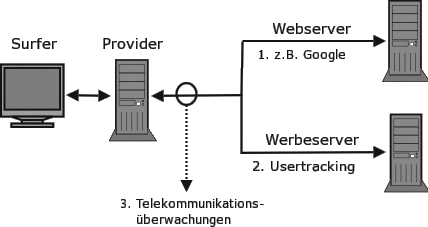
\includegraphics[scale=0.65]{../grafiken/surfen.png}
\caption{M�glichkeiten zur �berwachung im WWW}
\end{center}
\end{figure}

Neben den Big Data Firmen werden auch staatliche Ma�nahmen zur �berwachung derzeit stark ausgebaut und m�ssen von Providern unterst�tzt werden. Nicht immer sind die vorgesehenen Ma�nahmen rechtlich unbedenklich.

\newpage
\section{Big Data - Kunde ist der, der bezahlt}
Viele Nutzer dieser Dienste sehen sich in der Rolle von \textit{Kunden}. Das ist falsch. Kunde ist der, der bezahlt. Kommerzielle Unternehmen (insbesondere b�rsennotierte Unternehmen) optimieren ihre Webangebote, um den zahlenden Kunden zu gefallen und den Gewinn zu maximieren. Die vielen Freibier-Nutzer sind bestenfalls \textit{gl�ckliche Hamster im Laufrad}, die die verkaufte Ware produzieren.

\subsection{Google}
Das Beispiel Google wurde aufgrund der Bekanntheit gew�hlt. Auch andere Firmen geh�ren zu den Big Data Companies und versuchen mit �hnlichen Gesch�ftsmodellen Gewinne zu erzielen. Im Gegensatz zu Facebook, Twitter... usw. verkauft Google die gesammelten Informationen �ber Nutzer nicht an Dritte sondern verwendet sie intern f�r Optimierung der Werbung. Nur an die NSA werden nach Informationen des Whistleblowers W. Binney zuk�nftig Daten weitergegeben.

\subsubsection*{Wirtschaftliche Zahlen}
Google hat einen j�hrlichen Umsatz von 37 Milliarden Dollar, der ca. 9,4 Milliarden Dollar Gewinn abwirft. 90\% des Umsatzes erzielt Google mit personalisierter Werbung. Die Infrastruktur kostet ca. 2 Millarden Dollar j�hrlich. (Stand: 2011)

\subsubsection*{Google Web Search}
Googles Websuche ist in Deutschland die Nummer Eins. 89\% der Suchanfragen gehen direkt an \textit{google.de}. Mit den Suchdiensten wie Ixquick, Metager2, Web.de... die indirekt Anfragen an Google weiterleiten, beantwortet der Primus ca. 95\% der deutschen Suchanfragen. (Stand 2008)

\begin{enumerate}
 \item Laut Einsch�tzung der Electronic Frontier Foundation werden alle Suchanfragen protokolliert und die meisten durch Cookies, IP-Adressen und Informationen von Google Accounts einzelnen Nutzern zugeordnet.\\

In den Datenschutzbestimmungen von Google kann man nachlesen, dass diese Informationen (in anonymisierter Form) auch an Dritte weitergegeben werden. Eine Einwilligung der Nutzer in die Datenweitergabe liegt nach Ansicht der Verantwortlichen vor, da mit der Nutzung des Dienstes auch die AGBs akzeptiert wurden. Sie sind schlie�lich auf der Website �ffentlich einsehbar.

\item Nicht nur die Daten der Nutzer werden analysiert. Jede Suchanfrage und die Reaktionen auf die angezeigten Ergebnisse werden protokolliert und ausgewertet.\\

Google Flu Trends zeigt, wie gut diese Analyse der Suchanfragen bereits arbeitet. Anhand der Such-Protokolle wird eine Ausbreitung der Grippe um 1-2 Wochen schneller erkannt, als es bisher dem  U.S. Center for Disease Control and Prevention m�glich war.\\

Die mathematischen Grundlagen f�r diese Analysen wurden im Rahmen der Bewertung von Googles 20\%-Projekten entwickelt. Bis 2008 konnten Entwickler bei Google 20\% ihrer Arbeitszeit f�r eigene Ideen verwenden. Interessante Ans�tze aus diesem Umfeld gingen als Beta-Version online (z.B. Orkut). Die Reaktionen der Surfer auf diese Angebote wurde genau beobachtet. Projekte wurden wieder abgeschaltet, wenn sie die harten Erfolgskriterien nicht erf�llten (z.B. Google Video).\\

Inzwischen hat Google die 20\%-Klausel abgeschafft. Die Kreativit�t der eigenen Mitarbeiter ist nicht mehr notwendig und zu teuer. Diese �nderung der Firmenpolitik wird von einer Fluktuation des Personals begleitet. 30\% des kreativen Stammpersonals von 2000 haben der Firma inzwischen den R�cken zugekehrt. (Stand 2008)\\

Die entwickelten Bewertungsverfahren werden zur Beobachtung der Trends im Web eingesetzt. Der Primus unter den Suchmaschinen ist damit in der Lage, erfolgversprechende Ideen und Angebote schneller als alle Anderen zu erkennen und darauf zu reagieren. Die Ideen werden nicht mehr selbst entwickelt, sondern aufgekauft und in das Imperium integriert. Seit 2004 wurden 60 Firmen �bernommen, welche zuvor die Basis f�r die meisten aktuellen Angebote von Google entwickelt hatten: Youtube, Google Docs, Google Maps, Google Earth, Google Analytics, Picasa, SketchUp, die Blogger-Plattformen...\\

Das weitere Wachstum des Imperiums scheint langfristig gesichert.\\

Zu sp�t hat die Konkurrenz erkannt, welches enorme Potential die Auswertung von Suchanfragen darstellt. Mit dem B�rsengang 2004 musste Google seine Geheimniskr�merei etwas lockern und f�r die B�senaufsicht Gesch�ftsdaten ver�ffentlichen. Microsoft hat daraufhin Milliaden Dollar in \textit{MSN Live Search, Bing} versenkt und Amazon, ein weiterer Global Player im Web, der verniedlichend als Online Buchh�ndler bezeichnet wird, versuchte mit \textit{A9} ebenfalls eine Suchmaschine zu etablieren.
\end{enumerate}

\subsubsection*{Adsense, DoubleClick, Analytics \& Co.}
Werbung ist die Haupteinnahmequelle von Google. Im dritten Quartal 2010 erwirtschaftete Google 7,3 Milliarden Dollar und damit 97\% der Einnahmen aus Werbung. Zielgenaue Werbung basierend auf umfassenden Informationen �ber Surfer bringt wesentliche h�here Eink�nfte, als einfache Bannerschaltung. Deshalb sammeln Werbetreibende im Netz, umfangreiche Daten �ber Surfer. Es wird beispielsweise verfolgt, welche Webseiten ein Surfer besucht und daraus ein Ineressenprofil abgeleitet. Die Browser werden mit geeigneten Mitteln markiert (Cookies u.�.), um Nutzer leichter wieder zu erkennen.\\

Inzwischen lehnen 84\% der Internetnutzer dieses Behavioral Tracking ab. Von den Unternehmen im Internet wird es aber stetig ausgebaut. Google ist auf diesem Gebiet f�hrend und wird dabei (unwissentlich?) von vielen Website Betreibern unterst�tzt.\\

97\% der TOP100 Websites und ca. 80\% der deutschsprachigen Webangebote sind mit verschiedenen Elementen von Google f�r die Einblendung kontextsensitiver Werbung und Traffic-Analyse infiziert! (Reppesgaard: Das Google Imperium, 2008) Jeder Aufruf einer derart pr�parierten Website wird bei Google registriert, ausgewertet und einem Surfer zugeordnet.\\

Neben kommerziellen Verkaufs-Websites, Informationsangeboten professioneller Journalisten und Online-Redaktionen geh�ren die Websites politischer Parteien genauso dazu, wie unabh�ngige Blogger auf den Plattformen \textit{blogger.com} und \textit{blogspot.com} sowie private Websites, die sich �ber ein paar Groschen aus dem Adsense-Werbe-Programm freuen.\\

Untragbar wird diese Datenspionage, wenn politische Parteien wie die CSU ihre Spender �berwachen lassen. Die CSU bietet ausschlie�lich die M�glichkeit, via Paypal zu spenden. Die Daten stehen damit inklusive Wohnanschrift und Kontonummer einem amerikanischen Gro�unternehmen zur Verf�gung. Au�erdem l�sst die CSU ihre Spender mit Google-Analytics beobachten. Der Datenkrake erh�lt damit eindeutige Informationen �ber politischen Anschauungen. Diese Details k�nnen im Informationskrieg wichtig sein.\\

Damit kennt das Imperium nicht nur den Inhalt der Websites, die vom Google-Bot f�r den Index der Suchmaschine abgeklappert wurden. Auch Traffic und Besucher der meisten Websites sind bekannt. Diese Daten werden Werbetreibenden anonymisiert zur Verf�gung gestellt.\\

\begin{figure}[htb]
\begin{center}
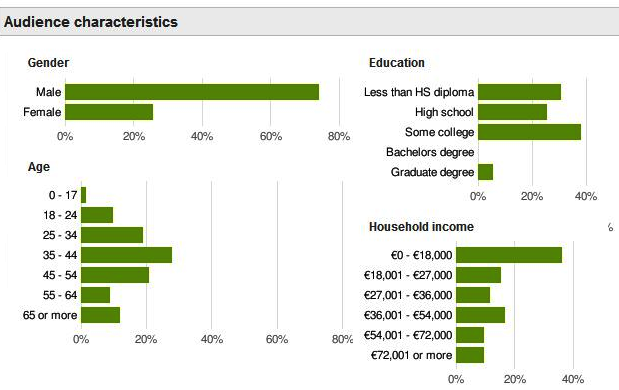
\includegraphics[scale=0.65]{../screenshots/ad-planner.png}
\caption{Ad-Planner Besucherstatistik (Beispiel)}
\label{abb:adplanner1}
\end{center}
\end{figure}

Die Grafik Bild \ref{abb:adplanner1} zur Besucherstatistik wurde vom Google Ad-Planner f�r eine (hier nicht genannte) Website erstellt. Man erkennt, das der �berwiegende Anteil der Besucher m�nnlich und zwischen 35-44 Jahre alt ist. (Die Informationen zu Bildung und Haushaltseinkommen m�ssen im Vergleich zu allgm. Statistiken der Bev�lkerung bewertet werden, was hier mal entf�llt.)\\

\textbf{Wie kommt das Imperium zu diesen Daten?} Es gibt so gut wie keine M�glichheit, diese Daten irgendwo einzugeben. Google fragt NICHT nach diesen Daten, sie werden aus der Analyse des Surf- und Suchverhaltens gewonnen. Zus�tzlich kauft Google bei Marktforschungsunternehmen gro�e Mengen an Informationen, die in die Kalkulation einflie�en.\\

Wenn jemand mit dem iPhone auf der Website von BMW die Preise von Neuwagen studiert, kann Google ihn einer Einkommensgruppe zuordnen. Wird der Surfer sp�ter beim Besuch von Spiegel-Online durch Einblendung von Werbung wiedererkannt, kommt ein entsprechender Vermerk in die Datenbank. Au�erdem kann die Werbung passend zu seinen Interessen und Finanzen pr�sentiert werden. (Die Realit�t ist nat�rlich etwas komplexer.)\\

Mit dem im April 2010 eingef�hrtem \textbf{Retargeting} geht Google noch weiter. Mit Hilfe spezieller Cookies werden detailierte Informationen �ber Surfer gesammelt. Die Informationen sollen sehr genau sein, bis hin zu Bekleidungsgr��en, f�r die man sich in einem Webshop interessiert hat. Die gesammelten Informationen sollen die Basis f�r punktgenaue Werbung bieten. Beispielsweise soll nach dem Besuch eines Webshops f�r Bekleidung ohne Kaufabschluss permanent alternative Werbung zu diesem Thema eingeblendet werden. 

\subsubsection*{Google Mail, Talk, News... und Google+ (personalisierte Dienste)}
Mit einem einheitlichem Google-Konto k�nnen verschiedene personalisierte Angebote genutzt werden. (Google Mail, News, Talk, Calendar, Alert, Orkut, B�rsennachrichten..... iGoogle)\\

Bei der Anmeldung ist das Imperium weniger wissbegierig, als vergleichbare kommerzielle Anbieter. Vor- und Nachname, Login-Name und Passwort reichen aus. Es ist nicht unbedingt n�tig, seinen realen Namen anzugeben. Ein Pseudonym wird auch akzeptiert. Die Accounts erm�glichen es, aus dem Surf- und Suchverhalten, den zusammengestellten Nachrichtenquellen, dem Inhalt der E-Mails usw. ein Profil zu erstellen. Die unsicher Zuordnung �ber Cookies, IP-Adressen und andere Merkmale ist nicht n�tig. Au�erdem dienen die Dienste als Fl�chen f�r personalisierte und gut bezahlte Werbung.\\

Patente aus dem Umfeld von Google Mail zeigen, dass dabei nicht nur Profile �ber die Inhaber der Accounts erstellt werden, sondern auch die Kommunikationspartner unter die Lupe genommen werden. Wer an einen Google Mail Account eine E-Mail sendet, landet in der Falle des Datenkraken.\\

Die Einrichtung eines Google-Accounts erm�glicht es aber auch, gezielt die gesammelten Daten in gewissem Umfang zu beeinflussen. Man kann Eintr�ge aus der Such- und Surf-Historie l�schen u.�. (Besser ist es sicher, die Eintr�ge von vornherein zu vermeiden.)

\subsubsection*{Smartphones und Android}
2005 hat Google die Firma Android Inc. f�r 50 Mio. Dollar gekauft sucht mit dem Smartphone Betreibssystem Android auf dem Markt der mobilen Kommunikation �hnliche Erfolge wie im Web.\\

Das erste Google Handy \textit{G1} war ein in Hardware gegossenes Pendant zum Webbrowser Google Chrome. Bei der Markteinf�hr�hrung versuchte Google die Nutzer mit dem ersten Einschalten zu �berreden, einen Google-Account anzulegen. Ohne Account bei Google ging fast nichts mit dem Hightech-Spielzeug, nur Telefonieren war m�glich. Dieses Feature wurde auf Druck der Nutzer deaktiviert.\\

Bei der Nutzung von Android Smartphones sollen alle E-Mails �ber Google Mail laufen, Termine mit dem Google Calendar abgeglichen werden, die Kontaktdaten sollen bei Google landen\dots Die Standortdaten werden st�ndig an Google �bertragen, um sogenannte Mehrwertdienste bereit zu stellen (genau wie das iPhone die Standortdaten an Apple sendet).\\

Inzwischen ist die feste Bindung an Google-Dienste unter Android etwas gelockert. Aber nach wie vor sind diese als Standard voreingestellt und werden aus Bequemlichkeit sicher von der Mehrzahl der Nutzer verwendet.

\subsubsection*{Mozilla Firefox}
Google ist der Hauptsponsor der Firefox Entwickler. Seit 2012 zahlt Google j�hrlich 300 Mio. Dollar an die Mozilla Foundation, um die voreingestellte Standardsuchmaschine in diesem Browser zu sein.\\

Das ist nat�rlich in erster Linie ein Angriff auf Microsoft. Die Entwickler von Firefox kommen ihrem datensammelden Hauptsponsor jedoch in vielen Punkten deutlich entgegen:
\begin{itemize}
 \item Google ist die einzige allgemeine Suchmaschine, die unbedarften Nutzern zur Verf�gung steht. Alternativen sind standardm��ig nicht vorhanden und m�ssen von den Nutzer aktiv gesucht und installiert werden.
\item Die Default-Startseite erm�glicht es Google, ein langlebiges Cookie zu setzen und den Browser damit praktisch zu personalisieren.
\item Sollte die Startseite modifiziert werden (z.B. bei der Variante \textit{Iceweasel} von Debian GNU/Linux), erfolgt die ``Personalisierung'' des Browsers wenige Minuten sp�ter durch Aktualisierung der Phishing-Datenbank.
\item Diese ``Personalisierung'' erm�glicht es Google, den Nutzer auf allen Webseiten zu erkennen, die mit Werbeanzeigen aus dem Imperium oder Google-Analytics verschmutzt sind. Im deutschsprachigen Web hat sich diese Verschmutzung auf 4/5 der relevanten Webseiten ausgebreitet.
\end{itemize}
(Trotzdem ist Mozilla Firefox ein guter Browser. Mit wenigen Anpassungen und Erweiterungen von unabh�ngigen Entwicklern kann man ihm die Macken austreiben und spurenarm durchs Web surfen.)

\subsubsection*{Google DNS}
Mit dem DNS-Service versucht Google, die Digital Natives zu erreichen, Surfer die in der Lage sind, Cookies zu blockieren, Werbung auszublenden und die nat�rlich einen DNS-Server konfigurieren k�nnen.\\

Google verspricht, dass die DNS-Server unter den IP-Adressen 8.8.8.8 und 8.8.4.4 nicht kompromittiert oder zensiert werden und bem�ht sich erfolgreiche um schnelle DNS-Antworten. Die Google-Server sind etwa 1/10 sec bis 1/100 sec schneller als andere unzensierte DNS-Server.\\

Nat�rlich werden alle Anfragen gespeichert und ausgewertet. Ziel ist, die von erfahrenen Nutzern besuchten Websites zu erfassen und in das Monitoring des Web besser einzubeziehen. Positiv an dieser Initiative von ist, dass es sich kaum jemand leisten kann, die Wirtschaftsmacht Google zu blockieren. Damit wird auch die Sperrung alternativer DNS-Server, wie es in Deutschland im Rahmen der Einf�hrung der Zensur geplant war, etwas erschwert.

\subsubsection*{Kooperation mit Beh�rden und Geheimdiensten}
Es w�re verwunderlich, wenn die gesammelten Datenbest�nde nicht das Interesse der Beh�rden und Geheimdienste wecken w�rden. Google kooperiert auf zwei Ebenen:
\begin{enumerate}
 \item 
       
Auf Anfrage stellt Google den Beh�rden der L�nder die angeforderten Daten zur Verf�gung. Dabei agiert Google auf Grundlage der nationalen Gesetze. Bei daten-speicherung.de findet man Zahlen zur Kooperationswilligkeit des Imperiums. Durchschnittlich beantwortet Google Anfragen mit folgender H�ufigkeit:
\begin{itemize}
\item 3mal t�glich von deutschen Stellen
\item 20mal t�glich von US-amerikanischen Stellen
\item 6mal t�glich von britischen Stellen
\end{itemize}
\item Au�erdem kooperiert Google mit der CIA bei der Auswertung der Datenbest�nde im Rahmen des Projektes \textit{Future of Web Monitoring}, um Trends und Gruppen zu erkennen und f�r die Geheimdienste der USA zu erschlie�en. Es besteht der Verdacht, dass Google auch mit der NSA kooperiert. Das EPIC bem�ht sich, Licht in diese Kooperation zu bringen. Anfragen wurden bisher nicht beantwortet. Nach Inforamtionen des Whistleblowsers W. Binney, der 30 Jahre in f�hrenden Positionen der NSA gearbeitet hat, wird Google ab Herbst 2012 Kopien des gesamten E-Mail Verkehrs von GMail und s�mtliche Suchanfragen dem neuen Datacenter der NSA in Bluffdale zur Verf�gung stellen.
\begin{quote}
 \textit{It will store all Google search queries, e-mail and fax traffic and so on.}
\end{quote} 
\end{enumerate}

\subsubsection*{Die (virtuelle) Welt ist eine ``Google'' - oder?}
Die vernetzten Rechenzentren von Google bilden den mit Abstand gr��ten Supercomputer der Welt. Dieser Superrechner taucht in keiner TOP500-Liste auf, es gibt kaum Daten, da das Imperium sich bem�ht, diese Informationen geheim zu halten. Die Datenzentren werden von (selbst�ndigen?) Gesellschaften wie Exaflop LLC betrieben.\\

Neugierige Journalisten, Blogger und Technologieanalysten tragen laufend neues Material �ber diese Maschine zusammen. In den Materialsammlungen findet man 12 bedeutende Anlagen in den USA und 5 in Europa, die als wesentliche Knotenpunkte des Datenuniversums eingesch�tzt werden. Weitere kleinere Rechenzentren stehen in Dublin, Paris, Mailand, Berlin, M�nchen Frankfurt und Z�rich. In Council Bluffs (USA), Thailand, Malaisia und Litauen werden neue Rechenzentren gebaut, die dem Imperium zuzurechnen sind. Das gr��te aktuelle Bauprojekt vermuten Journalisten in Indien. (2008)\\

Experten sch�tzen, dass ca. 1 Mio. PCs in den Rechenzentren f�r Google laufen (Stand 2007). Alle drei Monate kommen etwa 100 000 weitere PCs hinzu. Es werden billige Standard-Komponenten verwendet, die zu Clustern zusammengefasst und global mit dem \textit{Google File System (GFS)} vernetzt werden. Das GFS gew�hrleistet dreifache Redundanz bei der Datenspeicherung.\\

Die Kosten f�r diese Infrastruktur belaufen sich auf mehr als zwei Milliarden Dollar j�hrlich. (2007)\\

Die Videos von Youtube sollen f�r 10\% des gesamten Traffics im Internet verantwortlich sein. �ber den Anteil aller Dienste des Imperiums am Internet-Traffic kann man nur spekulieren.
\begin{center}
\textbf{Google dominiert unser (virtuelles) Leben.}                                          \end{center}
Dabei geht es nicht um ein paar Cookies sondern um eine riesige Maschinerie.

\subsection{Datenh�ndler}
Die Datensammler (Facebook, Amazon, Twitter...) verkaufen Informationen �ber Nutzer an Daten�h�ndler (z.B. Acxiom, KaiBlue, RapLeaf...), welche die Daten anreichern, zusammen�fassen und umfassende Profile den eigentlichen Endnutzern wie Kreditkartenfirmen, Personal�abteilungen gro�er Unternehmen und Marketingabteilungen von Mikrosoft bis Blockbuster verkaufen.

\begin{description}
\item[Acxiom] konnte bereits 2001, noch bevor Facebook als Datenquelle zur Verf�gung stand, auf umfangreiche Datenbest�nde verweisen. Als das FBI die Namen der angeblichen 9/11 Attent�ter ver�ffentlichte (von denen noch heute einige quicklebendig sind), lieferte Acxiom mehr Daten zu diesen Personen, als alle Geheimdienste zusammen - inklusive fr�herer und aktueller Adressen, Namen der Mitbewohner usw. Im Rahmen der Zusammenarbeit mit FBI und CIA f�hrten die Daten von Acxiom mehrfach zu Anklagen und Abschiebungen (nach Ausage eines leitenden Mitarbeiters).\\

 Acxiom protzt damit, pr�zise Daten �ber 96\% der amerikanischen Bev�lkerung zu haben. Jeder Datensatz hat 1.500 Datenpunkte (Stand 2010). Neben Daten zur Internetnutzung ver�arbeitet Acxiom auch Kreditkartenrechnungen, Apothekenrechnungen und andere Daten aus der realen Welt.
\begin{quote}
\textit{Sie k�nnen sich Acxiom wie eine automatisierte Fabrik vorstellen, wobei das Produkt, das wir herstellen, Daten sind.} (Aussage eines Technikers von Acxiom)
\end{quote} 

\item[RapLeaf] wurde von P. Thiel gegr�ndet, der auch die Gr�ndung von PayPal.com finanzierte, bei Facebook ma�geblichen Einfluss hat und dessen Credo eine totale Personalisierung des Internet ist.\\

RapLeaf sammelt selbst Daten �ber die Internetnutzung, verarbeitet aber auch hinzu�gekaufte Daten. Die Informationen werden anhand von E-Mail Adressen zusammen�gefasst. Jeder kann auf der Website eine Liste von E-Mail Adressen hochladen, bezahlen und nach Zahlungseingang die Daten abrufen. Ein kleiner Auszug aus der Preisliste (Stand 2011) soll den Wert pers�nlicher Informationen zeigen:
\begin{itemize}
 \item Alter, Geschlecht und Ort: 0 Cent (Lockangebot)
 \item Haushaltseinkommen: 1 Cent pro E-Mail-Adresse
 \item Ehestand: 1 Cent pro E-Mail-Adresse
 \item vorhandene Kinder: 1 Cent pro E-Mail-Adresse
 \item Wert des bewohnten Hauses: 1 Cent pro E-Mail-Adresse
 \item Relation von Krediten zum Verm�gen: 1 Cent pro E-Mail-Adresse
 \item vorhandene Kreditkarten: 1 Cent pro E-Mail-Adresse
 \item Fahrzeuge im Haushalt: 1 Cent pro E-Mail-Adresse
 \item Smartphone Nutzung: 3 Cent pro E-Mail-Adresse
 \item Beruf und Ausbildung: 2 Cent pro E-Mail-Adresse
 \item T�tigkeit als Blogger: 3 Cent pro E-Mail-Adresse
 \item wohlt�tige Spenden: 3 Cent pro E-Mail-Adresse
 \item Pr�ferenzen f�r hochwertige Marken: 3 Cent pro E-Mail-Adresse
 \item Pr�ferenzen f�r B�cher, Zeitschriften: 3 Cent pro E-Mail-Adresse
 \item \dots
\end{itemize}
Eine Analyse des Wall Street Journal hat sich n�her mit den Datensammlungen Firma besch�ftigt \footnote{ \href{http://online.wsj.com/article/SB10001424052748703940904575395073512989404.html}{http://online.wsj.com/article/SB10001424052748703940904575395073512989404.html}}.
 \end{description}

\section{Techniken der Datensammler}
Viele Dienste im Web nutzen die M�glichkeiten, das Surfverhalten zu verfolgen, zu analysieren und die gesammelten Daten zu versilbern. Die dabei entstehenden Nutzerprofile sind inzwischen sehr aussagekr�ftig. Wie das Wall Street Journal in einer Analyse beschreibt, k�nnen das Einkommen, Alter, politische Orientierung und weitere pers�nliche Daten der Surfer eingesch�tzt werden oder die Wahrscheinlichkeit einer Kreditr�ckzahlung. Haupts�chlich werden diese Daten f�r Werbung genutzt. Ein Online-Versand von Brautkleidern m�chte Frauen im Alter von 24-30 Jahren ansprechen, die verlobt sind. Das ist heute m�glich.\\

Es geht aber l�ngst nicht nur um die Einblendung von Werbung. Sarah Downey warnt \footnote{ \href{http://heise.de/-1628313}{http://heise.de/-1628313}} vor wachsenden realen Sch�den durch das Online-Tracking. Die gesammelten Informationen k�nnen den Abschluss von Versicherungen und Arbeitsvertr�gen beeinflussen oder sie k�nnen zur Preisdiskriminierung genutzt werden. Ganz einfaches Beispiel: das US-Reiseportal Orbitz bietet z.B. Surfern mit MacOS Hotelzimmer an, die 20-30 Dollar teuerer sind, als die Zimmer der Windows Nutzern angeboten werden.\footnote{ \href{http://heise.de/-1626368}{http://heise.de/-1626368}}.\\

\subsubsection*{Techniken zum Tracking des Surfverhaltens}
Das Surfverhalten liefert die meisten Informationen �ber unsere Vorlieben. Dabei werden folgende Techniken eingesetzt:
\begin{description}
 \item[Cookies] sind noch immer das am h�ufigsten eingesetzte Mittel, um Surfer zu markieren und �ber mehrere Webseiten zu verfolgen.
 \item[Flash-Cookies] werden seit 2005 verwendet, um gel�schte Tracking-Cookies wieder�herzu�stellen. Sie sind unabh�ngig vom Browser und funktionieren auch, wenn man verschiedene Browser oder Browserprofile f�r spurenarmes Surfen und Fun-Surfen nutzt.
 \item[HTML-Wanzen] (sogenannte Webbugs) sind 1x1-Pixel gro�e transparente Bildchen, die in den HTML-Code einer Webseite eingebettet werden. Sie sind f�r den Nutzer unsichtbar. Beim Laden einer Webseite werden sie von einem externen Server geladen und hinter�lassen Eintr�ge in den Logdaten. Au�erdem k�nnen sie Cookies transportieren.
 \item[EverCookies] nutzen moderne HTML5 Techniken wie DomStorage, ETags aus dem Cache und andere Techniken, um den Surfer zu markieren und sp�ter anhand dieser Markierungen wiederzuerkennen. Der polnische Informatiker Samy Kamkar hat eine Web�seite zur Demonstration von EverCookie Techniken\footnote{ \href{http://samy.pl/evercookie/}{http://samy.pl/evercookie}} erarbeitet. 38\% der popul�ren Web�seiten nutzen bereits verschiedene EverCookie Techniken (Stand: Okt. 2012).
 \item[Browser Fingerprinting] nutzt verschiedene Merkmale des Browsers wie z.B. Browser�version, installierte Schriftarten, Bildschirmgr��e, bevorzugte Sprachen und weitere mit Javascript auslesbare Daten, um einen Fingerprint zu berechnet. Dieser Fingerprint ist f�r viele Surfer eindeutig. Das Projekt Panopticlick der EFF.org zeigte, dass mehr als 80\% der Surfer damit eindeutig erkennbar sind. Die Erkennungsrate stieg auf 94\%, wenn Flash- oder Java-Applets zus�tzlich genutzt werden konnten. Die Firma Bluecava nutzt ausschlie�lich Browser Fingerprinting und protzt mit 30\% besseren Ergebnissen als Cookie-basierte Techniken\footnote{ \href{http://www.bluecava.com/visitor-insight-campaign-measurement}{http://www.bluecava.com/visitor-insight-campaign-measurement}}. Andere Trackingfirmen (z.B. Google, Multicounter) nutzen diese Informationen zus�tzlich, um die Erkennungsraten zu verbessern \footnote{ \href{http://www.multicounter.de/features.html}{http://www.multicounter.de/features.html}}.
\end{description}

Die Tracking-Elemente k�nnen in die Webseiten eingebettet werden (First-Party Content) oder sie k�nnen von externen Servern nachgeladen werden (Third-Party Content). Au�erdem werden sie durch Einblendungen von Werbebanner transportiert oder durch die Like-Buttons der Social Networks.\\

F�r die Auswertung werden nicht nur die Informationen zur besuchten Webseite genutzt. Besonders aussagekr�ftig sind die Klicks auf Werbung. S. Guha von Microsoft und B. Cheng sowie P. Francis vom Max-Planck-Institut f�r Software Systeme habe ein Paper ver�ffentlicht, wie man homosexuelle M�nner anhand der Klicks auf Werbung erkennen kann\footnote{ \href{http://arstechnica.com/tech-policy/news/2010/10/more-privacy-headaches-for-facebook-gay-users-outed-to-advertisers.ars}{http://arstechnica.com/tech-policy/news/2010/10/more-privacy-headaches-for-facebook-gay-users-outed-to-advertisers.ars}}. Das Verfahren kann f�r verschiedene Fragestellungen angepasst werden. Die Klicks auf Facebook Like Buttons k�nnen in der gleichen Weise ausgewertet werden. Forscher der Universit�t Cambridge (Gro�britannien) konnten bei einer Untersuchung die sexuelle Orientierung und politische Einstellung der Nutzer anhand der Klicks auf Like Buttons vorhersagen\footnote{ \href{http://heise.de/-1820638}{http://heise.de/-1820638}}. Damit 
verr�t man m�glicherweise mehr private Informationen, als man eigentlich ver�ffentlichen m�chte.

\subsubsection*{Tracking von E-Mail Newslettern}
Die Markierung von E-Mail Newslettern ist weit verbreitet. Es geht dabei darum, das �ffnen der E-Mails zu beobachten und die Klicks auf Links in den Newslettern zu verfolgen.
\begin{itemize}
 \item Wie beim Tracking des Surfverhaltens werden kleine 1x1 Pixel gro�e Bildchen in die E-Mail eingebettet, die beim Lesen im HTML-Format von einem externen Server geladen werden. Durch eine indivuelle, nutzerspezifische URL kann die Wanze eindeutig einer E-Mail Adresse zugeordnet werden. Ein Beispiel aus dem E-Mail Newsletter von Paysafecard, das einen externen Trackingservice nutzt:
\begin{verbatim}
   <IMG src="http://links.mkt3907.com/open/log/43.../1/0">
\end{verbatim} 
Easyjet.com (ein Billigflieger) kann offenbar die Aufrufe seiner Newsletter selbst z�hlen und auswerten. In den E-Mails mit Informationen zu gebuchten Fl�gen findet man folgende kleine Wanze am Ende der Mail:
\begin{verbatim}
   <IMG src="http://mail.easyjet.com/log/bEAS001/mH9..."
        height=0 width=0 border=0>
\end{verbatim}
Bei kommerziellen E-Mail Newslettern kann man fast sicher davon ausgehen, dass sie Wanzen enthalten. Ich habe diese Trackingelemente in so gut wie allen kommerziellen Newslettern von \textit{PayPal.com, Easyjet, AirBerlin, Paysafe�card, UKash} usw. gefunden. Einzige Ausnahme war bisher die Firma Softmaker. Es wird aber nicht nur im kommerziellen Bereich verwendet. Die CDU Brandenburg markierte ihre Newsletter �ber einen l�ngeren Zeitraum, um zu �berpr�fen, wann und wo sie gelesen wurden. \textit{ACCESS Now} und \textit{Abgeordnetenwatch} sind weitere Bespiele.
\item Die Links in den E-Mails f�hren oft nicht direkt zum Ziel. Sie werden �ber einen Tracking�service geleitet, der jeden Klick individuell f�r jede Empf�nger�adresse protokolliert und danach zur richtigen Seite weiterleitet. Als Bespiel soll ein Link aus dem Paysafe�card Newsletter dienen, der zu einem Gewinn�spiel auf der Paysafecard Webseite f�hren soll:
\begin{verbatim}
   <a href="http://links.mkt3907.com/ctt?kn=28&ms=3N...">
   Gewinne Preise im Wert von 10.000 Euro</a>
\end{verbatim} 
\end{itemize}



\subsubsection*{Tracking von Dokumenten (PDF, Word usw.)}
Die Firma ReadNotify bietet einen Service, der Word-Dokumente und PDF-Dateien mit speziellen unsichtbaren Elementen versieht. Diese werden beim �ffnen des Dokumentes vom Server der Firma nachgeladen und erlauben somit eine Kontrolle, wer wann welches Dokument �ffnet. Via Geo-Location ermittelt ReadNotify auch den ungef�hren Standort des Lesers.\\




\subsubsection*{Tendenzen beim Tracking des Surfverhaltens}
Obwohl 80\% der Internetnutzer das Tracking des Surfverhaltens ablehnen, wird es stetig weiter ausgebaut. Dabei sind folgende Tendenzen erkennbar:
\begin{enumerate}
 \item Mehr Trackingelemente werden auf den Webseiten eingesetzt. Das Projekt Web Privacy Census der University of California verfolgt seit mehreren Jahren die Entwicklung und dokumentiert einen stetigen Anstieg von Trackingelementen bei den meistbesuchten Webseiten (Top-100, Top-1000 und Top-25.000). Als Beispiel soll die Anzahl der Cookies dienen, die beim Besuch der 100 popul�rsten Webseiten gesetzt werden (ohne Login, nur beim Betrachten der Webseiten):
 \begin{center}
 \begin{tabular}{c|c}
& Anzahl der Cookies\\
 \hline
2009 & 3.602\\
2011 & 5.675\\
2012 & 6.485
\end{tabular}
\end{center}
84\% der Cookies stammen dabei von Drittseiten. Die Daten werden an mehr als 600 Server �bertragen.

\item Das Projekt registriert eine �berproprtionale Zunahme schwer blockierbarer Trackingfeatures (EverCookies). Immer mehr Webseiten verwenden HTML5 DomStorage, IE\_userdata oder ETags aus dem Cache f�r die Verfolgung des Surfverhaltens. F�r die meistbesuchten Webseiten wurden folgende Zahlen zur Nutzung von EverCookies ermittelt:
\begin{center}
 \begin{tabular}{c|c}
& Nutzung von EverCookies\\
 \hline
2011 & 19\% der Webseiten\\
2012 (Mai) & 34\% der Webseiten\\
2012 (Okt.) & 38\% der Webseiten
\end{tabular}
\end{center}

\item Flash-Cookies (LSOs) werden seltener eingesetzt. Diese Technik befindet sich auf dem absteigenden Ast. Im Oktober 2012 setzten nur noch 11\% der popul�ren Webseiten Flash-Cookies ein. Dabei handelt es sich �berwiegend um Webseiten mit Flash-Videos. \textit{Youporn.com} speichert pers�nliche Preferenzen beispielsweise in Flash-Cookies.

\item Durch den Aufkauf kleinerer Anbieter durch die Gro�en der Branche erfolgt eine Markt�bereinigung. Es bilden sich sogenannte Tracking-Familien, die die Daten untereinander austauschen und somit eine gro�e Reichweite bei der Beobachtung des Surfverhaltens haben. Die gr��ten Tracking-Familien sind:
\begin{enumerate}
 \item Die Google-Familie ist unangefochten die Nummer Eins. 44\% der weltweiten Ums�tze in der Onlinewerbung werden durch diese Gruppe erzielt. Das Google Imperium hat in den letzten Jahren die Firmen \textit{YouTube, DoubleClick mit falkad.net, FeedBurner, Springs, Adscape, AdMob, Teracent, Invite Media, Admeld, Adelphic, Wildfire Interactive} u.a.m. aufgekauft. Die folgende Tabelle zeigt, wie das Google Imperium dadurch seine Pr�senz auf den 1000 popul�rsten Webseiten in den letzten Jahren ausbauen konnte:
\begin{center}
 \begin{tabular}{c|c}
& Trackingelemente der Google-Familie\\
 \hline
2005 & auf 7\% der Webseiten\\
2006 & auf 16\% der Webseiten\\
2008 & auf 55\% der Webseiten\\
2009 & auf 80\% der Webseiten\\
2012 & auf 97\% der Webseiten\\
\end{tabular}
\end{center}

 \item Auf den Pl�tzen 2-4 folgen die Tracking-Familien von Microsoft (u.a. mit den Trackingdiensten \textit{atdmt.com, adbureau.com, aquantive.com}), die 
 Yahoo! Familie (mit den Trackingdiensten \textit{adrevolver, yieldmanager, overture}) und die AOL-Familie (mit \textit{adsonar.com, tacoda.net, advertising.com}) mit einem Marktanteil von jeweils 3-8\%.
 \item Die im Februar 2013 vereinbarten Kooperation von Facebook mit den bisher eigen�st�ndigen Tracking�diensten BlueKai und Epsilon bildet den Kern einer neuen bedeutenden Tracking Familie.
\end{enumerate}


\item Die Beobachtung des Surfverhaltens und der Online-Eink�ufe liefert nur ein unvollst�ndiges Bild unserer Interessen. Durch Einbeziehung von Daten aus dem realen Leben sollen die Profile verbessert werden.
\begin{itemize}
 \item Im Februar 2013 hat Facebook eine Kooperation mit den Datenh�ndlern \textit{Axciom} und \textit{Datalogix} bekannt gegeben. Diese Firmen werten umfangreiche Daten aus der realen Welt aus (Kredit�kartenzahlungen, Rabatt�karten usw.). Damit sollen die Werbeeinblendung bei Facebook individueller und zielgerichteter auf die Interessen der Mitglieder zugeschnitten werden.
 \item PayPal.com will sein Bezahlsystem auch offline in der realen Welt anbieten und verspricht den teil�nehmenden Gesch�ften, dass sie mehr �ber die Vorlieben ihrer Kunden erfahren werden. Nat�rlich wird auch PayPal.com mehr �ber die realen Interessen der Kunden erfahren.
\end{itemize}



\item Alle Datensammlungen wecken nat�rlich Begehrlichkeiten bei den Geheimdiensten und Strafverfolgern. Leider ist wenig konkretes dar�ber bekannt. Bei der Anh�rung des US Senate Commerce Committee zu den Probleme von Online-Tracking im Juni 2012 sagte B. Liodice als Vertreter der Werbeindustrie, dass das Tracking das Surfverhaltens der Internetnutzer f�r die Sicherheit der USA wichtig und notwendig ist.\\

Die EFF.org kommentierte:
\begin{quote}
 \textit{In yesterday's Senate hearing, we heard the advertising industry admit that their near-ubiquitous online tracking program is being used for issues that are the purview of law enforcement.}
\end{quote} 
\end{enumerate}


\section{Geotagging}
Geotagging ist \textit{the next big thing} unter den Angriffen auf die Privatsph�re. Es geht um die Frage, wo wir etwas tun oder getan haben und welche Bewegungsmuster erkennbar sind. 
\begin{enumerate}
 \item \textbf{Standortdaten} sind die wertvollsten Informationen f�r die Werbe�wirtschaft, um zuk�nftig den Markt zu vergr��ern. Ein Online-Versand von Brautkleidern richtet seine Werbung an Frauen zwischen 24-30 Jahren, die verlobt sind. Ein Ladengesch�ft stellt zus�tzlich die Bedingung, das sie sich h�ufig im Umkreis von xx aufhalten. Lokalisierte Werbung ist ein Markt, der durch die Verbreitung von Smartphones stark w�chst.
\item Die \textbf{Bewegungsanalyse} erm�glicht Aussagen �ber sehr private Details. Man kann z.B. durch die Analyse der Handybewegungen erkennen, ob jemand als Gesch�ftsreisender h�ufig unterwegs ist, ob man ein festes Arbeitsverh�ltnis hat, f�r welche Firma man t�tig ist oder ob man arbeitslos ist. Die Firma Sense Networks ist ein Vorreiter auf dem Gebiet der Bewegungsanalyse. Im Interview mit \textit{Technology Review} beschreibt Greg Skibiski seine Vision:
\begin{quote}
\textit{Es entsteht ein fast vollst�ndiges Modell. Mit der Beobachtung dieser Signale kann man ganze Firmen, ganze St�dte, eine ganze Gesellschaft r�ntgen \footnote{ \href{http://www.heise.de/tr/artikel/Immer-im-Visier-276659.html}{http://www.heise.de/tr/artikel/Immer-im-Visier-276659.html}}.}
\end{quote}

Das Magazin Wired berichtete im Danger Room (Oktober 2011), dass das FBI Smartphones bereits seit Jahren mit der Zielstellung der ``Durchleuchtung der Gesellschaft`` trackt. Muslimisch Communities werden systematisch analysiert, ohne dass die betroffenen Personen im Verdacht einer Straftat stehen. Das Geotracking von GPS-f�higen Smartphones und GPS-Modulen moderner Fahrzeuge durch das FBI erfolgt ohne richterlichen Beschluss.
\begin{quote}
  \textit{\dots the pushpins on the new FBI geo-maps indicate where people live, work, pray, eat and shop, not necessarily where they commit or plan crimes \footnote{ \href{http://www.wired.com/dangerroom/2011/10/fbi-geomaps-muslims/}{http://www.wired.com/dangerroom/2011/10/fbi-geomaps-muslims}}.}
\end{quote} 

\end{enumerate}

 Die Daten werden mit verschiedenen Methoden gesammelt: 
\begin{itemize}
\item Hauptlieferanten f�r Geodaten sind Smartphones und Handys. Vor allem Apps k�nnen genutzt werden, um Geodaten zu sammeln. �ber die H�lfte der in verschiedenen Stores downloadbaren Apps versenden Stand�ortdaten unabh�ngig davon, ob sie f�r die Funktion der App n�tig sind. Der Bundes�daten�schutz�beauftragte erw�hnt beispiels�weise eine App, die das Smartphone zur Taschenlampe macht und dabei den Standort an den Entwickler der App sendet.\\

\item Mit Einf�hrung des iPhone 4 hat Apple seine Datenschutzbestimmungen ge�ndert. Die gesamte Produktpalette von Apple (iPhone, Laptops, PC\dots) wird in Zukunft den Standort des Nutzers laufend an Apple senden. Apple wird diese Daten Dritten zur Verf�gung stellen. Wer Zugang zu diesen Daten hat, wird nicht n�her spezifiziert \footnote{ \href{http://www.apple.com/chde/legal/privacy/}{http://www.apple.com/chde/legal/privacy/}}.\\

F�r die Datensammlungen rund um das iPhone wurde Apple mit dem BigBrother Award 2011 geehrt. Auszug aus der Laudation von F. Rosengart und A. Bogk:
\begin{quote}
\textit{Apples Firmenstrategie scheint darauf ausgelegt zu sein, m�glichst viele Daten der Nutzer zu erfassen, �hnlich wie es soziale Netzwerke auch tun. Werbepartner freuen sich darauf, mit Hilfe von Apple m�glichst zielgruppengerechte und standortbezogene Werbung auf dem Telefon anzeigen zu k�nnen.}
\end{quote} 

\item Millionen von Fotos werden �ber verschiedene Dienste im Internet ver�ffentlicht (Flickr, Twitter, Facebook\dots). H�ufig enthalten diese Fotos in den EXIF-Attributen die GPS-Koordinaten der Aufnahme. Die Auswertung dieses Datenstromes steht erst am Anfang der Entwicklung. Ein Beispiel ist die mit Risikokapital ausgestattete Firma Heypic, die Fotos von Twitter durchsucht und auf einer Karte darstellt.

\item Die ganz normale HTTP-Kommunikation liefert Standortinformationen anhand der IP-Adresse. Aktuelle Browser bieten zus�tzlich eine Geolocation-API, die genauere Informationen zur Verf�gung stellt. Als Facebook im Sommer 2010 die Funktion Places standardm��ig aktivierte, waren viele Nutzer �berrascht, wie genau jede reale Bewegung im Sozialen Netz lokalisiert wird. (Nicht nur Facebook kann das.)\\

\begin{figure}[htb]
\begin{center}
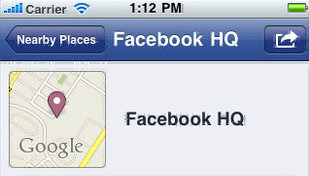
\includegraphics[scale=0.55]{../screenshots/facebook1.png}
\caption{Lokalisierung eines Smartphone durch Facebook}
\label{abb:facebook1}
\end{center}
\end{figure}

Die Deaktivierung von Places scheint bei Facebook wirklich umst�ndlich zu sein. Damit wird aber nicht die Erfassung der Daten deaktiviert, sondern nur die Sichtbarkeit f�r andere Nutzer!

\item Lokalisierungsdienste wie \textit{Gowalla} oder \textit{Foursquare} bieten �ffentlich einsehbare Standortdaten und versuchen, durch spielartigen Charakter neue Nutzer zu gewinnen. Im Gegensatz zu den oben genannten Datensammlungen kann man bei Gowalla oder Foursquare aber gut kontrollieren, welche Daten man ver�ffentlicht oder die Dienste nicht nutzen.
\end{itemize}


\subsubsection*{Nichts zu verbergen?}
Wer ein praktisches Beispiel braucht: Einer Kanadierin wurde das Krankengeld gestrichen, weil sie auf Facebook fr�hliche Urlausbfotos ver�ffentlichte. Die junge Frau war wegen Depressionen krank geschrieben und folgte dem Rat ihres Arztes, einmal Urlaub zu machen und Zusammen�k�nfte mit Freunden zu suchen. Die Krankenkasse nutzte keine technischen Geo-Informationen sondern stellte visuell durch Beobachtung des Facebook-Profils den Aufenthaltsort fest. Aber das Beispiel zeigt, dass die automatisierte Auswertung Konsequenzen haben k�nnte.\footnote{ \href{http://www.magnus.de/news/krankengeld-gestrichen-wegen-verfaenglichen-facebook-bildern-208271.html}{http://www.magnus.de/news/krankengeld-gestrichen-wegen-verfaenglichen-facebook-bildern-208271.html}}\\

Einen �hnlichen Fall gab es 2012 in �stereich. Aufgrund der bei Facebook ver�ffentlichten Fotos von einem Diskobesuch wurde gegen eine Linzer Kellnerin Klage wegen Krankenstandsmissbrauch erhoben.\footnote{ \href{http://www.unwatched.org/20120601\_Unachtsamer\_Umgang\_mit\_Facebook\_kann\_unangenehme\_Folgen\_haben}{http://www.unwatched.org/20120601\_Unachtsamer\_Umgang\_mit\_Facebook\_kann\_unangenehme\_Folgen\_haben}}

\section{Kommunikationsanalyse}
Geheimdienste verwenden seit Jahren die Kommunikations-Analyse (wer mit wem kommuniziert), um die Struktur von Organisationen aufzudecken. 
\begin{quote}
 \textit{Auch ohne Kenntnis der Gespr�chs- oder Nachrichteninhalte - die nur durch Hineinh�ren zu erlangen w�re - l�sst sich allein aus dem zeitlichen Kontext und der Reihenfolge des Kommunikationsflusses eine hohe Informationsg�te extrahieren, nahezu vollautomatisch.} (Frank Rieger) 
\end{quote} 

Die Verwendung der Daten demonstriert das \textbf{Projekt Gegenwirken} der niederl�ndischen Geheimdienste. In regierungskritischen Organisationen werden die Aktivisten identifiziert, deren Engagement f�r die Gruppe wesentlich ist. F�r die Kommunikationsanalyse n�tige Daten werden dabei u.a. mit systematisch illegalen Zugriffen gewonnen. Die identifizierten Aktivisten werden mit kleinen Schikanen besch�ftigt, um die Arbeit der Gruppe zu schw�chen. Das Spektrum reicht von st�ndigen Steuerpr�fungen bis zu Hausdurchsuchungen bei harmlosen Bagatelldelikten.\\

Im Rahmen der Vorratsdatenspeicherung (VDS) werden genau die Datenbest�nde angelegt, die den Geheimdiensten und dem BKA eine umfassende Kommunikationsanlayse erm�glichen. Zur Kriminalit�tsbek�mpfung und -pr�vention taugt die Vorratsdatenspeicherung nicht, wie ein Vergleich der Kriminalit�tsstatistik des BKA f�r die Jahre 2007, 2008, 2009 und 2010 zeigt.


\subsubsection*{Zivile Kommunikations-Analyse}
Zunehmend wird auch im zivilen Bereich diese Analyse eingesetzt. Das Ziel ist es, Meinungs�macher und kreative K�pfe in Gruppen zu identifizieren, gezielt mit Werbung anzusprechen und sie zu manipulieren. Im Gegensatz zu den Diensten haben Unternehmen meist keinen Zugriff auf Verbindungsdaten von Telefon und Mail. Es werden �ffentlich zug�ngliche Daten gesammelt.\\

Die Freundschaftsbeziehungen in sozialen Netzen wie Facebook oder ...VZ werden analysiert. Ehemalige Studenten des MIT demonstrierten mit \textit{Gaydar - die Schulenfalle}, wie man homo�sexuelle Orientierung einer Person anhand ihrer Freunschaftsbeziehungen erkennt. Twitter bietet einen umfangreichen Datenpool oder die Kommentare in Blogs und Foren. Teilweise werden von Unternehmen gezielt Blogs und Foren zu bestimmten Themen aufgesetzt, um Daten zu generieren. In diesen Communitys wird die Position einzelner Mitglieder anylsiert, um die Meinungsmacher zu finden.\\

Gegenw�rtig ist die Analyse von Gruppen Gegenstand intensiver Forschung (sowohl im zivilen wie auch geheimdienstlichen Bereich). Die TU Berlin hat zusammen mit der Wirtschafts�universit�t Wien erfolgversprechende Ergebnisse zur \textit{Rasterfahndung nach Meinungsmachern} ver�ffentlicht. Die EU hat mit \textit{INDECT} ein ambitioniertes Forschungs�projekt gestartet, um das Web 2.0 f�r die Dienste zu erschlie�en und direkt mit der st�ndig erweiterten Video-�berwachung zu verbinden. 

\subsubsection*{Ein Beispiel}

Kommunikationsanalyse ist ein abstrakter Begriff. Anhand eines stark vereinfachten Beispiels soll eine Einf�hrung erfolgen, ohne den Stand der Forschung zu pr�sentieren. Das Beispiel zeigt die Analyse einer subversiven Gruppe auf Basis einer Auswertung der Kommunikationsdaten von wenigen Mitgliedern. Die Kommunikationsdaten k�nnen aus verschiedenen Kan�len gewonnen werden: Telefon, E-Mail, Briefe, Instant-Messaging, Soziale Netze\dots \\

F�r unser Beispiel geben wir der Gruppe den Namen \textit{''Muppet Group``}, abgek�rzt \textit{''mg``}.
Als Ausgangslage ist bekannt, dass \textit{Anton} und \textit{Beatrice} zur \textit{''mg``} geh�ren.\\

Durch Auswertung aller zur Verf�gung stehenden Kommunikationsdaten von \textit{Anton} und \textit{Beatrice} erh�lt man ein umfangreiches Netz ihrer sozialen Kontakte (Bild \ref{abb:kanalyse1}). Dabei wird nicht nur einfache Anzahl der Kommunikationsprozesse ausgewertet, es wird auch die zeitliche Korrelation einbezogen.\\

\begin{figure}[htb]
\begin{center}
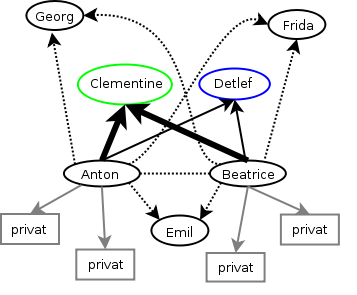
\includegraphics[scale=0.55]{../screenshots/kanalyse2.png}
\caption{Soziales Netz von Anton und Beatrice}
\label{abb:kanalyse1}
\end{center}
\end{figure}

Besonders h�ufig haben beide (zeitlich korreliert) Kontakt zu \textit{Clementine} und \textit{Detlef}. Diese beiden Personen scheinen eine wesentliche Rolle innerhalb der Gruppe ''mg`` zu spielen. Einige Personen k�nnen als offensichtlich privat aus der weiteren Analyse entfernt werden, da nur einer von beiden Kontakt h�lt und keine zeitlichen Korrelationen erkennbar sind.\\

Ideal w�re es, an dieser Stelle die Kommunikation von \textit{Clementine} und \textit{Detlef} n�her zu untersuchen. Beide sind aber vorsichtig und es besteht kein umfassender Zugriff auf die Kommunikationsdaten. Dann nimmt man als Ersatz vielleicht \textit{Frida}, um das Modell zu pr�zisieren.\\

Frida unterh�lt vor allem einen engen Kontakt zu \textit{Detlef}, was zu einer Umbewertung der Positionen von \textit{Detlef} und \textit{Clementine} f�hrt (Bild \ref{abb:kanalyse2}). Bei \textit{Emil} handelt es sich evtl. um einen zuf�llig gemeinsamen Bekannten von \textit{Anton} und \textit{Beatrice}, der nicht in die ''mg`` eingebunden ist.\\ 

\begin{figure}[htb]
\begin{center}
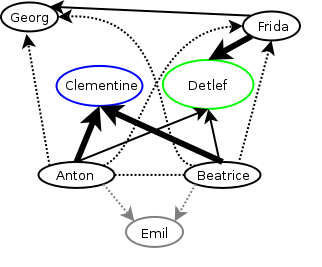
\includegraphics[scale=0.55]{../screenshots/kanalyse3.png}
\caption{Pr�zisierte Struktur der ''mg``}
\label{abb:kanalyse2}
\end{center}
\end{figure}

Reale Kommunikationsnetzwerke sind wesentlich komplexer. Auf Grundlage der Daten, die von T-Mobile �ber den Politiker Malte Spitz gespeichert wurden, hat Michael Kreil von OpenDataCity die Grafik in Bild \ref{abb:kanalyse3} erstellt.

\begin{figure}[htb]
\begin{center}
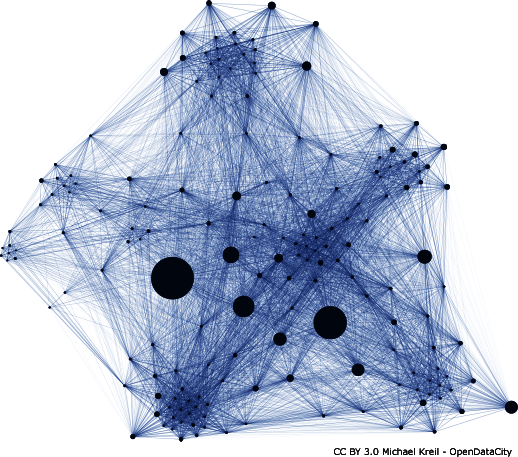
\includegraphics[scale=0.55]{../grafiken/cluster1_small.png}
\caption{Kommunikationsnetzwerk von Malte Spitz}
\label{abb:kanalyse3}
\end{center}
\end{figure}

\section{�berwachungen im Internet}
Unter \href{http://www.daten-speicherung.de/index.php/ueberwachungsgesetze/}{http://www.daten-speicherung.de/index.php/ueberwachungsgesetze} findet man eine umfassende �bersicht zu verschiedene Sicherheits-Gesetzen der letzten Jahre. Neben einer Auflistung der Gesetze wird auch dargestellt, welche Parteien des Bundestages daf�r und welche Parteien dagegen gestimmt haben. Sehr sch�n erkennbar ist das Muster der Zustimmung durch die jeweiligen Regierungsparteien und meist Ablehnung durch die Opposition, von B�swilligen als Demokratie-Simulation bezeichnet. Unabh�ngig vom Wahlergebnis wird durch die jeweiligen Regierungsparteien die �berwachung ausgebaut, denn \textbf{Du bist Terrorist!} \footnote{ \href{http://www.dubistterrorist.de/}{http://www.dubistterrorist.de}}
\begin{description}
\item[Vorratsdatenspeicherung oder Mindestspeicherfrist:] Ohne jeglichen Verdacht sollen die Verbindungsdaten jeder E-Mail, jedes Teleonats, jeder SMS und Standortdaten der Handys gesammelt werden.\\

Die Versuche zur Einf�hrung sind nicht neu. 1997 wurde die VDS aufgrund verfassungs�rechtlicher Bedenken abgelehnt, 2002 wurde ein �hnlicher Gesetzentwurf vom Deutschen Bundestag abgelehnt und die Bundesregierung beaufragt, gegen einen entsprechenden Rahmenbeschlu� auf EU-Ebene zu stimmen (siehe Bundestag-Drucksache 14/9801). Der Wissenschaftliche Dienst des Bundestages hat bereits 2006 ein Rechtsgutachten mit schweren Bedenken gegen die VDS vorgelegt.\\

Ein Vergleich der Zahlen der Kriminalit�tsstatistik des BKA f�r die Jahre 2007, 2008 und 2009 zeigt, dass die VDS im Jahr 2009 nicht zur einer Verbesserung der Aufkl�rungsrate von Straftaten im Internet f�hrte und keine Einfluss auf die Tendenz der Entwicklung hatte. Es gibt mehr Straftaten im Internet bei abnehmender Aufkl�rungsrate.

\begin{center}
\begin{tabular}{l|c|c|c|c}
 & 2007 & 2008 & 2009 & 2010\\
& (o. VDS) & (o. VDS) & (\textbf{mit VDS}) &  (o. VDS)\\
\hline
Straftaten im Internet & 179.026 & 167.451 & 206.909 & 223.642\\
Aufkl�rungsrate (Internet) & 82.9\% & 79.8\% & 75.7\% & 72,3\%\\
\end{tabular}
\end{center}

Eine umfangreiche wissenschaftliche Analyse des Max-Planck-Instituts (MPI) f�r ausl�ndisches und internationales Strafrecht belegt, dass KEINE \textit{Schutzl�cke} ohne Vorratsdatenspeicherung besteht und widerspricht damit der Darstellung von mehreren Bundesinnenministern und BKA-Chef Ziercke, wonach die VDS f�r die Kriminalit�ts�bek�mpfung unbedingt n�tig w�re. Die in der Presse immer wieder herangezogenen Einzelbeispiele halten einer wissenschaftlichen Analyse nicht stand.\\ 

In einem offenen Brief sprachen sich Richter und Staatsanw�lte gegen die VDS aus und widersprechen ebenfalls der Notwendigkeit f�r die Kriminalit�tsbek�mpfung.

\item[Zensur im Internet:] Die Zensur sollte in Deutschland im Namen des Kampfes gegen Kinderpornografie im Internet eingef�hrt werden. Man wurde nicht m�de zu behaupten, es g�be einen Millionen Euro schweren Massenmarkt, der durch Sperren von Websites empfindlich ausgetrocknet werden kann. Die Aussagen wurden �berpr�ft und f�r falsch befunden \footnote{ \href{http://blog.odem.org/2009/05/quellenanalyse.html}{http://blog.odem.org/2009/05/quellenanalyse.html}}.
\begin{enumerate}
\item In der ersten Stufe unterzeichneten im Fr�hjahr 2009 die f�nf gro�en Provider freiwillig einen geheimen Vertrag mit dem BKA. Sie verpflichteten sich, eine Liste von Websites zu sperren, die vom BKA ohne nennenswerte Kontrolle erstellt werden sollte.
\item In der zweiten Stufe wurde am 18.06.09 das \textit{Zugangserschwernisgesetz} verabschiedet. Alle Provider mit mehr als 10.000 Kunden sollen diese geheime Liste von Websites zu sperren. Neben den (ungeeigneten) DNS-Sperren sollen auch IP-Sperren und Filterung der Inhalte zum Einsatz kommen.
\item Die CDU/FDP-Regierung ist im Herbst 2009 einen halben Schritt zur�ck gegangen und hat mit einem Anwendungserlass die Umsetzung des Gesetzes f�r ein Jahr aufgeschoben. Diese Regierung meint also, �ber dem Parlament zu stehen und ein beschlossenes Gesetz nicht umsetzen zu m�ssen.
\item Im Rahmen der Evaluierung des Gesetzes geht das BKA nur halbherzig gegen dokumentierten Missbrauch vor, wie eine Ver�ffentlichung des AK-Zensur zeigt. Gleichzeitig wird weiter Lobbyarbeit f�r das Zensurgesetz betrieben \footnote{ \href{http://ak-zensur.de/2010/08/kapitulation.html}{http://ak-zensur.de/2010/08/kapitulation.html}}.
\item Die Auswertung des eco Verband zeigt, dass Webseiten mit dokumentiertem Missbrauch effektiv gel�scht werden k�nnen. 2010 wurden 99,4\% der gemeldeten Webseiten gel�scht \footnote{ \href{http://www.eco.de/verband/202\_8727.htm}{http://www.eco.de/verband/202\_8727.htm}}.
\item Im Herbst 2011 wurde das Gesetz offiziell beerdigt.
\end{enumerate}

Der Aufbau einer Infrastruktur f�r Zensur im Internet wird auf vielen Wegen betrieben. Neben dem Popanz \textit{``Kinderpornografie``} engagiert sich die Content Maffia im Rahmen der geheimen ACTA Verhandlungen f�r eine verbindliche Verpflichtung zum Aufbau der Infrastruktur f�r Websperren. Die CDU/CSU Bundestagsfraktion sieht die amerikanischen Gesetzesvorlagen SOPA und PIPA als richtungsweisend an. Beide Gesetzesvorlagen sehen umfangreiche Zensurma�nahmen zum Schutz geistigen Eigentums vor.\\

Die verfassungsrechlichen Bedenken gegen die Zensur hat der wissenschaftliche Dienst des Bundestages in einem Gutachten zusammengefasst\footnote{ \href{http://netzpolitik.org/wp-upload/bundestag\_filter-gutachten.pdf}{http://netzpolitik.org/wp-upload/bundestag\_filter-gutachten.pdf}}. Auch eine Absch�tzung der EU-Kommision kommt zu dem Schluss, dass diese Sperrma�nahmen \textbf{notwendigerweise eine Einschr�nkung der Menschenrechte voraussetzen}, beispielsweise der freien Meinungs�u�erung. 

\item[BKA Gesetz:] Mit dem BKA Gesetz wurde eine Polizei mit den Kompetenzen eines Geheimdienstes geschaffen. Zu diesen Kompetenzen geh�ren neben der heimlichen Online-Durchsuchung von Computern der Lauschangriff au�erhalb und innerhalb der Wohnung (incl. Video), Raster- und Schleierfahndung, weitgehende Abh�rbefugnisse, Einsatz von V-Leuten, verdeckten Ermittlern und informellen Mitarbeitern...\\

Im Rahmen pr�ventiver Ermittlungen (d.h. ohne konkreten Tatverdacht) soll das BKA die Berechtigung erhalten, in eigener Regie zu handeln und Abh�rma�nahmen auch auf Geistliche, Abgeordnete, Journalisten und Strafverteidiger auszudehnen. Im Rahmen dieser Vorfeldermittlungen unterliegt das BKA nicht der Leitungsbefugnis der Staatsanwaltschaft.\\

\textit{Damit wird sich das BKA bis zu einem gewissen Grad jeglicher Kontrolle, der justiziellen und erst recht der parlamentarischen, entziehen k�nnen \footnote{ \href{http://www.berlinonline.de/berliner-zeitung/print/politik/725127.html}{http://www.berlinonline.de/berliner-zeitung/print/politik/725127.html}}.}
\item[Telekommunikations�berwachungsverordnung] Auf richterliche Anordnung wird eine Kopie der gesamten Kommunikation an Strafverfolgungsbeh�rden weitergeleitet. Dieser Eingriff in das verfassungsm��ig garantierte Recht auf unbeobachtete Kommunikation ist nicht nur bei Verdacht schwerer Verbrechen m�glich, sondern auch bei einigen mit Geldstrafe bew�hrten Vergehen und sogar bei Fahrl�ssigkeitsdelikten (siehe �100a StPO).\\

Laut Gesetz kann die �berwachung auch ohne richterliche Genehmigung begonnen werden. Sie ist jedoch sp�testens nach 3 Tagen einzustellen, wenn bis dahin keine richterliche Genehmigung vorliegt.

\item[Pr�ventiv-polizeil. Telekommunikations�berwachung] erm�glicht es den Strafverfolgungsbeh�rden der L�nder Bayern, Th�ringen, Niedersachsen, Hessen und Rheinland-Pfalz den Telefon- und E-Mail-Verkehr von Menschen mitzuschneiden, die keiner(!) Straftat verd�chtigt werden. Es reicht aus, in der N�he eines Verd�chtigten zu wohnen oder m�glicherweise in Kontakt mit ihm zu stehen.\\

Die Anzahl der von dieser Ma�nahme Betroffenen verdoppelt sich Jahr f�r Jahr. Gleichzeitig f�hren nur 17\% der �berwachungen zu Ergebnissen im Rahmen der Ermittlungen.

\item[Zugriff auf \textit{Bestandsdaten} bei Providern] Der IT-Sicherheitsforscher Pete Swire hat im April 2012 ein Paper \footnote{ \href{https://papers.ssrn.com/sol3/papers.cfm?abstract\_id=2038871}{https://papers.ssrn.com/sol3/papers.cfm?abstract\_id=2038871}} ver�ffentlicht, in dem er die aktuellen Tendenzen in der �berwachung aufzeigt. Geheimdienste und Strafverfolger dr�ngen auf Zugriff auf die \textit{Daten in der Cloud}. Dazu z�hlen auch E-Mail Accounts. Die H�rden f�r den Zugriff sollen dabei m�glichst gering sein.\\

Mit der Reform der Telekommuniukations�berwachung im Dezember 2012 kommt der Gesetzgeber den W�nschen der Geheimdienste weit entgegen. Ohne richterliche Pr�fung d�rfen die \textit{Dienste} die sogenannten Bestandsdaten abfragen. Die Cloud-Provider und Mail-Provider sollen automatisiert nutzbare Schnittstellen daf�r bereitstellen. Zu den Bestandsdaten z�hlen seit Dezember 2012 neben Name und Anschrift auch:
\begin{itemize}
 \item Passworte f�r den Zugriff auf E-Mail Konten und Cloud-Speicher.
 \item PINs zum Entsperren von Smartphones.
 \item Zugriff auf die Endger�te (Router), die den Kunden vom DLS-Provider kostenlos bereitgestellt werden (TR-069 Schnittstelle).
\end{itemize}
Die PiratenPartei kommentierte den Gesetzentwurf kurz und b�ndig:
\begin{quote}
 \textit{Der Entwurf der Bundesregierung ist schlicht verfassungswidrig.}
\end{quote} 


\item[Datenbanken:] Begleitet werden diese Polizei-Gesetze vom Aufbau umfangreicher staatlicher Datensammlungen. Von der Schwarze Liste der Ausl�nderfreunde (Einlader-Datei) bis zur AntiTerrorDatei, die bereits 20.000 Personen enth�lt, obwohl es in Deutschland keinen Terroranschlag gibt. (Abgesehen von den Muppets aus dem Sauerland, deren Islamische Jihad Union offensichtlich eine Erfindung der Geheimdienste ist.)

\item[Elektronisicher PA:] Mit dem Elektronischen Personalausweis wird die biometrische Voll-Erfassung der Bev�lkerung voran getrieben. Au�erdem werden die Grundlagen f�r eine eindeutige Identifizierung im Internet gelegt, begleitet von fragw�rdigen Projekten wie De-Mail.
\end{description} 

\subsubsection*{Der Elektronische Polizeistaat}
\begin{quote}
   \textit{W�rde man noch den Mut haben, gegen die Regierung zu opponieren, wenn diese Einblick in jede Email, in jede besuchte Porno-Website, jeden Telefonanruf und jede �berweisung hat?}
\end{quote} 

Was unterscheidet einen elektronischen Polizeistaat von einer Diktatur? Gibt es dort auch eine Geheime Bundespolizei, die Leute nachts aus der Wohnung holt und abtransportiert, ohne juristischen Verfahren einsperrt...\\

Ein elektronischer Polizeistaat arbeitet sauberer. Es werden elektronische Technologien genutzt um forensische Beweise gegen B�rgerInnen aufzuzeichnen, zu organisieren, zu suchen und zu verteilen. Die Informationen \underline{werden unbemerkt und umfassend gesammelt}, um sie bei Bedarf f�r ein juristisches Verfahren als Beweise aufzubereiten.\\

Bei einem Vergleich von 52 Staaten hinsichtlich des Ausbaus des elektronischen Polizeistaat hat Deutschland einen beachtlichen 10 Platz belegt. Es verwundert nicht, dass an erster Stelle China und Nordkorea, gefolgt von Wei�russland und Russland stehen. Dann aber wird bereits Gro�britannien aufgelistet, gefolgt von den USA, Singapur, Israel, Frankreich und Deutschland.

\begin{quote}
   \textit{Noch sei der Polizeistaat nicht umfassen realisiert, ``aber alle Fundamente sind gelegt''. Es sei schon zu sp�t, dies zu verhindern. Mit dem Bericht wolle man die Menschen darauf aufmerksam machen, dass ihre Freiheit bedroht ist.}
\end{quote} 

\begin{figure}[htb]
\begin{center}
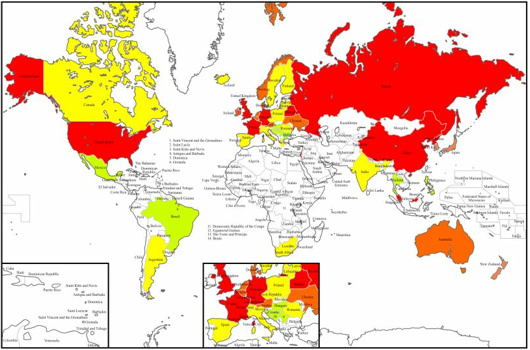
\includegraphics[scale=0.5]{../grafiken/polizeistaat.jpg}
\caption{Vergleich der elektronischen Polizeistaaten}
\label{abb:polizeistaat}
\end{center}
\end{figure}

Das dieser Polizeistaat bereits arbeitsf�hig ist, zeigt die Aff�re J�rg Tauss. Ein unbequemer Politiker mit viel zu engen Kontakten zum CCC, der Datenschutz ernst nimmt, gegen das BKA-Gesetz und gegen Zensur auftritt, wird wenige Monate vor der Wahl des Konsums von KiPo verd�chtigt. Die Medien st�rzen sich auf das Thema. Innerhalb kurzer Zeit war Tauss als Politiker von der Springer-Presse demontiert, unabh�ngig von der sp�ter folgenden Verurteilung. \\

�hnliche Meldungen hatten in den letzten Jahren viel weniger Resonanz:
\begin{enumerate}
 \item \textit{Auf dem Dienstcomputer eines hochrangigen Mitglieds des hessischen Innenministeriums sind vermutlich Kinderpornos entdeckt worden.} (25.07.2007)
\item \textit{Kinderpornos: CDU-Politiker unter Verdacht} (01.04.2005)
\item \textit{Der CDU-Politiker Andreas Zwickl aus Neckarsulm ist wegen Verdachts des Besitzes von Kinderpronografie...} (05.03.2009)
\end{enumerate}

\section{Rechtsstaatliche Grundlagen}
\begin{quote}
\textit{Es ist erkennbar, wohin die Reise gehen soll. Die R�der rollen bereits.\\
Es wird Zeit, ein neues Ziel zu buchen, bevor der Zug  abgefahren ist.}
\end{quote} 

Die Kriminaliserung der Protestler gegen den G8-Gipfel in Heiligendamm als Terroristen, die Diskussion um die weitr�umige Funkzellenauswertung anl��lich der Anti-Nazi-Demo in Dresden 2011 und das Gutachten des Bundesdatenschutzbeauftragten zum \textit{Staatstrojaner} zeigen deutlich die gesellschaftlichen Defizite bei der Begrenzung der �berwachung.\\

Der teilweise erfolgreiche Widerstand der Zivilgesellschaft gegen Vorratsdatenspeicherung, Zugangserschwernisgesetz, Online Durchsuchung, Gro�er Lauschangriff usw. reicht nicht aus. Die gesellschaftlich ausgehandelten Normen (Gesetze, Urteile des BVerfG...) zur Begrenzung der �berwachung werden nicht respektiert und scheinbar systematisch und ohne Konsequenzen f�r die Verantwortlichen missachtet.

\subsubsection*{Gedanken f�r eine Gegenstrategie}
\begin{enumerate}
 \item Die Einhaltung der Normen f�r Polizei und Geheimdienste, die in einer demokratischen Diskussion ausgehandelt und als Gesetze bzw. Urteile des BVerfG niedergeschrieben sind, muss besser kontrolliert werden. Eine optionale Kontrolle ist unbrauchbar.\\

 Auf der Veranstaltung \textit{Soziale Bewegungen im Digitalen Tsunami} hat Dr. Thilo Weichert (ULD) die Situation aus Sicht des Datenschutz treffend beschrieben:
\begin{quote}
\textit{Die Polizeibeh�rden fragen uns nur, wenn sie wissen, das wir unser Ok geben.}
\end{quote}

\item Verst��e der Strafverfolger gegen geltendes Recht m�ssen geahndet werden, so wie es bei Verst��en gegen Gesetze auf anderen Gebieten �blich ist. Bisher agieren Straf�verfolger scheinbar in einem ``rechtsfreien Raum``. �bertretungen der zul�ssigen Grenzen haben keine oder (bei starkem �ffentlichen Druck) harmlose Konsequenzen.

\item Die Besetzung der Posten von Entscheidungstr�gern bei Polizei und Geheimdiensten sollte mit Personen erfolgen, die sich dem ausgehandelten Konsens verpflichtet f�hlen. Wenn der neue Polizeipr�sident von Dresden die weitr�umige Funk�zellen��berwachung in Dresden f�r richtig h�lt und in einer �hnlichen Situation wieder zu diesem Mittel greifen will, obwohl es f�r rechtswidrig erkl�rt wurde, dann ist er f�r die Aufgabe ungeeignet.\\

Udo Vetter stellt im lawblog die Frage:
\begin{quote}
\textit{Wurde hier bewusst auf dem Rechtsstaat rumgetrampelt - oder sind die Verantwortlichen einfach so doof?}
\end{quote}

\item Auf Basis des �129a StGB (Bildung einer terroristisichen Vereinigung) wurden in den letzten Jahren so gut wie keine Verurteilungen ausgesprochen. Die sehr weit gehenden Befugnisse f�r Ermittlungen nach diesem Paragraphen wurden jedoch mehrfach genutzt, um politische Aktivisten auszuforschen. Mehrfach haben verschiedene Gerichte die Anwendung des �129a StGB durch Ermittlungsbeh�rden f�r illegal erkl�rt.
\begin{itemize}
 \item Doppeleinstellung in Sachen �129 \footnote{ \href{http://de.indymedia.org/2008/10/228421.shtml}{http://de.indymedia.org/2008/10/228421.shtml}}
 \item Razzien im Vorfeld des G8-Gipfels waren rechtswidrig \footnote{ \href{http://www.ag-friedensforschung.de/themen/Globalisierung/g8-2007/bgh.html}{http://www.ag-friedensforschung.de/themen/Globalisierung/g8-2007/bgh.html}}
 \item Konstruieren und schn�ffeln mit �129a \footnote{ \href{http://www.neues-deutschland.de/artikel/175230.konstruieren-und-schnueffeln-mit-s-129a.html}{http://www.neues-deutschland.de/artikel/175230.konstruieren-und-schnueffeln-mit-s-129a.html}}
 \item Durchsuchung beim LabourNet waren rechtswidrig \footnote{ \href{http://www.labournet.de/ueberuns/beschlagnahme/index.html}{http://www.labournet.de/ueberuns/beschlagnahme/index.html}}
\end{itemize}
Dieser Missbrauch der Anti-Terror Befugnisse sollte gestoppt und evaluiert werden.
\end{enumerate}

\section{Bundesamt f�r Verfassungsschutz aufl�sen}
Es wird Zeit, das Bundesamt f�r Verfassungsschutz aufzul�sen. Die Humanistische Union fordert bereits seit 20 Jahren die Aufl�sung dieses Inlandgeheimdienstes. Seine Aufgabe als Bollwerk gegen die drohende Infiltration feindlicher Agenten aus der Sowjetunion oder der DDR besteht nicht mehr. Anti-Spionage und Anti-Terror Eins�tze sowie Bek�mpfung der Korruption und Verfolgung von Sachbesch�digungen sind Aufgabe der Polizei.\\

\subsubsection*{V-Leute sind keine L�sung, sondern das Problem}
\begin{quote}
\textit{Geheimdienste ... sind nach wie vor die gro�e Unbekannte in der Entstehung und Entwicklung des Terrorismus, des bundesdeutschen ebenso wie des mit ihm verflochtenen internationalen Terrorismus.} (W. Kraushaar)
\end{quote}

\begin{itemize}
 \item V-Leute des Verfassungsschutz hatten erheblichen Anteil an der Radikalisierung der Studentenbewegung 1968. Vor allem der V-Mann Peter Urbach wird immer wieder als Agent Provocateur genannt, der auch Waffen und Molotow-Cocktails lieferte und nach seiner Entarnung vom Verfassungsschutz ins Ausland gebracht wurde.\footnote{ \href{http://www.heise.de/tp/blogs/8/151641}{http://www.heise.de/tp/blogs/8/151641}}

 \item Die Verflechtungen von Verfassungsschutz und \textit{RAF} sind noch immer nicht aufgekl�rt. Aus alten Unterlagen der Stasi geht hervor, dass Verena Becker vom Verfassungs�schutz ''kontrolliert wurde''. V. Becker spielte eine wesentliche Rolle beim 
Mord an Generalbundesanwalt Buback.\footnote{ \href{http://www.heise.de/tp/artikel/31/31120/1.html}{http://www.heise.de/tp/artikel/31/31120/1.html}}

 \item Der Verfassungsschutz hat die rechtsradikale Szene nicht unterwandert, sondern finanziell unterst�tzt und vor Strafverfolgung gesch�tzt.
\begin{itemize}
 \item Laut einem BKA-Report \footnote{ \href{http://www.spiegel.de/panorama/justiz/verfassungsschutz-soll-rechte-v-leute-vor-strafverfolgung-geschuetzt-haben-a-865154.html}{http://www.spiegel.de/panorama/justiz/verfassungsschutz-soll-rechte-v-leute-vor-strafverfolgung-geschuetzt-haben-a-865154.html}} von 1997 soll der Verfassungsschutz rechtsradikale Neonazis systematisch gesch�tzt haben. Die Vorw�rfe werden mit konkreten F�llen untermauert. 
V-Leute wurden vor Durchsuchungen gewarnt und einer Straftat �ber�f�hrte Nazis wurden nicht angeklagt und verurteilt, wenn sie als V-Leute arbeiteten. Informationen wurde zu sp�t an die Polizei weitergeleitet, so dass rechtsradikale Aktionen nicht mehr verhindert werden konnten.
 \item Bereits 2002 hat das LKA Sachsen-Anhalt dem Verfassungsschutz misstraut und aus \textit{ermittlungstaktischen Gr�nden} nicht �ber Exekutivma�nahmen in der rechten Szene informiert. Aus einem Vermerk des Bundesinnenministeriums:\footnote{ \href{https://www.taz.de/Neonazi-Ermittlungen/!103340/}{https://www.taz.de/Neonazi-Ermittlungen/!103340/}}
  \begin{quote}
   \textit{Nach R�cksprache (...) st�tzen sich die ``ermittlungstaktischen Gr�nde`` vermutlich auf die Bef�rchtung, die Verfassungsschutzbeh�rden w�rden ihre Quellen �ber bevorstehende Exekutivma�nahmen informieren.}
  \end{quote} 
 \item 2008 wurden Ermittlungen gegen den Neonazi Sebastian Seemann eingestellt. Er baute das verbotene\textit{ Blood and Honour} Netzwerk auf und war im schwer�kriminellen Millieu aktiv (Drogen- und Waffenhandel). Der Verfassungsschutz warnte ihn vor Exekutivma�nahmen. Auf Veranlassung des Innenministers Dr. Ingo Wolff wurden auch Anklagen gegen die Mitarbeiter des Verfassungsschutz wegen Geheimnisverrats und Strafvereitelung eingestellt.\footnote{ \href{http://www.nadir.org/nadir/initiativ/azzoncao/donazi3.html}{http://www.nadir.org/nadir/initiativ/azzoncao/donazi3.html}}
\end{itemize}
Das ist seit mehreren Jahren bekannt. Konsequenzen? Keine!

 \item Die mit viel Brimborium verurteilte \textit{Sauerl�nder Terrorzelle} wurde vom V-Mann Mevl�t Kar gegr�ndet und f�r die Vorbereitung \textit{gigantischer Terroranschl�ge} mit Sprengz�ndern usw. versorgt. Die Sauerlandgruppe war der dritte Versuch von Mevl�t Kar, eine Terrorzelle aufzubauen und an die Beh�rden zu verraten.  M. Kar wurde nie angeklagt.\footnote{ \href{http://www.heise.de/tp/artikel/35/35986/1.html}{http://www.heise.de/tp/artikel/35/35986/1.html}}
\begin{itemize}
 \item Die erste Terrorzelle mit Mutlu A., Mohamed El-A. und Issam El-S wurde am 17. Februar 2003 von der GSG9 verhaftet und am gleichen Tag aus Mangel an Beweisen wieder freigelassen.
\item Die Verhaftung der zweiten Terrorzelle mit Dzavid B., Nedzad B., Ahmed H., Bekim T. und Blerim T. wurde von den Medien weitgehend ignoriert.
\end{itemize}

 \item Ein weiterer V-Mann des Verfassungsschutz in der islamistischen Szene war Yehia Yousif, der mittlerweile in Saudi-Arabien lebt und auch eine Schl�sselrolle in der Radikalisierung der Sauerland Gruppe spielte. Yousif hat wesentlich zum Erstarken salafitischer Gruppen beigetragen.\footnote{ \href{http://www.heise.de/tp/blogs/8/150854}{http://www.heise.de/tp/blogs/8/150854}}

 \item Die \textit{Globale Islamische Medienfront} (GIMF) drohte 2007 in Videos mit Terroranschl�gen in Deutschland. Im Gerichtsverfahren gegen Mitglieder der GIMF kam heraus, dass der Anf�hrer dieser Gruppe ein V-Mann des Verfassungsschutzes war. Irfan P. soll monatlich 2.500 - 3.000 Euro vom Verfassungs�schutz erhalten haben. Gegen den V-Mann wurde ebenfalls keine Anklage erhoben.\footnote{ \href{http://www.heise.de/tp/blogs/8/150854}{http://www.heise.de/tp/blogs/8/150854}}

 \item Die Rolle des Verfassungsschutz bei den systematischen Pannen im Rahmen der Ermittlungen zur \textit{rechtsradikalen NSU Terrorzelle} wird sicher nicht vollst�ndig aufgekl�rt werden.
\end{itemize}
Ohne die zweifelhafte Rolle der V-Leute w�rden wir ruhiger leben und viele Sicherheitsgesetze w�ren nicht durchsetzbar gewesen.

\subsubsection*{�berwachung politischer Aktivisten}
Der Verfassungsschutz entwickelt sich zu einem Geheimdienst zur �berwachung von politischen Aktivisten und unliebsamen Abgeordneten. 
\begin{itemize}
 \item R. G�ssler: 38 Jahre zu Unrecht vom Verfassungschutz �berwacht \footnote{ \href{http://heise.de/-217246}{http://heise.de/-217246}}

 \item Verfassungsschutz in Bayern �berwacht die linke Szene \footnote{ \href{http://www.heise.de/tp/artikel/35/35942/1.html}{http://www.heise.de/tp/artikel/35/35942/1.html}}

 \item �berwachung einer linken Gruppe durch Verfassungsschutz \footnote{ \href{http://www.heise.de/tp/blogs/8/151499}{http://www.heise.de/tp/blogs/8/151499}}

 \item Verfassungsschutz bespitzelt linke Abgeordnete \footnote{ \href{http://www.heise.de/tp/artikel/36/36316/1.html}{http://www.heise.de/tp/artikel/36/36316/1.html}}

 \item Gegner von Stuttgart21 vom Verfassungsschutz �berwacht \footnote{ \href{http://www.bei-abriss-aufstand.de/2012/02/25/bespitzelt-der-verfassungsschutz-parkgebete/}{http://www.bei-abriss-aufstand.de/2012/02/25/}}

 \item mg-�berwachung durch den Verfassungsschutz war illegal \footnote{ \href{http://annalist.noblogs.org/post/2012/03/03/mg-uberwachung-durch-den-verfassungsschutz-war-illegal/}{http://annalist.noblogs.org/post/2012/03/03/}}

 \item Ohne demokratische Kontrolle (BfV in Bayern) \footnote{ \href{http://www.heise.de/tp/artikel/35/35942/1.html}{http://www.heise.de/tp/artikel/35/35942/1.html}}
\end{itemize}

\section{Ich habe doch nichts zu verbergen}
Dies Argument h�rt man oft. Haben wir wirklich nichts zu verbergen? Einige Beispiele sollen exemplarisch zeigen, wie willk�rlich gesammelte Daten unser Leben gravierend beeinflussen k�nnen:

\begin{itemize}
 \item Im Rahmen der Zul�ssigkeitspr�fung f�r Piloten wurde Herr J. Schreiber mit den vom Verfassungsschutz gesammelten Fakten konfrontiert \footnote{ \href{http://www.pilotundflugzeug.de/artikel/2006-02-10/Spitzelstaat}{http://www.pilotundflugzeug.de/artikel/2006-02-10/Spitzelstaat}}:

\begin{enumerate}
 \item Er wurde 1994 auf einer Demonstration kontrolliert. Er wurde nicht angezeigt, angeklagt oder einer Straftat verd�chtigt, sondern nur als Teilnehmer registriert.
\item Offensichtlich wurde daraufhin sein Bekanntenkreis durchleuchtet.
\item Als Gesch�ftsf�hrer einer GmbH f�r Softwareentwicklung habe er eine vorbestrafte Person besch�ftig. Er sollte erkl�ren, welche Beziehung er zu dieser Person habe.
\item Laut Einsch�tzung des Verfassungsschutzes neige er zu politischem Extremismus, da er einen Bauwagen besitzt. Bei dem sogenannten \textit{Bauwagen} handelt es sich um einen Allrad-LKW, den Herr S. f�r Reisen nutzt (z.B. in die Sahara).
\end{enumerate}
F�r Herrn S. ging die Sache gut aus. In einer Stellungnahme konnte er die in der Akte gesammelten Punkte erkl�ren. In der Regel wird uns die Gelegenheit einer Stellungnahme jedoch nicht einger�umt.

\item Ein junger Mann meldet sich freiwillig zur Bundeswehr. Mit sechs Jahren war er kurzzeitig in therapheutischer Behandlung, mit vierzehn hatte er etwas gekifft. Seine besorgte Mutter ging mit ihm zur Drogenberatung. In den folgenden Jahren gab es keine Drogenprobleme. Von der Bundeswehr erh�lt er eine Ablehnung, da er ja mit sechs Jahren eine Psychotherapie durchf�hren musste und Drogenprobleme gehabt h�tte. \footnote{ 
\href{http://blog.kairaven.de/archives/998-Datenstigmaanekdote.html}{http://blog.kairaven.de/archives/998-Datenstigmaanekdote.html}}.

\item Kollateralsch�den: Ein gro�er deutscher Provider liefert falsche Kommunikationsdaten ans BKA. Der zu Unrecht Beschuldigte erlebt das volle Programm: Hausdurchsuchung, Beschlagnahme der Rechner, Verh�re und sicher nicht sehr lustige Gespr�che im Familienkreis. Die pers�nlichen und wirtschaftlichen Folgen sind schwer zu beziffern \footnote{ 
\href{http://www.lawblog.de/index.php/archives/2008/03/11/provider-liefert-falsche-daten-ans-bka/}{http://www.lawblog.de/index.php/archives/2008/03/11/}}.\\

Noch krasser ist das Ergebnis der \textit{Operation Ore} in Gro�britannien. 39 Menschen, zu Unrecht wegen Konsums von Kinderpornografie verurteilt, haben Selbstmord begangen, da ihnen alles genommen wurde \footnote{ \href{http://en.wikipedia.org/wiki/Operation\_Ore}{http://en.wikipedia.org/wiki/Operation\_Ore}}.

\item ``Leimspur des BKA'': Wie schnell man in das Visier der Fahnder des BKA geraten kann, zeigt ein Artikel bei Zeit-Online. Die Webseite des BKA zur Gruppe ``mg'' ist ein Honeypot, der dazu dient, weitere Sympathisanten zu identifizieren. Die Bundesanwaltschaft verteidigt die Ma�nahme als legale Fahndungsmethode.\\

Mit dem im Juni 2009 beschlossenen BSI-Gesetz �bernimmt die Beh�rde die Aufzeichnung und unbegrenzte Speicherung personenbezogener Nutzerinformationen wie IP-Adressen, die bei der Online-Kommunikation zwischen B�rgern und Verwaltungseinrichtungen des Bundes anfallen. Ich kann daraus nur den Schluss ziehen, diese und �hnliche Angebote in Zukunft ausschlie�lich mit Anonymisierungsdiensten zu nutzen.
\end{itemize}

Nicht immer treten die (repressiven) Folgen staatlicher Sammelwut f�r die Betroffenen so deutlich hervor. In der Regel werden Entscheidungen �ber uns getroffen, ohne uns zu benachrichtigen. Wir bezeichnen die (repressiven) Folgen dann als Schicksal.

\subsection*{Politische Aktivisten}
Wer sich politisch engagiert und auf gerne vertuschte Mi�st�nde hinweist, hat besonders unter der Sammelwut staatlicher Stellen zu leiden. Wir m�chte jetzt nicht an Staaten wie Iran oder China m�keln. Einige deutsche Beispiele:

\begin{enumerate}
\item Erich Schmidt-Eenboom ver�ffentliche 1994 als Publizist und Friedensforscher ein Buch �ber den BND. In den folgenden Monaten wurden er und seine Mitarbeiter vom BND ohne rechtliche Grundlage intensiv �berwacht, um die Kontaktpersonen zu ermitteln. Ein Interview unter dem Titel \textit{``Sie beschatteten mich sogar in der Sauna''} \footnote{ \href{http://www.spiegel.de/politik/deutschland/0,1518,384374,00.html}{http://www.spiegel.de/politik/deutschland/0,1518,384374,00.html}} gibt es bei SPON.
\item Fahndung zur Abschreckung: In Vorbereitung des G8-Gipfels in Heiligendamm veranstaltete die Polizei am 9. Mai 2007 eine Gro�razzia. Dabei wurden bei Globalisierungsgegnern Rechner, Server und Materialien beschlagnahmt. Die Infrastruktur zur Organisation der Proteste wurde nachhaltig gesch�digt. Wenige Tage nach der Aktion wurde ein Peilsender des BKA am Auto eines Protestlers gefunden. Um die pr�ventiven Ma�nahmen zu rechtfertigen, wurden die Protestler als terroristische Vereinigung eingestuft. 
Das Netzwerk ATTAC konnte 1,5 Jahre sp�ter vor Gericht erreichen, dass diese Einstufung unrechtm��ig war. Das Ziel, die Organisation der Proteste zu behindern, wurde jedoch erreicht.
\item Dr. Rolf G�ssner ist Rechtsanwalt, Vizepr�sident der Internationalen Liga f�r Menschenrechte, Mitherausgeber des Grundrechte-Reports, Vizepr�sident  und Jury-Mitglied bei den Big Brother Awards. Er wurde vom Verfassungsschutz 38 Jahre lang �berwacht. Obwohl das Verwaltungsgericht K�ln bereits urteilte, dass der Verfassungsschutz f�r den gesamten Bespitzelungszeitraum Einblick in die Akten gew�hren muss, wird dieses Urteil mit Hilfe der Regierung ignoriert. Es werden Sicherheitsinteressen vorgeschoben!
\end{enumerate}

Mit dem Aufbau der ``neuen Sicherheitsarchitektur'' bedeutet eine �berwachung nicht nur, dass der direkt Betroffene �berwacht wird. Es werden Bekannte und Freunde aus dem pers�nlichen Umfeld einbezogen. Sie werden in der AntiTerrorDatei gespeichert, auch ihre Kommunikation kann �berwacht werden, es ist sogar m�glich, Wanzen in den Wohnungen der Freunde zu installieren.

\chapter{Digitales Aikido}
Die folgende grobe �bersicht soll die Orientierung im Dschungel der nachfolgend beschriebenen M�glichkeiten etwas erleichtern.

\begin{itemize}
 \item \textbf{Einsteiger:} Datensammler nutzen verschiedene M�glichkeiten, Informationen �ber die Nutzer zu generieren. Die Wiedererkennung des Surfers bei der Nutzung verschiedener Dienste kann mit einfachen Mitteln erschwert werden. (Datensammler meiden und Alternativen nutzen, Cookies und JavaScript kontrollieren, Werbung filtern, SSL-verschl�sselte Verbindungen nutzen, E-Mail Client sicher konfigurieren...)

\item \textbf{1. Grad:} Zensur umgehen. Immer mehr L�nder f�hren Zensur-Ma�nahmen ein, um den Zugriff auf unerw�nschte Inhalte zu sperren. Mit den \textit{Simple Tricks} oder unzensierten DNS-Servern k�nnen diese Sperren umgangen werden.

\item \textbf{2. Grad:} Pers�nliche Daten und Inhalte der Kommunikation werden verschl�sselt. Das verwehrt unbefugten Dritten, Kenntnis von pers�nliche Daten zu erlangen. (Festplatte und Backups verschl�sseln mit Truecrypt, DM-Crypt oder FileVault, E-Mails verschl�sseln mit GnuPG oder S/MIME, Instant Messaging mit OTR...)

\item \textbf{3. Grad:} Anhand der IP-Adresse ist ein Nutzer eindeutig identifizierbar. Im Rahmen der Vorratsdatenspeicherung werden diese Daten f�r 6 Monate gespeichert. Mixkaskaden (JonDonym) oder Onion Router (Tor) bieten eine dem realen Leben vergleichbare Anonymit�t. Remailer bieten die M�glichkeit, den Absender einer E-Mail zu verschleiern.

\item \textbf{4. Grad:} Eine noch h�here Anonymit�t bietet das \textit{Invisible Internet Projekt} (I2P) oder das \textit{Freenet Projekt}. Eine dezentrale und vollst�ndig verschl�sselte Infrastruktur verbirgt die Inhalte der Kommunikation und wer welchen Dienst nutzt. Auch Anbieter von Informationen sind in diesen Netzen anonym.
\end{itemize}
Die einzelnen Level bauen aufeinander auf! Es macht wenig Sinn, die IP-Adresse zu verschleiern, wenn man anhand von Cookies eindeutig identifizierbar ist. Auch die Versendung einer anonymen E-Mail ist in der Regel verschl�sselt sinnvoller.

\section{Nachdenken}
Eine Graduierung in den Kampfsportarten ist keine Garantie, dass man sich im realen Leben erfolgreich gegen einen Angreifer zur Wehr setzen wird. �hnlich verh�lt es sich mit dem \textit{Digitalen Aikido}. Es ist weniger wichtig, ob man gelegentlich eine E-Mail verschl�sselt oder einmal pro Woche Anonymisierungsdienste nutzt. Entscheidend ist ein konsequentes, datensparsames Verhalten.\\

Ein kleines Beispiel soll zum Nachdenken anregen. Es ist keinesfalls umfassend oder vollst�ndig. Ausgangspungt ist eine reale Person P mit Namen, Geburtsdatum, Wohnanschrift, Fahrerlaubnis, Kontoverbindung\dots).\\

Im Internet verwendet diese Person verschiedene Online-Identit�ten:
\begin{enumerate}
 \item Facebook Account (es k�nnte auch Xing oder ein ...VZ sein).
\item Eine E-Mail Adresse mit dem realen Namen bei einem Provider, der die Vorratsdatenspeicherung (VDS) umsetzt.
\item Eine anonyme/pseudonyme E-Mail Adresse bei einem ausl�ndischen Provider, der nicht zur Vorratsdatenspeicherung verpflichtet ist.
\item Pseudonyme in verschiedenen Foren, die unter Verwendung der anonymen E-Mail Adresse angelegt wurden.
\item F�r Kommentare in Blogs verwendet die Person meist ein einheitliches Pseudonym, um sich Anerkennung und Reputation zu erarbeiten. (Ohne Reputation k�nnte das soziale Gef�ge des Web 2.0 nicht funktionieren.)
\end{enumerate}

\begin{figure}[htb]
\begin{center}
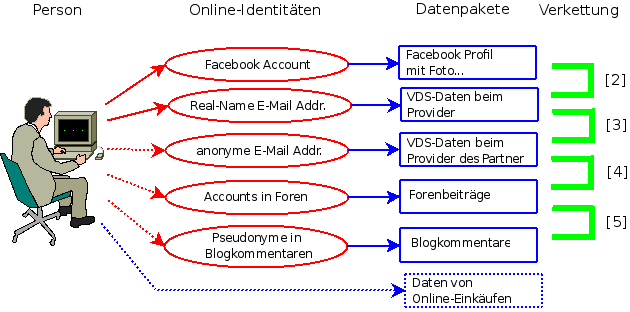
\includegraphics[scale=0.55]{../screenshots/nachdenken.png}
\caption{Datenverkettung}
\label{abb:nachdenken}
\end{center}
\end{figure}

Mit diesen Online-Identit�ten sind verschiedene Datenpakete verkn�pft, die irgendwo gespeichert und vielleicht nicht immer �ffentlich zug�nglich sind. Um �bersichtlich zu bleiben nur eine minimale Auswahl:
\begin{itemize}
 \item Das Facebook Profil enth�lt umfangreiche Daten: Fotos, Freundeskreis\dots
\item Bei der Nutzung von vielen Webdiensten fallen kleine Datenkr�mel an. Auch E-Mails werden von den Datensammlern ausgewertet. Die IP-Adresse des Absenders kann mit anderen Eintr�gen von Cookies oder User-Tracking-Systemen zeitlich korreliert werden und so k�nnen den Profilen die Mail-Adressen und reale Namen zugeordnet werden.
\item Von dem anonymen E-Mail Postfach findet man VDS-Daten bei den \underline{Empf�ngern} der E-Mails. Diese Datenpakete enthalten einen Zeitstempel sowie die IP-Adresse und E-Mail Adresse des Absenders und k�nnen mit weiteren Daten verkn�pft werden.
\item In Foren und Blogs findet man Postings und Kommentare, h�ufig mit den gleichen Pseudonymen, die auch f�r die E-Mail Adressen verwendet werden.
\item Online-Eink�ufern erforden in der Regel die Angaben zur Kontoverbindung und einer Lieferadresse, die der Person zugeordnet werden k�nnen.
\end{itemize}

\subsubsection*{Verkettung der Informationen und Datenp�ckchen}
Die verschiedenen Datenpakete k�nnen auf vielf�ltige Art verkn�pft werden. Diese \underline{Datenverkettung} ist eine neue Qualit�t f�r Angriffe auf die Privatsph�re, die untersch�tzt wird.

\begin{enumerate}
 \item Online Communities wie Facebook bieten viele M�glichkeiten. Neben der Auswertung von Freundschaftbeziehungen gibt es auch viele Fotos. Dieser Datenpool ist schon sehr umfangreich:
\begin{itemize}
 \item Wirtschaftswissenschaftler haben eine Methode vorgestellt, um Meinungsmacher und kreative K�pfe in Online-Communities zu identifizieren \footnote{ \href{http://www.heise.de/tp/r4/artikel/31/31691/1.html}{http://www.heise.de/tp/r4/artikel/31/31691/1.html}}.
\item MIT-Studenten erkennen homosexuelle Neigungen ihrer Kommilitonen anhand der Informationen �ber  Freundschaften in den Facebook-Profilen \footnote{ \href{http://www.heise.de/tp/r4/artikel/31/31181/1.html}{http://www.heise.de/tp/r4/artikel/31/31181/1.html}}.
\item Der Gr�nen-Vorsitzende �zdemir pflegte eine Freundschaft mit dem Intensivstraft�ter Muhlis Ari, ist in seinem Facebook-Profil erkennbar \footnote{ \href{http://www.heise.de/tp/r4/artikel/32/32138/1.html}{http://www.heise.de/tp/r4/artikel/32/32138/1.html}}.
\end{itemize}

\item Dem Facebook Profil kann man durch Kombination mit anderen Datenkr�meln den realen Namen und die meisten genutzten E-Mail Adressen zuordnen. Die Firma Rapleaf ist z.B. darauf spezialisiert. Auch pseudonyme Facebook Accounts k�nnen deanonymisiert werden.
\item Durch Analyse der im Rahmen der VDS gespeicherten IP-Adressen k�nnen bei zeitlicher �bereinstimmung beide E-Mail Adressen der gleichen Person zugeordnet werden. Ein einzelner passender Datensatz reicht aus. (Wenn nicht konsequent Anonymisierungsdienste f�r das anonyme Postfach verwendet werden.)
\item Die Verbindung zwischen anonymer E-Mail Adresse und Foren Account ergibt sich durch die Nutzung der E-Mail Adresse bei Anmeldung.
\item Durch Vergleiche von Aussagen und Wortwahl lassen sich Korrelationen zwischen verschiedenen Nicknamen in Foren und Blogs herstellen. Dem Autor sind solche Korrelationen schon mehrfach offensichtlich ins Auge gesprungen und konnten durch Nachfrage verifiziert werden.
\item Durch Datenschutzpannen k�nnen Informationen �ber Online-Eink�ufe mit anderen Daten verkn�pft werden. Dabei sch�tzt es auch nicht, wenn man sich auf das G�tesiegel des T�V S�d verl�sst und bei einem H�ndler einkauft, der bisher nicht negativ aufgefallen ist. Eine kleine Zusammenfassung vom 29.10.09 bis 04.11.09:
\begin{itemize}
 \item Die B�cher der Anderen (500.000 Rechnungen online einsehbar \footnote{ \href{http://www.netzpolitik.org/2009/exklusiv-die-buecher-der-anderen}{http://www.netzpolitik.org/2009/exklusiv-die-buecher-der-anderen}} )
\item Die Libris Shops (Zugang zu Bestellungen von 1000 Buchshops \footnote{ \href{http://www.netzpolitik.org/2009/exklusiv-die-libri-shops-der-anderen}{http://www.netzpolitik.org/2009/exklusiv-die-libri-shops-der-anderen}} )
\item Sparkassen-Shops (350.000 Rechnung online einsehbar \footnote{ \href{http://www.netzpolitik.org/2009/zugriff-auf-350-000-rechnungen-im-sparkasse-shop}{http://www.netzpolitik.org/2009/zugriff-auf-350-000-rechnungen-im-sparkasse-shop}} )
\item Acht Millionen Adressen von Quelle-Kunden sollen verkauft werden \footnote{ \href{http://www.zeit.de/digital/datenschutz/2009-11/quelle-kundendaten-verkauf}{http://www.zeit.de/digital/datenschutz/2009-11/quelle-kundendaten-verkauf}})
\end{itemize}
Eine reichhaltige Quelle f�r Datensammler, die Profile ihrer Zielpersonen vervollst�ndigen wollen oder nach potentiellen Zielpersonen rastern.
\end{enumerate}

Durch die Verkettung der Datenp�ckchen konnten in dem fiktiven Beispiel alle Online Identit�ten de-anonymsiert werden. F�r den Sammler, der diese Datensammlung in der Hand h�lt, ergibt sich ein komplexes Pers�nlichkeitsbild der Person P. Diese Datensammlung k�nnte das Leben von P in vielerlei Hinsicht beeinflussen, ohne dass dem Betroffenen klar wird, das hinter scheinbar zuf�lligen Ereignissen ohne Zusammenhang bewusste Entscheidungen stehen.
\begin{itemize}
 \item Die Datensammlungen werden mit kommerziellen Zielen ausgewertet, um uns zu manipulieren und unsere Kauf-Entscheidungen zu beeinflussen.
\item Personalabteilungen rastern routinem��ig das Internet nach Informationen �ber Bewerber. Dabei ist Google nur ein erster Ansatzpunkt. Bessere Ergebnisse liefern Personensuchmaschinen und soziale Netzwerke. Ein kurzer Auszug aus einem realen Bewerbungsgespr�ch:
\begin{itemize}
\item Personalchef: \textit{Es st�rt Sie sicher nicht, dass hier geraucht wird. Sie rauchen ja ebenfalls.}
\item Bewerber: \textit{Woher wissen Sie das?}
\item Personalchef: \textit{Die Fotos in ihrem Facebook-Profil \dots}
\end{itemize}
Qualifizierten Personalchefs ist dabei klar, dass eine kurze Recherche in Sozialen Netzen kein umfassendes Pers�nlichkeitsbild liefert. Die gefundenen Indizien k�nnen aber den Ausschlag f�r eine Ablehnung geben, wenn man als Frau gebrauchte Unterw�sche anbietet oder der Bewerber eine N�he zur Gothic-Szene erkennen l�sst.
\item Von der israelischen Armee ist bekannt, dass sie die Profile in sozialen Netzen �berpr�fen, wenn Frauen den Wehrdienst aus religi�sen Gr�nden verweigern. Zur Zeit verweigern in Israel 35\% der Frauen den Wehrdienst. Anhand der sozialen Netze wird der Lebenswandel dieser Frauen �berpr�ft. Es werden Urlaubsfotos in freiz�giger Bekleidung gesucht oder Anhaltspunkte f�r Essen in einem nicht-koscheren Restaurant. Auch aktiv wird dabei gehandelt und Fake-Einladungen zu einer Party w�hrend des Sabbats verschickt.
\item Firmen verschaffen sich unrechtm��ig Zugang zu Verbindungs- und Bankdaten, um ihrer Mitarbeiter auszuforschen. (Telekom- und Bahn-Skandal)
\item Identit�tsdiebstahl ist ein stark wachsendes Delikt. Kriminelle duchforsten das Web nach Informationen �ber reale Personen und nutzen diese Identit�ten f�r Straftaten. Wie sich Datenmissbrauch anf�hlt: Man wird pl�tzlich mit Mahnungen f�r nicht bezahlte Dienstleitungen �bersch�ttet, die man nie in Anspruch genommen hat
 \footnote{ \href{http://www.zeit.de/digital/datenschutz/2010-01/identitaetsdiebstahl-selbsterfahrung}{http://www.zeit.de/digital/datenschutz/2010-01/identitaetsdiebstahl-selbsterfahrung}}.
\item Mit dem Projekt INDECT hat die EU ein Forschungsprojekt gestartet und mit 14,8 Mio Euro ausgestattet, um unsere Daten-Spuren f�r Geheimdienste zu erschlie�en \footnote{ \href{http://www.zeit.de/digital/datenschutz/2009-09/indect-ueberwachung}{http://www.zeit.de/digital/datenschutz/2009-09/indect-ueberwachung}}.
\end{itemize}

\subsubsection*{Ich habe doch nichts zu verbergen\dots}
\dots oder habe ich nur zu wenig Fantasie, um mir die M�glichkeiten der Datensammler vorstellen, mein Leben zu beeinflussen?

\section{Ein Beispiel}
Das Seminar f�r angewandte Unsicherheit (SAU) hat ein sehr sch�nes Lehrbeispiel im Internet vorbereitet. Jeder kann nach Informationen dieser fiktiven Person selbst suchen und das Profil verifizieren. Es geht um folgende Person:
\begin{center}
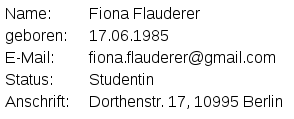
\includegraphics[scale=0.7]{../grafiken/beisp.png}
\end{center}
Diese Informationen k�nnte ein Personalchef einer Bewerbung entnehmen oder sie sind der Krankenkasse bekannt oder sie ist bei einer Demo aufgefallen\dots Eine kurze Suche bei Google und verschiedenen Personensuchmaschinen liefert nur sehr wenige Treffer, im Moment sind es 3 Treffer. Gleich wieder aufgeben?\\

Die moderne Studentin ist sozial vernetzt. Naheliegend ist es, die verschiedenen Netzwerke wie StudiVZ usw. nach F. abzusuchen. Bei Facebook wird man erstmals f�ndig. Es gibt ein Profil zu dieser Person mit Fotos, Interessen und (wichtig!) eine neue E-Mail Adresse:

\begin{center}

\includegraphics[scale=0.7]{../grafiken/beisp2.png}
\end{center}

Bezieht man diese Adresse in die Suche bei anderen Sozialen Netzwerken mit ein, wird man bei MySpace.com erneut f�ndig. Hier gibt es ein Profil mit dieser E-Mail Adresse und man findet den Twitter-Account von F. sowie ein weiteres Pseudonym:
\begin{center}

\includegraphics[scale=0.7]{../grafiken/beisp3.png}
\end{center}

Mit den beiden gefundenen Pseudonymen g.....17 und f.....85 kann man erneut bei Google suchen und die Ergebnisse mit den Informationen aus den Profilen zusammenfassen.
\begin{itemize}
\item g.....17 ist offenbar depressiv. Das verordnete Medikament deutet auf Angstzust�nde hin, wurde von der Patientin nicht genommen sondern ins Klo geworfen.
\item Sie hat Probleme im Studium und will sich krankschreiben lassen, um an Pr�fungen nicht teilnehmen zu m�ssen.
\item Au�erdem hat sie ein massives Alkohol-Problem und beteiligt sich am \textit{Syncron-Saufen} im Internet. Scheinbar ist sie auch vereinsamt.
\item F. ist offenbar lesbisch, sie sucht nach einer Frau bei abgefuckt.de.
\item F. ist im linksradikalen Spektrum aktiv. Sie hat an mehreren Demonstrationen teilgenommen und berichtet �ber  Erfahrungen mit Hausdurchsuchungen. M�glicherweise ist das die Ursache f�r ihre Angstzust�nde.
\item �ffentlich prangert sie in einem Diskussionsforum die Firma ihres Vaters an (wegen Ausspionierens von Mitarbeitern).
\item Ihre linksgerichtete Grundhaltung wird durch �ffentliche Unterst�tzung der Kampagne \textit{Laut ficken gegen Rechts} unterstrichen.
\item Von regelm��iger Arbeit h�lt sie nicht viel.
\item Die angebene Adresse ist falsch. F. wohnt in einer 11-Personen-WG in einem besetzten Haus in Alt-Moabit. Die WG sucht nach einem neuem Mitglied.
\item Die Wuschliste bei Amazon und Fotos bei Flickr\dots
\end{itemize}
 
W�rden sie als Personalchef diese fiktive Person einstellen?\\

Welche Ansatzpunkte erg�ben sich f�r den Verfassungsschutz?\\

Was k�nnte zuk�nftig f�r die Krankenkasse interessant sein?\\

Was h�tte F. tun k�nnen, um die Profilbildung zu vermeiden?

\subsubsection*{Bedeutung der Pseudonyme}
Die Suche nach Informationen �ber F. fiel relativ leicht. Sie verwendete die gleichen Pseudonyme mehrfach und die Pseudonyme waren eindeutig und einfach zu googeln. Damit ergeben sich viele Verkn�pfungen von einzelnen Informationsh�ppchen. Als Verteidigung gegen diese Recherche kann man viele unterschiedliche Pseudonyme verwenden oder zumindest schwer googelbare Pseudonyme, wenn man wieder�erkannt werden m�chte.\\

Die Wiedererkennbarkeit l�sst sich messen. Auf der Website \textit{How unique are your usernames?} \footnote{ \href{http://planete.inrialpes.fr/projects/how-unique-are-your-usernames/}{http://planete.inrialpes.fr/projects/how-unique-are-your-usernames}} kann man den Entropiewert seiner bevorzugten Pseudonyme berechnen lassen. Gute und schwer googelbare Pseudonyme haben Entropiewerte < 20. Werte �ber 40 sind sehr eindeutig und die damit verbunden Informationen somit leicht verkn�pfbar. 


\chapter{Spurenarm Surfen}
Das auf den folgenden Seiten vorgestellte Konzept zum spurenarmen Surfen umfasst folgende Punkte:

\begin{enumerate}
\item Die Nutzung datensammelnder Webangebote kann man vermeiden.
\item Die Annahme von Cookies und die Ausf�hrung von JavaScript wird auf vertrauensw�rdige Websites eingeschr�nkt.
\item Werbung, HTML-Wanzen und die Like-Buttons (mit denen Social Networks wie Facebook Daten sammeln) werden durch Filter blockiert.
\item Verr�terische Informationen des Browsers werden entfernt.
\item Risikoreiche und Privacy-unfreundliche Features wie PDF-Reader Plug-Ins, Browser History, Geolocation usw. werden im Browser deaktiviert.
\item HTTPS-Zertifikate werden zus�tzlich validiert, um Man-in-middle Angriffe zu erschweren.
\item Der Datenverkehr kann �ber einen Anonymisierungsdienst geleitet werden. Die verschl�sselte Kommunikation verhindert auch die Auswertung des Internetverkehrs durch mitlesende Dritte wie z.B. unsichere WLAN-Hotspots oder TK�V. (siehe \textit{Anonymymisierungsdienste nutzen})
\end{enumerate}

Mit diesen Ma�nahmen kann es vorkommen, dass Websites nicht wie erwartet funktionieren. Gute Webdesigner verzichteten auf suspekte Technologien, JavaScript wird sinnvoll eingesetzt und der Surfer auf fehlende Freigaben hingewiesen. Cookies sind meist f�r Logins n�tig und Javascript erm�glicht h�bsche Animationen oder Pr�fung von Eingaben.

\begin{center}

\includegraphics[scale=0.75]{../screenshots/cookies_required1.png}
\end{center}

Weniger gute Webseiten liefern seltsame Fehlermeldungen:

\begin{center}

\includegraphics[scale=0.75]{../screenshots/cookies_wrong1.png}
\end{center}

Ganz schlechte Websites machen irgendwas, aber nicht was man erwartet Gelegentlich werden auch Referer oder User-Agent ausgewertet, obwohl es belanglos sein sollte, und Surfer werden nicht auf die notwendigen Freigaben hingeweisen. Hier ist man auf Probieren und Raten angewiesen. Als erstes kann man Cookies freigeben. Wenn das hilft kann man Javascript gezielt f�r einzelne Server freigeben. Ob die Deaktivierung der Schutzma�nahmen die volle Funktionalit�t aufwiegt, muss man bei Bedarf selbst entscheiden.\\

\section{Auswahl des Webbrowsers}
Firefox ist der Webbrowser der Mozilla Foundation. Er ist kostenfrei nutzbar und steht auf der Website des Projektes \footnote{ \href{http://www.mozilla-europe.org/de/firefox}{http://www.mozilla-europe.org/de/firefox}} f�r fast alle Betriebssystem zum Download bereit. Linux-Distributionen enthalten den Browser in der Regel.\\

Debian GNU/Linux enth�lt eine branded version des Browsers unter dem Namen \textit{Iceweasel}, allerding oft in einer veralteten Version. Das Mozilla Debian Team stellt eine aktuelle Version in einem extra Repository \footnote{ \href{http://mozilla.debian.net}{http://mozilla.debian.net}} bereit.\\

Firefox kann durch viele von der Community entwickelte Add-ons und Anpassungen in der Konfiguration zu einem sicheren und privacy-freundlichen Browser aufgewertet werden. Ich beschr�nke mich im folgenden auf diesen einen Browser. Das ist schon sehr umfangreich, wenn man es gut machen will.

\subsubsection*{JonDoFox}
Der JonDoFox\footnote{ \href{https://www.anonym-surfen.de/jondofox.html}{https://www.anonym-surfen.de/jondofox.html}} ist ein Browser-Profil f�r Firefox, dass alle Einstellungen umsetzt, die auf den folgenden Seiten beschrieben werden. Nach der Installation von Mozilla Firefox ist das JonDoFox-Profil zus�tzlich zu installieren - fertig. Zuk�nftig fragt Firefox bei jedem Start, welches Profil genutzt werden soll. JonDoFox ist f�r anonymes Surfen mit JonDonym entwickelt worden, kann aber auch ohne Anonymisierungsdienst verwendet werden, indem man in der Statuszeile unten rechts auf \textit{Kein Proxy} oder \textit{Benutzerdefiniert} umschaltet.

\begin{center}
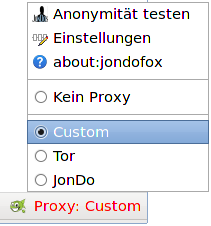
\includegraphics[scale=0.75]{../screenshots/jondofox-proxy-ohne.png}
\end{center}

Wenn man den Proxy \textit{Benutzerdefiniert} w�hlt, kann die User-Agent Kennung modifiziert werden. Das ist vor allem f�r Nutzer seltener Betriebssysteme sinnvoll, um sich in der Masse der Windows-Nutzer zu verstecken. In den Einstellungen des JonDoFox kann man f�r Benutzerdefinierte Proxys den \textit{Firefox 17.0 f�r Windows} (JonDo) oder \textit{Firefox 10.0 f�r Windows} (Tor) als Fake zu nutzen. Mit dieser kleinen Anpassung erh�lt man einen optimal konfigurierten Browser. Das folgende Kapitel kann man trotzdem lesen oder �berfliegen, um die damit verbundenen Einschr�nkungen besser zu verstehen.\\

\begin{figure}[htb]
\begin{center}
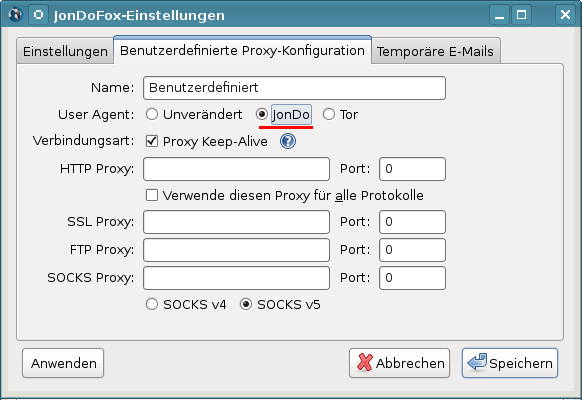
\includegraphics[scale=0.7]{../screenshots/jondofox-ua-ohne.png}
\caption{User-Agent Kennung konfigurieren}
\label{abb:jondofox-ua}
\end{center}
\end{figure}

Eine kurze Einf�hrung in den Umgang mit JonDoFox gibt es im Kapitel Anonymisierungsdienste.

\subsubsection*{JoDoBrowser}
Der JonDoBrowser\footnote{ \href{https://www.anonym-surfen.de/jondobrowser.html}{https://www.anonym-surfen.de/jondobrowser.html}} ist nicht nur sicher konfiguriert sondern enth�lt auch Modifikationen im Source Code von Mozilla Firefox, um eine h�here Anonymit�t zu bieten. Die aktuelle Beta Version arbeitet stabil und kann meiner Meinung nach f�r die t�gliche Arbeit eingesetzt werden.\\

Standardm��ig ist die Proxy-Umschaltung im JonDoBrowser deaktiviert. Das erweiterte Men� muss erst in den Einstellungen des JonDoFox-XPI (siehe Bild \ref{abb:proxyfreigeben}) aktiviert werden. Dann kann man wie beim JonDoFox auf \textit{``Kein Proxy``} umschalten und ohne Anonymisierungsdienst spurenarm surfen.

\begin{figure}[htb]
\begin{center}
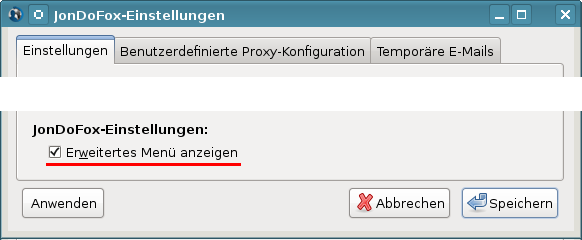
\includegraphics[scale=0.7]{../screenshots/jondobrowser-proxy-aktivieren.png}
\caption{Proxy-Umschaltung im JonDoBrowser freigeben}
\label{abb:proxyfreigeben}
\end{center}
\end{figure}
\section{Datensparsame Suchmaschinen}
Suchmaschinen werden sicher am h�ufigsten genutzt, um sich im Web zu orientieren. Neben den bekannten Datensammlern wie Google, MSN oder Yahoo gibt es durchaus Alternativen.\\

\subsubsection*{Suchmaschinen mit eigenem Index}
Es ist nicht einfach, eine Suchmaschine zu finden, die die Privatsph�re der Nutzer respektiert, einen umfangreichen Index zur Verf�gung stellt und gute Ergebnisse liefert. Ein paar Vorschl�ge:
\begin{itemize}
\item \textbf{DuckDuckGo.com} (\href{https://duckduckgo.com}{https://duckduckgo.com})\\
ist eine privacyfreundliche Suchmaschine. Es gibt sie in einer Java�script-freien Version (HTML) und mit Javascript. Wenn Javascript freigegeben ist, werden an der rechten Seite unter \textit{Search suggestions} Vorschl�ge f�r die Eingrenzung der Suche auf bestimmte Cluster angezeigt.\\

\begin{figure}[tb]
\begin{center}
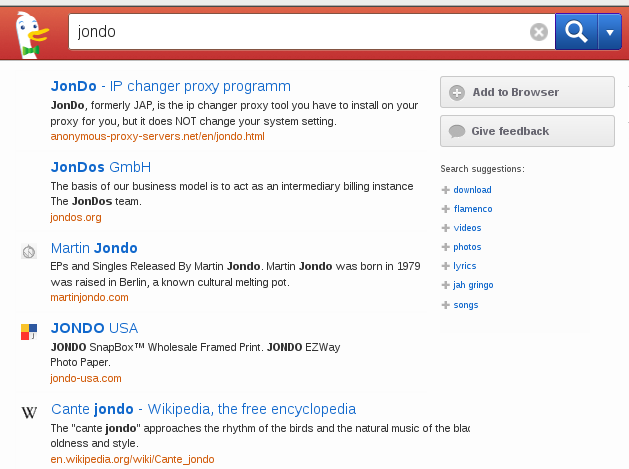
\includegraphics[scale=0.75]{../screenshots/duckduckgo.png}
\caption{Suchergebnisse bei DuckDuckGo mit Search suggestions}
\label{abb:ddgsuche}
\end{center}
\end{figure}

Bei der Suche nach ``jondo`` im Bild \ref{abb:ddgsuche} kann man bspw. die Ergebnisse auf Downloads begrenzen (wenn man nach dem Anonymierungs-Proxy sucht), auf Songs oder Lyrik (wenn man sich �ber den S�nger Martin JonDo informieren will) oder auf Flamenco (wenn man mehr Ergebnisse zum Cante jondo haben m�chte). Dieses Feature ist eine gute Kompensation f�r die nicht vorhandene Personalisierung.\\

Die Javascripte enthalten keinen Tracking Code. F�r diese Webseite kann ich die dauerhafte Freigabe von Javascript empfehlen.\\

Neben der eigentlichen Suche bietet DuckDuckGo viele nette Erweiterungen \footnote{ \href{https://duckduckgo.com/goodies.html}{https://duckduckgo.com/goodies.html}}. Das Suchfeld kann als Taschenrechner genutzt werden, Einheiten k�nnen umgerechnet werden, Fragen nach dem Wetter k�nnen beantwortet werden (in englisch: \textit{weather} oder \textit{is it raining})\dots u.v.a.m.

\item \textbf{Blekko} (\href{https://blekko.com/}{https://blekko.com})\\
Blekko hatte als erste Suchmaschine eine gute L�sung gegen Spam. Allerdings bietet sie keine Einschr�nkung auf bestimmte Sprachen. In den Ergebnissen dominieren englische Seiten. Die IP-Adressen der Nutzer werden nach 48h gel�scht.

\item \textbf{Open Directory} (\href{http://www.dmoz.de/}{http://www.dmoz.de} oder \href{http://www.dmoz.org/}{http://www.dmoz.org})\\
Das Open Directory ist ein Katalog, der von Freiwilligen gepflegt wird. Man kann die Suche auf Kategrien eingrenzen und erh�lt �bersichtliche Ergebnislisten.
\end{itemize}
Beide Suchmaschinen bieten gute Ergebnisse bei einfachen Suchanfragen. Komplexe Suchanfragen mit mehreren Begriffen beantwortet Google oder die als Google-Proxy nutzbaren Suchmaschine \textbf{Startpage} besser.

\subsubsection*{Meta-Suchmaschinen}
Meta-Suchmaschinen leiten die Suchanfrage an mehrere Suchdienste weiter. Sie sammeln die Ergebnisse ein und sortieren sie neu.
\begin{itemize}
 \item \textbf{Ixquick.com} (\href{https://www.ixquick.com/deu/}{https://www.ixquick.com/deu})\\
wird von der niederl�ndischen Firma Surfboard Holding B.V. betrieben. Die Suchmaschine speichert keine IP-Adressen und generiert keine Profile der Nutzer. Diese Meta-Suche fragt mehrere externe Suchmaschinen an, aber nicht Google. Ixquick.com ist mit dem Datenschutzsiegel EuroPriSe zertifiziert.\\

Als kleines Schmankerl bietet Ixquick die M�glichkeit, aus den Suchergebnissen heraus die Webseiten �ber einen anonymisierenden Proxy aufzurufen. Die aufgerufene Webseite sieht damit nur eine IP-Adresse von Ixquick. Neben den Ergebnissen findet man einen kleinen Link \textit{Proxy}: 
\begin{center}
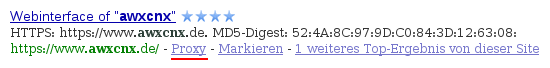
\includegraphics[scale=0.75]{../screenshots/ixquick.png}
\end{center}

Aus Sicherheitsgr�nden entfernt der Proxy Javascript Code aus den aufgerufenen Webseiten. Es ist daher m�glich, dass einige Webseiten nicht wie erwartet funktionieren. Au�erdem ist KEINE Eingabe von Daten in Textfeldern der aufgerufenen Webseite m�glich. Der Proxy kann die Webseiten nur darstellen.

\item \textbf{Startpage} (\href{https://startpage.com/}{https://startpage.com})\\
wird ebenfalls von Surfboard Holding B.V. betrieben und ist mit dem Datenschutzsiegel EuroPriSe zertifiziert. Die Suchmaschine bietet privacy-freundlichen Zugriff auf die Google-Suche, ist also einen ideale Erg�nzung zu Ixquick.com. Einen Proxy zum anonymen Aufruf der Webseiten aus den Ergebnissen bietet Startpage auch.

\item \textbf{Metager2.de} (\href{http://www.metager2.de/}{http://www.metager2.de})\\
ist ein Klassiker vom Suma e.V. Neben klassischen Suchdiensten wird auch die Peer-2-Peer Suche Yacy einbezogen. Dadurch verz�gert sich die Anzeige der Ergebnisse etwas.
\end{itemize}

\subsubsection*{Spezielle Anwendungsf�lle}
\begin{itemize}
 \item Wikipedia kann man auch ohne Umweg �ber Google direkt fragen, wenn man Informationen sucht, die in einer Enzyklop�die zu finden sind.
 \item Statt Google �bersetzen zu lassen, kann man LEO nutzen. Der Translator kennt neben Englisch und Deutsch weitere Sprachen.
\end{itemize}

\subsubsection*{Peer-2-Peer Suchmaschine}
Yacy \footnote{ \href{http://yacy.net/}{http://yacy.net}} ist eine zensurresistente Peer-2-Peer Suchmaschine. Jeder kann sich am Aufbau des Index beteiligen und die Software auf seinem Rechner installieren. Der Crawler ist in Java geschrieben, ben�tigt also eine Java-Runtime (JRE), die es f�r WINDOWS bei Oracle \footnote{ \href{http://java.sun.com}{http://java.sun.com}} zum kostenlosen Download gibt. Linuxer k�nnen das Paket \textit{default-jre} mit der Softwareverwaltung installieren. Danach holt man sich die Yacy-Software von der Website des Projektes und startet den Installer - fertig. F�r Debian, Ubuntu und Linux Mint bietet das Projekt ein Repository  \footnote{ \href{http://www.yacy-websuche.de/wiki/index.php/De:DebianInstall}{http://www.yacy-websuche.de/wiki/index.php/De:DebianInstall}} mit fertigen Paketen.\\

Nach dem Start von Yacy kann man im sich �ffnenden Bowserfenster die Basiskonfiguration anpassen und los gehts. Die Suchseite ist im Browser unter \href{http://localhost:8080}{http://localhost:8080} erreichbar.\\

Die Beantwortung der Suchanfragen dauert mit 5-10sec ungewohnt lange. Au�erdem muss Javascript f�r \textit{http://localhost} freigegeben werden, damit die Ergebisseite sauber dargestellt wird. Mit den Topwords unter den Ergebnissen bietet Yacy ein Konzept, um die Suchanfrage zu pr�zisieren.\\

F�r alle alternativen Suchmaschinen gilt, dass sie eine andere Sicht auf das Web bieten und die Ergebnisse sich von Google unterscheiden. Man sollte bei der Beurteilung der Ergebnisse beachten, dass auch Google nicht die reine Wahrheit bieten kann, sondern nur eine bestimmte Sicht auf das Web.

\subsubsection*{Google ???}
Anfang Februar 2012 hat Google seine Suchmaschine �berarbeitet. Die Webseite macht jetzt intensiven Gebrauch von Javascript. Eine vollst�ndige Analyse der verwendeten Sch�ffel�techniken liegt noch nicht vor. Einige vorl�ufige Ergebnisse sollen kurz vorgestellt werden:

\begin{description}
 \item[Einsatz von EverCookies:] Der Surfer wird mit EverCookie Techniken markiert. Die Markierung wird im DOMStorage gespeichert. Der DOMStorage wurde vom W3C spezifiziert, um Web-Applikationen die lokale Speicherung gr��erer Datenmengen zu erm�glichen und damit neue Features zu erschlie�en. Google wertet die User-Agent Kennung und weitere Informationen �ber den Browser aus, um die M�glichkeit der Nutzung des DOMStorage erst einmal zu pr�fen und gegebenenfalls Alternativen wie normale Cookies zu verwenden.

\item[Tracking der Klicks auf Suchergebnisse:] Bei Klick auf einen Link in den Suchergebnissen wird die Ziel-URL umgeschrieben. Aus der f�r den Surfer sichtbaren Zieladresse 
\begin{verbatim}
  https://www.awxcnx.de/handbuch.htm 
\end{verbatim} 

wird im Moment des Klick eine Google-URL: 
\begin{verbatim}
  http://www.google.de/url?q=https://www.awxcnx.de/...... 
\end{verbatim} 

Die zwischengeschaltete Seite enth�lt eine 302-Weiterleitung auf die urspr�ngliche Ziel-URL. Der Surfer wird also fast unbemerkt �ber einen Google-Server geleitet, wo der Klick registriert wird. (Bei deaktiviertem Javascript ist stets die Google-URL sichtbar, nicht die Zieladresse.)\\

Diese Umschreibung der Links gibt es auch bei Bing, Facebook, Youtube und anderen Daten�sammlern. Das Firefox Add-on Google Privacy kann diese Umschreibung verhindern. Das Add-on ist noch im Beta Status. Die Entwicklung von \textit{Google Privacy} ist ein Wettlauf zwischen Hase und Igel. Einfacher und sicherer ist es, privacy freundliche Suchmaschinen zu nutzen.

\item[Browser Fingerprinting:] Mittels Javascript wird die innere Gr��e des Browserfensters ermittelt. Folgenden Code findet man in den Scripten:
\begin{verbatim}
 I[cb].oc= function() {
 var a=0, b=0;
 self.innerHeight?(a=self.innerWidth,b=self.innerHeight):....;
 return {width:a, height:b}
 };
\end{verbatim} 

Die ermittelten Werten werden als Parameter \textit{biw} und \textit{bih} in der Google-URL �bergeben. Sie haben aber keinen Einfluss auch die Bildschirmdarstellung. Auch wenn das Browserfenster zu klein ist und die Darstellung nicht passt, bleiben die festen Gr��en der HTML-Elemente erhalten.\\

Die inneren Abmessungen des Browserfensters sind sehr individuelle Parameter, der von Betriebssystem und gew�hlten Desktop-Einstellungen abh�ngig sind. Sie werden von der Schriftgr��e in der Men�leiste, der Fensterdekoration, den aktivierten Toolbars der Desktops bzw. der Browser usw. beeinflusst. Sie sind f�r die Berechnung eines individuellen Fingerprint des Browsers gut geeigent. Anhand des Browser-Fingerprint k�nnen Surfer auch ohne Cookies oder EverCookies wiedererkannt werden. Die Google Technik kann dabei besser differenzieren als das Projekt Panopticlick der EFF, das berets 80\% der Surfer eindeutig identifizieren konnte.
 \end{description}

Auf der Webseite der Google-Suche kann man dem Tracking kaum entgehen. Wer unbedingt die Ergebnisse von Google braucht, kann die Suchmaschine \textit{Startpage.com} als anonymisierenden Proxy nutzen. Sie ist mit dem Datenschutzsiegel EuroPriSe zertifiziert. Andere Suchmaschinen bieten eine andere Sicht auf das Netz - auch nicht schlecht, erfordert aber etwas Umgew�hnung.



\subsection{Firefox konfigurieren}
Am einfachsten installiert man ein Plug-In f�r die Suchleiste von Firefox, indem man die Web�seite der Suchmaschine aufruft und die Liste der Suchmaschinen ausklappt. Am Ende der Liste findet man das Plug-In f�r diese Suchmaschine, das man mit einem Klick hinzuf�gen kann.\\
\begin{figure}[tb]
\begin{center}
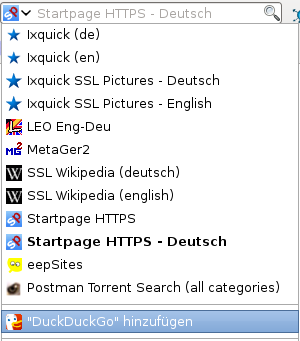
\includegraphics[scale=0.75]{../screenshots/suchmaschine-install.png}
\caption{Suchmaschine DuckDuckGo hinzuf�gen}
\label{abb:ffsucheadd}
\end{center}
\end{figure}

F�r viele Suchdienste gibt es Plug-Ins zur Integration in die Suchleiste von Mozilla Firefox bei mycroft.mozdev.org\footnote{ \href{http://mycroft.mozdev.org/}{http://mycroft.mozdev.org/}}. In einem Suchformular gibt man den Namens der Suchmaschine ein und findet schnell ein umfangreiche Liste von Varianten. Ein Klick in der Liste der Ergebnisse installiert das Plug-In in der Suchleiste. (Die Installation funktioniert nur mit JavaScript.)\\

F�r viele Suchmaschinen wie DuckDuckGo, Ixquick, Google, Wikipeadia, Startingpage u.a.m. gibt es eine Variante mit SSL-Verschl�sselung. Diese Variante sollte bevorzugt werden.\\

Au�erdem kann die Generierung von Suchvorschl�gen deaktiviert werden. Die Vorschl�ge kommen von dem gew�hlten Suchdienst, verlangsamen aber die Reaktion auf Eingaben deutlich. Ich weiss selber, was ich suche!  Den Dialog findet man unter \textit{Suchmaschinen verwalten} in  der Liste der Suchmaschinen.

\begin{figure}[tb]
\begin{center}
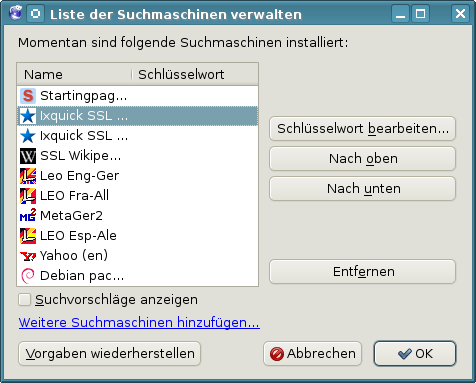
\includegraphics[scale=0.75]{../screenshots/firefox_suche.png}
\caption{Suchmaschinen verwalten}
\label{abb:ffsuche}
\end{center}
\end{figure}

\section{Cookies}
Cookies werden f�r die Identifizierung des Surfers genutzt. Neben der erw�nschten Identifizierung um personalisierte Inhalte zu nutzen, beispielsweise einen Web-Mail-Account oder um Eink�ufe abzuwickeln, werden sie auch f�r das Tracking von Nutzern verwendet.\\

Der Screenshot Bild \ref{abb:cookiespiegel} zeigt die Liste der Cookies, die bei einem einmaligen Aufruf der Seite \textit{www.spiegel.de} gesetzt wurden. Neben den Cookies von \textit{spiegel.de} zur Z�hlung der Leser setzen gleich mehrere datensammelnde Werbeserver Cookies und au�erdem Z�hldienste (quality-chanel.de, ivwbox.de), welche die Reichweiten von Online-Publikationen auswerten.\\

\begin{figure}[p]
\begin{center}
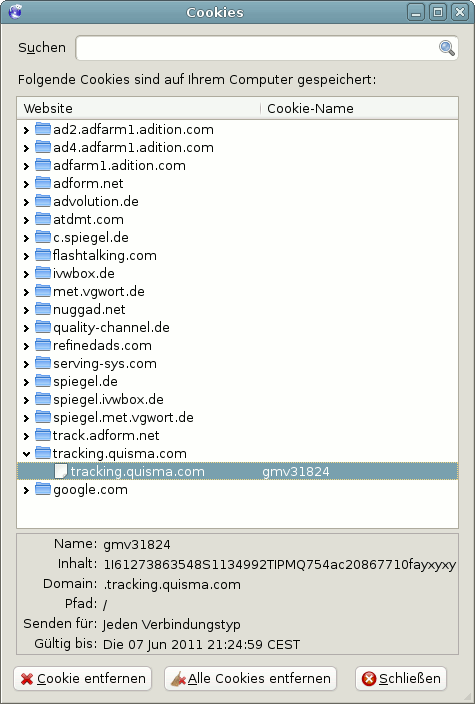
\includegraphics[scale=0.75]{../screenshots/cookies_spiegel.png}
\caption{Liste der Cookies beim Besuch von Spiegel-Online}
\label{abb:cookiespiegel}
\end{center}
\end{figure}

Es ist nicht ungew�hnlich, dass popul�re Webseiten mehrere Datensammler einbinden. Eine Studie der Universit�t Berkeley \footnote{ \href{http://heise.de/-1288914}{http://heise.de/-1288914}}  hat 2011 beim Surfen auf den TOP100 Webseiten 5.675 Cookies gefunden (ohne Login oder Bestellung). 4.914 Cookies wurden von Dritten gesetzt, also nicht von der aufgerufenen Webseite. Die Daten wurden an mehr als 600 Server �bermittelt. Spitzenreiter unter den Datensammlern ist Google, 97\% der popul�ren Webseiten setzen Google-Cookies.\\

Sinnvoll ist ein \textbf{Whitelisting} f�r die Behandlung von Cookies:

\begin{enumerate}
\item Standardm��ig wird die Annahme von Cookies verweigert.
\item F�r vertrauensw�rdige Websites, welche die Nutzung von Cookies zur Erreichung der vollen Funktion ben�tigen, werden Ausnahmen zugelassen.
\item Die f�r den Zugriff auf personalisierte Inhalte gespeicherten Cookies sollten beim Schlie�en des Browsers automatisch gel�scht werden. Einige Websites verwenden diese Cookies auch nach dem Logout f�r das User-Tracking.
\end{enumerate} 

Fast alle Login-Seiten, welche Cookies zur Identifizierung des Surfers verwenden, weisen mit einem kleinen Satz auf die notwendigen Freigaben hin. Treten beim Login seltsame Fehler auf, z.B. st�ndig die Fehlermeldung \textit{FALSCHES PASSWORT}, verweigert der Browser wahrscheinlich die Annahme von Cookies. Die Website sollte in die Liste der vertrauensw�rdigen Websites aufgenommen werden.\\



\subsection{Mozilla Firefox konfigurieren}
Mozilla Firefox bietet bereits standardm��ig die M�glichkeit, die meisten Cookies ohne Einbu�en am Surf-Erlebnis loszuwerden. Im Bild \ref{abb:cookiesff} gezeigte Dialog \textit{Einstellungen} Sektion \textit{Datenschutz} kann die Annahme von Fremd-Cookies standardm��ig deaktiviert werden.\\

\begin{figure}[htb]
\begin{center}
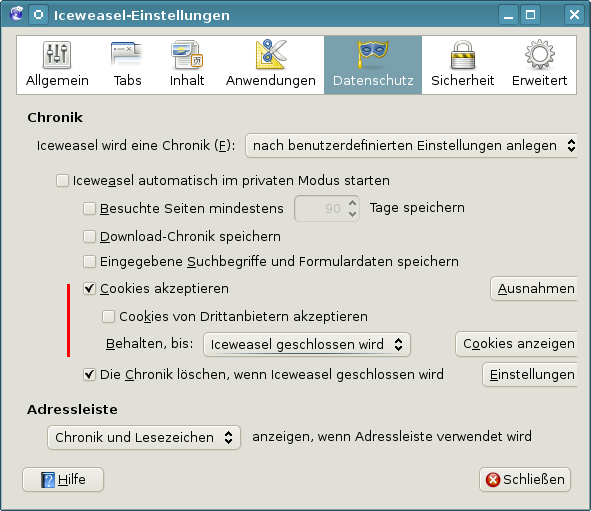
\includegraphics[scale=0.75]{../screenshots/CookiesFF.png}
\caption{Cookies-Einstellungen in Firefox}
\label{abb:cookiesff}
\end{center}
\end{figure}

Mit einem Klick auf den Button \textit{Ausnahmen} kann man Server konfigurieren, die Cookies setzen d�rfen oder grunds�tzlich blockiert werden. Um von Google nicht beim Besuch der meisten deutschen Websites verfolgt zu werden, ist es n�tig, diesen Dienst ausdr�cklich zu blockieren.\\

Anderenfalls wird der Browser beim Start durch den Aufruf der Default-Seite oder beim Laden der Phishing-Datenbank mit einem Google-Cookie ``personalisiert''. Durch eingebettete Werbung und Google-Analytics auf vielen Websites kann Google unbedarfte Surfer effektiv beobachten.

\subsubsection*{Zus�tzliche Add-ons f�r Firefox}
Die Firefox Addon Sammlung bietet viele Add-ons um die Verwaltung von Cookies zu erleichtern. Nicht alle werden noch gepflegt und sind mit aktuellen Versionen von Firefox kompatibel. Das Add-on \textbf{CookieMonster} \footnote{ \href{https://addons.mozilla.org/de/firefox/addon/cookie-monster/}{https://addons.mozilla.org/de/firefox/addon/cookie-monster/}} ist empfehlenswert. Es erlaubt die site-spezifische Verwaltung von Cookies.\\

Ein einfacher Klick auf das Install-Symbol der Website startet den Download der Erweiterung und installiert sie. Nach dem Neustart von Firefox ist in der Statusleiste ein zus�tzliches Symbol vorhanden. Ein Klick mit der linken(!) Maustaste auf das blau-schwarze ``CM`` �ffnet das in Bild \ref{abb:cookiesafe_1} dargestellte Men� (nur wenn die Website Cookies nutzen m�chte).

\begin{figure}[htb]
\begin{center}
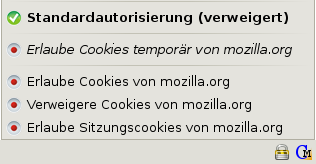
\includegraphics[scale=0.75]{../screenshots/Cookies1.png}
\caption{CookieMonster Men�}
\label{abb:cookiesafe_1}
\end{center}
\end{figure}

\begin{description}
\item[Erlaube Cookies tempor�r] erlaubt es dem aktuellen Server, nur f�r diese Sitzung Cookies zu setzen. Mit dem Schlie�en des Browsers werden die Cookies und die Ausnahme�reglung gel�scht.
\item[Erlaube Cookies] erlaubt es dem aktuellen Server, unbegrenzt g�ltige Cookies zu setzen. Diese Variante wird nur ben�tigt, wenn man bei einem sp�teren Besuch der Website automatisch wieder angemeldet werden m�chte.
\item[Verweigere Cookies] erlaubt es dem aktuellen Server nicht, Cookies zu setzen.
\item[Erlaube Sessioncookies] erlaubt es dem aktuellen Server, Cookies zu setzen. Mit dem Schlie�en des Browsers werden diese Cookies wieder gel�scht. Bei folgenden Besuchen d�rfen wieder neue Cookies gesetzt werden.
\end{description}

Nach der Installation von CookieMonster muss man das Standardverhalten auf \textit{Alle Cookies blockieren} umschalten. Das ist sicherer, als nur die Cookies von Dritt-Seiten zu blockieren. Die Einstellungen werden im Add-ons-Manager unter \textit{Extras -> Add-ons} in der Sektion \textit{Erweiterungen} konfiguriert.

\begin{figure}[htb]
\begin{center}
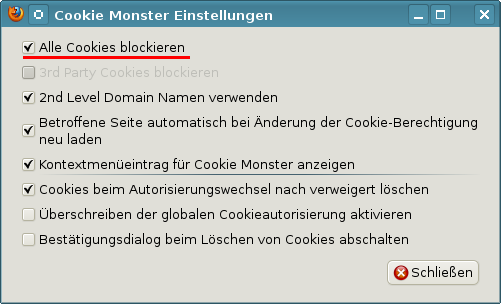
\includegraphics[scale=0.75]{../screenshots/CookiesFF2.png}
\caption{CookieMonster Einstellungen}
\label{abb:cookiesafe_2}
\end{center}
\end{figure}

\subsection{Super-Cookies in Firefox}
Mozilla Firefox bietet auch die clientseitige Datenspeicherung. Dieser DOM-Storage oder Web-Storage wird gelegentlich auch als Super-Cookie bezeichnet, da bis zu 5 MB gro�e Datenmengen mit Hilfe von Javascript abgelegt werden k�nnen.\\

Aktuelle Versionen von Firefox wenden die Beschr�nkungen f�r Cookies auch auf den DOMStorage an. Es reicht aus, die Cookies zu deaktivieren. Damit ist auch die clientseitige Datenspeicherung deaktiviert.\\

Diese parallele Anwendung der Einstellung f�r Cookies auf DOMStorage gilt nur f�r Firefox. Andere Browser verhalten sich bez�glich der clientseitigen Datenspeicherung anders! Bei Opera habe ich noch keine M�glichkeit gefunden, die lokale Speicherung von Daten gezielt zu deaktivieren.\\

\subsection{Flash-Cookies verwalten}
Auch Flash-Applikationen k�nnen Cookies setzen, sogenannte \textit{Local Shared Objects (LSO)}. Diese Datenkr�mel k�nnen bis zu 100kByte Daten fassen und ignorieren die Einstellungen des Browsers. Sie werden neben der Speicherung von Einstellungen auch zum Nutzertracking verwendet von Youtube, Ebay, Hulu...\\

Aktuelle Browser (mit Ausnahme von Opera) verwalten die Flash-Cookies nach den gleichen Regeln wie normale Cookies. Zus�tzliche Add-ons zum L�schen der Flash Cookies sind nicht mehr n�tig. Au�erdem bieten Flash-Player unterschiedliche M�glichkeiten, diese Datenspeicherung zu deaktivieren:
\begin{enumerate}
\item Wer den \textbf{Adobe Flash-Player} nutzt, kann mit einer Flash-Anwendung auf der Webseite von Macromedia \footnote{ \href{http://www.macromedia.com/support/documentation/ de/flashplayer/help/settings\_manager.html}{http://www.macromedia.com/support/documentation/ de/flashplayer/help/settings\_manager.html}} die Einstellungen f�r das Speichern und Auslesen von Informationen sowie Nutzung von Mikrofon und Kamera anpassen.\\

Auf der Seite \textit{Globale Speicher�einstellungen} ist die Datenspeicherung zu deaktivieren (Bild \ref{abb:flashplayer}). Anschlie�end sind auf der Seite \textit{Webseiten Speichereinstellungen} die bisher gespeicherten Cookies zu l�schen.\\

\begin{figure}[htb]
\begin{center}
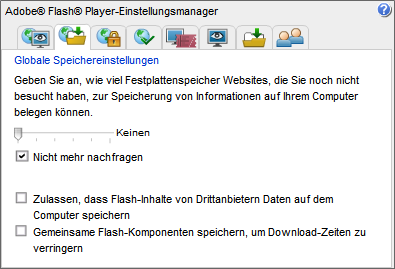
\includegraphics[scale=0.55]{../screenshots/flash1.png}
\caption{Einstellungsmanager f�r Adobe Flash-Player}
\label{abb:flashplayer}
\end{center}
\end{figure}

Wer das Add-on NoScript nutzt, muss zus�tzlich zur aktuellen Webseite dem Server \textit{wwwimages.adobe.com} das Ausf�hren von Javascript erlauben. Anderenfalls funktioniert die Flash-Applikation nicht.
\item Der freie Flash-Player \textbf{Gnash} bietet die M�glichkeit, die Speicherung von Cookies zu konfigurieren. Man klickt mit der rechten Maustaste auf ein Flash-Movie und w�hlt den Punkt \textit{Bearbeiten - Einstellungen} im Kontextmen� und schickt man alle Shared Objects nach /dev/null.

\end{enumerate}


\section{EverCookies}
80\% der Internetnutzer lehnen das Tracking ihres Surfverhaltens ab. Viele Surfer ergreifen einfache Ma�nahmen gegen Tracking Cookies. Nach einer Untersuchung von AdTiger blockieren 52,5\% der Surfer die Annahme von Cookies, die nicht von der aufgerufenen Website stammen (sogenannte Third-Party-Cookies). Andere Studien \footnote{ \href{http://smorgasbork.com/component/content/article/84-a-study-of-internet-users-cookie-and-javascript-settings}{http://smorgasbork.com/component/content/article/84-a-study-of-internet-users-cookie-and-javascript-settings}} kommen auf 15\%...35\% Cookie-Verweigerer unter den Surfern (was mir seri�ser erscheint). Dabei handelt es meist um Surfer, die regelm��ig auf dem Datenhighway unterwegs sind und somit die Erstellung pr�ziser Profile erm�glichen k�nnten. Von Gelegenheits-Surfern kann man kaum umfassenden Interessen-Profile erstellen.\\ 

Die Tracking-Branche reagiert auf diese Entwicklung mit erweiterten Markierungen, die unter der Bezeichnung \textit{EverCookie} zusammengefasst werden. Zus�tzlich zum Tracking-Cookie werden weitere Markierungen im Browser gespeichert. Sp�ter kann ein gel�schtes Tracking-Cookie anhand dieser Markierungen wiederhergestellt werden.\\

Nach empirischen Untersuchungen der University of California \footnote{ \href{http://www.law.berkeley.edu/privacycensus.htm}{http://www.law.berkeley.edu/privacycensus.htm}} nutzen viele Tracking�dienste EverCookie Techniken. H�ufig werden seit 2005 Flash-Cookies bzw. LSOs parallel zu normalen Cookies eingesetzt, wobei diese Technik auf dem absteigenden Ast ist. 2011 nutzen 37\% der TOP100 Webseiten diese Technik, 2012 nur noch 17\%. Die Flash-Cookies werden durch HTML5-Speichertechniken wie DOMstorage ersetzt und ETags. 31\% der TOP100 Webseiten nutzen moderne HTML5-Techniken zur Markierung der Surfer (Stand 2012). 
\begin{itemize}
\item Die \textit{Google-Suche} nutzt DOMstorage, was eine Markierung von Nutzern auch bei deaktivierten Cookies erm�glicht.
\item Die Firma \textit{Clearspring} protzt damit, pr�zise Daten von 250 Mio. Internetnutzern zu haben. Sie setzte bis 2010 Flash-Cookies ein, um gel�schte Cookies wiederherzustellen.
\item \textit{Ebay.de} verwendet Flash-Cookies, um den Browser zu markieren.
\item \textit{AdTiger.de} bietet umfangreiche Angebote zur gezielten Ansprache von Surfern und protzt damit, 98\% der Zugriffe �ber einen Zeitraum von deutlich l�nger als 24h eindeutig einzelnen Nutzern zuordnen zu k�nnen. Nach einer eigenen Studie kann AdTiger aber nur bei 47,5\% der Surfer normale Cookies setzen.
\item Die Firma \textit{KISSmetrics} (\textit{``a revolutionary person-based analytics platform``}) setzte zus�tzlich zu Cookies und Flash-Cookies noch ETags aus dem Cache, DOMStorage und IE-userData ein, um Surfer zu markieren. Aufgrund der negativen Schlagzeilen wird seit Sommer 2011 auf den Einsatz von ETags verzichtet.
\end{itemize}

\subsubsection*{EverCookies - never forget}
Der polnische Informatiker Samy Kamkar hat eine Demonstration \footnote{ \href{http://samy.pl/evercookie/}{http://samy.pl/evercookie/}} von EverCookie Techniken erstellt, die verschiedene technische M�glichkeiten basierend auf HTML5 zeigen:
\begin{itemize}
\item Local Shared Objects (Flash Cookies)
\item Silverlight Isolated Storage
\item Cookies in RGB Werten von automatisch generierten Bildern speichern
\item Cookies in der History speichern
\item Cookies in HTTP ETags speichern
\item Cookies in Browser Cache speichern
\item window.name auswerten
\item Internet Explorer userData Storage
\item Internet Explorer userData Storage
\item HTML5 Database Storage via SQLite
\item HTTP-Auth speichern (zuk�nftig)
\end{itemize}

\subsubsection*{Verteidigungsstrategien}
Zur Verteidigung gibt es drei M�glichkeiten:
\begin{enumerate}
\item Die Verbindung zu Tracking-Diensten kann mit \textbf{AdBlockern} komplett verhindert werden. Es sind Filterlisten zu nutzen, die in der Regel als Privacy Listen bezeichnet werden.
\item Viele EverCookie Techniken nutzen Javascript. Die \textbf{Freigabe von Javascript} nur auf wenigen, vertrauensw�rdigen Seiten sch�tzt ebenfalls.
\item Ein EverCookie-sicherer Browser kann nur mit Konfigurationseinstellungen nicht erreicht werden. Der Datenverkehr ist durch zus�tzliche Ma�nahmen zu reinigen. Bisher kann nur der \textbf{JonDoFox} und der \textbf{JonDoBrowser} alle von Samy Kamkar vorgestellten Techniken w�hrend des Surfens blockieren.
\item Der \textbf{TorBrowser} beseitigt alle Markierungen beim Beenden der Surf-Session (Schlie�en des Browsers oder \textit{Neue Identit�t} im TorButton w�hlen). W�hrend der Session ist man anhand von EverCookies wiedererkennbar. Dieses Verhalten entspricht der Zielstellung der Tor-Entwickler. 
\end{enumerate}

\section{JavaScript}
JavaScript ist eine der Kerntechniken des modernen Internet, birgt aber auch einige Sicherheitsrisiken.
\begin{enumerate}
\item Mit Hilfe von Javascript kann man ein Vielzahl von Informationen �ber den Browser und das Betriebssystem auslesen. Bildschirmgr��e, Farbeinstellungen, installierte Plugins und Hilfs-Applikationen.... Die Website \href{http://browserspy.dk}{http://browserspy.dk} zeigt eine umfangreiche Liste.\\

Diese Informationen k�nnen zu einem individuellen Fingerabdruck verrechnet werden. Anhand dieses Fingerabdruck kann der Surfer wiedererkannt werden, auch wenn er die IP-Adresse mit VPNs oder Anonymisierungsdiensten verschleiert. Die EFF geht davon aus, dass diese Methode von vielen Datensammlern genutzt wird.
\begin{itemize}
 \item \textit{Yahoo! Web Analytics} nutzt Javascript Tracking Code, wenn Cookies blockiert werden.
 \begin{quote}
  \textit{In case Yahoo! Web Analytics cannot set a cookie, the system can still retrieve information from the JavaScript tracking code, the IP address and the web browser user agent. \footnote{ \href{http://help.yahoo.com/l/us/yahoo/ywa/documentation/install\_guide/ig\_get\_started.html}{http://help.yahoo.com/l/us/yahoo/ywa/documentation/install\_guide/ig\_get\_started.html}} }
 \end{quote}  
 \item Ein weiteres Beispiel ist die Firma \textit{bluecave} \footnote{ \href{http://www.bluecava.com}{http://www.bluecava.com}}. Das Trackingscript \textit{BCAL5.js} sammelt Informationen zur verwendeten Software, installierte Schriftarten, Bildschirmgr��e, Browser Plug-ins und ein paar mehr Daten, um daraus einen individuellen Fingerprint zu berechnen. \textit{bluecave} protzt damit, 99\% der Surfer zu erkennen.
 \item Der Trackingdienst Multicounter \footnote{ \href{http://www.multicounter.de/features.html}{http://www.multicounter.de/features.html}} und die Google Suche speichern die per Javascript ausgelesene Bild�schirm�gr��e als individuelles Merkmal.
\end{itemize}

\item Einige EverCookie Techniken nutzen Javascript, um zus�tzliche Markierungen im Browser zu hinterlegen und gel�schte Tracking Cookies wiederherzustellen.

\item Durch Einschleusen von Schadcode k�nnen Sicherheitsl�cken ausgenutzt und der der Rechner kann kompromittiert werden. Das Einschleusen von Schadcode erfolgt dabei auch �ber vertrauensw�rdige Webseiten, beispielsweise mit Cross Site Scripting, wenn diese Websites nachl�ssig programmiert wurden. Werbebanner k�nnen ebenfalls b�s�artigen Javascriptcode transportieren. Im Januar 2013 lieferten die Server des Werbe�netzwerkes OpenX Scripte aus, die Rechner durch Ausnutzung mehrerer Sicherheitsl�cken im Internet Explorer kompromittierten.\footnote{ \href{http://heise.de/-1787511}{http://heise.de/-1787511}}
\end{enumerate}

Ein generelles Abschalten ist heutzutage nicht sinnvoll. �hnlich dem Cookie-Management ben�tigt man ein Whitelisting, welches JavaScript f�r vertrauensw�rdige Websites zur Erreichung der vollen Funktionalit�t erlaubt, im allgemeinen jedoch deaktiviert. Gute Webdesigner weisen den Nutzer darauf hin, dass ohne Javascript eine deutliche Einschr�nkung der Funktionalit�t zu erwarten ist. 



\subsection{NoScript f�r Mozilla Firefox}
Die Einstellungen f�r JavaScript lassen sich mit dem Add-on \textit{NoScript} komfortabel verwalten. Die Erweiterung kann von der Website \footnote{ \href{https://addons.mozilla.org/de/firefox/addon/noscript/}{https://addons.mozilla.org/de/firefox/addon/noscript}} installiert werden. Ein einfacher Klick auf das Download-Symbol startet die Installation. Im Anschluss ist Firefox neu zu starten.\\

\begin{figure}[htb]
\begin{center}
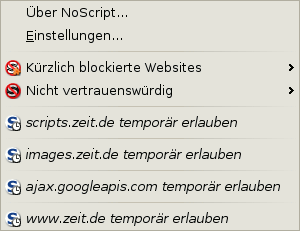
\includegraphics[scale=0.75]{../screenshots/noscript_allow.png}
\caption{NoScript-Button und Men� in der Statuszeile}
\label{abb:noscript_button}
\end{center}
\end{figure}

Nach dem Neustart von Firefox ist in der Statusleiste ein zus�tzliches Symbol vorhanden, welches den Status der Freigabe von JavaScript anzeigt. Ein Klick auf das Symbol �ffnet das im Bild \ref{abb:noscript_button} gezeigte Men�, welches JavaScript f�r die aktuellen Sites generell oder nur tempor�r freigibt.\\

Einige Webseiten verwenden \textit{Captchas} als Spamschutz. Die Captchas werden von Drittseiten eingebunden (Recaptcha.com, Nucaptcha.com...) und funktionieren nur, wenn Javascript f�r den Captcha-Provider freigegeben ist. Wenn das Captcha auf einer Webseite nicht funktioniert, schauen sie in der NoScript-Liste nach, ob evtl. ein Captcha-Provider dabei ist und geben sie Javascript tempor�r f�r diese Domain frei.\\

Weitere Skripte von Drittanbietern werden �blicherweise nur zum Spionieren verwendet und sind f�r die Funktionalit�t selten notwendig.\\

W�hlt man den Punkt \textit{Einstellungen} im NoScript-Men�, �ffnet sich der Einstellungsdialog (Bild \ref{abb:noscript_einst}), der auf dem Reiter \textit{Positivliste} eine Liste der Websites zeigt, f�r welche Java-Script freigegeben wurde. Als Erstes sollte man aus der Positivliste alles entfernen, was man nicht wirklich braucht. In der Liste findet man standardm��ig mit \textit{googlesyndications} auch Surf-Tracker.\\

\begin{figure}[htb]
\begin{center}
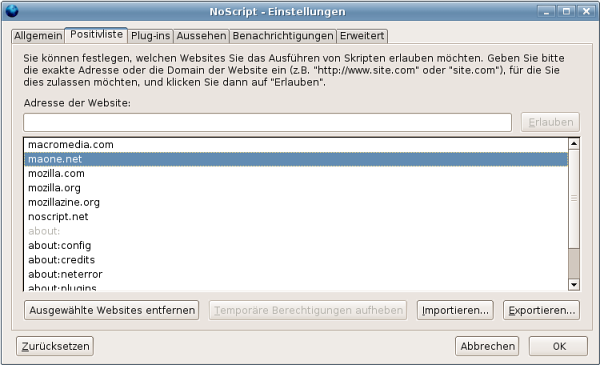
\includegraphics[scale=0.58]{../screenshots/noscript_einst.png}
\caption{Einstellungen f�r NoScript}
\label{abb:noscript_einst}
\end{center}
\end{figure}

Auf dem Reiter \textit{Benachrichtigungen} l�sst sich beispielsweise konfigurieren, ob NoScript den Surfer mit einem Sound oder mit einem Info-Balken dar�ber informiert, dass Scripte auf der aktuellen Webseite blockiert wurden.\\

Der Sound nervt mich, diese Option habe ich deaktiviert. Wenn eine Webseite jedoch nicht wie erwartet funktioniert, kann die kurze Einblendung eines Info-Balkens hilfreich bei der Suche nach den Ursachen sein.\\

NoScript dient nicht nur der Steuerung von Javascript, es bieten \textbf{Schutz gegen vielf�ltige Angriffe} aus dem Netz. (XSS-Angriffe, Webbugs, Click-Hijacking....). Au�erdem blockiert es auch Ping-Attribute und kann f�r eine LIste von Webseiten SSL-Verschl�sselung erzwingen. 

\section{Werbung, HTML-Wanzen und Social Media}
Die auf vielen Websites eingeblendete \textbf{Werbung }wird von wenigen Servern bereitgestellt. Diese nutzen h�ufig (eigentlich immer) die damit gegebenen M�glichkeiten, das Surfverhalten �ber viele Websites hinweg zu erfassen. Mit Hilfe von listen- und musterbasiert Filtern kann der Zugriff auf Werbung sowie die von diesen Servern genutzten Cookies unterbunden werden.\\

Hinweis: Viele Angebote im Web werden �ber Werbung finanziert, da die Nutzer meist nicht bereit sind, f�r diese Angebote zu bezahlen. Die Redaktion von Heise.de hat ein kurzes Statement\footnote{ \href{http://www.heise.de/Adblocker-auf-heise-online-1164703.html}{http://www.heise.de/Adblocker-auf-heise-online-1164703.html}} zu Werbung auf Heise online ver�ffentlicht und erkl�rt, wie sie einzelne Webangebote durch Freigaben im Werbeblocker unterst�tzen k�nnen.\\

Bei \textbf{HTML-Wanzen} (sogenannten Webbugs) handelt es sich um 1x1-Pixel gro�e transparente Bildchen, welche in den HTML-Code einer Webseite oder einer E-Mail eingebettet werden. Sie sind f�r den Nutzer unsichtbar und werden beim Betrachten einer Webseite oder beim �ffnen der E-Mail von einem externen Server geladen und erm�glichen es dem Betreiber des Servers, das Surfverhalten website�bergreifend zu verfolgen.\\

Hinweis: das System METIS\footnote{ \href{http://www.vgwort.de/metis.php}{http://www.vgwort.de/metis.php}} der VG Wort verwendet HTML-Wanzen, um die Besucher von Online-Angeboten zu z�hlen und anhand der Ergebnisse Tantiemen an Autoren auszuzahlen.\\

Facebook und andere Sociale Netze verwenden sogenannte \textbf{Like Buttons}, um Daten zu sammeln. Die Verwendung der Like Buttons ist nach Ansicht von Thilo Weichert (ULD) nicht mit deutschen Datenschutzrecht vereinbar. Deutsche Webseitenbetreiber sind aufgefordert, die Facebook Buttons von ihren Seiten zu entfernen\footnote{ \href{https://www.datenschutzzentrum.de/facebook/}{https://www.datenschutzzentrum.de/facebook}}. Mit dem Aufruf einer Webseite, die den Like Button enth�lt, werden Daten an Facebook �bertragen und dort ausgewertet.\\

Forscher der Universit�t Cambridge (Gro�britannien) konnten im Rahmen einer Untersuchung durch Auswertung der Klicks auf Facebook Like Buttons die sexuelle Orientierung und politische Einstellung der Teilnehmer vorhersagen\footnote{ \href{http://heise.de/-1820638}{http://heise.de/-1820638}}. Man verr�t mit einem Klick auf einen Like Button m�glicherweise Informationen, die man nicht im Netz ver�ffentlichen m�chte. 

\subsection{Tracking-Filter f�r Firefox}
Es gibt mehrere Add-ons f�r Firefox, die Werbung und Trackingelemente blockieren. Das Center for Internet and Society der Stanford Law School hat in einer Analyse vom September 2011 einige L�sungen verglichen \footnote{ \href{https://cyberlaw.stanford.edu/node/6730}{https://cyberlaw.stanford.edu/node/6730}}. Die Ergebnisse in Bild \ref{abb:trackingfilter} zeigen: keine L�sung ist perfekt.\\

\begin{figure}[htb]
\begin{center}
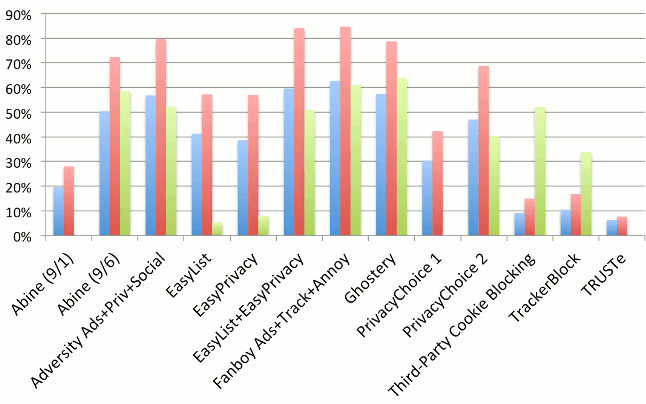
\includegraphics[scale=1.0]{../screenshots/tracking-blocker.png}
\caption{Effektivit�t verschiedener Tracking-Filter}
\label{abb:trackingfilter}
\end{center}
\end{figure}

Aufgrund der Flexibilit�t bei der Einbindung verschiedener Filterlisten empfehle ich \textit{AdBlock Plus}. Mit den Easylist Filterlisten erreichten das Add-on bei dem Test mit die besten Ergebnisse. Die Listen werden st�ndig weiterentwickelt. Es gibt als Zusatz eine spezielle Filterliste f�r deutsche Webseiten.\\

Zus�tzlich zur den Blocklisten\textit{ EasyList+Germany} und \textit{EasyPrivacy} sollte man noch eine Liste abonnieren, die die Social Media Buttons blockiert, z.B. \textit{SocialMediaBlock} von MontzA.\\

\textit{FanBoy} arbeitet seit 2010 mit EasyList zusammen, daher die �hnlich guten Ergebnisse. \textit{Ghostery} schneidet im Test auch gut ab und wird oft empfohlen. Es gibt aber immer wieder Probleme mit Ghostery auf einigen Webseiten, da das Add-on kein Whitelisting kennt. Au�erdem arbeitet es mit einer festen Blockliste, die nicht flexibel erweitert oder kombiniert werden kann. 
\subsection{Adblock f�r Mozilla Firefox}
F�r Mozilla Firefox steht mit \textbf{Adblock Plus}\footnote{ \href{https://addons.mozilla.org/en-US/firefox/addon/adblock-plus/}{https://addons.mozilla.org/en-US/firefox/addon/adblock-plus/}} ein Add-on f�r das listenbasierte Blockieren von Werbung zur Verf�gung. F�r AdBlock Plus gibt es viele Listen zum Blockieren von Werbung (l�nderspezifisch), Tracking-Diensten und der Social Media Like-Buttons. Ein einfacher Klick auf das Install-Symbol der Website startet den Download der Erweiterungen und installiert sie.\\

Nach dem Neustart ist mindestens eine Filterliste zu abonnieren (Bild \ref{abb:adblock1}). Standardm��ig wird f�r deutsche Benutzer die Liste \textit{EasyList Germany + EasyList} vorgeschlagen. \textit{EasyList} ist eine gute Wahl, die man akzeptieren kann.

\begin{figure}[htb]
\begin{center}
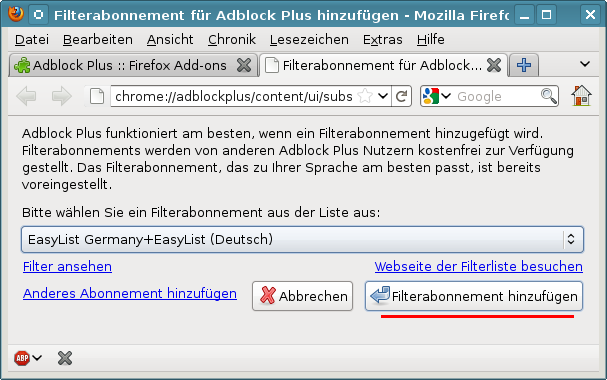
\includegraphics[scale=0.75]{../screenshots/adblock-firststart.png}
\caption{Auswahl einer Liste nach der Installition von Adblock Plus}
\label{abb:adblock1}
\end{center}
\end{figure}

\subsubsection*{Zus�tzliche Filterlisten abonnieren}
Weitere Filterlisten k�nnen im Einstellungen von AdBlock Plus unter dem Men�punkt \textit{Filter Preferences} abonniert werden. Hier ist der Men�punkt \textit{Filter -> Abonnement hinzuf�gen} zu w�hlen. Aus der Liste der angebotenen Filter k�nnen regional passende Listen gew�hlt werden. Folgende Filter-Listen sind als Erg�nzung zur EasyList passend:
\begin{itemize}
 \item \textbf{EasyPrivacy} blockiert meist unsichtbare Tracking-Elemente zum Aussp�hen ihres Verhaltens im Internet mit HTML-Wanzen. Die Liste ist eine sinnvolle Erg�nzung zur EasyList (Germany). Bei der Installation von \textit{EasyPrivacy} kann die zus�tzliche empfohlene EasyList deaktiviert werden, das sie bereits vorhanden ist.
 \item \textbf{SocialMediaBlock} ist eine Liste zum Blockieren der verschiedenen Social Media Tracking Features wie Facebook Like Buttons u.�. Zur Installation kopiert man folgende URL in die Adressleiste von Firefox: \href{abp://subscribe/?location=http://monzta.maltekraus.de/adblock\_social.txt\&title=SocialMediaBlock}{abp://subscribe/?location=http://monzta.maltekraus.de/adblock\_social.txt\&title=SocialMediaBlock}.
\end{itemize}

\subsubsection*{Whitelisting von Websites}
Mit der Version 2.0 hat AdBlock eine Whitelist f�r unaufdringliche Werbung eingef�hrt. Die Filterung wird auf den Webseiten in der Whitelist abgeschaltet, so dass diese Webseiten Werbung einblenden k�nnen. Bisher ist die Whitelist ziemlich leer. Man kann dieses Feature wie in Bild \ref{abb:adblock2} in der �bersicht der Filterlisten abschalten, indem man die Option \textit{Nicht aufdringliche Werbung zulassen} deaktiviert. Alternativ kann man auch das Add-on \textbf{TrueBlock} statt AdBlock verwenden. Es ist 100\% kompatibel mit AdBlock, das Whitelisting ist jedoch standardm��ig deaktiviert. \\

\begin{figure}[htb]
\begin{center}
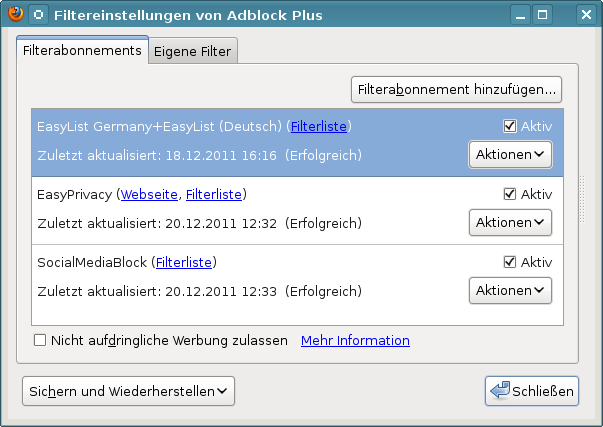
\includegraphics[scale=0.75]{../screenshots/adblock-whitelist.png}
\caption{Whitelisting in AdBlock Plus deaktivieren}
\label{abb:adblock2}
\end{center}
\end{figure}

Statt dessen kann man selbst entscheiden, welchen Webseiten man das Anzeigen von Werbung gestatten m�chte. Mit einem gelegentlichen Klick auf Werbung kann man gute Webseiten bei der Finanzierung unterst�tzen. Wenn Sie eine Webseite im Browser ge�ffnet haben, k�nnen Sie in den Men� von AdBlock die aktuelle Webseite zu einer eigenen Whitelist hinzuf�gen.

\subsubsection*{Vertipper korrigieren}
Die Entwickler von AdBlock sind der Meinung, dass das Korrigieren von Vertippern in der URL ein sinnvolles Feature f�r einen Werbeblocker ist, und haben \textit{URL Fixer} integriert. Die Tippfehlern werden an den Server \textit{urlfixer.org} gesendet und dort gesammelt. Es wird vielen Nutzern nicht gefallen, wenn Daten �ber gerade besuchte Seiten an einen externen Server gesendet werden. Einen Hinweis auf die Daten�bertragung findet man nicht.\\

Man kann dieses (�berfl�ssige) Feature in den Filtereinstellungen von AdBlock auf dem Reiter \textit{Vertipper-Korrekturen} deaktivieren. 

\subsubsection*{Anti-AdBlock}
Anti-AdBlock ist ein Script f�r Webmaster, die den Besucher der Webseite zur Deaktivierung von AdBlock Plus zwingen wollen. Bei aktivem Werbeblocker sieht man beim Besuch einer pr�parierten Webseite nur folgenden Hinweis: 
\begin{center}
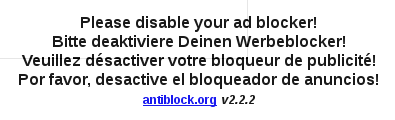
\includegraphics[scale=0.7]{../screenshots/anti-adblock.png}
\end{center}
Wer sich nicht g�ngeln lassen will, kann das Firefox Add-on \textbf{Disable Anti-Adblock}\footnote{ \href{https://addons.mozilla.org/en-US/firefox/addon/disable-anti-adblock/}{https://addons.mozilla.org/en-US/firefox/addon/disable-anti-adblock/}} installieren. Dann kann man die Webseite werbefrei betrachten. 

\section{History Sniffing}
Browser speichern Informationen �ber besuchte Webseiten in einer Surf-History. Eine  empirische Untersuchung der University of California \footnote{ \href{http://cseweb.ucsd.edu/users/lerner/papers/ccs10-jsc.pdf}{http://cseweb.ucsd.edu/users/lerner/papers/ccs10-jsc.pdf}} zeigt, dass ca. 1\% der Top 50.000 Websites versuchen, diese Daten �ber zuvor besuchte Websites auszulesen. Daneben gibt es spezielle Anbieter wie Tealium oder Beencounter, die einem Webmaster in Echtzeit eine Liste der Websites liefern, die ein Surfer zuvor besucht hat. Die dabei �bermittelten Informationen erlauben ein �hnlich detailliertes Interessenprofil zu erstellen, wie das Tracking �ber viele Websites. In der Regel werden die Informationen f�r die Auswahl passender Werbung genutzt.\\

Ein Experiment des Isec Forschungs�labors f�r IT-Sicherheit \footnote{ \href{http://heise.de/-919076}{http://heise.de/-919076}} zeigt, dass diese History-Daten auch zur Deanonymisierung der Surfer genutzt werden k�nnen. Anhand der Browser History wurde ermittelt, welche Gruppen bei Xing der Surfer bisher besucht hat. Da es kaum zwei Nutzer gibt, die zu den gleichen Gruppen geh�ren, konnte mit diesen Daten eine Deanonymiserung erfolgen. Die Realnamen sowie E-Mail Adressen konnten ohne Mithilfe vieler Surfer nur durch den Aufruf der pr�parierten Webseite ermittelt werden.\\

Neben Javascript k�nnen auch CSS-Hacks f�r das Auslesen der Surf-Historie genutzt werden. In der wissenschaftlichen Arbeit \textit{Feasibility and Real-World Implications of Web Browser History Detection} \footnote{ \href{http://www.w2spconf.com/2010/papers/p26.pdf}{http://www.w2spconf.com/2010/papers/p26.pdf}} zeigen Security Experten, wie man die unterschiedliche farbliche Darstellung von bereits besuchten Links auswertet.\\

Die derzeit einzig wirksame Verteidigung besteht in der Deaktivierung der Surf-History. Im Dialog \textit{``Einstellungen``} kann man auf dem Reiter \textit{``Datenschutz''} die Speicherung besuchter Webseiten deaktivieren.

\begin{figure}[htb]
\begin{center}
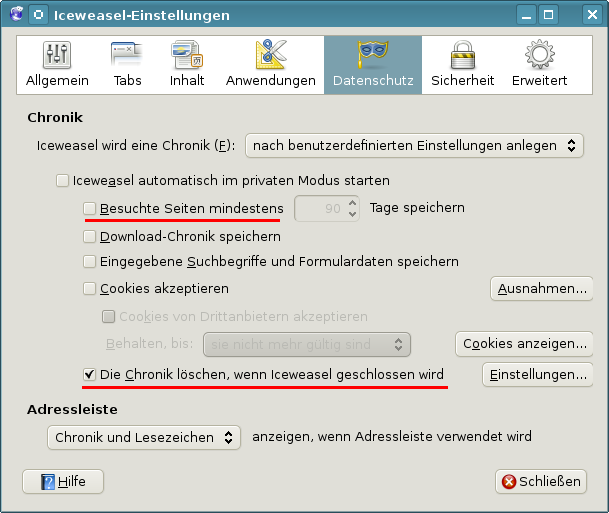
\includegraphics[scale=0.7]{../screenshots/history.png}
\caption{Speichern der Surf-Chronik deaktivieren}
\label{abb:history}
\end{center}
\end{figure}

\section{Browsercache}
Mit jeder aufgerufenen Webseite wird ein ETag gesendet, welches der Browser im Cache speichert. Wird die Webseite erneut aufgerufen, sendet der Browser zuerst das ETag, um zu erfragen, ob die Seite sich ge�ndert hat. Dieses Tag kann eine eindeutige User-ID enthalten. KISSmetrics\footnote{ \href{http://heise.de/-1288914}{http://heise.de/-1288914}} verwendete diese Technik, um gel�schte Tracking-Cookies wieder herzustellen.\\

Ein vollst�ndiges Abschalten des Cache ist nicht empfehlenswert. Man sollte den Cache des Browsers beim Schlie�en automatisch bereinigen. Au�erdem kann man w�hrend des Surfens den Cache usw. mit einer Tastenkombination gelegentlich l�schen.\\

Im Firefox wird der Cache mit weiteren tempor�ren Daten in der \textit{Chronik} zusammengefasst. Die Einstellungen zum L�schen der Chronik findet man unter \textit{Einstellungen} auf dem Reiter \textit{Datenschutz}. Klicken Sie auf den Button \textit{Einstellungen} hinter der Option \textit{Die Chronik l�schen, wenn Firefox geschlossen wird}. In dem sich �ffnenden Dialog kann man detailliert festlegen, welche Daten beim Schlie�en des Browsers gel�scht werden sollen.\\

\begin{figure}[htb]
\begin{center}
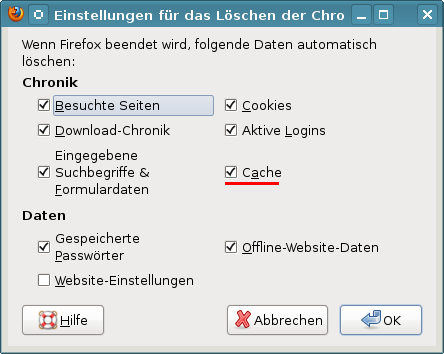
\includegraphics[scale=0.75]{../screenshots/cache_loeschen.png}
\caption{Cache l�schen beim Beenden}
\label{abb:cacheloeschen}
\end{center}
\end{figure}

W�hrend des Surfens kann man die Chronik mit der Tastenkombination STRG-SHIFT-ENTF reinigen oder �ber den Men�punkt \textit{Extra - Neueste Chronik l�schen}.\\

Firefox verwendet einen Cache im Hauptspeicher und einen Disk-Cache auf der Festplatte. Der Cache im Hauptspeicher ist mit 64 MB gro� genug. Den Disk-Cache kann man deaktivieren und damit auch �berfl�ssige Spuren auf dem Rechner vermeiden, die forensisch sichtbar gemacht werden k�nnten. Unter about:config sind daf�r folgende Variablen zu setzen: 
\begin{verbatim}
   browser.cache.disk.enable        false
   browser.cache.disk_cache_ssl     false
   browser.cache.offline.enable     false
\end{verbatim} 

\section{Referer}
Ein Referer liefert die Information, von welcher Seite der Surfer zu der aufgerufenen Webseite gekommen ist, oder bei der Einblendung von Werbung durch Dritte die Information, welche Seite er gerade betrachtet. Es ist ein sehr gut geeignetes Merkmal f�r das Tracking mit Werbung, HTML-Wanzen und Like-Button - die Schleimspur im Web.\\

Die Studie \textit{Privacy leakage vs. Protection measures} \footnote{ \href{http://w2spconf.com/2011/papers/privacyVsProtection.pdf}{http://w2spconf.com/2011/papers/privacyVsProtection.pdf}} zeigt, dass au�erdem viele Web�seiten private Informationen via Referer an Trackingdienste �bertragen. Das folgende Beispiel zeigt den Aufruf eines Werbebanners nach dem Login auf der Webseite http://sports.com
\begin{verbatim}
 GET http://ad.doubleclick.net/adj/....
 Referer: http://submit.sports.com/...?email=name@email.com
 Cookie: id=123456789.....
\end{verbatim}

Mit einer eindeutigen UserID (im Beispiel ein Tracking-Cookie) kann das Surfverhalten �ber viele Webseiten verfolgt werden. Durch zus�tzliche Informationen (im Beispiel eine E-Mail Adresse) werden die gesammelten Datens�tze personalisiert. Im Rahmen der Studie wurde 120 popul�re Webseiten untersucht. 56\% der Webseiten sendeten nach dem Login private Informationen wie E-Mail Adresse, Name oder Wohnort an Trackingdienste.

\subsubsection*{Referer modifizieren f�r Firefox}
Das Add-on \textbf{RefControl} \footnote{ \href{https://addons.mozilla.org/de/firefox/addon/refcontrol/}{https://addons.mozilla.org/de/firefox/addon/refcontrol/}} modifiziert den Referer. Spezifische Einstellungen f�r einzelne Webeiten sind m�glich. Nach der Installation des Plug-Ins sollte im Dialog \textit{Optionen} der Standard-Wert angepasst werden.\\

Die Einstellung \textit{``Blockieren (nur beim Wechsel)``} liefert einen plausiblen Referer,  solange man auf der gleichen Webseite bleibt., entfernt ihn beim Wechsel der Domain. Die Schleimspur wird unterbrochen ohne Funktionen der Website einzuschr�nken.\\

\begin{figure}[htb]
\begin{center}
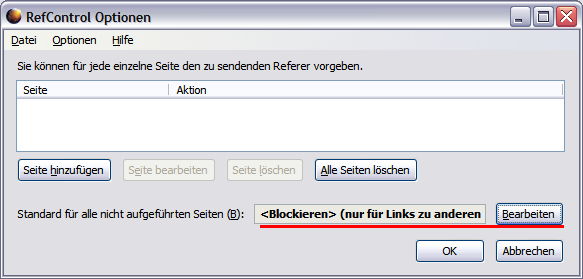
\includegraphics[scale=0.55]{../screenshots/refcontrol1.png}
\caption{Einstellungen von RefControl}
\label{abb:refcontrol}
\end{center}
\end{figure}

Technisch hochentwickelte Datensammler k�nnen den Schutz von RefControl teilweise aushebeln. Google+ und einige Werbenetzwerke �bertragen den Referer zus�tzlich in URL-Parametern. RefControl schadet aber nicht und d�mmere Webmaster tracken auch.

\section{Risiko Plugins}
F�r die Darstellung von Inhalten, die nicht im HTML-Standard definiert sind, kann Firefox Plug-ins nutzen. Popul�r sind Plug-ins f�r die Anzeige von PDF-Dokumenten im Browser oder Flash Videos. Die Nutzung dieser Plug-ins ist jedoch ein Sicherheitsrisiko. Firefox ab Version 14.0 bietet eine einfache M�glichkeit, die Gefahr durch Plug-ins zu reduzieren. Man kann unter der Adresse \textit{about:config} die folgende Variable setzen:
\begin{verbatim}
   plugins.click_to_play  =  true
\end{verbatim} 
Dann werden externe Plug-ins nur aktiviert, wenn der Nutzer es wirklich per Mausklick erlaubt und Drive-By-Download Angriffe sind nicht mehr m�glich.

\subsection{PDF Reader Plugins}
Anwender sind relativ unkritisch gegen�ber PDF-Dokumenten. Was soll beim Anschauen schon passieren? Nur wenige Surfer wissen, dass es mit pr�parierten PDFs m�glich ist, den \textit{ZeuS-Bot} zu installieren und den Rechner zu �bernehmen \footnote{ \href{http://heise.de/-979037}{http://heise.de/-979037}}. 2008 gelang es dem \textit{Ghostnet}, die Rechner�systeme westlicher Regierungen, der US-Regierung und des Dalai Lama mit b�sartigen PDFs zu infizieren \footnote{ \href{http://www.linux-magazin.de/Heft-Abo/Ausgaben/2010/01/Geisterstunde}{http://www.linux-magazin.de/Heft-Abo/Ausgaben/2010/01/Geisterstunde}}. 2012 gelang es dem Trojaner MiniDuke\footnote{ \href{http://heise.de/-1812971}{http://heise.de/-1812971}}, mit b�sartigen PDFs in die Computer von Regierungsorganisationen in Deutschland, Israel, Russland, Gro�britannien, Belgien, Irland, Portugal, Rum�nien, Tschechien und der Ukraine einzudringen. �ber eine von Adobe als \textit{nicht kritisch} eingestufte Sicher�heits�l�cke einer �ber�fl�ssigen PDF-Funktion wurde der Wurm \textit{Win32/Auraax} verteilt \footnote{ \href{http://heise.de/-990544}{http://heise.de/-990544}}...\\

Nach Beobachtung des Sicherheitsdienstleisters Symantec\footnote{ \href{http://heise.de/-981631}{http://heise.de/-981631}} und ScanSafe\footnote{ \href{http://www.scansafe.com/downloads/gtr/2009\_AGTR.pdf}{http://www.scansafe.com/downloads/gtr/2009\_AGTR.pdf}} erfolgen die meisten Angriffe aus dem Web mit b�sartigen PDF-Dokumenten. 2009 wurden f�r ca. 50\% der Angriffe pr�parierten PDF-Dokumente genutzt (mit steigender Tendenz).\\

Schutzma�nahmen: 
\begin{enumerate}
 \item Statt funktions�berladener Monster-Applikationen kann man einfache PDF-Reader nutzen, die sich auf die wesentliche Funktion des Anzeigens von PDF-Dokumenten beschr�nken. Die FSFE stellt auf PDFreaders.org \footnote{ \href{http://www.pdfreaders.org/index.de.html}{http://www.pdfreaders.org/index.de.html}} Open Source Alternativen vor.
\begin{itemize}
 \item F�r Windows werden \textit{Evince} und \textit{Sumatra PDF} empfohlen.
 \item F�r Linux gibt es \textit{Okular} (KDE) und \textit{Evince} (GNOME, XFCE, Unity).
 \item F�r MacOS wird \textit{Vindaloo} empfohlen.
\end{itemize}
\item Wenn die PDF Reader Plugins nicht deinstallierbar sind (keine Adminstrator-Rechte), k�nnen sie im Browser deaktiviert werden. Diese Funktion finden Sie im Addon-Manager unter \textit{Extras -> Add-ons}. PDF-Dokumente sollte man vor dem �ffnen zu speichern und nicht im Kontext des Browsers zu betrachten.
\item Au�erdem sollte man PDF Dokumenten aus unbekannter Quelle ein �hnliches Misstrauen entgegen bringen, wie ausf�hrbaren EXE- oder PAF-Dateien. Man kann einen Online-PDF-Viewer \footnote{ \href{http://view.samurajdata.se/}{http://view.samurajdata.se}} nutzen, um PDF-Dokumente aus dem Internet zu betrachten ohne den eigenen Rechner zu gef�hrden.
\end{enumerate}


\subsection{Java-Applets}
Es gibt eine Vielzahl von sinnvollen Java-Anwendungen. Im Internet spielt Java aber keine Rolle mehr (im Gegensatz zu Javascipt, bitte nicht verwechseln). Trotzdem installiert Oracles Java unter Windows ohne Nachfrage ein Browser-Plugin zum Ausf�hren von Java-Applets, die in Webseiten eingebettet sein k�nnen. Dieses Plug-in ist in erster Linie ein Sicherheitsrisiko und kann zur unbemerkten Installation von Trojanern genutzt werden.\footnote{ \href{http://heise.de/-1485195}{http://heise.de/-1485195}} \footnote{ \href{http://heise.de/-1677249}{http://heise.de/-1677249}} \footnote{ \href{http://heise.de/-1780850}{http://heise.de/-1780850}}\\

Der (Staats-) Trojaner der italienischen Firma \textit{HackingTeam}\footnote{ \href{http://heise.de/-1671203}{http://heise.de/-1671203}} wird beispielsweise mit einer sauber signierten JAR-Datei auf dem Zielsystem installiert. Der Trojaner belauscht Skype, f�ngt Tastatureingaben ab, kann die Webcam zur Raum�berwachung aktivieren und den Standort des Nutzers ermitteln.\\

Als Schutz wird h�ufig die die komplette Deinstallation von Java empfohlen (BSI\footnote{ \href{https://www.bsi.bund.de/ContentBSI/Presse/Pressemitteilungen/Presse2013/Krit\_Schwachstelle\_Java-7-10\_11012013.html}{https://www.bsi.bund.de/ContentBSI/Presse/Pressemitteilungen/Presse2013/Krit\_Schwachstelle\_Java-7-10\_11012013.html}}, DHS\footnote{ \href{http://www.nbcnews.com/technology/technolog/us-warns-java-software-security-concerns-escalate-1B7938755}{http://www.nbcnews.com/technology/technolog/us-warns-java-software-security-concerns-escalate-1B7938755}}, Fefe\footnote{ \href{https://blog.fefe.de/?ts=ae0f1f75}{https://blog.fefe.de/?ts=ae0f1f75}}). Das ist Bullshit und nur sinnvoll, wenn man keine Java-Programme nutzt. Anderenfalls ist die komplette Deinstallation von Java eine unn�tige Einschr�nkung f�r sinnvolle Anwendungen.\\
\begin{itemize}
 \item Aktuelle \textbf{Linux} Distributionen verwenden in der Regel OpenJDK-6/7. Diese Java-JRE installiert KEIN Browser Plug-in. Es besteht also auch keine Gefahr, durch b�sartige Java-Applets aus dem Internet den Rechner zu verseuchen.
 \item Unter \textbf{Windows} bietet die aktuelle Version von Oracles Java die M�glichkeit, die Plug-ins f�r alle Browser unter \textit{Systemsteuerung - Programme - Java} zu deaktivieren (Bild \ref{abb:javadown}).
\begin{figure}[htb]
\begin{center}
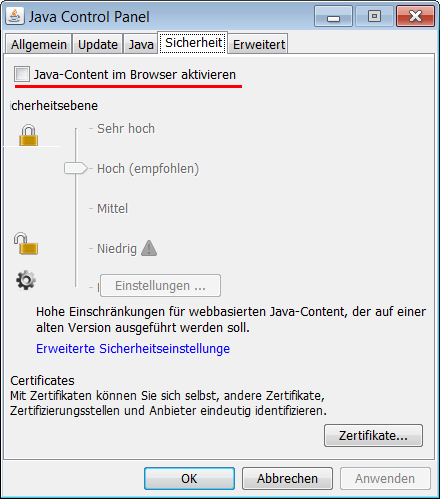
\includegraphics[scale=0.55]{../screenshots/java-ctrl.png}
\caption{Java Plug-in f�r alle Browser deaktivieren}
\label{abb:javadown}
\end{center}
\end{figure}
\end{itemize}

\subsection{Flash und Silverlight}
Auch diese Plugins sind ein Sicherheits- und Privacyrisiko. Sie werden meist f�r die Darstellung von Videos im Web (Youtube) und Panoramadiensten wie Street View (Google) bzw. Street Side (Microsoft) genutzt.\\

Schutzma�nahmen: 
\begin{enumerate}
 \item Das Add-on \textbf{NoScript} kann diese Inhalte blockieren. Es wird ein Platzhalter angezeigt. Bei Bedarf kann man das Video mit einem Mausklick anschauen.
\item Web Videos k�nnen mit Hilfe von Download Sites wie KeepVid \footnote{ \href{http://keepvid.com}{http://keepvid.com}} oder ShareTube \footnote{ \href{http://www.share-tube.de/flvdownload.php}{http://www.share-tube.de/flvdownload.php}} gespeichert und mit einem Mediaplayer abgespielt werden.
\item Die Firefox Add-ons \textbf{UnPlug} \footnote{ \href{https://addons.mozilla.org/en-US/firefox/addon/unplug/}{https://addons.mozilla.org/en-US/firefox/addon/unplug}} oder \textbf{DownloadHelper} \footnote{ \href{https://addons.mozilla.org/de/firefox/addon/video-downloadhelper/}{https://addons.mozilla.org/de/firefox/addon/video-downloadhelper}} k�nnen Videos von vielen Websites herunter laden und dabei in ein gebr�uchlicheres Format f�r Mediaplayer konvertieren.
\end{enumerate}
Wer noch keinen passenden Mediaplayer installiert hat, kann den VideoLAN Player nutzen (VLC-Player), der f�r alle Betriebssysteme zur Verf�gung steht.

\subsection{Weitere Anwendungen}
Neben PDF-Dokumenten k�nnen auch alle anderen Dokument-Typen f�r Drive-by-Donwload Angriffe verwendet werden. Um diese zu unterbinden, sollte man externe Anwendungen f�r Dateien nur nach Best�tigung durch den Anwender �ffnen lassen. Anderenfalls k�nnen Bugs in diesen Anwendungen automatisiert genutzt werden.\\

\begin{figure}[htb]
\begin{center}
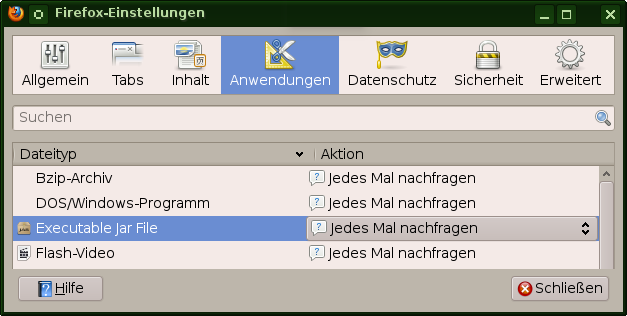
\includegraphics[scale=0.65]{../screenshots/ff-anwendungen.png}
\caption{Externe Anwendungen nur auf Nachfrage �ffnen}
\label{abb:ffhelper}
\end{center}
\end{figure}

Auf dem Reiter \textit{Anwendungen} im Dialog \textit{Einstellungen} k�nnen die Helper-Applications wie im Bild \ref{abb:ffhelper} f�r jeden Dateityp auf \textit{``Jedes Mal nachfragen``} gesetzt werden. Diese Einstellungen sind nat�rlich nur sinnvoll, wenn der Surfer kritisch hinterfragt, ob die Aktion wirklich dem entspricht, was er erwartet. Wer unkritisch bei jeder Nachfrage auf \textit{�ffnen} klickt, muss sich nicht wundern, wenn sein Computer infiziert wird.
\section{HTTPS nutzen}
Viele Websites bieten HTTPS-Verschl�sselung an. Diese sichere Daten�bertragung wird h�ufig nicht genutzt. Mit wenig Konfigurationsaufwand l�sst sich die Nutzung von HTTPS f�r eine definierte Liste von Websites erzwingen.

\subsubsection*{NoScript Enforce HTTPS}
NoScript Enforce HTTPS ist einfach konfigurierbar, kann aber nur \textit{http://} durch \textit{https://} f�r eine Liste von Websites ersetzen. Die Liste muss man per Hand erstellen. Im Dialog \textit{Einstellungen} findet man auf dem Reiter \textit{Erweitert} unter \textit{HTTPS} eine editierbare Liste von Websites.\\

\begin{figure}[htb]
\begin{center}
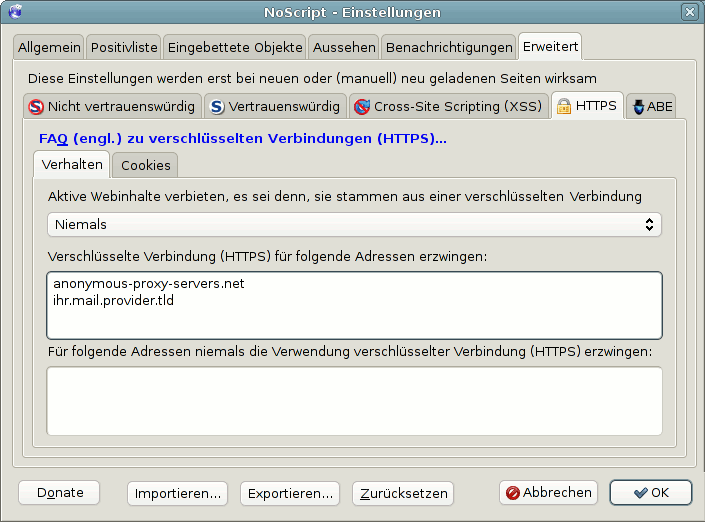
\includegraphics[scale=0.7]{../screenshots/noscript_STS.png}
\caption{Einstellungen f�r NoScript STS}
\label{abb:noscriptsts}
\end{center}
\end{figure}

Standardm��ig ist die Liste leer. Wer das Webinterface eines E-Mail Providers nutzt, sollte die Domain hier eintragen. Au�erdem sollte man die Webseite der Bank eintragen, wenn man Online-Banking nutzt.

\subsubsection*{HTTPS-Everywhere}
Das Firefox Add-on HTTPS-Everywhere\footnote{ \href{https://www.eff.org/https-everywhere}{https://www.eff.org/https-everywhere}} der EFF.org kann auch komplexe Umschreibungen der URLs realisieren, wie es beispw. f�r Wikipedia notwendig ist. Das Add-on bringt aber bereits �ber 2500 Regeln f�r h�ufig genutzte Webseiten mit. Die Konfiguration eigener Regeln ist aufwendiger als bei NoScript und erfolgt �ber XML-Dateien.\\

Bei HTTPS-Everywhere sind Regeln standardm��ig deaktiviert, wenn der Server ein SSL-Zertifikat von CAcert.org nutzt (z.B www.ccc.de) Wenn Sie das Root-Zertifikat von CAcert.org im Browser importiert haben, dann k�nnen Sie diese Regeln in den Einstellungen von HTTPS-Everywhere mit Klick auf das Kreuz aktivieren (Bild \ref{abb:httpseverywherecacert}).

\begin{figure}[htb]
\begin{center}
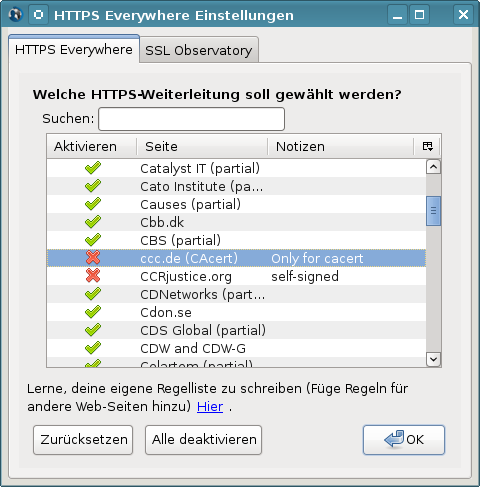
\includegraphics[scale=0.75]{../screenshots/httpseverywhere.png}
\caption{Einstellungen f�r Https-Everywhere}
\label{abb:httpseverywherecacert}
\end{center}
\end{figure}

\subsubsection*{HTTPS-Finder}
Das Add-on HTTPS-Finder\footnote{ \href{https://addons.mozilla.org/de/firefox/addon/https-finder/}{https://addons.mozilla.org/de/firefox/addon/https-finder/}} kann erkennen, ob eine Webseite auch via HTTPS erreichbar ist und erzwingt dann die Nutzung von HTTPS. Es k�nnen automatisch Regeln f�r HTTPS-Everywhere erstellt und aktiviert werden. Das Add-on ist eine gute Erg�nzung f�r HTTPS-Everywhere und erspart das komplexe Erstellen der XML-Dateien von Hand.\\


\section{Vertrauensw�rdigkeit von HTTPS}
IT-Sicherheitsforscher der EFF kommen in einer wissenschaftlichen Arbeit\footnote{ \href{https://eff.org/deeplinks/2010/03/researchers-reveal-likelihood-governments-fake-ssl}{https://eff.org/deeplinks/2010/03/researchers-reveal-likelihood-governments-fake-ssl}} zu dem Schluss, dass Geheim�dienste mit g�ltigen SSL-Zertifikaten schwer erkennbare man-in-the-middle Angriffe durchf�hren k�nnen. Diese Angriffe k�nnen routinem��ig ausgef�hrt werden, schreibt die EFF:
\begin{quote}
 \textit{Certificate-based attacks are a concern all over the world, including in the U.S., since governments everywhere are eagerly adopting spying technology to eavesdrop on the public. Vendors of this technology seem to suggest the attacks can be done routinely.}
\end{quote} 
\begin{enumerate}
 \item Ein erster Angriff dieser Art gegen iranische Internet Nutzer wurde im August 2011 nachgewiesen. Er betraf neben Google die Webdienste mehrerer Geheimdienste (MI6, CIA, Mossad) und au�erdem www.torproject.org. Bei diesem Angriff wurde keine Zertifikate einer standardm��ig vertrauensw�rdigen Certification Authority genutzt, sondern die niederl�ndische Certification Authority DigiNotar wurde gehackt, um g�ltige Zertifikate zu erlangen. Insgesamt wurden 531 SSL-Zertifikate kompromittiert.\footnote{ \href{https://threatpost.com/en\_us/blogs/final-report-diginotar-hack-shows-total-compromise-ca-servers-103112}{https://threatpost.com/en\_us/blogs/final-report-diginotar-hack-shows-total-compromise-ca-servers-103112}}

 \item Neben DigiNotar wurden 2011 die Certification Authorities Comodo, InstantSSL und zwei weitere Sub-Registrare von Comodo erfolgreich angegriffen \footnote{ \href{http://heise.de/-1213999}{http://heise.de/-1213999}}. Die Angreifer konnten sich unbefugt g�ltige Zertifikate f�r die Webseiten von Google, Yahoo, Mozilla und Skype erstellen. Nach Beobachtung des SSL-Observatory der EFF wurden bei den Angriffen mindesten 248 Zertifikate erfolgreich kompromittiert. Auch in diesen F�llen soll der Angriff vom Iran ausgegangen sein.
\end{enumerate}


Die Software f�r einen man-in-the-middle Angriff mit den gef�lschten Zertifikaten gibt es auch als Open Source, z.B. den mitm-proxy\footnote{ \href{http://crypto.stanford.edu/ssl-mitm/}{http://crypto.stanford.edu/ssl-mitm/}} der Stanford University oder dsniff \footnote{ \href{http://www.monkey.org/~dugsong/dsniff/}{http://www.monkey.org/~dugsong/dsniff/}}. Auf der ISS World (Messe f�r �bewachungstechnik) werden fertige Appliances angeboten, gegen Aufpreis auch mit g�ltigem CA-Zertifikat.\\

Wer Kosten (f�r den Aufpreis) oder M�hen (f�r das Hacken einer CA) scheut, kann sich so einfach als Unberechtigter ein g�ltiges SSL-Zertifikat f�r einen Mail- oder Web-Server ausstellen zu lassen \footnote{ \href{https://bugzilla.mozilla.org/show\_bug.cgi?id=556468}{https://bugzilla.mozilla.org/show\_bug.cgi?id=556468}}. Man muss nur einen der zul�ssigen E-Mail Accounts f�r SSL-Admins registrieren und kann ein g�ltiges Fake-Zertifikat erstellen. Par ordre du mufti werden \textit{webmaster\@domain.tld, postmaster\@domain.tld, ssladmin\@domain.tld, ssladministrator\@domain.tld} u.a.m. von den Certification Authorities akzeptiert. Nicht immer sind diese Adressen reserviert und gesch�tzt.

\subsubsection*{Verbesserung der Vertrauensw�rdigkeit von HTTPS}
Es gibt einige M�glichkeiten, die Vertrauensw�rdigkeit der HTTPS-Verschl�sselung zu verbessern und Angriffe mit falschen Zertifikaten zu erschweren.
\begin{itemize}
 \item \textbf{Zertifikate speichern:} Beim ersten Besuch der Webseite wird das SSL-Zertifikat gespeichert. Bei sp�teren Besuchen wird das aktuelle Zertifikat mit dem gespeicherten Zertifikat verglichen. Bei seltsamen Abweichungen wird eine Warnung angezeigt, die der Surfer allerdings bewerten muss. (Firefox Add-ons: Certificate Patrol, JonDoFox)
\item \textbf{Vergleich mit Anderen:} Beim Besuch einer HTTPS-verschl�sselten Webseite wird das Zertifikat mit den Ergebnissen an anderen Punkten der Welt verglichen. Wenn alle Teilnehmer des Netzes das gleiche Zertifikat sehen, ist es wahrscheinlich Ok. Dieser Vergleich kann mit einer zeitlich begrenzten Speicherung kombiniert werden.\\
(Firefox Add-ons:  HTTPS-Everywhere, Perspectives, Convergence.io)\\Obwohl die Idee auf den ersten Blick einleuchtend ist, gibt es einige Probleme bei gro�en Serverfarmen wie Google, Facebook, Amazon, PayPal... Diese Serverfarmen verwenden nicht immer ein einheitliches Zertifikat. Das f�hrt zu Verwirrung bei einem externen Beobachter und zu inkonsistenten Ergebnissen der Notary Server. 

 \item \textbf{Certificate Pinning:} Nur der Betreiber einer Webseite kann wirklich wissen, welche Zertifikate g�ltig sind. Diese Information muss verteilt und ausgewertet werden. Das w�re ein besserer Weg, als der Vergleich mit externen Beobachtern.\\
�ber einen unabh�ngigen Weg wird festgelegt, welche Zertifikate f�r die HTTPS-Verschl�sselung einer Webseite genutzt werden d�rfen. Nur diese Zertifikate werden vom Browser akzeptiert. Google hat die Fingerprints der Zertifikate seiner Webseiten fest im Browser Chrome codiert. Dieses Verfahren skaliert aber nicht. M�glich w�re auch die Nutzung von DNSSEC mittels Sovereign Keys. Brauchbare Ideen zum Certificate Pinning sind noch in der Entwicklung.
\end{itemize}

\subsection{Firefox Add-ons}
Ein paar kleine Erweiterungen f�r Firefox, welche die Vertrauensw�rdigkeit der Zertifikate bei der Nutzung von HTTPS-ver�schl�sselten Verbindungen deutlich erh�hen k�nnen. 

\subsubsection*{HTTPSEverywhere}
HTTPS-Everywhere\footnote{ \href{https://www.eff.org/https-everywhere}{https://www.eff.org/https-everywhere}} kann das SSL-Obervatory der EFF.org nutzen. Wenn man diese Funktion in den Einstellungen des Add-on aktiviert (Bild \ref{abb:sslobservatory}), werden die SSL-Zertifikate der besuchten Webseiten an das SSL-Observatory gesendet. Ist das Zertifikat nicht ok, wird man ab Version 3.0 gewarnt. Es wird eine Datenbasis von weltweit verteilten Nutzern aufgebaut.\\

Hinweis: Aufgrund eines Bug im Proxy-Handling sollte das SSL-Observatory nicht mit dem Anonymisierungsdienst JonDonym genutzt werden. Die Proxy-Einstellungen werden von HTTPSEverywhere ignoriert. In Kombination mit TorButton (TorBrowser) soll dieser Bug nicht auftreten.

\begin{figure}[p]
\begin{center}
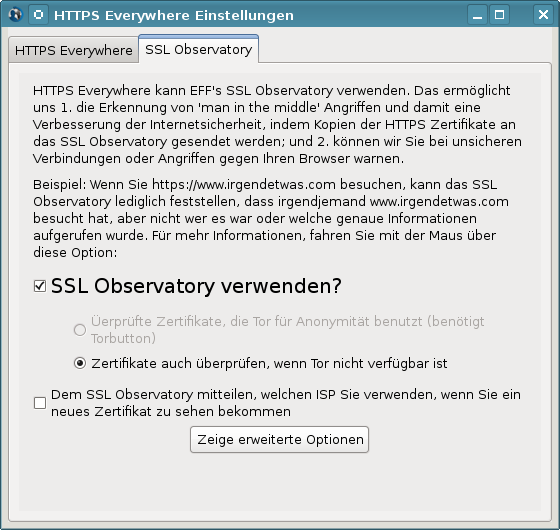
\includegraphics[scale=0.75]{../screenshots/ssl-observatory.png}
\caption{SSL-Observatory aktivieren in HTTPS-Everywhere}
\label{abb:sslobservatory}
\end{center}
\end{figure}

\subsubsection*{Certificates Patrol}
Certificates Patrol \footnote{ \href{https://addons.mozilla.org/de/firefox/addon/certificate-patrol/}{https://addons.mozilla.org/de/firefox/addon/certificate-patrol/}} speichert Informationen zu den Zertifikaten einer Website in einer internen Datenbank. Beim Erstbesuch wird mit einem Informationsbalken am oberen Seitenrand auf ein neues Zertifikat hingewiesen. Man kann es bei Bedarf �berpr�fen. Am einfachsten kann man ein SSL-Zertifikat pr�fen, wenn die Fingerprints vom Webmaster ver�ffentlicht wurden.\\

\begin{figure}[p]
\begin{center}
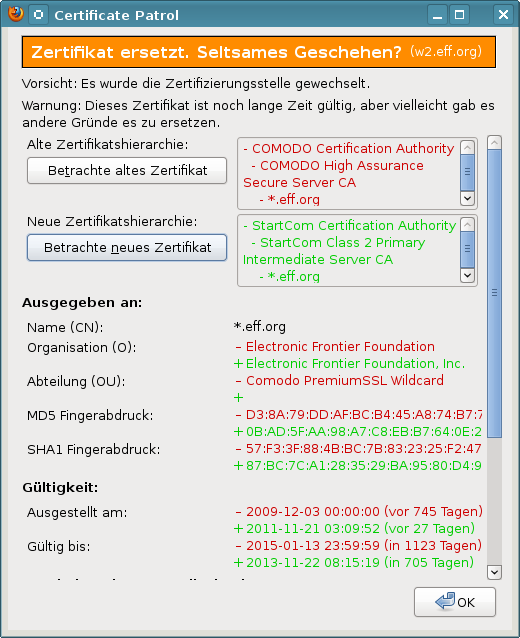
\includegraphics[scale=0.75]{../screenshots/patrol.png}
\caption{Warnung bei setsamen Wechsel des SSL-Zertifikat}
\label{abb:certificatespatrol}
\end{center}
\end{figure}

Hat sich das Zertifikat bei sp�teren Besuchen der Website ge�ndert, zeigt das Add-on Informationen oder Warnungen zum Zertifikatswechsel wie im Bild \ref{abb:certificatespatrol} gezeigt. Der Gefahrenwert wird dabei anhand einer Heuristik ermittelt. Im Beispiel wurde �berraschend ein neues Zertifikat f�r die Webseite der EFF gefunden, obwohl das alte Zertifikat noch lange g�ltig gewesen w�re. Au�erdem wurde die CA gewechselt. Der Nutzer muss bei Warnungen das neue Zertifikat best�tigen, da es ein Hinweis auf einen Angriff sein. Wie kann man pr�fen, ob der Zertifikatswechsel ok ist?
\begin{enumerate}
 \item H�ufig ver�ffentlicht der Webmaster der Seite eine Information zum Zertifikatswechsel im Blog mit den Informationen zum neuen Zertifikat.
 \item Bei Banken u.�. Diensten kann man telefonisch nachfragen, ob das SSL-Zertifikat ge�ndert wurde.
 \item Man kann pr�fen, welches Zertifikat andere Teilnehmer im Netz sehen, beispielsweise mit dem Add-on \textit{Perspectives} (siehe unten). Das Projekt bietet auch eine Demo-Webseite \footnote{ \href{http://data.networknotary.org/notary\_web/notary\_query}{http://data.networknotary.org/notary\_web/notary\_query}}, wo man die Informationen der Notary Server abfragen kann. 
\end{enumerate}

\subsubsection*{Perspectives}
Perspectives\footnote{ \href{https://addons.mozilla.org/en-US/firefox/addon/perspectives/}{https://addons.mozilla.org/en-US/firefox/addon/perspectives/}} vergleicht SSL-Zertifikate mit den bei Notary Servern bekannten Zertifikaten. Wenn alle Notary-Server das gleiche Zertifikat �ber einen l�ngeren Zeitraum sehen, ist es wahrscheinlich g�ltig. Leider gibt es noch nicht viele, international verteilte Notary Server. Alle standardm��ig im Add-on enthaltenen Server werden vom MIT bereit gestellt.\\

Aufgrund der nicht immer eindeutigen Resultate und der Performance der Notary Server ist Perspectives nicht unbedingt f�r eine st�ndige Validierung aller SSL-Zertifikate geeignet. Der Server awxcnx.de ist im Moment nur bei der H�lfte der Notary Server bekannt. Das f�hrt zu einem Fehler bei Perspectives, obwohl eigentlich alles Ok ist.\\

Ich empfehle daher die Abfrage der Notarys bei Bedarf (wenn man ein Zertifikat genauer pr�fen m�chte). Daf�r sind die Einstellungen in den Preferences wie im Bild \ref{abb:perspectives} zu setzen.\\

\begin{figure}[htb]
\begin{center}
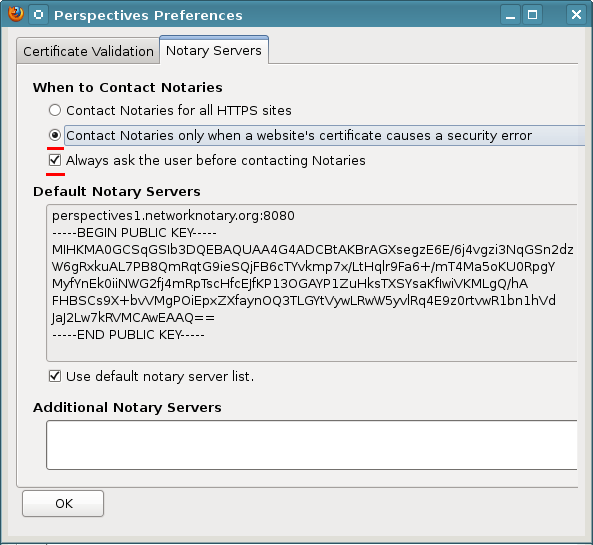
\includegraphics[scale=0.75]{../screenshots/perspectives.png}
\caption{Perspectives Konfiguration}
\label{abb:perspectives}
\end{center}
\end{figure}

Zuk�nftig kann man mit einem Klick der rechten Maustatste auf das Perspectives-Symbol in der Statusleiste einen Check des Zertifikates der Webseite erzwingen und sich die Notary Results anzeigen lassen.\\

\subsubsection*{Convergence.io}
Convergence (Beta): W�hrend Certificate Patrol und Perspectives auf dem alten Zertifikats�system aufsetzen und es etwas verbessern, vollzieht Convergence.io einen radikalen Bruch. Das Add-on ersetzt die Validierung der Zertifikate im Firefox vollst�ndig durch ein eigenes System. Dabei werden �hnlich wie bei Perspectives die Beobachtungen von Notary Server genutzt und mit dem aktuellen Zertifikat verglichen.\\ 

Ich habe (noch) keine Erfahrungen mit Convergence.io gesammelt.

\section{HTTPS Tracking}
Beim Aufbau einer verschl�sselten HTTPS-Verbindung wird eine sogenannte Session initialisert. Die kryptografischen Details sollen an dieser Stelle nicht erl�utert werden.\\

Es ist m�glich, diese HTTPS-Session f�r das Tracking zu nutzen und f�r bis zu 48h immer wieder zu erneuern. Dieses Tracking-Verfahren ist so gut wie nicht nachweisbar, da es voll�st�ndig durch den Webserver realisiert wird und keine Spuren im Browser hinterl�sst. Man kann davon ausgehen, dass dieses Tracking als Erg�nzung zu (Ever-) Cookies genutzt wird. Der Tracking-Service Woopa verwendet seit 2008 HTTPS Session Tracking.\\

F�r HTTPS Session Tracking gibt es zwei M�glichkeiten:
\begin{description}
 \item[Tracking via Session Resumption] ist im RFC 5077 beschrieben.

 Gegen Tracking via Session Resumption kann man sich sch�tzen, indem man im Firefox unter \textit{about:config} die folgende Variable auf FALSE setzt:  
\begin{verbatim}
  security.enable_tls_session_tickets    false  
\end{verbatim} 
Das f�hrt zu geringen Einbu�en der Performance, da f�r jede Seite eine neue SSL-Session ausgehandelt werden muss. Um die Performance-Einbu�en etwas zu kompensieren, kann man \textit{SSL False Start} aktivieren. Dabei werden verschl�sselte Daten bereits gesendet, wenn die Verifizierung der SSL-Session noch nicht abgeschlossen ist. Ein Sicherheitsrisiko besteht dabei nicht. Sollte die Verifizierung der SSL-Session fehlschlagen, werden die bereits empfangenen Daten verworfen.
\begin{verbatim}
  security.ssl.enable_false_start    true  
\end{verbatim}

 \item[Tracking via SSL-Session-ID] wird ebenfalls von allen Webserven unterst�tzt. Auch Webshops k�nnen die Session-ID f�r das Tracking verwenden, z.B. die \textit{xtcModified eCommerce Shopsoftware}\footnote{ \href{http://www.modified-shop.org/wiki/SESSION\_CHECK\_SSL\_SESSION\_ID}{http://www.modified-shop.org/wiki/SESSION\_CHECK\_SSL\_SESSION\_ID}}.\\

Gegen das Tracking via Session-ID sch�tzen nur das TorBrowserBundle und der JonDoBrowser (Beta). Man kann sich nicht durch Konfigurationseinstellungen oder Add-ons sch�tzen, da der Source-Code des Browser daf�r modifiziert werden muss.
 \end{description}




\section{Starke Passw�rter nutzen}
Jeder kennt das Problem mit den Passw�rtern. Es sollen starke Passw�rter sein, sie sollen f�r jede Site unterschiedlich sein und au�erdem soll man sich das alles auch noch merken und auf keinen Fall auf einen Zettel unter der Tastatur ``speichern''. 

\begin{itemize}

\item Was ist ein starkes Passwort? Diese Frage muss man unter Beachtung des aktuellen Stand der Technik beantworten. W�rterbuchangriffe sind ein alter Hut. Das Passwort darf kein Wort aus dem Duden sein, das ist einfach zu knacken. F�r zuf�llige Kombinationen aus Buchstaben, Zahlen und Sonderzeichen kann man Cloud Computing f�r Brute Force Angriffe nutzen. Dabei werden alle m�glichen Kombinationen durchprobiert. Ein 6-stelliges Passwort zu knacken, kostet 0,16 Euro. Eine 8-stellige Kombination hat man mit 400 Euro wahrscheinlich und mit 850 Euro sicher geknackt. Man sollte mindestens 10...12 Zeichen verwenden. (Stand: 2011)

 \item Warum sollte man nicht das gleiche Passwort f�r viele Logins verwenden? Diese Frage beantwortet der Hack von Anonymous gegen HBGary. Den Aktivisten von Anonymous gelang es, Zugang zur User-Datenbank des Content Management Systems der Website zu erlangen. Die Passw�rter konnten geknackt werden. Die Passw�rter wurden vom F�hrungspersonal f�r weiterer Dienste genutzt: E-Mail, Twitter und Linked-In. Die ver�ffentlichten 60.000 E-Mails waren sehr peinlich f�r HBGary \footnote{ 
 \href{http://www.heise.de/ct/artikel/Ausgelacht-1195082.html}{http://www.heise.de/ct/artikel/Ausgelacht-1195082.html}}.
\end{itemize}


Das Add-on \textbf{PwdHash}\footnote{ \href{https://addons.mozilla.org/de/firefox/addon/pwdhash/}{https://addons.mozilla.org/de/firefox/addon/pwdhash/}} vereinfacht den Umgang mit Passw�rtern. Wenn man vor der Eingabe des Passwortes die Taste F2 dr�ckt oder mit einem doppelten @@ beginnt,  wird es in einen einen Hash aus dem Master Passwort und der Domain umgerechnet. Das Ergebnis der Berechnung ist eine 10-stellige zuf�llige Kombination von Buchstaben und Zahlen und wird als Passwort gesendet. Damit ist es m�glich, ein merkbares Master-Passwort f�r alle Sites zu nutzen, bei denen PwdHash funktioniert. Wichtig ist, dass die Domains der Webseiten f�r die �nderung und Eingabe der Passw�rter identisch sind.\\

PwdHash sch�tzt auch vor Phishing-Angriffen. Da die Seite des Phishers von einer anderen Domain geliefert wird, als die originale Website, wird ein falscher Hash generiert, der f�r den Angreifer wertlos ist.\\

Sollte man unterwegs auf einem Rechner das Add-on nicht installiert haben, ist das Login-Passwort nat�rlich nicht zu erraten. Auf der Website des Projektes \footnote{ \href{https://www.pwdhash.com}{https://www.pwdhash.com}} steht der Algorithmus auch als Javascript Applet zur Verf�gung. Man kann sein Master Passwort und die Domain eingeben und erh�lt das generierte Login Passwort. Das kann  man mit Copy \& Paste in das Passwort Eingabefeld �bernehmen.

\subsubsection*{Passwortspeicher}
Passwortspeicher sind kleine Tools, die Username/Passwort Kombinationen und weitere Informationen zu verschiedenen Accounts in einer verschl�sselten Datenbank verwalten. Es gibt mehrere Gr�nde, die f�r die Verwendung eines Passwortspeichers sprechen:
\begin{itemize}
 \item Viele Programme wie Pidgin oder Jitsi speichern Passw�rter unverschl�sselt auf der Festplatte, wenn man die Option zur Speicherung aktiviert (nicht empfohlen!). Andere Programme bieten keinen M�glichkeit zur Speicherung von Passw�rtern, fordern aber die Nutzung einer m�glichst langen, sicheren Passphrase (z.B LUKS oder Truecrypt).
 \item Bei vielen Accounts muss man sich neben Unsername und Passwort weitere Informationen merken wie z.B. die Antwort auf eine Security Frage oder PINs bei Bezahldienstleistern.
 \item In der Regel enthalten Passwortspeicher eine Passwortgenerator, der wirklich zuf�llige und starke Passw�rter generieren kann.
 \item Das Backup wird deutlich vereinfacht. Man muss nur die verschl�sselte Datenbank auf ein externes Backupmedium kopieren.
\end{itemize}

Mir gef�llt \textit{Keypass}\footnote{ \href{http://keypass.en.softonic.com/}{http://keypass.en.softonic.com}} (Windows) bzw. \textit{KeepassX} (Linux) sehr gut. Die Bedienung ist �ber�sichtlich. Man kann Eintr�ge gruppieren, komplizierte Passworte k�nnen �ber die Zwischen�ablage in die Eingabefelder kopiert werden und m�ssen nicht (fehlerhaft) abgetippt werden.
Um krypto�analytische Angriffe zu erschweren, kann man die Datenbank mehrere 10.000x mit AES256 verschl�sseln.\\

\begin{figure}[htb]
\begin{center}
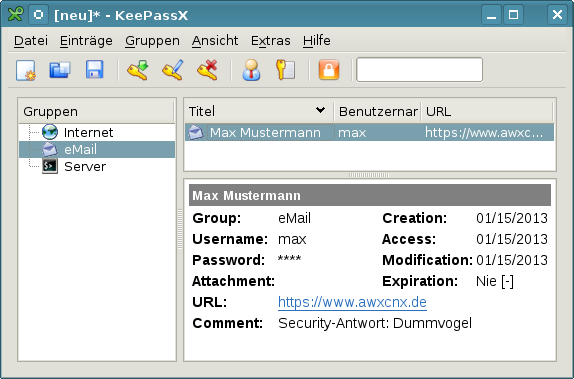
\includegraphics[scale=0.75]{../screenshots/keypass.png}
\caption{KeepassX Hauptfenster}
\label{abb:keypass}
\end{center}
\end{figure}

Einige Passwortspeicher werben mit der M�glichkeit, die Datenbank zwischen verschiedenen Rechnern und Smartphones zu synchronisieren. Dabei wird die Datenbank \textit{in der Cloud} gespeichert. Das ist f�r mich ein Graus, vor allem, weil der geheimdienstliche Zugriff auf Daten \textit{in der Cloud} immer mehr vereinfacht wird.\footnote{ \href{https://www.awxcnx.de/gedanken-bestandsdaten.htm}{https://www.awxcnx.de/gedanken-bestandsdaten.htm}}
\section{HTTP-Header filtern}
Neben der Verwendung von Cookies wird auch der Inhalt des HTTP-Header f�r die Gewinnung von Informationen �ber den Surfer genutzt. Das Projekt \textit{Panopticlick} \footnote{ \href{http://panopticlick.eff.org/}{http://panopticlick.eff.org}} der EFF.org zeigt, dass anhand des Fingerprint des HTTP-Headers 80\% der Surfer eindeutig erkennbar sind. Eine Verkn�pfung dieser Information �ber mehrere Websites hinweg kann eine Verfolgung von Nutzern erm�glichen. Kombiniert man diese Verfolgung mit Daten von Sozialen Netzen (Facebook, Xing), ist eine vollst�ndige Deanonymiserung m�glich.
\begin{itemize}
\item Beispiel \textbf{User-Agent}: Die meisten Browser senden Informationen �ber den verwendeten Browser und das Betriebssystem. Ein Beispiel zeigt, wie detailliert der Browser Auskunft gibt:
\begin{verbatim}
Mozilla/5.0 (Macintosh; U; PPC Mac OS X; de-DE) AppleWebKit/419.3 
(KHTML, like Gecko) Safari/419.3
\end{verbatim}
Beim US-Reiseportal Orbitz werden Surfern mit MacOS (am User-Agent erkennbar) die Hotelzimmer 20-30 Dollar teuerer angeboten, als anderen Kundern\footnote{ \href{http://heise.de/-1626368}{http://heise.de/-1626368}}. Au�erdem k�nnen anhand der Informationen gezielt L�cken in der verwendeten Software ausgenutzt werden.\\


\item Erg�nzende Informationen wie zum Beispiel die bevorzugte \textbf{Sprache}, installierte \textbf{Schrift�arten} und \textbf{Gr��e des Browserfensters} k�nnen einen individuellen Fingerprint des Browsers ergeben. Viele Werte k�nnen per Javascript ausgelesen werden Bei der Google-Suche und beim Trackingdienst Multicounter\footnote{ \href{http://www.multicounter.de/features.html}{http://www.multicounter.de/features.html}} wird die innere Gr��e des Browser�fensters ausgelesen. Die Firma bluecave\footnote{ \href{http://www.bluecava.com/}{http://www.bluecava.com}} nutzt z.B. im Trackingscript \textit{BCAL5.js} u.a. Informationen �ber installierte Schriftarten.\\

Deshalb sollte man Javascript nur f�r vertrauensw�rdige Webseiten erlauben und das Auslesen der Werte behindern (soweit m�glich).
\end{itemize} 


\subsubsection*{Installierte Schriftarten verstecken f�r Firefox}
Um die installierten Schriftarten zu verstecken, deaktiviert man in den Einstellungen die Option \textit{Webseiten das verwenden von eigenen Schriften erlauben}. Man findet die Option in den Firefox \textit{Einstellungen} auf dem Reiter \textit{Inhalt}. Klicken Sie auf den Button \textit{Erweitert}, um im folgenden Dialog Bild \ref{abb:schriftarten} die Option zu deaktivieren.\\

\begin{figure}[htb]
\begin{center}
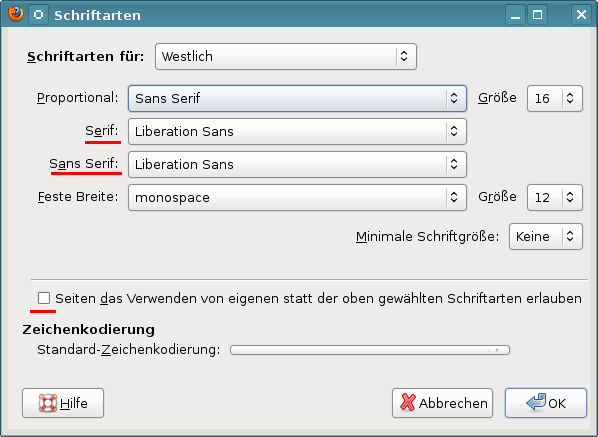
\includegraphics[scale=0.75]{../screenshots/schriftarten.png}
\caption{Schriftarten}
\label{abb:schriftarten}
\end{center}
\end{figure}

Damit kann man nur ''3'' Schriftarten auslesen. Der Browser verwendet aber auch nur die drei Standardschriften zur Darstellung der Webseiten. Damit sehen nicht alle Webseiten exakt so aus, wie es sich der Designer w�nscht. Um die Lesbarkeit zu verbessern, sollten man au�erdem gut lesbare Standardschriften verwenden. Unter Windows eignet sich \textit{Arial}, unter Linux nutzt man am besten \textit{Liberation Sans} (siehe Screenshot).


\subsubsection*{User-Agent modifizieren f�r Firefox}
Es ist nicht so einfach, den User Agent plausibel zu faken. Um durch unsachgem��e �nderung keine eindeutige Kennung zu generieren, sollte man nachdenken, bevor man etwas �ndert.\\

Man kann f�r einen Firefox nur eine andere Firefox-Kennung verwenden. Da die Browser durch individuelle Header erkennbar sind, ist eine Tarnung mit dem User-Agent eines anderen Browsers leicht als Fake zu identifizieren und man ist eindeutig identifizierbar. Einige Firefox Versionen unterscheiden sich nicht nur im User-Agent, sondern auch sehr subtil in einigen anderen HTTP-Headern. Man beachte das Leerzeichen nach dem Komma bei FF 10.0:\\
\begin{verbatim}
 ACCEPT-ENCODING "gzip,deflate"      (Firefox 3.6.x)
 ACCEPT-ENCODING "gzip, deflate"     (Firefox 10.0.x)
\end{verbatim} 

Deshalb muss man auch eine �hnliche Firefox-Version f�r den Fake nutzen, die sich in den �brigen HTTP-Headern nicht unterscheidet.Die meisten Firefox-User nutzen Windows als Betriebssystem. Daher sollte man einen Fake von Firefox f�r Windows nutzen, um in einer gr��eren Anonymt�tsgruppe abzutauchen. F�r Windows Nutzer empfehle ich keine Fakes, da man durch kleine Fehler nur eindeutiger identifizierbar wird.\\

Um die User-Agent Kennung zu �ndern, gibt man in der Adresszeile "about:config" ein und setzt die angebenen Variablen auf die Werte. Alle Werte sind vom Typ \textit{String}. Die folgenden Einstellungen des JonDoFox und TorBrowser kann man f�r Firefox 10.0.x (esr) und auch f�r Firefox 11|12|13 nutzen, wenn man einen ein eher seltenes Betriebssytem nutzt. 

\begin{center}
\begin{tabular}{ll}
Variable & Wert\\
\hline
general.useragent.override & Mozilla/5.0 (Windows NT 6.1; rv:10.0) \\
 & Gecko/20100101 Firefox/10.0\\
\hline
general.appname.override & Netscape\\
general.appversion.override & 5.0 (Windows)\\
general.oscpu.override & Windows NT 6.1\\
general.platform.override & Win32\\
general.productSub.override & 20100101\\
general.buildID.override & 0\\
general.useragent.vendor & \\
general.useragent.vendorSub & \\
\hline
\end{tabular}
\end{center}

Im Firefox 17.0 haben die Mozilla-Entwickler ein paar kleine subtile �nderungen an den gesendeten HTTP-Headern vorgenommen, so dass der Fake des Firefox 10 nicht mehr passt. Bei einem Firefox 17.0 sind folgende Werte zu setzen, um einen plausiblen Fake zu erstellen:

\begin{center}
\begin{tabular}{ll}
Variable & Wert\\
\hline
general.useragent.override & Mozilla/5.0 (Windows NT 6.1; rv:17.0)\\
 & Gecko/17.0 Firefox/17.0\\
\hline
general.appname.override & Netscape\\
general.appversion.override & 5.0 (Windows)\\
general.oscpu.override & Windows NT 6.1\\
general.platform.override & Win32\\
general.productSub.override & 20100101\\
general.buildID.override & 0\\
general.useragent.vendor & \\
general.useragent.vendorSub & \\
\hline
\end{tabular}
\end{center}

\subsubsection*{Geolocation-API deaktivieren}
Mit Hilfe der Geolocation-API kann die geografische Position des Surfer relativ genau bestimmt werden. Zur Ortsbestimmung k�nnen je nach vorhandener Hardware im Rechner die WLANs in der Umgebung genutzt werden, GPS-Hardware oder \dots Im ung�nstigsten Fall kann der Standort nur anhand der IP-Adresse bestimmt werden. Die Nutzung der Geolocation API erfolgt mit Javascript. Da man Javascript auf vielen Seiten frei�geben muss, ist eine Deaktivierung der Geolocation-API sinnvoll. Dann kann ein Webserver den Standort nur relativ ungenau anhand der IP-Adresse ermitteln.\\

Bei Firefox wird die Geoloacation API wird unter \textit{about:config} deaktiviert, indem folgende Variabale auf \textit{FALSE} gesetzt wird:

\begin{verbatim}
   geo.enabled = false
\end{verbatim} 

Diese Einstellung ist wichtig, wenn man die eigene IP-Adresse mit VPNs oder Anonymisierungsdiensten versteckt.

\subsubsection*{Kill Switch f�r Add-ons abschalten}
Die extension blocklist\footnote{ \href{http://https://addons.mozilla.org/en-US/firefox/blocked/}{https://addons.mozilla.org/en-US/firefox/blocked}} kann Mozilla nutzen, um einzelne Add-ons im Browser zu deaktivieren. Es ist praktisch ein kill switch f�r Firefox Add-ons und Plug-ins. Beim Aktualisieren der Blockliste werden detaillierte Informationen zum realen Browser und Betriebssystem an Mozilla �bertragen.

\begin{verbatim}
   https://addons.mozilla.org/blocklist/3/%7Bec8030f7-c20a
   -464f-9b0e-13a3a9e97384%7D/10.0.5/Firefox/20120608001639
   /Linux_x86-gcc3/en-US/default/Linux%202.6.37.6-smp%20
   (GTK%202.24.4)/default/default/20/20/3/
\end{verbatim}

Ich mag es nicht, wenn jemand remote irgendetwas auf meinem Rechner deaktiviert oder deaktivieren k�nnte. Unter \textit{about:config} kann man dieses Feature abschalten:
\begin{verbatim}
   extensions.blocklist.enabled = false
\end{verbatim}

\section{Snakeoil f�r Firefox (�berfl�ssiges)}
Auf der Mozilla-Website f�r Add-ons findet man tausende von Erweiterungen. Man kann nicht alle vorstellen. Ich bekomme immer wieder Hinweise auf dieses oder jenes privacyfreundliche Add-on und habe ein paar Dinge zusammengestellt, die ich nicht in die Empfehlungen aufnehme.\\

Als Grundsicherung empfehle ich die Kombination von \textit{CookieMonster} + \textit{NoScript} + \textit{AdBlock Plus} + \textit{HTTPS   Everywhere} + \textit{RefControl}. Viele Add-ons bieten Funktionen, die von dieser Kombination bereits abgedeckt werden. Andere sind einfach nur �berfl�ssig. 

\subsubsection*{Google Analytics Opt-Out}
Das Add-on von Google verhindert die Ausf�hrung der zu Google-Analytics geh�renden Scripte. Die Scripte werden jedoch trotzdem von den Google Servern geladen und man hinterl�sst Spuren in den Logdaten. Google erh�lt die Informationen zur IP-Adresse des Surfers und welche Webseite er gerade besucht (via Referer). Au�erdem gibt es �ber hundert weitere Surftracker, die ignoriert werden.\\

Die Add-ons NoScript und AdBlock erledigen diese Aufgabe besser.
Kategorie: \textit{echtes Snakeoil}

\subsubsection*{GoogleSharing}
Das Add-on verteilt alle Anfragen an die Google-Suche, Google-Cookies usw. �ber zentrale Server an zuf�llig ausgew�hlte Nutzer von GoogleSharing. Die Ergebnisse werden von den zuf�llig ausgew�hlten Nutzern �ber die zentralen Server zur�ck an den lokalen Firefox geliefert.\\

Nach unserer Meinung verbessert man seine Privatsph�re nicht, indem die Daten einem weiteren Dienst zur Verf�gung stellt. Das der eigene Rechner dabei auch unkontrolliert Daten von anderen Nutzern stellvertretend an Google weiterleitet, ist ein unn�tiges Risiko. Google speichert diese Informationen und gibt sie breitwillig an Beh�rden und Geheimdienste weiter. So kann man unschuldig in Verwicklungen geraten, die amn lieber vermeiden m�chte. Bei daten-speicherung.de findet man aktuelle Zahlen zur Datenweitergabe von Google an Beh�rden und Geheimdienste: 
\begin{itemize}
 \item 3x t�glich an deutsche Stellen
 \item 20x t�glich an US-amerikanische Stellen
 \item 6x t�glich an britische Stellen
\end{itemize}

Statt GoogleSharing sollte man lieber privacy-freundliche Alternativen nutzen: die Suchmaschine Ixquick.com oder Startingpage.com, f�r E-Mails einen Provider nutzen, der den Inhalt der Nachrichten nicht indexiert, openstreetmap.org statt Google-Maps verwenden\dots
Kategorie: \textit{gef�hrliches Snakeoil} 

\subsubsection*{Zweite Verteidigungslinie?}
Eine Reihe von Add-ons bieten Funktionen, welche durch die oben genannte Kombination bereits abgedeckt werden: 
\begin{itemize}
 \item \textit{FlashBlock} blockiert Flash-Animationen. Das erledigt auch NoScript.
 \item \textit{ForceHTTPS} kann f�r bestimmte Webseiten die Nutzung von HTTPS erzwingen, auch diese Funktion bietet NoScript.
 \item \textit{Targeted Advertising Cookie Opt-Out} und \textit{Ghostery} blockieren Surftracker. Es werden Trackingdienste blockiert, die auch AdBlock Plus mit der \textit{EasyPrivacy Liste} sehr gut blockiert. Au�erdem gibt es immer wieder Probleme mit \textit{Ghostery} auf einigen Webseiten, da das Add-on kein Whitelisting kennt.
 \item \textit{No FB Tracking} blockiert die Facebook Like Buttons. Auch das kann AdBlock Plus besser. Die SocialMediaBlock Liste von MontzA blockieren nicht nur Facebook Like Buttons sondern andere Social Networks.
 \item 
\end{itemize}

Wer meint, es nutzen zu m�ssen - Ok.

\chapter{Bezahlen im Netz}

Der bekannteste Bezahldienstleister im Internet ist zweifellos \textbf{PayPal.com}. Die Firma wurde von Peter Thiel gegr�ndet, der u.a. den Datensammler Rapleaf.com aufgebaut hat, als einer der Hauptinvestoren die Entwicklung von Facebook ma�geblich mitbestimmt hat und zum Steering Committee der Bilderberg Konferenzen geh�rt. Das Credo von P. Thiel ist eine totale Personalisierung des Internet.\\

Die Nutzung von PayPal.com ist das Gegenteil von anonym. Bei jedem Zahlungsvorgang wird eine Verkn�pfung von pers�nlichen Daten (E-Mail Adresse, Kontoverbindung) und gekauften Waren hergestellt. Die Daten werden an mehr als 100 Firmen �bertragen zum Monitoring der �berweisung.\\

PayPal.com nutzt seine Marktposition f�r die Durchsetzung politischer Interessen der USA. Gem�� der Embargo-Politik der USA werden Internetnutzer in �ber 60 L�ndern ausgesperrt. Internationales Aufsehen erregte die Sperrung der Konten von Wikileaks. Daneben gibt es viele weitere F�lle. Mehr als 30 deutschen Online-H�ndlern wurden die Konten gesperrt \footnote{ \href{http://heise.de/-1320630}{http://heise.de/-1320630}}, weil sie kubanische Produkte (Zigarren, Rum, Aschenbecher) in Deutschland anboten. Die Sperre wurde mit einem amerikanischen Handelsembargo gegen Kuba begr�ndet, das f�r Europ�er belanglos ist.\\

Aufgrund dieser politischen Instrumentalisierung hat \textit{Anonymous} zum Boykott von PayPal.com aufgerufen und an Nutzer appelliert, ihre Accounts bei diesem Bezahldienst zu k�ndigen. 35.000 PayPal-Nutzer sollen dem Aufruf umgehend gefolgt sein.\\

Zuk�nftig m�chte PayPal.com auch in der realen Welt pr�sent sein. Das Bezahlsystem soll die Geldb�rse in zwei Jahren ersetzen, wie Ebay-Chef John Donahoe sagte, nat�rlich mit den �blichen Schn�ffeleien: 
\begin{quote}
\textit{Beim Einsatz von PayPal in den Gesch�ften k�nnten die Einzelh�ndler mehr �ber Vorlieben ihrer Kunden erfahren und sie entsprechend besser bedienen.}
\end{quote} 

\section{Kreditkarten}
Die Kreditkarte ist ein ungeeignetes Zahlungsmittel im Internet. Es erm�glicht das Tracking aller Eink�ufe im Web. Au�erdem kann die Kreditkarte durch Datenverluste beim Online-H�ndler kompromittiert werden. Das passiert �fters:
\begin{itemize}
 \item 400.000 Kunden beim Internetkonzern Unister betroffen (Dez. 2012).\footnote{ \href{http://www.mdr.de/nachrichten/unister130.html}{http://www.mdr.de/nachrichten/unister130.html}} 
 \item 1,5 Millionen Kunden bei Global Payments betroffen (Juni 2012).\footnote{ \href{http://heise.de/-1617091}{http://heise.de/-1617091}} 
 \item Tausenden Nutzer der israelischen Sport-Webseite One.co.il betroffen (Jan. 2012).\footnote{ \href{http://heise.de/-1403584}{http://heise.de/-1403584}}
 \item 24 Millionen Kunden der Amazon-Tochter Zappos betroffen (Jan. 2012).\footnote{ \href{http://www.golem.de/1201/89081.html}{http://www.golem.de/1201/89081.html}}
\end{itemize}
In Carder-Foren kann man diese Kreditkarten f�r 3-10 Euro kaufen.
\subsubsection*{Prepaid-Kreditkarten}
Eine Alternative sind Prepaid-Kreditkarten. An Tankstellen usw. kann man Prepaid-Karten von \textit{mywirecard.com} kaufen. Die Karte kostet ca. 10 Euro und kann bis zu 100,- Euro mit Bargeld beim Kauf aufgeladen werden. Man zahlt also 10\% Security-Bonus.\\

Die Prepaid-Karte muss anschlie�end im Internet aktiviert werden. Dabei wird ein Code per SMS an eine Handynummer gesendet, der auf der Internetseite einzugeben ist. Die Anonymit�t h�ngt also davon ab, ob man ein anonymes Prepaid-Handy nutzt. Man braucht nicht immer die gro�e, richtige Anonymit�t. Wenn ich ein SSL-Zertifikat f�r den Webserver awxcnx.de kaufe, dann ist mehr oder weniger eindeutig klar, wer dahinter steckt. Vergleichbare Anwendungsbeispiele lassen sich f�r den Leser sicher leicht finden.\\

Mit einer Prepaid-Karte kann man einen anonymen PayPal-Account mit fiktiven Daten anlegen. Das er�ffnet M�glichkeiten zur anonymen Nutzung von kommerziellen Angeboten im Internet wie Wuala oder Cilent Circle, die nur Bezahlung via PayPal.com oder Kreditkarte anbieten.\\

Hinweis: Tor Onion Router kann nicht als Anonymisierungsdienst f�r PayPal.com genutzt werden. Paypal.com pr�ft anhand der IP-Adresse den Standort des Nutzers und sperrt den Account, wenn etwas seltsames passiert. Wenn man sich bspw. mit einer deutschen IP-Adresse einloggt und 10min sp�ter mit einer amrikanischen IP-Adresse auf den Account zugreifen m�chte, dann geht PayPal.com von einem Hacker-Angriff aus und sperrt den Account. Mit JonDonym gibt es keine Probleme, wenn man immer die gleiche Mix-Kasakde nutzt.

\section{Bezahlsysteme der Deutschen Bahn}
Am 28. September 2011 ver�ffentlichte die Leaking Plattform Cryptom.org in der Liste der \textit{Online Spying Guides} einen \textit{Leitfaden zum Datenzugriff} der Generalstaatsanwaltschaft M�nchen.\\

Das Dokument zeigt auch, wie das Bezahlsystem der Deutschen Bahn in die �berwachung eingebunden wird. F�r das e-Ticketing der Deutschen Bahn gibt es ein konkretes �berwachungszenario. Durch die Abrechnung �bers Mobiltelefon verf�ge die Deutsche Bahn �ber die Daten s�mtlicher Funkzellen, die der Nutzer durchfahren hat. Diese Daten werden langfristig gespeichert und k�nnen von den Beh�rden auf Gundlage von �100g StPO abgerufen werden. Der Zugriff auf die Reiseprofile ist damit nicht nur bei schweren Straftaten m�glich, sondern auch bei allen Straftaten, die mittels Telekommunikationstechnik begangen wurden.\\

Das Beispiel zeigt, wie bei Nutzung Handy-basierter Bezahlmethoden neue Datenbest�nde anh�ufen. Teilweise k�nnen diese Daten auch als Rechnungsdaten abgerufen werden ohne die juristischen H�rden des Zugriffs auf Kommunikationsdaten.\\

Als Konsequenz kann man Reisenden mit der Deutschen Bahn nur zu anonymen Bargeldzahlungen raten. Wie schnell man pl�tzlich ein \textit{Terrorist} wird, zeigte das Beispiel \textit{Andrej Holm}.

\section{Paysafecard, UKash, Liberty Reserve, Pecunix}
Bei der Nutzung von Alternativen ist man abh�ngig von den Angeboten der Online-H�ndler. Man kann nicht bei allen H�ndlern mit allen Varianten bezahlen und muss als Kunde etwas flexibel sein. 
\begin{itemize}
 \item \textbf{Paysafecard:} entstand aus einem Forschungsprojekt der EU. In vielen Gesch�ften oder Tankstellen kann man Gutscheincodes kaufen. Die Webseite von Paysafecard bietet eine Umkreis-Suche nach Verkaufstellen. Diese Codes kann man �hnlich anonym wie Bargeld im Web zur Bezahlung verwenden (wenn der H�ndler PSC aktzepiert).\\

 Bei der Bezahlung wird man von der Webseite des H�ndlers zur Webseite von Paysafecard weiter geleitet. Dort gibt man den gekauften Code ein und der H�ndler erh�lt die Information, dass die Bezahlung erfolgt ist. Es ist nicht notwendig, dass man einen Gutscheincode genau mit dem geforderten Betrag vorweisen kann. Man kann mehrere Gutscheine f�r eine Bezahlung verwenden oder nur einen Teilbetrag von Gutschein einl�sen. Der Restbetrag bleibt erhalten und kann sp�ter verwendet werden.\\

 Eine Paysafecard ist 12 Monate uneingeschr�nkt g�ltig. Danach werden f�r jeden weiteren Monat 2 Euro vom Guthaben abgezogen. Es ist also sinnvoll, kleinere Guthaben bei Bedarf zu kaufen. Das verhindert auch eine technisch m�gliche Verkettung mehrerer Eink�ufe �ber den gleichen Gutscheincode.\\

 Nach praktischen Erfahrungen von sind die Verk�ufer im Supermarkt, Tankstellen u.�. nicht immer �ber die angebotene M�glichkeit des Verkaufes von Paysafecard Gutscheinen informiert. Hartn�ckig bleiben und die Verk�uferin auf das Paysafecard Symbol im GUI der Kasse hinweisen hilft.\\

Durch Versch�rfung der Sicherheitsvorkehrungen im April 2012 kommt es h�ufig zu gesperrten Gutscheinen, wenn die Gutscheine von verschiedenen IP-Adressen genutzt oder abgefragt werden. Nachfragen beim Support von Paysafecard, wie man die Sperrung der Gutscheincodes vermeiden kann, wurden bisher nicht beantwortet. Wenn ein Gutschein gesperrt wurde, muss man sich an den Support von Paysafecard wenden. Restbetr�ge kann man sich unter Angabe der eigenen Kontonummer erstatten lassen.\\

Aufgrund des Gesetzes gegen Geldw�sche ist Paysafecard gezwungen, die Anonymit�t des Zahlungsmittels einzuschr�nken. Deutsche Nutzer sollen (aber m�ssen nicht) auf der Website unter \textit{``My PaySafaCard``} einen Account erstellen und k�nnen diesen Account mit Gutscheincodes aufladen. Wer mehr als 100,- Euro pro Monat nutzen m�chte, muss sich mit Ausweisdokumenten identifizieren. Probleme mit gesperrten Gutscheinen soll es dann nicht geben.\\

Eine Nutzung von mehreren Gutscheinen mit Restbetr�gen f�r einen Bezahl�vorgang ist seit Sept. 2012 NICHT mehr m�glich! Restbetr�ge kann man sich unter Angabe der Kontonummer erstatten lassen. Damit wird die Anonymit�t des Zahungsmittels leider etwas ausgehebelt. Passende Paysafecards gibt es nicht immer, es gibt nur Gutscheine f�r 10, 15, 20, 25, 30, 50 oder 100 Euro.

\item \textbf{UKash:} funktioniert �hnlich wie Paysafecard, bietet aber nicht ganz so viele Verkaufsstellen in Deutschland. Im Gegensatz zu Paysafecard sind keine Probleme mit gesperrten Gutschein�codes bekannt. Au�erdem wird man bei UKash nicht zur Einrichtung eines Accounts gedr�ngt. Die Nutzung ist damit anonymer, als mit Paysafecard.\\

Mit UKash Codes kann man Konten bei Liberty Reserve (via eCardOne) oder cashU aufladen. Dabei muss man such jedoch mit einer Kopie des Ausweises oder Pass authentifizieren.

\item \textbf{Liberty Reserve:} ist ein weiterer vertrauensw�rdiger Bezahldienstleister im Web. Man muss einen Account erstellen, die Angaben werden aber nicht �berpr�ft. Lediglich die E-Mail Adresse muss g�ltig sein. Bei Liberty Reserve werden getrennte Konten f�r Dollar und Euro gef�hrt. Man muss darauf achten, welche W�hrung der Webshop akzeptiert.\\

Aufladen des Accounts mit Guthaben ist �ber verschiedene Exchanger m�glich. Bei eCardOne kann man den Liberty Reserve Account mit UKash Codes aufladen, muss sich daf�r aber neuerdings mit einer Ausweiskopie identifizieren. Da Liberty Reserve ein sehr gro�er Bezahldienstleister ist, gibt es viele unseri�se Anbieter, die ein Aufladen des Account versprechen aber nur die Zahlung einsacken und nichts dem Liberty Reserve Accout gutschreiben (z.B. UCash Exchanger) oder Geb�hren von mehr als 50\% der Zahlung nehmen (z.B. cashvoucers). 

Nutzen Sie nur die auf der Website von Liberty Reserve gelisteten und verifizierten Exchanger!

\item \textbf{Pecunix:} wickelt Bezahlungen in Gold ab. Die Geldbetr�ge werden bei Bezahlung automatisch in Gold umgerechnt. Um mit Pecunix zu bezahlen, ist ein Account zu erstellen, bei dem ebenfalls lediglich die E-Mail Adresse g�ltig sein muss. Als einziger Bezahldienstleister kann Pecunix den gesamten E-Mail Verkehr zu den Nutzern mit OpenPGP verschl�sseln. Man kann seinen eigenen OpenPGP-Schl�ssel im Account hochladen und die Option zur Verschl�sselung aktivieren.\\

Um mit Pecunix bezahlen zu k�nnen, muss man eGold kaufen. Auf der Webseite von Pecunix findet man einen Liste von Exchangern.

\item \textbf{cashU:} ist ein Bezahlservice, der haupts�chlich in der arabischen Welt verwendet wird. Registrieren kann man sich \textit{wie man will} und die Konten bleiben un�berpr�ft bestehen. Die cashU W�hrung l�sst sich auf der Webseite durch UKash Codes aufladen, wenn man sich mit einer Kopie des Ausweises identifiziert. Einen anderen Weg habe ich von Deutschland aus noch nicht gefunden.
\end{itemize}

\subsection{Anonyme Online-Zahlungen vor dem Aus?}
Die Bundesregierung bereitete unter dem Deckmantel des Kampfes gegen Geldw�sche ein Gesetz vor, das f�r anonyme Bezahlungen im Internet das Aus bedeutet h�tte. K�nftig sollen Verkaufsstellen von Paysafecards und UKash Vouchers die K�ufer identifizieren und die Daten f�r eine m�gliche Pr�fung 5 Jahre bereithalten. Im Gegensatz zu Bareinzahlungen, die statt bisher ab 15.000 Euro zuk�nftig ab 1.000 Euro berichtspflichtig werden, sollten f�r E-Geld keine Mindestgrenzen gelten.\footnote{ \href{http://heise.de/-1269409}{http://heise.de/-1269409}}\\

Nach Ansicht von Udo M�ller (Paysafecard-Gesch�ftsf�hrer) w�ren diese Anforderungen auch f�r die Vertriebsstruktur das AUS. 95\% der Partner wie Tankstellen, Gesch�fte usw. w�rden unter diesen Bedingungen den Verkauf von Paysafecard Gutscheinen und UKash Vouches einstellen.\\

Unklar ist, wie die bei E-Geld �blichen Kleinbetr�ge in nennenswertem Umfang f�r Geldw�sche genutzt werden k�nnen. Die Regierung hat daf�r keine sinnvolle Erkl�rung geliefert. Nach den vom BKA vorgelegten Zahlen zum Missbrauch von Prepaidkarten zur Geldw�sche ist der Missbrauch sehr gering. Nur in 94 von 14.000 Verdachtsf�llen, die gemeldet wurden, spielten Prepaidkarten eine Rolle. Das sind 0,7\% aller Verdachtsf�lle. Der Bundesdatenschutzbeauftragte Schaar hat sich gegen den Entwurf ausgesprochen:
\begin{quote}
\textit{Ich appelliere an den Gesetzgeber, den �berzogenen Ansatz der neuen Vorschl�ge entsprechend zu korrigieren.}
\end{quote} 

Die 82. Konferenz der Datenschutzbeauftragten Ende September 2011 verfasste zu diesem Gesetzentwurf eine Stellungnahme:
\begin{quote}
\textit{Nach den vorgesehenen Regelungen w�rden noch mehr personenbezogene Daten unbescholtener B�rgerinnen und B�rger erfasst und ganz �berwiegend anlasslos gespeichert. Dies steht in Widerspruch zur Rechtsprechung des Bundesverfassungsgerichts.}
\end{quote}

Am 01. Dez. 2011 hat der Deutsche Bundestag das Gesetz in einer etwas entsch�rften Version beschlossen. F�r den Kauf von Prepaidkarten bis 100 Euro ist keine Identifizierung der K�ufer n�tig. F�r Prepaidguthaben von mehr als 100 Euro sind die K�ufer zu identifizieren. Die Daten sind 5 Jahre lang zu speichern. Der Bundesdatenschutzbeauftragte kommentierte die Verabschiedung des Gesetzes u.a. mit folgenden Worten:
\begin{quote}
\textit{So begr��enswert es ist, dass der anonyme Erwerb von E-Geld damit nicht generell abgeschafft wird, so kritisch sehe ich die nach wie vor bestehende Tendenz, individuelles Handeln in immer st�rkerem Ma�e zu registrieren\dots} \\
 
\textit{Die Diskussion �ber Identifikationspflichten - vor allem bei der Inanspruchnahme des Internets - ist damit aber sicherlich noch nicht beendet.}
\end{quote}


\section{Bitcoin}
Bitcoin ist eine digitale Peer-2-Peer W�hrung ohne zentrale Verwaltung. Sie ist unabh�ngig von der Geldpolitik einer Zentralbank und entwickelt sich marktgetrieben durch die Aktivit�ten der Teilnehmer, die Bitcoin als Zahlungsmittel akzeptieren oder verwenden.\\

Die Wurzeln der �konomischen Theorie dieser virtuellen W�hrung liegen in der \textit{Austrian school of economics}, die von den �konomen Eugen v. B�hm-Bawerk, Ludwig Mises und Friedrich A. Hayek entwickelt wurde. Die �konomen kritisieren das gegenw�rtige System des Fiatgeldes der Zentralbanken. Sie sehen in den massiven, politisch motivierten Interventionen der Zentralbanken in den Geldumlauf eine wesentliche Ursache f�r den Krisenzyklus. Als Ausweg empfehlen sie eine Internationalisierung der W�hrungen und die R�ckkehr zum Goldstandard.\\

Gegenw�rtig ist Bitcoin die popul�rste Umsetzung einer W�hrung in Anlehnung an die Konzepte der \textit{Austrian school of economics}. Die Software l�st mit kryptografischen Methoden vor allem zwei Probleme:

\begin{enumerate}
 \item Das Kopieren und mehrfache Verwendung der Bits und Bytes, die ein Coin repr�sentieren, ist nicht m�glich.
 \item Die Gesamtmenge der verf�gbaren Coins ist limitiert.
\end{enumerate}

Darauf aufbauend kann Bitcoin als Bezahlmethode verwendet werden. 
\begin{itemize}
 \item Bitcoins lassen sich in reale W�hrungen hin- und zur�cktauschen. Der Kurswert der Bitcoins beim Tausch gegen reale W�hrungen (z.B. Euro) ergibt sich dabei ausschlie�lich aus dem Markt.
 \item Die Bezahlungen k�nnen relativ schnell am PC abgewickelt werden. Es dauert in der Regel nur 1-2h, bis das Bitcoin Netzwerk eine Transaktion hinreichend best�tigt hat.
 \item Au�erdem hat Bitcoin einen Inflationsschutz. Neue Bitcoins werden nach einem festen Schema generiert und die Gesamtzahl ist limitiert.
\end{itemize}

Viele Dienste im Netz akzeptieren Bitcoins als Bezahlung. Eine �bersicht findet man im Bitcoin Wiki \footnote{ \href{https://en.bitcoin.it/wiki/Trade}{https://en.bitcoin.it/wiki/Trade}}. Man kann Musik, E-Books, Web- und Mailhosting oder Anonymisierungsdienste / VPN-Anbieter mit Bitcoins bezahlen. Der Kurs wird dabei von jedem Anbieter selbst festgelegt. Dabei kann es vorkommen, dass Anbieter vom mittleren Tauschkurs abweichen.\\

Um mit Bitcoins zu bezahlen, braucht man selbst ein paar Bitcoins. Diese kann man auf verschiedenen Markpl�tzen gegen reale W�hrung kaufen oder man bietet selbst Dienst�leistungen gegen Bitcoins als Bezahlung an. Die Markpl�tze dienen dabei nur zur Anbahnung der Transaktionen \textit{Geld gegen Bitcoin}. Der Austausch des reales Geldes erfolgt in der Regel auf direktem Weg zwischen den Beteiligten.\\

In der Regel k�nnen die Markpl�tze/Exchanger die gekauften Bitcoins f�r die Nutzer auch verwalten. Das vereinfacht die Nutzung von Bitcoin als Zahlungsmittel, da eine Installation von Software nicht zwingend n�tig ist. Die erworbenen Bitcoins k�nnen aber auch auf den eigenen PC transferiert und lokal verwaltet werden. Hierf�r muss ein Bitcoin Client installiert werden.\\

\subsection{Exchanger / Marktpl�tze}
Man kann Bitcoin komplett ohne Installation einer Software nutzen. Es gibt Webdienste (die sogenannten Exchanger oder Markpl�tze), die den Handel mit Bitcoins zwischen den Personen einleiten und eine Bitcoin Brieftasche (eWallet) f�r Nutzer bereitstellen. Die Exchanger verifizieren die Identit�t der Nutzer. Eine anonyme Nutzung ist nicht m�glich. Hinweise zum anonymen Kauf von Bitcoins findet man weiter unten im Abschnitt \textit{Anonymit�t von Bitcoin}.\\

Eine �bersicht zu den Marktpl�tzen findet man auch im Bitcoin Wiki \footnote{ \href{https://en.bitcoin.it/wiki/Buying\_bitcoins}{https://en.bitcoin.it/wiki/Buying\_bitcoins}}. F�r den Einstieg gef�llt mir \textbf{\href{https://www.bitcoin.de}{www.bitcoin.de}} sehr gut. Die Webseite wird professionell betreut, bietet in einer �ber�sichtlichen Struktur alle n�tigen Informationen f�r Kaufen, Verkaufen und die Verwaltung der eigene Bitcoins und ist f�r die ersten Schritte gut geeignet. Allerdings ist der Dienst nicht ganz kostenfrei. Es wird eine Geb�hr von 1\% f�r den Handel mit Bitcoins erhoben.\\

Die Anmeldung bei Bitcoin.de erfordert die Angabe einer E-Mail Adresse und einer Bank�verbindung. Die Bankverbindung wird durch eine einmalige �berweisung von 1 Cent verifiziert. Tempor�re E-Mail Adressen sollten nicht genutzt werden, da bei jeder Transaktion Informationen per Mail gesendet werden. Man kann zus�tzliche Zahlungsm�glichkeiten wie Liberty Reserve oder Money Bookers nutzen.\\ 

\textbf{Bitcoins kaufen:} Im Markbereich stehen in einer Liste mehrer Verkaufsangebote. Durch Klick auf den Link \textit{Kaufen} kann man ein Kaufangebot annehmen. Sie erhalten ein E-Mail mit den Daten f�r die Bezahlung. �berweisen Sie dem Verk�ufer das Geld und best�tigen Sie die �berweisung auf der Webseite innerhalb von 12h. Wenn der Verk�ufer den Zahlungseingang best�tigt, erhalten Sie die Bitcoins. Wenn kein passendes Angebot zu finden ist, k�nnen Sie ein Kaufangebot einstellen und auf Angebote warten.\\

Wichtig: Sie senden dem Verk�ufer den Kaufpreis abz�glich 0.5\% und erhalten daf�r Bitcoins abz�glich 1\% des Kaufangebotes. Somit teilen sich K�ufer und Verk�ufer die Marktgeb�hr von 1\% jeweils zur H�lfte. Ein Rechenbespiel: 
\begin{itemize}
 \item Das Angebot lautet: 1 BTC f�r 40,00 Euro.
 \item Der K�ufer �berweist 39,80 Euro an den Verk�ufer.
 \item Er erh�lt daf�r 0,99 BTC auf seinem Konto.
\end{itemize}

Die f�r ihre Transaktion g�ltigen Zahlen werden jeweils bei Annahme des Kaufangebotes und in der E-Mail angezeigt. Die Kontodaten des Verk�ufers erhalten Sie ebenfalls per E-Mail.\\

\subsection{Bitcoin Software}
Wenn man einem externen Webserver nicht vertraut, kann man seine Bitcoins lokal auf dem eigenen Rechner oder Smartphone verwalten. Daf�r braucht man einen Bitcoin Client

\subsubsection*{Bitcoin-Qt}
Botcoin-Qt\footnote{ \href{http://bitcoin.org/en/download}{http://bitcoin.org/en/download}} ist der Standard Client des Bitcoin Projektes. Er ist einfach bedienbar, bietet eine �bersicht �ber alle Transaktionen und kann beliebig viele Adressen verwalten.\\

Ein Nachteil f�r Gelegenheitsnutzer ist der st�ndige Download der gesamten Blockchain (des \textit{ewigen Logfiles}). Die Down�load�seite weist darauf hin, dass die erste Initialisierung bis zu einem Tag dauern kann. Wenn man nach 3-4 Wochen Pause wieder einmal mit Bitcoins bezahlen m�chte, dann ben�tigt Bitcoin-Qt ein bis zwei Stunden, um arbeitsbereit zu sein.

\subsubsection*{Electrum}
Der leichtgewichtige Bitcoin Client Electrum\footnote{ \href{http://electrum.org/}{http://electrum.org/}} ist eine Alternative f�r Gelegenheitsnutzer. Er �berl�sst die Hauptarbeit speziellen Servern im im Netz und ben�tigt die Blockchain nicht. Trotzdem ist sichergestellt, dass die privaten Schl�ssel ausschlie�lich in der Verf�gung des Anwenders liegen. Die Installation f�r unterschiedliche Betriebssysteme ist auf der Down�load�seite\footnote{ \href{http://electrum.org/download.html}{http://electrum.org/download.html}} beschrieben.\\

\begin{figure}[tb]
\begin{center}
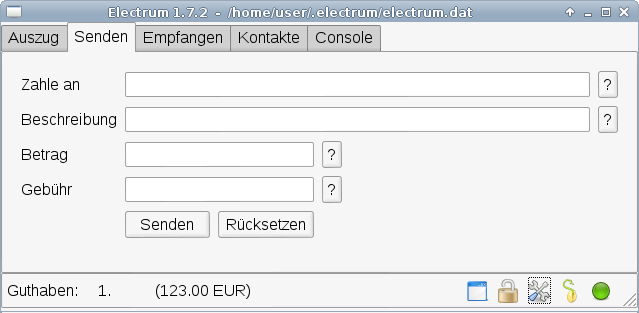
\includegraphics[scale=0.55]{../screenshots/electrum2.png}
\caption{Hauptfenster von Electrum}
\label{abb:electrummain}
\end{center}
\end{figure}

Die Oberfl�che ist einfach gehalten. F�r die �bersicht der Transaktionen, zum Senden und Empfangen sowie eine einfache Adressliste gibt es Reiter im Hauptfenster (Bild \ref{abb:electrummain}).\\

Alle Transaktionen werden in der Blockchain gespeichert. Sie k�nnen mit dem \textit{Seed} aus dem \textit{ewigen Logfile} rekonstruiert werden. Ein vollst�ndiges Backup der Konfiguration ist nicht n�tig. Man ben�tigt nur den Seed, der wie eine lange Passphrase aus zw�lf Worten besteht. F�r ein Backup des Seed klickt man auf zweite Symbol von rechts in der Statusleiste und speichert die Passphrase (z.B. in einer verschl�sselten Passwortdatenbank wie KeepassX). Mit dem QR-Code kann man den Seed schnell auf ein Smartphone �bertragen.\\

\begin{figure}[tb]
\begin{center}
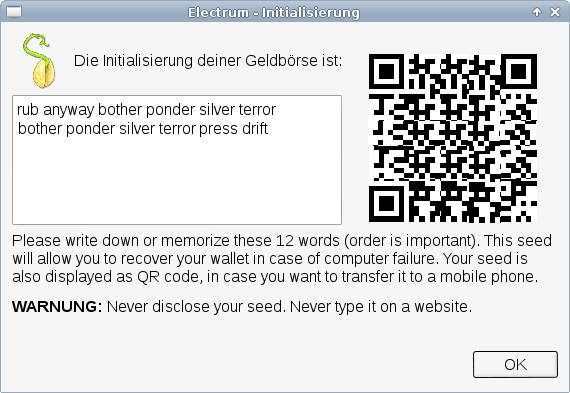
\includegraphics[scale=0.55]{../screenshots/electrum3.png}
\caption{Seed exportieren}
\label{abb:electrumseed}
\end{center}
\end{figure}

Die Netzwerkeinstellungen �ffnet man mit einem Klick auf das rechte Icon in der Statusleiste, dass �blicherweise ein gr�ner Punkt ist. Hier kann man festlegen, welchen Server man f�r die rechenintensiven Aufgaben nutzen m�chte. Der Server kann aus der Liste frei gew�hlt werden. Es werden keine Accountdaten auf dem Server gespeichert.\\

Au�erdem kann man in den Netzwerkeinstellungen den Proxy konfigurieren. Da Electrum nur geringen Datenverkehr verursacht, ist eine sinnvolle Kombination mit den Anonymisierungs�diensten Tor oder JonDonym m�glich. Das verhindert eine zuk�nftige Deanonymiserung des Nutzers durch Analyse des ewigen Logfiles. Die Proxy Einstellungen k�nnen auch beim Start des Programms als Parameter �bergeben werden:
\begin{itemize}
 \item Um den Datenverkehr von Electrum mit den Premiumdiensten von JonDonym zu anonymisieren, startet man das Programm mit folgenden Proxy-Parametern:
 \begin{verbatim}
    electrum --proxy=http:127.0.0.1:4001
 \end{verbatim} 
 \item Wenn man Tor Onion Router nutzen m�chte (TorBrowserBundle), dann nimmt man:
 \begin{verbatim}
    electrum --proxy=socks5:127.0.0.1:9150
 \end{verbatim}
\end{itemize}

Die Server f�r den rechenintensiven Part werden durch Spenden finanziert. Die Betreiber sind f�r eine kleine Spende in Bitcoins dankbar. Die Spendenadresse f�r den aktuell genutzten Server findet man auf dem Reiter \textit{Console} im Hauptfenster.

\subsection{Anonymit�t von Bitcoin}
�ber die Anonymit�t von Bitcoin gibt es viele Missverst�ndnisse. So wie jeder Geldschein eine eindeutige Nummer hat und verfolgt werden kann, ist es einem potenten Beobachter auch m�glich, Bitcoin Zahlungen zu verfolgen.\\

Alle Bitcoin Transaktionen werden im \textit{ewigen Logfile} protokolliert, das �ffentlich zug�nglich ist. Das ist kein Designfehler sondern notwendig, um double spending zu verhindern. Forscher der TU Darmstadt haben auf dem 28C3 eine Analyse des \textit{ewigen Logfile} von Bitcoin vorgestellt \footnote{ \href{http://events.ccc.de/congress/2011/Fahrplan/events/4746.en.html}{http://events.ccc.de/congress/2011/Fahrplan/events/4746.en.html}}. Eine weitere Analyse wurde von D. Ron und A. Shamir publiziert \footnote{ \href{http://eprint.iacr.org/2012/584}{http://eprint.iacr.org/2012/584}}. Beide Analysen konnten scheinbar unabh�ngige Bitcoin Adressen zusammen f�hren und die IP-Adressen von Nutzern ermitteln. Dazu z�hlen beispielsweise Spender, die an Wikileaks via Bitcoin gespendet haben. Au�erdem wurden Zahlen zur Bitcoin Nutzung von Wikileaks als Beispiel ver�ffentlicht. Bis M�rz 2012 nutzte Wikileaks 83 Bitcoin Adressen und erhielt 2605.25 BTC von Unterst�tzern.\\

Die Forscher kommen zu dem Schluss, dass die Anonymit�t von Bitcoin geringer ist, als eine einfache Bank�berweisung. Informationen zu Bank�berweisungen kann man nicht \textit{einfach so} bekommen. as Bankgeheimnis verwehrt vielfach den Zugriff auf die Konto�informationen. Die Bitcoin Transaktionen kann jeder analysieren, der �ber die n�tige Rechenleistung verf�gt.\\

Die CIA hat nach eigenen Aussagen Bitcoin als Zahlungsmittel \textit{bereits auf dem Radar}. Im Juni 2011 wurde Gavin Andresen (ein f�hrender Bitcoin Entwickler) ins CIA-Haupquartier zu einer Pr�sentation eingeladen. Auch das US-Milit�r sucht(e) bereits einen Anti-Terror Finanzexperten mit Bitcoin Erfahrung. Die Europ�ische Zentralbank (EZB) sieht laut einem Bericht von Okt. 2012 in Bitcoin eine Gefahr, da es au�erhalb der Kontrolle der Zentralbanken l�uft. Die EZB empfiehlt eine intensivere Beobachtung. Es gibt also viele Gr�nde, m�glichst anonym zu bleiben.

\subsubsection*{Bitcoin anonym nutzen}
Da der gesamte System von Bitcoin auf Informationsaustausch im Internet basiert, ist es mit Anonymisierungsdiensten m�glich, Bitcoin auch vollst�ndig anonym zu nutzen. Dabei sind folgende Punkte zu beachten:

\begin{description}
 \item[Bitcoin-Brieftasche anonym verwalten:] 
  Man kann einen Webservice verwenden und mit den Anonymisierungs�diensten \textit{JonDo+JonDoFox} oder dem \textit{TorBrowserBundle} das eWallet anonym auf den Servern verwalten.
 \begin{itemize}
  \item Blockchain.info\footnote{ \href{https://www.blockchain.info/wallet}{https://www.blockchain.info/wallet}} bietet die Verwaltung eines anonymen eWallet auf dem Webserver und erfordert keine pers�nlichen Angaben bei der Registrierung.
  \item StrongCoin.com\footnote{ \href{https://www.strongcoin.com}{https://www.strongcoin.com}} erfordert die Angabe einer E-Mail Adresse bei der Registrierung. Wegwerfadressen werden akzeptiert. Das Webinterface ist f�r Smartphones geeignet.
  \item OnionBC ist ein anonymer eWallet Service, der nur als Tor Hidden Service unter \href{http://6fgd4togcynxyclb.onion/}{6fgd4togcynxyclb.onion} erreichbar ist. (Ich bin immer etwas skeptisch bei Tor Hidden Services. Wenn man nicht weiss, wer den Dienst betreibt, kann es sich oft um Scam handeln. TORwallet hat sich z.B. als Scam herausgestellt.)
 \end{itemize}
 
Wenn man einem Webdienst nicht vertrauen m�chte, kann man den Bitcoin Client \textit{Electrum}\footnote{ \href{http://electrum.org/index.html}{http://electrum.org}} installieren und den Datenverkehr mit Tor oder JonDonym anonymisieren. Electrum �ber�l�sst die Hauptarbeit speziellen Servern und muss deshalb nicht das \textit{ewige Logfile} st�ndig aktualisieren. Das reduziert den Datenverkehr und erm�glicht eine sinnvolle Kombination mit JonDonym oder Tor. Die privaten Schl�ssel bleiben aber immer auf dem eigenen Rechner.\\

Um den Datenverkehr von Electrum mit den Premiumdiensten von JonDonym zu anonymisieren, startet man das Programm mit folgenden Proxy-Parametern:
\begin{verbatim}
    electrum --proxy=http:127.0.0.1:4001
\end{verbatim} 
Wenn man Tor Onion Router nutzen m�chte (TorBrowserBundle), dann startet man das Programm mit folgenden Proxy-Parametern:
\begin{verbatim}
    electrum --proxy=socks5:127.0.0.1:9150
\end{verbatim} 
Die Installation von JonDo oder Tor ist im Kapitel \textit{Anonymisierungsdienste} beschrieben.

\item[Bitcoins anonym kaufen:]
Man kann beim Kauf von Bitcoins die Angabe eines Bankkontos oder anderer identifizierender Informationen vermeiden.
\begin{itemize}
 \item Auf der Webseite LocalBitcoins.com\footnote{ \href{https://localbitcoins.com/}{https://localbitcoins.com/}} findet man weitere Anbieter in der Umgebung, die Bitcoins gegen Cash mit pers�nlicher Geld�bergabe verkaufen.
 \item Im IRC Channel \#bitcoin-otc im Freenode Netz kann man beliebige Formen der Geld�bergabe mit dem Verk�ufer vereinbaren.
 \item In Berlin trifft sich die Bitcoin Community an jedem ersten Donnerstag im Monat im \textit{room 77} (Graefestr. 77, 10967 Berlin-Kreuzberg). Dort findet immer jemanden, der Bitcoins gegen Bargeld verkauft.
 \item Wer den Anonymisierungsdienst JonDonym nutzt, kann im Bitcoin Shop der JonDos GmbH \footnote{ \href{https://shop.anonymous-proxy-servers.net/bin/btc-shop}{https://shop.anonymous-proxy-servers.net/bin/btc-shop}} anonym kaufen und mit Paysafecard bezahlen (wenn Coins im Shop vor�handen sind). Damit kann man auch Restbetr�ge von Paysafecards verwenden.
\end{itemize}

\item[Bitcoins als Zahlungsmittel verwenden:]
 Beim Einkauf virtueller G�ter (z.B. JonDonym Premium Codes oder eBooks, die per E-Mail zugestellt werden) gibt es keine weiteren Probleme. Muss man beim Kauf realer G�ter eine Lieferadresse angeben, dann sollte man ein anderes Bitcoin eWallet verwenden als f�r die anonyme Bezahlung virtueller G�ter. Anderenfalls k�nnten auch  die anonymen Zahlungen deanonymisiert werden.\\

\item[Mixing-Services?] Im Bitcoin-Wiki werden Mixing-Services wie Blockchain Mixing Service\footnote{ \href{https://blockchain.info/wallet/send-anonymously}{https://blockchain.info/wallet/send-anonymously}} oder Cleanbit.org\footnote{ \href{http://www.cleanbit.org/}{http://www.cleanbit.org/}} empfohlen, um die Spuren einer Transaktion zu verwischen. Die Analyse von D. Ron und A. Shamir l�sst vermuten, dass diese Mixing-Services mit entsprechendem Aufwand analysiert werden k�nnten und zuk�nftig einen potenten Angreifer nicht von einer Verfolgung der Transaktionen abhalten k�nnen.

 \end{description}
 
\section{Bitcoin}
Bitcoin ist eine digitale Peer-2-Peer W�hrung ohne zentrale Verwaltung. Sie ist unabh�ngig von der Geldpolitik einer Zentralbank und entwickelt sich marktgetrieben durch die Aktivit�ten der Teilnehmer, die Bitcoin als Zahlungsmittel akzeptieren oder verwenden.\\

Die Wurzeln der �konomischen Theorie dieser virtuellen W�hrung liegen in der \textit{Austrian school of economics}, die von den �konomen Eugen v. B�hm-Bawerk, Ludwig Mises und Friedrich A. Hayek entwickelt wurde. Die �konomen kritisieren das gegenw�rtige System des Fiatgeldes der Zentralbanken. Sie sehen in den massiven, politisch motivierten Interventionen der Zentralbanken in den Geldumlauf eine wesentliche Ursache f�r den Krisenzyklus. Als Ausweg empfehlen sie eine Internationalisierung der W�hrungen und die R�ckkehr zum Goldstandard.\\

Gegenw�rtig ist Bitcoin die popul�rste Umsetzung einer W�hrung in Anlehnung an die Konzepte der \textit{Austrian school of economics}. Die Software l�st mit kryptografischen Methoden vor allem zwei Probleme:

\begin{enumerate}
 \item Das Kopieren und mehrfache Verwendung der Bits und Bytes, die ein Coin repr�sentieren, ist nicht m�glich.
 \item Die Gesamtmenge der verf�gbaren Coins ist limitiert. Neue Bitcoins werden nach einem festen Schema generiert und die Gesamtzahl ist limitiert.
\end{enumerate}

Darauf aufbauend kann Bitcoin als Bezahlmethode verwendet werden. Bitcoins lassen sich in reale W�hrungen hin- und zur�cktauschen. Der Kurswert der Bitcoins beim Tausch gegen reale W�hrungen (z.B. Euro) ergibt sich dabei ausschlie�lich aus dem Markt. Die Bezahlungen k�nnen relativ schnell am PC abgewickelt werden. Es dauert in der Regel nur 1-2h, bis das Bitcoin Netzwerk eine Transaktion hinreichend best�tigt hat.\\

Viele Dienste im Netz akzeptieren Bitcoins als Bezahlung. Eine �bersicht findet man im Bitcoin Wiki \footnote{ \href{https://en.bitcoin.it/wiki/Trade}{https://en.bitcoin.it/wiki/Trade}}. Man kann Musik, E-Books, Web- und Mailhosting oder Anonymisierungsdienste / VPN-Anbieter mit Bitcoins bezahlen. Der Kurs wird dabei von jedem Anbieter selbst festgelegt. Dabei kann es vorkommen, dass Anbieter vom mittleren Tauschkurs abweichen.\\

Um mit Bitcoins zu bezahlen, braucht man selbst ein paar Bitcoins. Diese kann man auf verschiedenen Markpl�tzen gegen reale W�hrung kaufen oder man bietet selbst Dienst�leistungen gegen Bitcoins als Bezahlung an. Die Markpl�tze dienen dabei nur zur Anbahnung der Transaktionen \textit{Geld gegen Bitcoin}. Der Austausch des reales Geldes erfolgt in der Regel auf direktem Weg zwischen den Beteiligten.\\

\subsection{Exchanger / Marktpl�tze}
Man kann Bitcoin komplett ohne Installation einer Software nutzen. Es gibt Webdienste (die sogenannten Exchanger oder Markpl�tze), die den Handel mit Bitcoins zwischen den Personen einleiten und eine Bitcoin Brieftasche (eWallet) f�r Nutzer bereitstellen. Das vereinfacht die Nutzung von Bitcoin als Zahlungsmittel, da eine Installation von Software nicht zwingend n�tig ist. Die erworbenen Bitcoins k�nnen aber auch auf den eigenen PC transferiert und mit einem Bitcoin Client verwaltet werden.\\

Die Exchanger verifizieren die Identit�t der Nutzer. Eine anonyme Nutzung ist nicht m�glich. Hinweise zum anonymen Kauf von Bitcoins findet man weiter unten im Abschnitt \textit{Anonymit�t von Bitcoin}.\\

Eine �bersicht zu den Marktpl�tzen findet man auch im Bitcoin Wiki \footnote{ \href{https://en.bitcoin.it/wiki/Buying\_bitcoins}{https://en.bitcoin.it/wiki/Buying\_bitcoins}}. F�r den Einstieg gef�llt mir \textbf{\href{https://www.bitcoin.de}{www.bitcoin.de}} sehr gut. Die Webseite wird professionell betreut, bietet in einer �ber�sichtlichen Struktur alle n�tigen Informationen f�r Kaufen, Verkaufen und die Verwaltung der eigene Bitcoins und ist f�r die ersten Schritte gut geeignet. Allerdings ist der Dienst nicht ganz kostenfrei. Es wird eine Geb�hr von 1\% f�r den Handel mit Bitcoins erhoben.\\

Die Anmeldung bei Bitcoin.de erfordert die Angabe einer E-Mail Adresse und einer Bank�verbindung. Die Bankverbindung wird durch eine einmalige �berweisung von 1 Cent verifiziert. Tempor�re E-Mail Adressen sollten nicht genutzt werden, da bei jeder Transaktion Informationen per Mail gesendet werden. Man kann zus�tzliche die Zahlungsm�glichkeiten Liberty Reserve und Money Bookers nutzen.\\ 

\textbf{Bitcoins kaufen:} Im Markbereich stehen in einer Liste mehrer Verkaufsangebote. Durch Klick auf den Link \textit{Kaufen} kann man ein Kaufangebot annehmen. Sie erhalten ein E-Mail mit den Daten f�r die Bezahlung. �berweisen Sie dem Verk�ufer das Geld und best�tigen Sie die �berweisung auf der Webseite innerhalb von 12h. Wenn der Verk�ufer den Zahlungseingang best�tigt, erhalten Sie die Bitcoins. Wenn kein passendes Angebot zu finden ist, k�nnen Sie ein Kaufangebot einstellen und auf Angebote warten.\\

Der K�ufer sendet dem Verk�ufer den Kaufpreis abz�glich 0.5\% und erhalten daf�r Bitcoins abz�glich 1\% des Kaufangebotes. Somit teilen sich K�ufer und Verk�ufer die Marktgeb�hr von 1\% jeweils zur H�lfte. Ein Rechenbespiel: 
\begin{itemize}
 \item Das Angebot lautet: 1 BTC f�r 40,00 Euro.
 \item Der K�ufer �berweist 39,80 Euro an den Verk�ufer.
 \item Er erh�lt daf�r 0,99 BTC auf seinem Konto.
\end{itemize}

Die f�r ihre Transaktion g�ltigen Zahlen werden jeweils bei Annahme des Kaufangebotes und in der E-Mail angezeigt. Die Kontodaten des Verk�ufers erhalten Sie ebenfalls per E-Mail.\\

\subsection{Bitcoin Software}
Wenn man einem externen Webserver nicht vertraut, kann man seine Bitcoins lokal auf dem eigenen Rechner oder Smartphone verwalten. Daf�r muss ein Bitcoin Client wie Bitcoin-Qt oder Electrum installiert werden.

\begin{description}
 \item[Bitcoin-Qt] ist der Standard Client des Bitcoin Projektes und steht zum Download unter \href{http://bitcoin.org/en/download}{http://bitcoin.org/en/download} bereit. Er ist einfach bedienbar, bietet eine �bersicht �ber alle Transaktionen und kann beliebig viele Adressen verwalten.\\

Ein Nachteil f�r Gelegenheitsnutzer ist der st�ndige Download der gesamten Blockchain. Die Down�load�seite weist darauf hin, dass die erste Initialisierung bis zu einem Tag dauern kann. Wenn man nach 3-4 Wochen Pause wieder einmal mit Bitcoins bezahlen m�chte, dann ben�tigt Bitcoin-Qt ein bis zwei Stunden f�r die Aktualisierung der Blockchain, um wieder arbeitsbereit zu werden.

 \item[Electrum] ist eine leichtgewichtige Alternative f�r Gelegenheitsnutzer. Er �berl�sst die Hauptarbeit speziellen Servern im Netz und ben�tigt die komplette Blockchain nicht. Trotzdem ist sichergestellt, dass die privaten Schl�ssel ausschlie�lich in der Verf�gung des Anwenders liegen. Die Installation f�r unterschiedliche Betriebssysteme ist auf der Down�load�seite  \href{http://electrum.org/download.html}{http://electrum.org/download.html} beschrieben.\\

\begin{figure}[tb]
\begin{center}
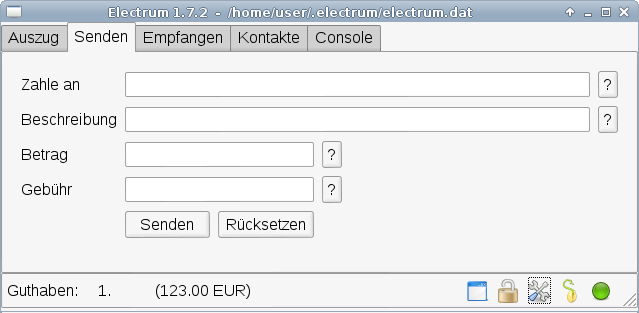
\includegraphics[scale=0.55]{../screenshots/electrum2.png}
\caption{Hauptfenster von Electrum}
\label{abb:electrummain}
\end{center}
\end{figure}

Die Oberfl�che ist einfach gehalten. F�r die �bersicht der Transaktionen, zum Senden und Empfangen sowie eine einfache Adressliste gibt es Reiter im Hauptfenster (Bild \ref{abb:electrummain}).\\

Alle Transaktionen werden in der Blockchain gespeichert. Sie k�nnen mit dem \textit{Seed} aus diesem \textit{ewigen Logfile} rekonstruiert werden. Ein vollst�ndiges Backup der Konfiguration ist nicht n�tig. Man ben�tigt nur den Seed, der wie eine lange Passphrase aus zw�lf Worten besteht. F�r ein Backup des Seed klickt man auf zweite Symbol von rechts in der Statusleiste und speichert die Passphrase (z.B. in einer verschl�sselten Passwortdatenbank wie KeepassX). Mit dem QR-Code kann man den Seed schnell auf ein Smartphone �bertragen.\\

\begin{figure}[tb]
\begin{center}
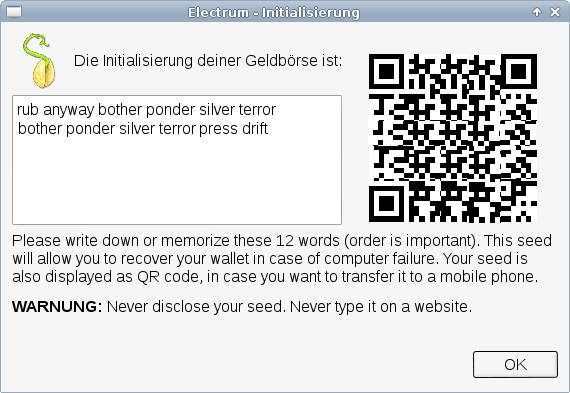
\includegraphics[scale=0.55]{../screenshots/electrum3.png}
\caption{Seed exportieren}
\label{abb:electrumseed}
\end{center}
\end{figure}

Die Netzwerkeinstellungen �ffnet man mit einem Klick auf das rechte Icon in der Statusleiste, dass �blicherweise ein gr�ner Punkt ist. Hier kann man festlegen, welchen Server man f�r die rechenintensiven Aufgaben nutzen m�chte. Der Server kann aus der Liste frei gew�hlt werden, da keine Accountdaten auf dem Server gespeichert werden. Die Server werden durch Spenden finanziert und die Betreiber sind f�r eine kleine Spende in Bitcoins dankbar. Die Spendenadresse f�r den aktuell genutzten Server findet man auf dem Reiter \textit{Console} im Hauptfenster.\\

Au�erdem kann man in den Netzwerkeinstellungen den Proxy konfigurieren. Da Electrum nur geringen Datenverkehr verursacht, ist eine sinnvolle Kombination mit den Anonymisierungs�diensten Tor oder JonDonym m�glich. Das verhindert eine zuk�nftige Deanonymiserung des Nutzers durch Analyse des ewigen Logfiles. Die Proxy Einstellungen k�nnen auch beim Start des Programms als Parameter �bergeben werden:
\begin{itemize}
 \item Um den Datenverkehr von Electrum mit den Premiumdiensten von JonDonym zu anonymisieren, startet man das Programm mit folgenden Proxy-Parametern:
 \begin{verbatim}
    electrum --proxy=http:127.0.0.1:4001
 \end{verbatim} 
 \item Wenn man Tor Onion Router nutzen m�chte (TorBrowserBundle), dann nimmt man:
 \begin{verbatim}
    electrum --proxy=socks5:127.0.0.1:9150
 \end{verbatim}
\end{itemize}

\end{description}

\subsection{Anonymit�t von Bitcoin}
�ber die Anonymit�t von Bitcoin gibt es viele Missverst�ndnisse. So wie jeder Geldschein eine eindeutige Nummer hat und verfolgt werden kann, ist es einem potenten Beobachter auch m�glich, Bitcoin Zahlungen zu verfolgen.\\

Alle Bitcoin Transaktionen werden in der �ffentlich zug�glichen Blockchain protokolliert (ein \textit{ewiges Logfiles}). Das ist kein Designfehler sondern notwendig, um double spending zu verhindern. Forscher der TU Darmstadt haben auf dem 28C3 eine Analyse des \textit{ewigen Logfile} von Bitcoin vorgestellt \footnote{ \href{http://events.ccc.de/congress/2011/Fahrplan/events/4746.en.html}{http://events.ccc.de/congress/2011/Fahrplan/events/4746.en.html}}. Eine weitere Analyse wurde von D. Ron und A. Shamir publiziert \footnote{ \href{http://eprint.iacr.org/2012/584}{http://eprint.iacr.org/2012/584}}. Beide Analysen konnten scheinbar unabh�ngige Bitcoin Adressen zusammen f�hren und die IP-Adressen von Nutzern ermitteln. Dazu z�hlen beispielsweise Spender, die an Wikileaks via Bitcoin gespendet haben. Au�erdem wurden Zahlen zur Bitcoin Nutzung von Wikileaks als Beispiel ver�ffentlicht. Bis M�rz 2012 nutzte Wikileaks 83 Bitcoin Adressen und erhielt 2605.25 BTC von Unterst�tzern.\\

Die Forscher kommen zu dem Schluss, dass die Anonymit�t von Bitcoin geringer ist, als eine einfache Bank�berweisung. Informationen zu Bank�berweisungen kann man nicht \textit{einfach so} bekommen. Das Bankgeheimnis verwehrt den Zugriff auf die Konto�informationen. Die Bitcoin Transaktionen kann jeder analysieren, der �ber die n�tige Rechenleistung verf�gt.\\

Die CIA hat nach eigenen Aussagen Bitcoin als Zahlungsmittel \textit{bereits auf dem Radar}. Im Juni 2011 wurde Gavin Andresen (ein f�hrender Bitcoin Entwickler) ins CIA-Haupquartier zu einer Pr�sentation eingeladen. Das US-Milit�r sucht(e) bereits Anti-Terror Finanzexperten mit Bitcoin Erfahrung. Die Europ�ische Zentralbank (EZB) sieht laut einem Bericht von Okt. 2012 in Bitcoin eine Gefahr, da es au�erhalb der Kontrolle der Zentralbanken l�uft. Die EZB empfiehlt eine intensivere Beobachtung. Es gibt also viele Gr�nde, m�glichst anonym zu bleiben.\\

Da das gesamte System von Bitcoin auf Informationsaustausch im Internet basiert, ist es mit Anonymisierungsdiensten m�glich, Bitcoin auch vollst�ndig anonym zu nutzen. Dabei sind folgende Punkte zu beachten:

\begin{description}
 \item[Bitcoin-Brieftasche anonym verwalten:] 
  Man kann einen Webservice verwenden und mit den Anonymisierungs�diensten \textit{JonDo+JonDoFox} oder dem \textit{TorBrowserBundle} das eWallet anonym auf den Servern verwalten.
 \begin{itemize}
  \item Blockchain.info\footnote{ \href{https://www.blockchain.info/wallet}{https://www.blockchain.info/wallet}} bietet die Verwaltung eines anonymen eWallet auf dem Webserver und erfordert keine pers�nlichen Angaben bei der Registrierung.
  \item StrongCoin.com\footnote{ \href{https://www.strongcoin.com}{https://www.strongcoin.com}} erfordert die Angabe einer E-Mail Adresse bei der Registrierung. Wegwerfadressen werden akzeptiert. Das Webinterface ist f�r Smartphones geeignet.
  \item OnionBC ist ein anonymer eWallet Service, der nur als Tor Hidden Service unter \href{http://6fgd4togcynxyclb.onion/}{6fgd4togcynxyclb.onion} erreichbar ist. (Ich bin immer etwas skeptisch bei Tor Hidden Services. Wenn man nicht weiss, wer den Dienst betreibt, kann es sich oft um Scam handeln. TORwallet hat sich z.B. als Scam herausgestellt.)
 \end{itemize}
 
Wenn man einem Webdienst nicht vertrauen m�chte, kann man den Bitcoin Client \textit{Electrum}\footnote{ \href{http://electrum.org/index.html}{http://electrum.org}} installieren und den Datenverkehr mit Tor oder JonDonym anonymisieren. Electrum �ber�l�sst die Hauptarbeit speziellen Servern und muss deshalb nicht das \textit{ewige Logfile} st�ndig aktualisieren. Das reduziert den Datenverkehr und erm�glicht eine sinnvolle Kombination mit JonDonym oder Tor. Die privaten Schl�ssel bleiben aber immer auf dem eigenen Rechner.\\

Um den Datenverkehr von Electrum mit den Premiumdiensten von JonDonym zu anonymisieren, startet man das Programm mit folgenden Proxy-Parametern:
\begin{verbatim}
    electrum --proxy=http:127.0.0.1:4001
\end{verbatim} 
Wenn man Tor Onion Router nutzen m�chte (TorBrowserBundle), dann startet man das Programm mit folgenden Proxy-Parametern:
\begin{verbatim}
    electrum --proxy=socks5:127.0.0.1:9150
\end{verbatim} 
Die Installation von JonDo oder Tor ist im Kapitel \textit{Anonymisierungsdienste} beschrieben.

\item[Bitcoins anonym kaufen:]
Man kann beim Kauf von Bitcoins die Angabe eines Bankkontos oder anderer identifizierender Informationen vermeiden.
\begin{itemize}
 \item Auf der Webseite LocalBitcoins.com\footnote{ \href{https://localbitcoins.com/}{https://localbitcoins.com/}} findet man Anbieter in der Umgebung, die Bitcoins gegen Bargeld verkaufen.
 \item Im IRC Channel \#bitcoin-otc im Freenode Netz kann man beliebige Formen der Geld�bergabe mit dem Verk�ufer vereinbaren.
 \item In Berlin trifft sich die Bitcoin Community an jedem ersten Donnerstag im Monat im \textit{room 77} (Graefestr. 77, 10967 Berlin-Kreuzberg). Dort findet immer jemanden, der Bitcoins gegen Bargeld verkauft.
 \item Wer den Anonymisierungsdienst JonDonym nutzt, kann im Bitcoin Shop der JonDos GmbH \footnote{ \href{https://shop.anonymous-proxy-servers.net/bin/btc-shop}{https://shop.anonymous-proxy-servers.net/bin/btc-shop}} kaufen und mit Paysafecard bezahlen. Damit kann man auch Restbetr�ge von Paysafecards verwenden.
\end{itemize}

\item[Bitcoins als Zahlungsmittel verwenden:]
 Beim Einkauf virtueller G�ter (z.B. JonDonym Premium Codes oder eBooks, die per E-Mail zugestellt werden) gibt es keine weiteren Probleme.\\

Muss man beim Kauf realer G�ter eine Lieferadresse angeben, dann sollte man ein anderes Bitcoin eWallet verwenden als f�r die anonyme Bezahlung virtueller G�ter. Anderenfalls k�nnten auch  die anonymen Zahlungen deanonymisiert werden.\\

\item[Mixing-Services?] Im Bitcoin-Wiki werden Mixing-Services wie Blockchain Mixing Service\footnote{ \href{https://blockchain.info/wallet/send-anonymously}{https://blockchain.info/wallet/send-anonymously}} oder Cleanbit.org\footnote{ \href{http://www.cleanbit.org/}{http://www.cleanbit.org/}} empfohlen, um die Spuren einer Transaktion zu verwischen. Die Analyse von D. Ron und A. Shamir l�sst vermuten, dass diese Mixing-Services mit entsprechendem Aufwand analysiert werden k�nnten und zuk�nftig einen potenten Angreifer nicht von einer Verfolgung der Transaktionen abhalten k�nnen.

 \end{description}
 

\chapter{Allgemeine Hinweise zur E-Mail Nutzung}
E-Mail ist eines der meistgenutzten Kommunikationsmittel. Die folgenden Seiten sollen zum Nachdenken �ber die die Auswahl des E-Mail Providers anregen und Hinweise f�r die Konfiguration von Mozilla Thunderbird geben.

\section{E-Mail Provider}
Als erstes braucht man eine oder mehrere E-Mail Adressen. Es ist empfehlenswert, f�r unter�schiedliche Anwendungen auch verschiedene E-Mail Adressen zu verwenden. Es erschwert die Profilbildung anhand der E-Mail Adresse und verringert die Spam-Bel�stigung. Wenn Amazon, Ebay oder andere kommerzielle Anbieter zu aufdringlich werden, wird die mit Spam �ber�schwemmte E-Mail Adresse einfach gel�scht ohne die private Kommunikation zu st�ren.\\

Neben einer sehr privaten E-Mail Adresse f�r Freunde k�nnte man weitere E-Mail Adressen f�r Eink�ufe im Internet nutzen oder f�r politische Aktivit�ten. Um nicht st�ndig viele E-Mail Accounts abfragen zu m�ssen, kann man die f�r Eink�ufe im Internet genutzt E-Mail Accounts auch an die private Hauptadresse weiterleiten lassen. Alle Mail-Provider bieten diese Option. Bei den gro�en deutschen Mail Providern GMX.de und WEB.de gibt es bis zu 100 Fun-Domains extra f�r diesen Zweck. Bereits mit der kostenlosen Version kann man bis zu 3 Fun-Adressen nutzen.\\ 

Wenn eine E-Mail Adresse nur f�r die Anmeldung in einem Forum oder das Ver�ffentlichen eines Kommentars in Blogs ben�tigt wird, kann man \textit{tempor�re Mailadressen} nutzen (siehe weiter unten).\\

Eine kleine Liste von E-Mail Providern abseits des Mainstream:
\begin{itemize}
 \item \textbf{Posteo.de} \footnote{ \href{https://posteo.de/}{https://posteo.de}} und \textbf{aikQ.de} \footnote{ \href{https://www.aikq.de/}{https://www.aikq.de}} (deutsche Mailprovider, Accounts ab 1,- Euro pro Monat, anonyme Accounts m�glich mit Bezahlung per Brief)
 \item \textbf{VFEmail} \footnote{ \href{https://www.vfemail.net/}{https://www.vfemail.net}} (anonymer Mailprovider, ben�tigt eine Wegwerf-Adresse f�r Registrierung, kostenfreie Accounts mit POP3/SMTP und beliebig vielen tempor�ren E-Mail Adressen)
 \item \textbf{CryptoHeaven} \footnote{ \href{https://www.cryptoheaven.com/index.shtml}{https://www.cryptoheaven.com/}} (Accounts ab \$60 pro Jahr, einfache Verschl�sselung der Kommunikation mit Accounts beim gleichen Provider, Offshore registrierte Firma, Server in Kanada)
 \item \textbf{XMAIL.net} \footnote{ \href{https://www.xmail.net}{https://www.xmail.net}} (die Betreiberfirma Aaex Corp. ist auf den British Virgin Islands registriert, die Server stehen in Kanada, kostenfrei Accounts mit POP3, aber ohne SMTP)
 \item \textbf{runbox.com} \footnote{ \href{https://secure.runbox.com/}{https://secure.runbox.com/}} (norwegischer E-Mail Provider, Server stehen ebenfalls in Norwegen, Accounts ab 1,66 Dollar pro Monat)
 \item \textbf{neomailbox.com} \footnote{ \href{http://www.neomailbox.com/services/secure-email}{http://www.neomailbox.com/services/secure-email}} (anonymes E-Mail Hosting in der Schweiz, Accounts ab 3,33 Dollar pro Monat, anonyme Bezahlung mit Pecunix oder Liberty Reserve m�glich)
\end{itemize}

F�r politische Aktivisten gibt es Anbieter, die insbesondere den Schutz vor staatlichem Zugriff hervorheben. Diese Anbieter werden mit Spenden finanziert. F�r einen Account muss man seine politischen Aktivit�ten nachweisen, aber nicht unbedingt seine Identit�t offen legen. Neben E-Mail Accounts werden auch Blogs und Mailinglisten angeboten.
\begin{itemize}
 \item \textbf{Associazione-Investici} \footnote{ \href{http://www.autistici.org/de/get\_service.html}{http://www.autistici.org/de/get\_service.html}} (italienischer Provider, Server stehen bei XS4ALL in Niederlande, verwendet eigene Certification Authority f�r SSL-Zertifikate)
 \item \textbf{Nadir.org} \footnote{ \href{http://www.nadir.org/}{http://www.nadir.org}} (deutscher Provider, Server stehen ebenfalls bei XS4ALL)
 \item \textbf{AktiviX.org} \footnote{ \href{https://www.aktivix.org/}{https://www.aktivix.org}} (deutscher Provider, Server stehen in Brasilien)
\end{itemize}

Hinweis: es kostet Geld, einen zuverl�ssigen Mailservice bereitzustellen. Es ist durchaus sinnvoll, die \textit{alles kostenlos Mentalit�t} f�r einen vertrauensw�rdigen Mailprovider fallen zu lassen.

\subsubsection*{Webinterfaces der Mail-Provider sind oft unsicher}
Die Webinterfaces der Mail-Provider bieten �berwiegend eine unsichere Konfiguration der HTTPS-Verschl�sselung des Webinterface. Oft ist es f�r einen Angreifer m�glich, eine schwache, abh�rbare Verschl�sselung zu erzwingen. Insecure Renegotiation wird teilweise noch verwendet oder das veraltete SSLv2 wird noch unterst�tzt. Das Problem betrifft nicht nur die Webseiten der Mail-Provider. Nach einer Studie bieten nur 10\% der Websites sichere Verschl�sselung nach dem Stand der Technik.\footnote{ \href{http://www.heise.de/developer/meldung/SSL-Pulse-protokolliert-Sicherheit-von-Webseiten-1569214.html}{http://www.heise.de/developer/meldung/SSL-Pulse-protokolliert-Sicherheit-von-Webseiten-1569214.html}}\\

Die folgenden Provider wurden mit dem \textit{SSL-Test von Qualys SSL Labs}\footnote{ \href{https://www.ssllabs.com/ssltest/index.html}{https://www.ssllabs.com/ssltest}} �berpr�ft: 
\begin{itemize}
 \item Posteo: sichere HTTPS-Verschl�sselung
 \item aikQ: sichere HTTPS-Verschl�sselung
 \item neomailbox.com: sichere HTTPS-Verschl�sselung
 \item VFEmail: sichere HTTPS-Verschl�sselung mit aktuellen Browsern
 \item CryptoHeaven: schwache Verschl�sselung und SSLv2 unterst�tzt
 \item XMAIL.net: schwache Verschl�sselung und SSLv2 werden unterst�tzt
 \item Runbox.com Insecure Renegotiation, SSLv2 wird unterst�tzt
\end{itemize}
 
Aus diesem Grund sollte man einen E-Mail Client nutzen. Die Verschl�sselung f�r POP3 und SMTP ist bei den oben genannten Providern auf dem aktuellen Stand der Technik. Da viele E-Mail Provider POP3 und SMTP nur f�r Premium-Kunden anbieten, sollte man nicht an der falschen Stelle sparen und sich nicht mit einem kostenfreien Account via Webinterface begn�gen. 

\subsubsection*{Nicht empfohlene E-Mail Provider}
Einige Gr�nde, warum verschiedene E-Mail Provider mit gutem Ruf nicht in die Liste der Empfehlungen aufgenommen wurden:
\begin{itemize}
 \item Hushmail speichert zuviel Daten. Neben den �blichen Daten beim Besuch der Webseite werden die E-Mails gescannt und folgende Daten unbegrenzt lange gespeichert:
\begin{enumerate}
 \item alle Sender- und Empf�nger E-Mail Adressen (VDS-artig)
 \item alle Dateinamen der empfangenen und gesendeten Attachements
 \item Betreffzeilen aller E-Mails (nicht verschl�sselbar)
 \item URLs aus dem Text unverschl�sselter E-Mails
 \item ... and any other information that we deem necessary
\end{enumerate}
Diese Daten werden bei der K�ndigung eines Account NICHT gel�scht.\\

Bei der Bezahlung f�r einen Premium-Account werden die IP-Adresse des Kunden sowie Land, Stadt und PLZ an Dritte weitergeben. Au�erdem bindet Hushmail.com Dienste von Drittseiten ein. Die ID des Hushmail Account wird beim Besuch der Webseite nach dem Login an diese Drittseiten �bermittelt. F�r die Privacy-Policy dieser Drittseiten �bernimmt Hushmail.com keine Verantwortung.
\item In der EU-Studie \textit{Fighting cyber crime and protecting privacy in the cloud}\footnote{ \href{http://www.europarl.europa.eu/committees/en/studiesdownload.html?languageDocument=EN\&file=79050}{http://www.europarl.europa.eu/committees/en/studiesdownload.html?languageDocument=EN\&file=79050}} warnen die Autoren in Kapitel 5.4 (S. 48) vor Risiken bei der Speicherung von Daten in den USA. Aufgrund des \textit{US PATRIOT Act} (insbesondere S. 215ff) und der \textit{4. Erg�nzung des FISA Amendments Act} ist es f�r US-Beh�rden ohne juristische Kontrolle m�glich, die Kommunikation von Nicht-US-B�rgern zu beschn�ffeln. Dabei ist es unerheblich, ob der Cloud- bzw. E-Mail Provider eine US-Firma ist oder nicht. Es reicht nach Ansicht der Amerikaner, wenn die Server in den USA stehen.\\

Aus diesem Grund ist ein Server-Standort \textit{USA} f�r deutsche Nutzer eher ungeeignet. Das betrifft u.a. die E-Mail Provider SecureNym, S-Mail, Fastmail.fm, Lavabit, Rise-up.net...
\item Cotse, Yahoo! und AOL bietet keine sichere Verschl�sselung f�r die Kommunikation zwischen Mail-Server und E-Mail Client (Secure Renegotiation wird nicht f�r SMTP unterst�tzt, was seit seit 2009 als schwerer Fehler im SSL Protokoll eingestuft wird).
\item Weitere Beispiele werden auf der Webseite des Handbuches genannt.\footnote{ \href{https://www.awxcnx.de/handbuch\_31.htm}{https://www.awxcnx.de/handbuch\_31.htm}}
\end{itemize}

\section{Mozilla Thunderbird}
Informationen und Downloadm�glichkeiten f�r Mozilla Thunderbird stehen auf der deutschsprachigen Website des Projektes \footnote{ \href{http://www.mozilla.org/de/thunderbird/}{http://www.mozilla.org/de/thunderbird/}} f�r Windows, Linux und MacOS zur Verf�gung.\\

Linux Distributionen enthalten in der Regel Thunderbird. Mit der Paketverwaltung kann Thunderbird und die deutsche Lokalisierung komfortabel installiert und aktualisiert werden. Debian GNU/Linux bietet eine angepasste Version von Thunderbird unter dem Namen \textit{Icedove} (allerdings meist in einer veralteten Version). Das Mozilla Debian Team stellt eine aktuellere Version in einem separatem Repository und eine Anleitung\footnote{ \href{http://mozilla.debian.net/}{http://mozilla.debian.net/}} zur Installation bereit.\\

\subsection{Account erstellen}
Nach dem ersten Start von Thunderbird f�hrt ein Assistent durch die Schritte zur Einrichtung eines E-Mail Kontos. Nach Eingabe der E-Mail-Adresse sowie des Passwortes erkennt der Assistent die n�tigen Einstellungen f�r den Mailserver oft automatisch. Es k�nnen auch die Einstellungen eines bisher verwendeten Programms �bernommen werden. Bei der Einrichtung des E-Mail Account sollten einige Punkte beachtet werden.\\

Die Grafik im Bild \ref{abb:email_web} zeigt den Weg einer E-Mail vom Sender zum Empf�nger. In der Regel ist man nicht direkt mit dem Internet verbunden. Der Zugang erfolgt �ber ein Gateway des Providers oder der Firma.\\

\begin{figure}[htb]
\begin{center}
 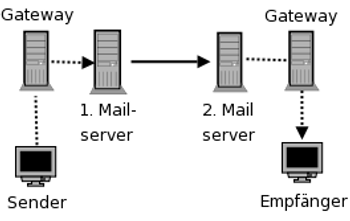
\includegraphics[scale=0.5]{../grafiken/email_weg.png}
\caption{Der Weg einer E-Mail durch das Web}
\label{abb:email_web}
\end{center}
\end{figure}

Der 1. Mailserver nimmt die E-Mail via SMTP entgegen und sendet sie an den 2. Mailserver. Hier liegt die E-Mail, bis der Empf�nger sie abruft und l�scht. Die gestrichelten Verbindungen zu den Mailservern k�nnen mit SSL bzw. TLS kryptografisch gesichert werden. Das hat nichts mit einer Verschl�sselung des Inhalts der E-Mail zu tun. Es wird nur die Daten�bertragung zum Mailserver verschl�sselt und es wird sichergestellt, dass man wirklich mit dem gew�nschten Server verbunden ist. Aktuelle Versionen von Thunderbird aktivieren dieses Feature beim Einrichten eines Account standardm��ig. \\

Wie einfach es ist, unverschl�sselte Verbindungen zu belauschen, die Passw�rter zu extrahieren und das Mail-Konto zu kompromittieren, wurde von T. Pritlove auf der re:publica 2007 demonstriert \footnote{ \href{http://tim.geekheim.de/2007/04/24/netzwerksicherheit-auf-der-republica/}{http://tim.geekheim.de/2007/04/24/netzwerksicherheit-auf-der-republica/}}.\\

Bewusst oder unbewusst k�nnen auch Provider die sichere �bertragung deaktivieren und damit den Traffic mitlesen. Es wird einfach die Meldung des Mail-Servers 250-STARTTLS gefiltert und �berschrieben. Scheinbar verf�gen alle DSL-Provider �ber die M�glichkeit, dieses Feature bei Bedarf f�r einzelne Nutzer zu aktivieren\footnote{ \href{http://heise.de/-206233}{http://heise.de/-206233}}. Die Standard-Einstellung der meisten E-Mail Clients ist \textit{``TLS verwenden wenn m�glich''}. Diese Einstellung ist genau in dem Moment wirkungslos, wenn man es braucht, weil der Traffic beschn�ffelt werden soll.\\

Alle brauchbaren Mail-Server bieten M�glichkeit der verschl�sselten Kommunikation via SSL/TLS oder STARTTLS. Diese Option ist in Thunderbird bei der Einrichtung eines neuen Kontos zu aktivieren. Der Assistent erledigt das in der Regel automatisch.\\

\begin{figure}[htb]
\begin{center}
 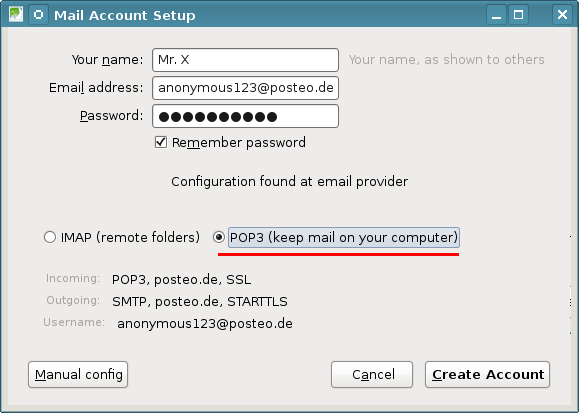
\includegraphics[scale=0.75]{../screenshots/thunderbird_account.png}
\caption{POP3-Account anlegen}
\label{abb:tbaccount1}
\end{center}
\end{figure}

SMTP, POP3 und IMAP sind f�r den Laien verwirrende Abk�rzungen.
\begin{description}
 \item[SMTP] ist das Protokoll zum Versenden von E-Mails.
 \item[POP3] ist das Protokoll zum Herunterladen von empfangenen E-Mails auf den lokalen Rechner. Dabei werden die E-Mails auf dem Server gel�scht.
 \item[IMAP] ist ein Kommunikationsprotokoll, um die empfangenen E-Mails auf dem Server zu verwalten und nur zum Lesen tempor�r herunter zu laden. Auch die versendeten E-Mails werden bei der Nutzung von IMAP auf dem Mailserver des Providers gespeichert.\\

 IMAP bietet damit die M�glichkeit, mit verschiedenen E-Mail Clients von unterschiedlichen Rechnern und Smartphones auf den Account zuzugreifen und stets Zugriff auf alle E-Mails zu haben. Die M�glichkeit des weltweiten Zugriffs auf seine Mails erkauft man sich aber mit Einschr�nkungen des Datenschutzes.\\

 Die auf dem Server des Providers gespeicherten E-Mails unterliegen NICHT mehr dem Tele�kommunikationsgeheimnis nach Artikel 10 GG, wenn der Nutzer Gelegenheit hatte, sie zu l�schen. Das BVerfG hat diese Rechtsauffassung 2009 in dem Urteil 2 BvR 902/06 best�tigt \footnote{ \href{https://www.bundesverfassungsgericht.de/pressemitteilungen/bvg09-079.html}{https://www.bundesverfassungsgericht.de/pressemitteilungen/bvg09-079.html}}.\\

 Mit der Reform der Telekommunikations�berwachung im Dezember 2012 k�nnen Geheim�dienste und Strafverfolge das Passwort f�r den Zugriff auf den Mail-Account ohne richter�liche Pr�fung vom Mail-Provider verlangen und damit Zugang zu dem Postfach erhalten. Es w�re unsch�n, wenn Sie dort die Kommunikation der letzten 5 Jahre vorfinden.
 \end{description}

Deshalb empfehle ich die Nutzung von POP3 (SSL) statt IMAP (Bild \ref{abb:tbaccount1}).\\

F�r viele E-Mail Provoder werden automatisch sichere Einstellungen vom Assistenten vorgeschlagen (SSL bzw. STARTTLS). Wenn keine Vorschl�ge gefunden werden k�nnen, kann man auf \textit{manuelle Konfiguration} klicken und in dem Dialog Bild \ref{abb:tbaccount2} die Einstellungen per Hand anpassen. Die n�tigen Daten f�r POP3- und SMTP-Server findet amn auf der Webseite des Mail-Providers. Au�erdem muss man in der Regel den Usernamen an die Vorgaben des Providers anpassen.
\begin{itemize}
 \item F�r den POP3-Server ist in der Regel Port \textit{995} (SSL) passend.
 \item Viele SMTP-Server bieten neben STARTTLS f�r Port \textit{25} auch auf den Ports \textit{587} (STARTTLS) oder Port \textit{465} (SSL) verschl�sselte Verbindungen zum Senden von E-Mails.
\end{itemize}

\begin{figure}[htb]
\begin{center}
 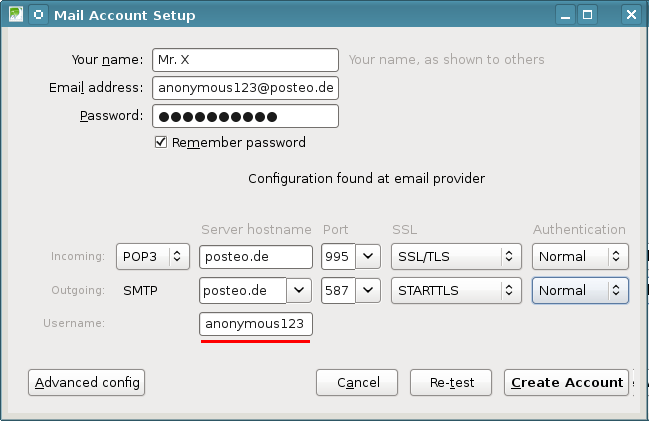
\includegraphics[scale=0.75]{../screenshots/thunderbird_account2.png}
\caption{POP3-Account anpassen}
\label{abb:tbaccount2}
\end{center}
\end{figure}

\subsection{Unsichere Verschl�sselungen deaktivieren}
Aus Gr�nden der Kompatibilt�t mit einigen Mail-Providern unterst�tzt Thunderbird noch immer veraltete und unsichere Verschl�sselungsoptionen f�r die Verbindung zu dem Mailservern. In den \textit{Erweiterten Einstellungen} kann man diese Optionen deaktivieren:
\begin{verbatim}
    security.enable_ssl3                             =  false
    security.ssl.require_safe_negotiation            =  true
    security.ssl.treat_unsafe_negotiation_as_broken  =  true
    security.warn_submit_insecure                    =  true
\end{verbatim} 
Wenn man die im Bild \ref{abb:thunderbird_tlserr} gezeigte, schwer verst�ndliche Fehlermeldung beim Abrufen oder Senden von E-Mails erh�lt, gibt es Probleme beim Aufbau einer sicheren Verbindung und man wechselt am besten den Mail-Provider. Meistens bietet der Server keine Secure Renegotiation beim Aufbau der verschl�sselten Verbindung. Das Problem wird seit 2009 als schwiegend eingestuft \footnote{ \href{https://www.verbraucher-sicher-online.de/news/fehlerhaftes-design-im-wichtigsten-verschluesselungsprotokoll-fuer-angriffe-nutzbar}{https://www.verbraucher-sicher-online.de/news/fehlerhaftes-design-im-wichtigsten-verschluesselungsprotokoll-fuer-angriffe-nutzbar}}.\\

\begin{figure}[htb]
\begin{center}
 \includegraphics[scale=0.75]{../screenshots/tls-error.png}
\caption{Fehlermeldung bei unsicherer Verbindung}
\label{abb:thunderbird_tlserr}
\end{center}
\end{figure}

In diesem Zusammenhang verweise ich auf die Antwort der Bundesregierung auf eine Kleine Anfrage zu Fernmeldeaufkl�rung des BND vom Mai 2012:
\begin{quote}
  Frage: \textit{Ist die eingesetzte Technik auch in der Lage, verschl�sselte Kommunikation (etwa per SSH oder PGP) zumindest teilweise zu entschl�sseln und/oder auszuwerten?}
\end{quote} 
\begin{quote}
 Antwort: \textit{Ja, die eingesetzte Technik ist grunds�tzlich hierzu in der Lage, \textbf{je nach Art und Qualit�t der Verschl�sselun}g.}
\end{quote} 
Tools zum Ausnutzen der Insecure Renegotiation gibt es auch als OpenSource (z.B. dsniff).

\subsection{Sichere Konfiguration des E-Mail Client}
Einige Hinweise f�r die sichere und unbeobachtete Nutzung des Mediums E-Mail mit Mozilla Thunderbird:
\begin{itemize}
 \item Mit der Verwendung von HTML in E-Mails steht dem Absender ein ganzes Bestiarium von M�glichkeiten zur Beobachtung des Nutzers zur Verf�gung: HTML-Wanzen, Java Applets, JavaScript, Cookies usw. Am einfachsten deaktiviert man diese Features, wenn man nur die Anzeige von \textit{Reinem Text} zul��t. Die Option findet man im Men�punkt \textit{Ansicht -> Nachrichtentext} (siehe Bild \ref{abb:thunderbird_rein_text}). \\

\begin{figure}[htb]
\begin{center}
 \includegraphics[scale=0.75]{../screenshots/thunderbird_rein.png}
\caption{E-Mails als reinen Text darstellen}
\label{abb:thunderbird_rein_text}
\end{center}
\end{figure}

\item Die Option \textit{Anh�nge eingebunden anzeigen} im Men� \textit{Ansicht} sollte man ebenfalls deaktivieren, um gef�hrliche Anh�nge nicht schon beim Lesen einer E-Mail automatisch zu �ffnen. Der alte Trick mit einem Virus in der E-Mail wird noch immer genutzt, insbesondere wenn man ein Opfer gezielt angreifen will, um den Rechner mit einem Trojaner zu infizieren.

\item Es ist nicht immer m�glich, E-Mails als Plain Text zu lesen. Viele Newsletter sind nur als HTML-Mail lesbar, eBay verwendet ausschlie�lich HTML-Mails f�r Benachrichtigungen usw. In der Regel enthalten diese HTML-only Mails mehrere Trackingelemente.\\

Um diese E-Mails trotzdem lesen zu k�nnen (wenn auch nicht in voller Sch�nheit), kann man die Darstellung \textit{Vereinfachtes HTML} nutzen. Au�erdem k�nnen folgende Features in den \textit{Erweiterten Einstellungen} deaktiviert werden, die jedoch nur f�r die Darstellung von \textit{Orginal HTML} relevant sind: 
\begin{verbatim}
    javascript.enabled                    =  false
    network.cookie.cookieBehavior         =  2
    dom.storage.enabled                   =  false
    geo.enabled                           =  false
    webgl.disabled                        =  true
    layout.css.visited_links_enabled      =  false
    gfx.downloadable_fonts.enabled        =  false
    network.http.sendRefererHeader        =  0
    security.enable_tls_session_tickets   =  false
    network.http.use-cache                =  false
\end{verbatim} 

Alle Bilder in HTML-Mails, die von einem externen Server geladen werden, k�nnen direkt mit der E-Mail Adresse des Empf�ngers verkn�pft sein. Anhand der Logdaten kann der Absender erkennen, wann und wo die E-Mail gelesen wurde. Einige Newsletter verwenden auch HTML-Wanzen. Im Newsletter von Paysafecard findet man beispielsweise ganz unten eine kleine 1x1-Pixel Wanze, die offenbar mit einer individuellen, nutzerspezifischen URL von einem Trackingservice geladen wird: 
\begin{verbatim}
   <IMG src="http://links.mkt3907.com/open/log/43.../1/0">
\end{verbatim} 

Easyjet.com (ein Billigflieger) kann offenbar die Aufrufe seiner Newsletter selbst z�hlen und auswerten. In den E-Mails mit Informationen zu gebuchten Fl�gen findet man folgende kleine Wanze am Ende der Mail:
\begin{verbatim}
   <IMG src="http://mail.easyjet.com/log/bEAS001/mH9..."
        height=0 width=0 border=0>
\end{verbatim}


Um Tracking mit Bildern und HTML-Wanzen zu verhindern, kann man in den \textit{Erweiterten Einstellungen} das Laden externer Bilder blockieren: 
\begin{verbatim}
   permissions.default.image  =  2
\end{verbatim} 

Auch andere Medienformate k�nnen von einem externen Server geladen und als Wanzen genutzt werden. Einen deartigen Einsatz von Audio- oder Videodateien habe ich bisher nicht gefunden, aber technisch w�re es m�glich. Man kann das Laden von Videos und Audiodateien mit folgenden Parametern unterbinden:
\begin{verbatim}
   media.webm.enabled  =  false
   media.wave.enabled  =  false
   media.ogg.enabled   =  false
\end{verbatim} 

Die Links in HTML-Mails f�hren oft nicht direkt zum Ziel sondern werden ebenfalls �ber einen Trackingservice geleitet, der jeden Aufruf des Link individuell f�r jede Empf�nger�adresse protokollieren kann. Als Bespiel soll ein Link aus dem Paysafe�card Newsletter dienen, der zu einem Gewinnspiel bei Paysafecard f�hren soll: 
\begin{verbatim}
   <a href="http://links.mkt3907.com/ctt?kn=28&ms=3N...">
   Gewinne Preise im Wert von 10.000 Euro</a>
\end{verbatim} 

Diesem Tracking kann man nur entgehen, wenn man diese Links in HTML-Mails nicht aufzuruft! Der Trackingservice hat die M�glichkeit, Logdaten von verschiedenen E-Mails zu verkn�pfen und evtl. auch das Surfverhalten einzubeziehen. Wichtige Informationen findet man auch auf der Webseite des Absenders.

\item Die \textit{extension blocklist} kann Mozilla nutzen, um einzelne Add-ons in Thunderbird zu deaktivieren. Es ist praktisch ein kill switch f�r Thunderbird Add-ons. Beim Aktualisieren der Blockliste werden au�erdem detaillierte Informationen an Mozilla �bertragen.\\

Ich mag es nicht, wenn jemand irgendetwas remote auf meinem Rechner deaktiviert oder deaktivieren k�nnte. In den \textit{Erweiterten Einstellungen} kann man das Feature abschalten:
\begin{verbatim}
    extensions.blocklist.enabled = false
\end{verbatim}

\item Gespeicherte Passw�rter f�r den Zugriff auf SMTP-, POP- oder IMAP-Server k�nnen mit einem Masterpasswort gesch�tzt werden.
\end{itemize}


\subsection{Datenverluste vermeiden}
Die folgenden Hinweise wurden von den Mozilla-Entwicklern erarbeitet, um den Nutzer bestm�glich vor Datenverlusten zu sch�tzen:
\begin{itemize}
\item Das Antiviren-Programm ist so einzustellen, dass es den Profilordner von Thunderbird NICHT(!) scannt. Die automatische Beseitigung von Viren kann zu Datenverlusten f�hren.
\item Der Ordner \textit{Posteingang} sollte so leer wie m�glich gehalten werden. Gelesene E-Mails sollten auf themenspezifische Unterordner verteilt werden.
\item Die Ordner sollten regelm��ig komprimiert werden. Hierzu ist mit der rechten Maustaste auf den Ordner zu klicken und der Punkt \textit{Komprimieren} zu w�hlen. W�hrend des Komprimierens sollten keine anderen Aktionen in Thunderbird ausgef�hrt werden.\\

Alternativ kann man in den Einstellungen von Thunderbird in der Sektion \textit{Erweitert} auch eine automatische Komprimierung konfigurieren, sobald es lohnenswert ist (siehe Bild \ref{abb:thunderbird_kompri}). Bei jedem Start pr�ft Thunderbird, ob die Ordner komprimiert werden k�nnen.
\item Regelm��ig sollten Backups des gesamten Profils von Thunderbird angelegt werden. Unter WINDOWS sichert man \textit{C:/Dokumente und Einstellungen/<NAME>/Anwendungsdaten/Thunderbird}, unter Linux ist \textit{\$HOME/.thunderbird} zu sichern.
\end{itemize}

\begin{figure}[htb]
\begin{center}
 \includegraphics[scale=0.5]{../screenshots/thunderbird_kompri.png}
\caption{Ordner automatisch komprimieren}
\label{abb:thunderbird_kompri}
\end{center}
\end{figure}

\subsection{W�rterb�cher installieren}
Nach der Installation von Thunderbird sind keine W�rterb�cher f�r die Rechtschreibkontrolle vorhanden. Die W�rterb�cher m�ssen zus�tzlich installiert werden, wenn man auf das Feature nicht verzichten m�chte. Nach dem Download der W�rterb�cher \footnote{ \href{https://addons.mozilla.org/de/thunderbird/language-tools/}{https://addons.mozilla.org/de/thunderbird/language-tools/}} ist Thunderbird als zu starten. Der Men�punkt \textit{Extras -> Add-ons} �ffnet den Dialog f�r die Verwaltung. Wenn man oben rechts auf das kleine Werkzeug�symbol klickt (Bild \ref{abb:tbaddons}, kann man die Dateien mit den W�rterb�chern als Add-on installieren.\\

\begin{figure}[htb]
\begin{center}
 \includegraphics[scale=0.7]{../screenshots/tb-addon-install.png}
\caption{W�rterb�cher in der Add-on Verwaltung installieren}
\label{abb:tbaddons}
\end{center}
\end{figure}

Danach kann man in den Einstellungen von Thunderbird die Rechtschreibpr�fung aktivieren und die bevorzugte Sprache ausw�hlen. Die Auswahl der Sprache kann man beim Schreiben einer Mail jederzeit �ndern. 

\subsection{X-Mailer Kennung modifizieren}
Ich habe gelesen, dass es b�se Buben geben soll, die via Internet ihre Software auf fremden Rechnern installieren m�chten. In diesem Zusammenhang werden oft die Stichworte ``Spambot'' oder ``Bundstrojaner'' genannt.\\

Voraussetzung ist die Kenntnis der vom Opfer genutzten Software. Genau wie jeder Webbrowser sendet auch Thunderbird eine User-Agent-Kennung im Header jeder E-Mail, die Auskunft �ber die genutzte Programmversion und das Betriebssystem liefert. Das folgende (veraltete) Beispiel stammt aus der Mail eines Unbekannten:

\begin{verbatim}
...
User-Agent: Thunderbird 2.0.0.6 (X11/20070728)
X-Enigmail-Version: 0.95.3
...

------- BEGIN PGP MESSAGE -------
Version: GnuPG v1.4.6 (GNU/Linux)
...
\end{verbatim} 

Aha, er nutzt also Thunderbird in der Version 2.0.0.6 unter Linux, hat die Enigmail-Erweiterung v.0.95.3 installiert und verwendet die GnuPG-Version 1.4.6. Das war damals eine typische Kombination f�r Ubuntu Edgy.\\

Die User-Agent-Kennung kann in den erweiterten Einstellungen modifiziert werden. Im Einstellungs-Dialog findet man in der Sektion \textit{Erweitert} den Reiter \textit{Allgemein}. Ein Klick auf den Button Konfiguration bearbeiten �ffnet eine Liste aller Optionen.\\

\begin{figure}[htb]
\begin{center}
 \includegraphics[scale=0.65]{../screenshots/thunderbird_uafake.png}
\caption{Neue Config-Variable anlegen}
\label{abb:thunderbird_uafake}
\end{center}
\end{figure}

Hier f�gt man die neue String-Variable \textbf{general.useragent.override} als neuen Wert ein, indem man mit der rechten Maustaste auf einen freien Bereich klickt und im Kontext-Men� den Punkt \textit{Neu - String} w�hlt.Als Wert f�r diese Variable wird eine leere Zeichenkette eingesetzt. Damit sendet Thunderbird keine Kennung mehr. Nachteile sind nicht erkennbar.\\

Wer das Add-on Enigmail f�r die Verschl�sselung nutzt, sollte dem Add-on die Geschw�tzigkeit abgew�hnen und die Ausgabe von Versionen im Header deaktivieren. Anderenfalls kann ein Schn�ffler anhand einer signierten oder verschl�sselten E-Mail Schlussfolgerungen �ber die verwendete Software ableiten. Folgende Parameter sind in den erweiterten Einstellungen zu setzen:

\begin{verbatim}
   extensions.enigmail.addHeaders            =  false
   extensions.enigmail.useDefaultComment     =  true
   extensions.enigmail.agentAdditionalParam  =  --no-emit-version
\end{verbatim} 

\subsection{Spam-Filter aktivieren}
Das Mozilla Team bezeichnet nicht erw�nschte E-Mails (Spam) als Junk\textit{}. Den integrierten lernf�higen Filter aktiviert man �ber den Men�punkt \textit{Extras -> Junk-Filter}.\\

Im Einstellungsdialog des Filters sollte man die beiden Optionen f�r das automatische Verschieben der Junk-Mails in einen speziellen Ordner aktivieren, am einfachsten in den Ordner \textit{Junk} des entsprechenden Kontos. Au�erdem sollte der lernf�hige Filter aktiviert werden. Ich bin immer wieder von der guten Erkennungsrate beeindruckt.

\subsection{Spam vermeiden}
Man muss nicht bei jeder Gelegenheit im Web seine richtige E-Mail Adresse angeben. Damit f�ngt man sich eine Menge Spam (Junk) ein.\\

Au�erdem ist die E-Mail Adresse ein wichtiges Identit�tsmerkmal. Datensammler verwenden sie als ein Hauptmerkmal f�r die Identifikation, um darauf aufbauend Profile zu erstellen. Stichproben im Internet-Traffic weisen einen hohen Anteil von Suchanfragen nach Informationen zu den Inhabern von E-Mail Adressen aus.\\

Um die eigene E-Mail Adresse nicht zu kompromittieren und trotzdem Angebote zu nutzen, welche die Angabe einer Mailadresse erfordern, kann man tempor�re \textit{Wegwerf-Adressen} nutzen.\\

Bei der Nutzung tempor�rer Mailadressen geht es nicht(!) um die Umgehung der Vorratsdatenspeicherung. Hinweise daf�r findet man im Abschnitt \textit{``E-Mail anonym nutzen''}. Au�erdem ist von einer VDS-artige Speicherung der IP-Adressen auszugehen, wenn der Anbieter keine Angaben zum Datenschutz macht.

\subsubsection*{AnonBox des CCC}
Bei der AnonBox.net des CCC  \footnote{ \href{https://anonbox.net}{https://anonbox.net}} kann ein E-Mail Account f�r den Empfang von einer Nachricht erstellt werden. Der Account ist bis 24:00 Uhr des folgenden Tages g�ltig und nicht verl�ngerbar. Eingehende Nachrichten kann man nur im Webinterface lesen und sie werden nach dem Abrufen gel�scht. Sie k�nnen nur 1x gelesen werden! Zusammen mit der E-Mail wird auch der Account gel�scht. Man kann praktisch nur eine Mail empfangen.\\

Beim Erzeugen einer E-Mail Adresse erh�lt man einen Link, unter dem man ankommende Mails lesen kann. Wenn noch nichts angekommen ist, dann bleibt die Seite leer. Der Link ist als Lese�zeichen zu speichern, wenn man sp�ter nochmal nachschauen m�chte.\\

Die AnonBox bietet als einziger Anbieter SSL-Verschl�sselung und verwendet ein Zertifikat, das von CAcert.org signiert wurde. In den meisten Browsern ist diese CA nicht als vertrauensw�rdig enthalten. Das Root-Zertifikat dieser CA muss von der Webseite zus�tzlich importiert werden. 


\subsubsection*{Wegwerf-Adressen}
Einige Anbieter von Wegwerf-E-Mail-Adressen bieten einen sehr einfach nutzbaren Service, der keinerlei Anmeldung erfordert und auch kein Erstellen der Adresse vor der Nutzung. E-Mail Adressen der Form \textit{pittiplatsch@trash-mail.com} oder \textit{pittiplatsch@weg-werf-email.de} kann man �berall und ohne Vorbereitung unbek�mmert angeben. Das Postfach ist unbegrenzt g�ltig.\\

In einem Webformular auf der Seite des Betreibers findet man sp�ter alle eingegangenen Spam- und sonstigen Nachrichten f�r das gew�hlte Pseudonym. F�r das Webinterface des Postfachs gibt es in der Regel keinen Zugriffsschutz. Jeder, der das Pseudonym kennt, kann die Nachrichten lesen und l�schen. Nachrichten werden nach 6-12h automatisch gel�scht. \\

Liste einiger Anbieter (unvollst�ndig):
\begin{itemize}
 \item \href{http://www.spambog.com/}{http://www.spambog.com} (weitere E-Mail Domains auf der Webseite, Account kann mit Passwort gesichert werden, L�schen der Mails ist m�glich, Session-Cookies erforderlich)
 \item \href{http://onewaymail.com/}{http://onewaymail.com} (weitere E-Mail Domains auf der Webseite, keine Cookies oder Javascript n�tig, E-Mails k�nnen gel�scht werden)
\item \href{http://www.trash-mail.com}{http://www.trash-mail.com} (keine Cookies oder Javascript n�tig, E-Mails k�nnen gel�scht werden)
\item \href{http://www.mailcatch.com/}{http://www.mailcatch.com} (keine Cookies oder Javascript n�tig, E-Mails k�nnen gel�scht werden)
\item \href{http://www.mailinator.com/}{http://www.mailinator.com/} (bietet 5 weitere Domains, keine Cookies oder Javascript n�tig, E-Mails k�nnen gel�scht werden, POP3-Abruf m�glich)
\item \href{http://www.weg-werf-email.de/}{http://www.weg-werf-email.de} (Session-Cookies erforderlich, Passwortschutz m�glich)
\item \href{https://www.guerrillamail.com/}{https://www.guerrillamail.com} (HTTPS, Session-Cookies erforderlich, E-Mails k�nnen gel�scht werden) 
\end{itemize}

In der Regel speichern diese Anbieter die Informationen �ber eingehende E-Mails sowie Aufrufe des Webinterface und stellen die Informationen bei Bedarf den Beh�rden zur Verf�gung. Es handelt sich dabei nicht Anonymisierungsdienste.\\

\subsubsection*{Tempor�re Adressen}
Im Gegensatz zu Wegwerf-E-Mail-Adressen muss man eine tempor�re E-Mail Adresse zuerst auf der Webseiten des Anbieter erstellen, die dann f�r 10min bis zu mehreren Stunden g�ltig ist. Erst danach kann diese Mail-Adresse verwendet werden. Bei Bedarf kann die Verf�gbarkeit der E-Mail Adresse mehrfach verl�ngert werden. Das reicht, um sich in einem Forum anzumelden.
 
\begin{itemize}
 \item \href{http://www.10minutemail.com/}{www.10minutemail.com} (10min g�ltig, verl�ngerbar)
 \item \href{http://www.tempmailer.de/}{www.tempmailer.de/} (60min g�ltig, Session-Cookies freigeben)
 \item \href{http://freemail.ms/}{freemail.ms/} (24h g�ltig, Session-Cookies freigeben)
 \item \href{http://emailisvalid.com/}{emailisvalid.com} (15min g�ltig, Session-Cookies freigeben)
 \item \href{http://tempemail.co.za/}{tempemail.co.za} (30min g�ltig, Session-Cookies freigeben)
 \item \href{http://www.squizzy.de/}{Squizzy.de} (60min g�ltig, Session-Cookies freigeben)
 \item \href{http://sector2.org/}{sector2.org} (120min g�ltig, Session-Cookies freigeben)
\item \href{http://topranklist.de/}{topranklist.de} (12h g�ltig, Session-Cookies freigeben)
\end{itemize}

Um eine tempor�re E-Mail Adresse f�r die Anmeldung in einem Forum o.�. zu nutzen, �ffnet man als erstes eine der oben angegebenen Webseiten in einem neuen Browser-Tab. Session-Cookies sind f�r diese Website freizugeben, mit Javascript sind die Webseiten oft besser bedienbar. Nachdem man eine neue tempor�re Mail-Adresse erstellt hat, �bertr�gt man sie mit Copy \& Paste in das Anmeldeformular uns schickt das Formular ab. Dann wechselt man wieder zu dem Browser-Tab der tempor�ren Mailadresse und wartet auf die eingehende Best�tigungsmail. In der Regel einh�lt diese Mail einen Link zur Verifikation. Auf den Link klicken - fertig. Wenn der Browser-Tab mit der tempor�re E-Mail Adresse geschlossen wurde, hat man keine M�glichkeit mehr, ankommende Mails f�r diese Adresse zu lesen.

\subsubsection*{Firefox Add-on Bloody Vikings}
Das Firefox Addon \textit{Bloody Vikings} \footnote{ \href{https://addons.mozilla.org/de/firefox/addon/bloody-vikings/}{https://addons.mozilla.org/de/firefox/addon/bloody-vikings}} vereinfacht die Nutzung von Wegwerfadressen. Nach der Installation von der Webseite kann ein bevorzugter Dienst f�r die Wegwerfadressen gew�hlt werden.\\ 

\begin{figure}[htb]
\begin{center}
 \includegraphics[scale=0.75]{../screenshots/bloody-vikings.png}
\caption{Bloody Vikings konfigurieren}
\label{abb:bloodyvikings}
\end{center}
\end{figure}

In Zukunft kann man in jedem Anmeldeformular mit der rechten Maustaste auf das Eingabefeld der E-Mail Adresse klicken und aus dem Kontextmen� den Punkt \textit{Bloody Vikings} w�hlen. Es wird in einem neuen Browser Tab die Webseite des Anbieters ge�ffnet und die tempor�re E-Mail Adresse in das Formularfeld eingetragen. Nach dem Absenden des Anmeldeformular wechselt man in den neu ge�ffneten Browser Tab und wartet auf die Best�tigungsmail.

\subsection{Private Note}
E-Mails werden auf dem Weg durch das Netz an vielen Stellen mitgelesen und ausgewertet. Ein Postgeheimnis existiert praktisch nicht. Kommerzielle Datensammler wie Google und Yahoo scannen alle Mails, die sie in die Finger bekommen. Geheimdienste wie NSA, SSSI, FRA oder BND haben Monitoringprogramme f�r den E-Mail Verkehr.\\

Gelegentlich m�chte man aber nicht, das eine vertrauliche Nachricht von Dritten gelesen wird. Verschl�sselung w�re eine naheliegende L�sung. Das ist aber nur m�glich, wenn Absender und Empf�nger �ber die n�tige Kompetenz verf�gen.\\

Als Alternative kann man folgende Dienste der Firma\textit{ insophia} nutzen:
\begin{itemize}
 \item \textit{Certified Privnote}\footnote{ \href{https://certified.privnote.com/}{https://certified.privnote.com}} ist vom ULD mit dem EuroPrise Siegel zertifiziert. Die Zertifizierung garantiert die Respektierung der Privatsph�re der Nutzer durch den Anbieter.
 \item \textit{Privnote}\footnote{ \href{https://privnote.com/}{https://privnote.com}} ist eine nicht-zertifizierten Version. Damit sind �nderungen an der Software und Weiterentwicklungen m�glich.
\end{itemize}

Man schreibt die Nachricht auf der Webseite des Anbieters und klickt auf den Button \textit{Create Note}. Javascript muss daf�r freigegeben werden. Es wird ein Link generiert, unter dem man die Nachricht EINMALIG abrufen kann. Die Daten werden verschl�sselt auf dem Server gespeichert und nur der Link enth�lt den Key, um die Daten zu entschl�sseln.\\

Den Link sendet man per E-Mail dem Empf�nger der Nachricht. Er kann die Nachricht im Browser abrufen. Nach dem Abruf der Nachricht wird sie auf dem Server gel�scht, sie ist also nur EINMALIG lesbar. Darauf sollte man den Empf�nger hinweisen.\\

Man kann den Link NICHT �ber irgendwelche Kan�le in Social Networks (z.B. Facebook) versenden. Wenn man auf den Link klickt, l�uft im Hintergrund ein Crawl der Seite bevor man weitergeleitet wird. Facebook holt sich die Nachricht und der Empf�nger kommt zu sp�t.\\

\textit{PrivNote} ist nicht kryptografisch abh�sicher wie die E-Mail Verschl�sselung mit OpenPGP. Wenn ein Angreifer unbedingt den Inhalt der Nachricht lesen will, kann er die Nachricht vor dem Empf�nger abrufen und �ber den Inhalt Kenntnis erlangen. Der eigentliche Empf�nger kann nur den Angriff erkennen, da die Nachricht auf dem Server gel�scht wurde. Damit sind die Angebote f�r private Nachrichten geeignet, aber nicht geeignet f�r geheime oder streng vertrauliche Informationen.\\

Es gibt einige �hnliche Projekte, die ich NICHT empfehle: 
\begin{itemize}
 \item \textit{Burn Note} erfordert eine Registrierung mit E-Mail Adresse, was �berfl�ssig ist. F�r jeden Account wird die Nutzung des Dienstes protokolliert und eine monatliche Statistik erstellt. Au�erdem werden die Notes mit einem Key verschl�sselt, der auf dem Server von Burn Note gespeichert wird. Im Gegensatz zu den Privnote-Diensten von insophia ist der Betreiber damit in der Lage, die Nachrichten zu entschl�sseln.

 \item Road-Message sammelt aus meiner Sicht zuviel Daten. Beim Besuch der Webseite wird besipielsweise die innere Gr��e des Browserfensters ausgelesen, was ein sehr individueller Wert ist und gut f�r das Tracking nutzbar. Es gibt keine Privacy Policy auf der Webseite, welche Daten gespeichert werden und wie die Daten genutzt werden. Auch bei Road-Message wird der Schl�ssel f�r das Entschl�sseln der Nachricht nicht in der URL kodiert (wie bei den Diensten von \textit{insophia}) sondern auf dem Server gespeichert.
\end{itemize}

\subsection{RSS-Feeds}
RSS-Feeds bieten die M�glichkeiten, sich schnell �ber Neuigkeiten in h�ufig gelesenen Blogs zu informieren ohne die Webseiten einzeln abklappern zu m�ssen. Thunderbird enth�lt einen RSS-Reader, den man daf�r nutzen kann.\\

Um mehrere interessante RSS-Feeds zu sammeln, erstellt man in der \textit{Konten Verwaltung} ein neues Konto und w�hlt den Typ \textit{Anderes Konto hinzuf�gen...}.
\begin{center}
\includegraphics[scale=0.75]{../screenshots/thunderbird-rss0.png}
\end{center}

Im zweiten Schritt w�hlt man den Typ \textit{Blogs und RSS-Feeds} und danach eine beliebige Konten�bezeichnung.\\

In den Einstellungen f�r das RSS-Feed Konto kann man festlegen, in welchem Intervall die Feeds abgerufen werden sollen und ob die RSS-Feeds beim Start von Thunderbird aktualisiert werden sollen. Danach kann man die \textit{Abonnements verwalten} und die Adressen der RSS-Feeds hinzuf�gen. Man kopiert die URL des RSS-Feeds von der Webseite des Blogs in das Feld f�r die Feed URL und klickt auf den Button \textit{Hinzuf�gen} wie im Bild \ref{abb:addrssfeeds} dargestellt.\\
\begin{figure}[htb]
\begin{center}
 \includegraphics[scale=0.75]{../screenshots/thunderbird-rss2.png}
\caption{RSS-Feed hinzuf�gen}
\label{abb:addrssfeeds}
\end{center}
\end{figure}

Die Neuigkeiten aus den Blogs kann man zuk�nftig wie E-Mails lesen. Dabei kann man eine simple Textanzeige w�hlen oder die Ansicht als Webseite. Wer die Ansicht als Webseite bevorzugt, sollte Javascript, Cookies und andere Tracking Elemente deaktivieren. Zum Kommentieren muss man allerdings die Webseite des Blogs im Browser aufrufen.

\subsection{Filelink}
Seit Version 13.0 bietet Thunderbird die M�glichkeit, gro�e Dateianh�nge bei einem Filehoster hochzuladen und dem Empf�nger nur den Link zum Download per E-Mail zu senden. In der Version 16.0 unterst�tzt Thunderbird die Filehoster YouSendIt\footnote{ \href{https://www.yousendit.com}{https://www.yousendit.com}} und Box.net\footnote{ \href{https://www.box.com/}{https://www.box.com/}} sowie Ubuntu One.\\

Ich kann dieses Feature nicht empfehlen. 
\begin{enumerate}
 \item YouSendIt protokolliert alle Aktivit�ten und die Protokolle werden f�r drei Jahre gespeichert: 
 \begin{quote}
  \textit{YouSendIt will retain the Log Data collected from you in its active, internal company databases for up to six months, at which point it will migrate such Log Data to its offline archival systems, where YouSendIt will retain the Log Data for a period of three years.}
 \end{quote} 
 \item Die bei einem Cloud-Service gespeicherten Dateianh�nge unterliegen nicht dem besonderen Schutz des Post- und Fernmeldegeheimnisses.
 \item Au�erdem ist das Filelink nicht in die E-Mail Verschl�sselung integriert. Auch wenn man eine verschl�sselte E-Mail schreibt, werden die Uploads unverschl�sselt auf dem Server abgelegt. Man muss sich selbst um die Verschl�sselung der Dateien k�mmern. Dann kann man sie auch gleich selbst zu einem 1-Click-Hoster hochladen.
\end{enumerate}

Um nicht st�ndig mit der Frage bel�stigt zu werden, ob man einen gro�en Dateianhang bei einem Cloude-Anbieter speichern m�chte, kann man das Feature in den Einstellungen deaktivieren. 
\begin{figure}[htb]
\begin{center}
 \includegraphics[scale=0.75]{../screenshots/tb-filelink.png}
\caption{Filelink deaktivieren}
\label{abb:filelink}
\end{center}
\end{figure}

\chapter{E-Mails verschl�sseln}
Weltweit wird der unverschl�sselte E-Mail Verkehr systematisch gescannt. F�hrend ist die NSA mit \textit{Echelon}, das auch zur Industriespionage sowie zum Abh�ren von NGOs verwendet wird, und Abh�rschnittstellen bei allen gro�en amerikanischen ISPs. Frankreich betreibt ein �hnliches System unter dem Namen \textit{French ECHELON}. Das russische Pendant zur NSA ist der SSSI (fr�her FAPSI). Der schwedische Geheimdienst FRA und das Schweizer Onyx Projekt nutzen Supercomputer zur Verarbeitung der abgeschnorchelten Datenmengen. F�r Saudi Arabien, Syrien, Iran, Tunesien und �gypten wurden entsprechende Aktivit�ten nachgewiesen und die \textit{Great Firewall} von China verf�gt ebenfalls �ber die n�tigen Features.\\

In Deutschland wird der E-Mail Verkehr im Rahmen der \textit{Strategischen Fernmeldeaufkl�rung} von den Geheimdiensten gescannt. Eine von der G-10 Kommision genehmigte Stichwortliste mit 16.400 Begriffen (Stand 2010) wird f�r die automatisierte Vorauswahl verwendet, um nach Waffenhandel, Prolieferation und Terroristen zu suchen. Im Jahr 2010 meldeten die Scanner 37 Mio. E-Mails als verd�chtig. 2011 hat der BND es geschafft, die automatisierten Scanner mit einem Spamfilter zu kombinieren, so dass ``nur noch`` 2,1 Mio. E-Mails als verd�chtig gemeldet und kopiert wurden. \\

Mit dem \textbf{Verschl�sseln} von E-Mails wird die Vertraulichkeit der Kommunikation gew�hrleistet. Eine Nachricht kann nur vom Empf�nger ge�ffnet und gelesen werden.

\subsubsection*{Asymmetrischen Verschl�sselung}
\begin{itemize}
\item Jeder Anwender generiert ein Schl�sselpaar bestehend aus einem geheimen und einem �ffentlichen Schl�ssel. W�hrend der geheime Schl�ssel sorgf�ltig gesch�tzt nur dem Anwender zur Verf�gung stehen sollte, ist der �ffentliche Schl�ssel an alle Kommunikationpartner zu verteilen.
\item Wenn der Anwender Anton eine signierte E-Mail an die Anwenderin Beatrice senden will, erstellt er eine Signatur mit \textit{seinem geheimen Schl�ssel}. Die Anwenderin Beatrice kann mit dem \textit{�ffentlichen Schl�ssel von Anton} die Nachricht verifizieren, da nur Anton Zugriff auf seinen geheimen Schl�ssel haben sollte.
\item Wenn Beatrice eine verschl�sselte Nachricht an Anton senden will, nutzt sie den \textit{�ffentlichen Schl�ssel von Anton}, um die Nachricht zu chiffrieren. Nur Anton kann diese E-Mail mit seinem geheimen Schl�ssel dechiffrieren und lesen.
\end{itemize}

Mit OpenPGP und S/MIME haben sich zwei Standards etabliert:
\begin{itemize}
 \item \textbf{OpenPGP:} PGP (Pretty Good Privacy) und die kostenlose Alternative GnuPG (GNU Privacy Guard) stellen f�r die Verschl�sselung eine lang erprobte Software zur Verf�gung. In der Regel k�nnen g�ngige E-Mail Programme nicht out-of-the-box mit OpenPGP umgehen. Installation zus�tzlicher Software ist n�tig. Daf�r ist es relativ einfach, die n�tigen Schl�ssel zu erzeugen. F�r den Austausch der Schl�ssel stellt das Internet eine ausgebaute Infrastruktur bereit.
\item \textbf{S/MIME:} Das Secure MIME Protokoll (S/MIME) wurde 1998 entwickelt und ist heute in den meisten E-Mail Clients integriert. Es werden Zertifikate nach dem Standard X.509 f�r die Verschl�sselung genutzt. Diese Zertifikate werden von einer Certification Authority (CA) ausgestellt und beglaubigt. Es ist n�tig, gegen�ber der CA die Identit�t des Nutzers mit Ausweisdokumenten nachzuweisen.
 \end{itemize}

\section{GnuPG und Thunderbird}
Die folgende Anleitung erl�utert den Einsatz von \textbf{GnuPG} in Kombination mit  \textbf{Thunderbird}, dem E-Mail Client der Mozilla Foundation. Alle Komponenten stehen f�r Linux, Mac OS und WINDOWS kostenfrei zur Verf�gung:

\subsection{Installation von GnuPG}
GnuPG ist eine frei nutzbare Implementierung des OpenPGP Standards zur Verschl�sselung und Signierung von Daten. Es wird vom GNU Projekt st�ndig weiterentwickelt.\\

\begin{description}
 \item[Linux:] alle Distributionen installieren GnuPG standardm��ig.
 \item[MacOS:] nutzen Sie die GPGTools \footnote{ \href{http://www.gpgtools.org/}{http://www.gpgtools.org}}.
 \item[Windows 1:] Das Projekt gpg4win \footnote{ \href{http://www.gpg4win.org/}{http://www.gpg4win.org}} stellt ein Paket f�r Windows bereit mit GnuPG v. 2.0 und dem GNU Privacy Assisten f�r die Schl�sselverwaltung. 
 \item[Windows 2:] Ich kann auch das Paket GpgSX  \footnote{ \href{http://gpgsx.berlios.de/}{http://gpgsx.berlios.de}} empfehlen, welches neben GunPG einige zus�tzliche Tools enth�lt (grafische Schl�sselverwalung, Erweiterung f�r den Explorer).

\begin{figure}[htb]
\begin{center}
\includegraphics[scale=0.55]{../screenshots/gpgsx1.png}
\caption{GpgSX Installation}
\label{abb:gpgsx}
\end{center}
\end{figure}

 Nach dem Download ist das Setup-Programm zu starten und den Anweisungen zu folgen. Die Komponenten GnuPG und GpgSX sind zu installieren.

 \end{description}
\subsection{Installation der Enigmail-Erweiterung}
Enigmail \footnote{ \href{http://enigmail.mozdev.org/}{http://enigmail.mozdev.org}} ist eine Erweiterung f�r Mozilla Thunderbird, welche eine Schnittstelle zu GnuPG bereitstellt und den Umgang mit Verschl�sselung im t�glichen E-Mail Chaos vereinfacht. Am einfachsten installiert man Enigmail mit dem Add-on Manager von Thunderbird. Den Manager findet man unter \textit{Extras - Add-ons}. Im Suchfeld gibt man \textit{Enigmail} ein. Ein Klick auf den Button \textit{Installieren} holt das Add-on.

\begin{figure}[htb]
\begin{center}
\includegraphics[scale=0.75]{../screenshots/enigmail_inst.png}
\caption{Installation von EnigMail}
\label{abb:enigmailinst}
\end{center}
\end{figure}

Nach Installation von Enigmail muss Thunderbird neu gestartet werden! Nach dem Neustart kann man den Konfigurations-Assistenten unter \textit{OpenPGP - OpenPGP-Assistent} aufrufen. Dabei werden folgende Schritte durchlaufen:

\begin{enumerate}
 \item Abfrage, ob gesendete E-Mails standardm��ig signiert und verschl�sselt werden sollen. Um unbedarfte Anwender nicht zu verwirren, kann man diese Funktion deaktivieren.
\item Abfrage, ob gesendete E-Mails standardm��ig verschl�sselt werden sollen. Da man meist nur OpenPGP-Schl�ssel von wenigen Empf�ngern hat, kann man diese Option zun�chst deaktivieren. Sp�ter, wenn sich die Verschl�sselung im Bekanntenkreis durchgesetzt hat, ist eine Aktivierung vielleicht sinnvoll.
\item Optimierung der Einstellungen f�r GnuPG. Die Vorgaben sind sinnvoll und sollten �bernommen werden.
\item Generieren der Schl�sselpaare f�r alle vorhandenen Konten. Die Passphrase f�r den Zugriff auf den privaten Key sollte man sich vorher gut �berlegen und merken! Es hei�t \textit{Passphrase} und nicht \textit{Passwort}. Die Passphrase darf ruhig etwas l�nger sein und auch Leer- bzw. Sonderzeichen enthalten.\\

Die Vorschl�ge des Assitenten sind erst einmal sinnvoll. Individuelle Anpassungen (z.B. 4096 Bit Schl�ssell�nge usw.) kann man nur beim Erstellen eines neuen Schl�ssels in der Schl�sselverwaltung w�hlen.\\

Kryptografischen Funktionen k�nnen nicht unbegrenzt den Fortschritten der Kryptoanalys widerstehen. Es ist sinnvoll, die Nutzungszeit des Schl�ssels mit einem Haltbarkeitsdatum zu versehen. Eine Nutzung l�nger als \textbf{5 Jahre} sollte man nur in begr�ndeten Ausnahmen in Erw�gung ziehen. Bei der Schl�sselerstellung sollte ein Verfallsdatum angegeben werden.\\

 Mit jedem Schl�sselpaar kann auch ein Zertifikat f�r den R�ckruf erstellt und sicher gespeichert werden. Mit diesem Zertifikat kann man einen Schl�ssel f�r ung�ltig erkl�ren, wenn der private Key kompromittiert wurde oder die Passphrase in Vergessenheit ger�t.\\
Dieser 4. Schritt kann �bersprungen werden, wenn man bereits g�ltige OpenPGP Schl�ssel hat.
\item FERTIG
\end{enumerate}

Sollte Enigmail das Programm \textit{gpg} nicht finden, weil man lieber die Version 2 \textit{gpg2} von GnuPG nutzen m�chte oder weil man es unter WINDOWS in einem selten verwendeten Verzeichnis liegt, w�hlt man den Men�punkt \textit{OpenPGP / Einstellungen} und gibt in der Dialogbox den Pfad zum GPG-Programm ein.

\subsection{Schl�sselverwaltung}
Die Schl�sselverwaltung findet man in Thunderbird unter dem Men�punkt \textit{OpenPGP - Sch�ssel verwalten}. Ist die Liste noch leer, w�hlt man zuerst den Men�punkt \textit{Erzeugen - Neues Schl�sselpaar}. Diesen Schritt �bernimmt jedoch auch der Assistent zur Einrichtung von Enigmail.

\begin{figure}[htb]
\begin{center}
\includegraphics[scale=0.75]{../screenshots/enigmail_schl.png}
\caption{Schl�sselverwaltung von EnigMail}
\label{abb:enigmail_schl}
\end{center}
\end{figure}

\subsubsection*{Exportieren des eigenen �ffentlichen Schl�ssels}
Um verschl�sselt zu kommunizieren, muss den Kommunikationspartnern der eigene �ffentliche Schl�ssel zur Verf�gung gestellt werden. Der einfachste Weg nutzt die Schl�sselserver im Internet. In der Schl�sselverwaltung findet man den Men�punkt \textit{Schl�ssel-Server / Schl�ssel hochladen}. Der �ffentliche Schl�ssel wird auf den Schl�sselserver exportiert und steht dort allen Partnern zur Verf�gung. Die verschiedenen Server synchronisieren ihren Datenbestand.\\

Alternativ k�nnte man den �ffentlichen Schl�ssel als E-Mail Attachment versenden oder als Datei auf einem Webserver ablegen. Den Men�punkt f�r den Export in eine Datei findet man unter \textit{Datei - Schl�ssel exportieren} in der Schl�sselverwaltung. Um den Schl�ssel als Attachment an eine Mail anzuh�ngen, aktivieren Sie die Option \textit{OpenPGP - Meinen �ffentlichen Schl�ssel anh�ngen} beim Schreiben einer Mail wie im Bild \ref{abb:enigmailaddkey} zu sehen.

\begin{figure}[htb]
\begin{center}
\includegraphics[scale=0.75]{../screenshots/enigmail_add_key.png}
\caption{OpenPGP-Schl�ssel versenden}
\label{abb:enigmailaddkey}
\end{center}
\end{figure}

\subsubsection*{Import der Schl�ssel der Partner}
Um an einen Kommunikationspartner verschl�sselte E-Mails zu senden oder die Signatur erhaltener Nachrichten zu pr�fen, ben�tigt man den �ffentlichen Schl�ssel des Partners.

\begin{itemize}
 \item Am einfachsten l��t sich dieser importieren, wenn man eine signierte E-Mail erhalten hat. Ein Klick auf den blauen Stift rechts oben im Header der E-Mail reicht aus, um den �ffentlichen Schl�ssel von einem Schl�sselserver zu importieren.
\item Zum Importieren des Schl�ssel eines Partners aus einer Datei, die man als Attachement oder per Download erhalten hat, w�hlt man den Men�punkt \textit{Datei / Importieren} in der Schl�selverwaltung.
\item Wenn der Schl�ssel als Text angeboten wird, sieht es etwa so aus:
\begin{verbatim}
 -----BEGIN PGP PUBLIC KEY BLOCK-----
 Version: SKS 1.1.1
 
 mQENBEt5GIIBCACOnOeTtfBIUbdcOmw5DlLuxkQB4uQ/8HbSUaH96s1z
 HqFA/31GB70podyEKqc41T2TDdWWITfdy1dpxeGwopBK/wljPAuNAgJQ
 ....
 fU7xEW/RQT76n0RfTXnbj2m/DRPmoivcXW5G/zJM6QUjl++vO7OB+3xb
 SnDCMQtaWHM57eLcmnsMAK3qHOYlVrNUTSvEgatjUqLU
 =fP9T
 -----END PGP PUBLIC KEY BLOCK-----
\end{verbatim} 
Man kann die Zeilen von BEGIN ...bis... END mit der Maus markieren und in die Zwischen�ablage kopieren. In der Schl�ssel�verwaltung von Enigmail importiert man den Schl�ssel wie im Bild \ref{abb:enigmailimp} dargestellt mit \textit{Bearbeiten - Aus Zwischenablage importieren}.

\begin{figure}[htb]
\begin{center}
\includegraphics[scale=0.75]{../screenshots/enigmail-clip.png}
\caption{OpenPGP-Schl�ssel aus Zwischenablage importieren}
\label{abb:enigmailimp}
\end{center}
\end{figure}

\item Auch ohne eine signierte E-Mail erhalten zu haben, kann man die Schl�sselserver nach dem zu einer E-Mail Adresse geh�renden Schl�ssel durchsuchen. Die Funktion findet man unter dem Men�punkt \textit{Schl�ssel-Server / Schl�ssel suchen}. Man gibt in der sich �ffnenden Dialogbox die E-Mail-Adresse des Empf�ngers ein und best�tigt mit Ok.\\

Wurden zur Suchanfrage passende Schl�ssel gefunden, werden diese in einer Liste angezeigt. W�hlen Sie aus dieser Liste den zu importierenden Schl�ssel und best�tigen Sie mit OK. Wenn mehrere passende Schl�ssel f�r eine E-Mail Adresse gefunden wurden, ist in der Regel der neueste Schl�ssel die richtige Wahl.

\begin{figure}[htb]
\begin{center}
\includegraphics[scale=0.75]{../screenshots/enigmail_suche2.png}
\caption{Mehrere OpenPGP-Schl�ssel gefunden}
\label{abb:enigmailsuche}
\end{center}
\end{figure}

\end{itemize}


\subsection{Signieren und Verschl�sseln erstellter E-Mails}
Wurde in den Kontoeinstellungen in der Sektion \textit{OpenPGP} die Option  \textit{Nachrichten standardm��ig verschl�sseln} aktiviert, sind beim Schreiben einer E-Mail keine weiteren Hinweise zu beachten. Anderenfalls ist f�r jede E-Mail explizit festzulegen, dass sie verschl�sselt werden soll.\\

Das Fenster f�r das Erstellen einer neuen E-Mail (Bild \ref{abb:thunder_email_neu}) zeigt nach der Installation des Enigmail-PlugIns einen neuen Button \textit{OpenPGP}. Klickt man auf diesen Button, �ffnet sich der im Bild \ref{abb:thunder_email_neu} gezeigte Dialog, der es erm�glicht, die Krypto-Eigenschaften f�r diese E-Mail festzulegen.\\

Sollte die E-Mail Anh�nge enthalten, ist die Option \textit{PGP / MIME} zu aktivieren, um die Attachements standardkonform zu verschl�sselt.\\

\textbf{Achtung:} Die Betreffzeile wird nicht (!) mit verschl�sselt. Sicher wird man die Kontonummer nicht in der Betreffzeile schreiben, aber auch ein ausf�hrlicher Betreff erm�glicht zusammen mit der/den Adressen der Empf�nger einige Aussagen �ber die Kommunikation.\\

Wenn man als Betreff beispielsweise schreibt:
\begin{quote}
 \textit{Treffen der Aktivisten-Gruppe ... am 13.01.09}
\end{quote} 

und diese Mail per CC an alle Mitglieder der Gruppe versendet, sind 90\% der relevanten Informationen bekannt und man kann sich die Verschl�sselung der Mail sparen.\\

Soll jede versendete E-Mail verschl�sselt werden, wenn der Schl�ssel des Empf�ngers vor�handen ist, kann die entsprechende Option in den Konto Einstellungen unter \textit{OpenPGP -> Sicherheit} aktiviert werden. Alternativ ist es auch m�glich, lediglich f�r bestimmte Empf�nger festzulegen, dass alle E-Mails signiert oder verschl�sselt werden sollen. Diese Regeln kann man unter \textit{OpenPGP -> Empf�ngerregeln} definieren.

\begin{figure}[htb]
\begin{center}
\includegraphics[scale=0.55]{../screenshots/gpg_senden.png}
\caption{Signieren und Verschl�sseln einer E-Mail}
\label{abb:thunder_email_neu}
\end{center}
\end{figure}

\subsection{Adele - der freundliche OpenPGP E-Mail-Roboter}
Adele ist der freundliche OpenPGP E-Mail-Roboter der G-N-U GmbH. Man kann mit dem Robot seine ersten verschl�sselten Mails austauschen und ein wenig �ben ohne Freunde mit Anf�nger�probleme zu bel�stigen.

\begin{description}
 \item[1: Den eigenen Schl�ssel an Adele senden:] Als erstes schickt man den eigenen �ffentlichen Schl�ssel per E-Mail an \textit{adele@gnupp.de}. Den Schl�ssel h�ngt man als Anhang an die Mail an, indem man die Option \textit{OpenPGP - Meinen �ffentlichen Schl�ssel anh�ngen} vor dem Versenden der Mail aktiviert (Bild \ref{abb:enigmailaddkey})

 \item[2. Verschl�sselte Antwort von Adele:] Als Antwort erh�lt man nach einigen Minuten eine verschl�sselte E-Mail von Adele. Die E-Mail wird nach Abfrage der Passphrase entschl�sselt und enth�lt den Schl�ssel von Adele:

\begin{verbatim}
 Hallo,
 
 hier ist die verschl�sselte Antwort auf Ihre E-Mail.
 
 Ihr �ffentlicher Schl�ssel wurde von mir empfangen.
 
 Anbei der �ffentliche Schl�ssel von adele@gnupp.de,
 dem freundlichen E-Mail-Roboter.
 
 Viele Gr��e,
 adele@gnupp.de
 
 -----BEGIN PGP PUBLIC KEY BLOCK-----
 Version: GnuPG v1.4.9 (GNU/Linux)
 
 mQGiBDyFlIkRBACfVHJxv47r6rux7TwT4jHM7z/2VfyCrmcRegQEsbdLfqu3mEmK
 RouuaDQukNINWk2V2ErOWzFnJqdzpapeuPJiOWp0uIEvU3FRPhYlytw9dFfwAHv4
 MJ7639tAx9PfXBmZOd1PAoE451+VLhIGlLQiFGFppJ57SZ1EQ71/+/nkSwCg8Mge
 ....
 EQIABgUCPIWUlQASCRDlczRpkqs/9wdlR1BHAAEBv20AoJJGeeZjMCSbXtmNSwfW
 QsLOd0+4AKCdXwt552yi9dBfXPo8pB1KDnhtbQ==
 =ERT8
 -----END PGP PUBLIC KEY BLOCK-----
\end{verbatim} 

\item[3. Schl�ssel von Adele importieren:] Man kann die Zeilen von \texttt{BEGIN PGP PUBLIC KEY BLOCK} bis einschlie�lich \texttt{END PGP PUBLIC KEY BLOCK} mit der Maus markieren, in die Zwischenablage kopieren und in der Schl�sselverwaltung �ber \textit{Bearbeiten - Aus Zwischenablage importieren} einf�gen.\\

 Alternativ holt man sich Adeles Schl�ssel mit der ID 0x92AB3FF7 von einem Keyserver.

\item[4. Adele verschl�sselte E-Mails schreiben] Jetzt kann man Adele verschl�sselte E-Mails schicken. Als Antwort erh�lt man umgehend eine gleichfalls verschl�sselte E-Mail mit dem gesendeten Text als Zitat.
\begin{verbatim}
 Hallo,
 
 hier ist die verschl�sselte Antwort auf Ihre E-Mail.
 
 Ich schicke Ihnen Ihre Botschaft im Wortlaut zur�ck, damit Sie
 sehen, dass ich sie erfolgreich entschl�sseln konnte.
 
 > Hello Adele,
 >
 > hope you are feeling well.
\end{verbatim} 

 \end{description}

\subsection{Verschl�sselung in Webformularen}
Auch bei der Nutzung eines Webmail Accounts oder Webforms f�r die Versendung anonymer E-Mails muss man auf Verschl�sselung nicht verzichten.\\

Einige grafische Tools f�r die Schl�sselverwaltung wie z.B. GPA (\textit{GNU Privacy Assistent}) \footnote{ \href{http://www.gnupg.org/related\_software/gpa/index.de.html}{http://www.gnupg.org/related\_software/gpa/index.de.html}} oder KGPG enthalten einen Editor. Man kann den Text in diesem Editor schreiben, mit einem Klick auf den entsprechenden Button signieren oder verschl�sseln und das Ergebnis �ber die Zwischenablage in die Textbox der Website einf�gen. Entschl�sseln funktioniert umgekehrter.\\

Enth�lt das bevorzugte Tool f�r die Schl�sselverwaltung keinen Texteditor, kann man folgende Alternativen nutzen, die auch f�r unterwegs (auf dem USB-Stick) geeignet sind:
\begin{enumerate}
 \item Das kleine Tool \textbf{gpg4usb} \footnote{ \href{http://gpg4usb.cpunk.de}{http://gpg4usb.cpunk.de}} bietet einen Editor mit den Buttons f�r das Ver- und Entschl�sseln des Textes, Dateiverschl�sselung sowie eine kleine Schl�sselverwaltung (Signieren und Pr�fen der Signatur steht noch auf der ToDo Liste). Das ZIP-Archiv enth�lt Versionen f�r Windows und Linux. Es kann einfach auf dem USB-Stick genutzt werden.
\item Die Applikation \textbf{Portable PGP} \footnote{ \href{http://ppgp.sourceforge.net/}{http://ppgp.sourceforge.net}} ist eine Java-Anwendung (plattformunabh�ngig), die ebenfalls Texte und Dateien ver- und entschl�sseln kann. Eine einfach Schl�sselverwaltung ist ebenfalls  enthalten. Zus�tzlich zu Portable PGP ben�tigt man eine Java Laufzeitumgebung. Eine portable Version der Sun-JRE gibt es bei portableapps.com.
\end{enumerate}

\subsection{GnuPG SmartCard nutzen}
Die Sicherheit asymmetrischer Verschl�sselung h�ngt in hohem Ma�e von der sicheren Aufbewahrung des privaten Keys ab. Nutzt man GnuPG auf mehreren Rechnen, insbesondere wenn andere Nutzer Administrator- bzw. Root-Privilegien auf diesen Rechnern haben, k�nnte der private Key in falsche H�nde gelangen.\\

B�swillige Buben k�nnten mit einem Trojaner versuchen, den privaten Key zu kopieren und das Passwort mit Tools wie \textit{Elcomsoft Distributed Password Recovery} \footnote{ \href{http://www.elcomsoft.de/programme/edpr.html}{http://www.elcomsoft.de/programme/edpr.html}} ermitteln. Die unbedachte Entsorgung einer Festplatte oder eines Computers ist ein weiteres Risiko, wenn der private Key nicht zuverl�ssig gel�scht wurde.\\

\textbf{SmartCards:} erm�glichen eine sichere Nutzung von GnuPG unter diesen Bedingungen. Der private Key ist ausschlie�lich auf der SmartCard gespeichert, er verl��t diese sichere Umgebung nicht. S�mtliche kryptografischen Operationen werden auf der Card ausgef�hrt. CardReader (USB) und GnuPG-SmartCards gibt es bei kernelconcepts.de \footnote{\href{http://www.kernelconcepts.de/shop/products/security.shtml?hardware}{http://www.kernelconcepts.de/shop/products/security.shtml?hardwaree}}.\\

\textbf{CryptoStick:} Da das Handling mit CardReader und SmartCard unter Umst�nden etwas umst�ndlich sein kann, wurde ein USB-Stick entwickelt, der CardReader plus eine SmartCard in einem kleinen Geh�use enth�lt und voll kompatibel mit der Version 2.0 der OpenPGP SmartCard ist. Weitere Informationen gibt es auf der Webseite des Projektes \footnote{ \href{http://www.crypto-stick.com}{http://www.crypto-stick.com}}.

\begin{figure}[htb]
\begin{center}
\includegraphics[scale=0.6]{../screenshots/cryptostick2.jpeg}
\caption{CryptoStick}
\label{abb:cryptostick}
\end{center}
\end{figure}

\subsubsection*{Hardware-Treiber installieren}
Vor der Nutzung der SmartCard ist der Hardware-Treiber f�r den CardReader zu installieren.
\begin{itemize}
   \item WINDOWS: Die Lieferung des CardReaders von kernelconcepts.de enth�lt eine CD mit den n�tigen Treiber f�r WINDOWS. Das zum Ger�t passende ZIP-Archiv ist zu entpacken und \textit{setup.exe} als Administrator zu starten.\\

   F�r den CryptoStick gibt es den PC Twin USB PC/SC Treiber \footnote{ \href{http://support.gemalto.com/?id=46}{http://support.gemalto.com/?id=46}}.

\item Linux: Da Linux out-of-the-box viel mehr Hardware unterst�tzt als Windows, sind die n�tigen Treiber in den Repositories enthalten. Unter Debian/Ubuntu installiert man alles N�tige f�r die Nutzung der SmartCard mit folgendem Kommando: 
\begin{verbatim}
  # aptitude install pcscd libpcsclite1 libccid
\end{verbatim}

Die Pakete \textit{openct} und \textit{opensc} sollten entfernt werden, da diese zu Beeintr�chtigungen f�hren k�nnen. 
\end{itemize}
\begin{verbatim}
  # aptitude purge openct opensc
\end{verbatim}


Au�erdem ben�tigen die aktuelle OpenPGP-SmartCard und der Crypto-Stick GnuPG mindestens in der Version 1.4.9+ oder die 2.0.12+. Unter WINDOWS funktioniert erst die Version 1.4.10. Aktualisieren sie ihre GnuPG Version, wenn n�tig.\\

Wer ``gpg2'' nutzen m�chte, sollte beachten, dass der ``gpg-agent'' unbedingt n�tig ist. In der Datei \textit{\$HOME/.gnupg/gpg.conf} ist am Ende einfach ein \texttt{use-agent} einzuf�gen. Dann meldet man sich vom Desktop ab und wieder an.\\

Nachdem die Software installiert wurde, sollte man pr�fen, ob alles funktioniert. SmartCard anschlie�en und auf der Konsole bzw. DOS-Box eingeben: 
\begin{verbatim}
  > gpg --card-status
  Application ID ...: D27600xxxxxxxxxxxxxxx
  Version ..........: 2.0
  Manufacturer .....: unknown
  .... 
\end{verbatim}

\subsubsection*{SmartCards und CryptoStick mit Enigmail nutzen}
Enigmail ist seit der Version 1.0.1 voll kompatibel mit der SmartCard und dem CryptoSick. Das Add-on bietet eine grafische Oberfl�che, um die SmartCard zu verwalten. Diese Funktionen �ffnet man �ber den Men�punkt \textit{OpenPGP - Smartcard verwalten}.

\begin{figure}[htb]
\begin{center}
\includegraphics[scale=0.55]{../screenshots/smartcard1.png}
\caption{SmartCard verwalten}
\label{abb:smartcard1}
\end{center}
\end{figure}

\begin{enumerate}
 \item Als Erstes kann man die Card personalisieren und den Namen usw. editieren, eine URL f�r den Public Key angeben... (\textit{Edit Card Data}).

\item Im zweiten Schritt sollte der PIN und der Admin-PIN ge�ndert werden. Der PIN ist eine 6-stellige Zahlenkombination (Default: 123456), welche den User-Zugriff auf die Card sichert. Der Admin-PIN ist eine 8-stellige Zahlenkombination (Default: 12345678) f�r die Verwaltungsoperationen.\\

Wurde der PIN 3x falsch eingegeben, wird die Card gesperrt und kann mit dem Admin-PIN wieder entsperrt werden (\textit{Unblock PIN}). Wird der Admin-PIN 3x falsch eingegeben, ist die SmartCard zerst�rt!.\\

Die Festlegung auf 6- bzw. 8-stellige Zahlenkombinationen legt es nahe, ein Datum aus dem pers�nlichen Leben als PINs zu nutzen. Das reduziert die Vergesslichkeit. Es sollte jedoch kein einfach zu erratenes Datum wie der Geburtstag des T�chterchens sein.

\begin{figure}[htb]
\begin{center}
\includegraphics[scale=0.55]{../screenshots/smartcard3.png}
\caption{SmartCard-PINs �ndern}
\label{abb:smartcard3}
\end{center}
\end{figure}

\item Als letzten Schritt vor der Nutzung der SmartCard im t�glichen Krypto-Chaos sind die Keys auf der SmartCard zu generieren. Der entsprechende Dialog bietet die Auswahl eines Mail-Account an, f�r den die SmartCard genutzt werden soll. F�r diesen Account darf kein(!) OpenPGP-Key vorhanden sein. Anderenfalls bricht der Vorgang mit einer wenig verst�ndlichen Fehlermeldung ab.\\

Es sollte unbedingt bei der Erzeugung des Schl�ssels ein Backup der Card-Keys angelegt und mit einem Passwort gesichert werden. Sp�ter ist kein Zugriff auf diese Schl�ssel mehr m�glich. Bei Besch�digung der SmartCard kann der gesicherte Card-Key in eine neue SmartCard importiert werden. Das Backup wird im GnuPG-Verzeichnis abgelegt und ist auf einem sicheren Datentr�ger zu speichern!\\

Wurden die Schl�ssel erfolgreich generiert, findet man in der \textit{Schl�sselverwaltung} ein neues Paar. Der Public Key dieses Schl�sselpaares kann wie �blich exportiert und den Partnern zur Verf�gung gestellt werden. Der Private Key dieses Paares definiert lediglich, dass die kryptografischen Operationen auf einer SmartCard auszuf�hren sind. Er ist ohne die passende Card unbrauchbar.
\end{enumerate}

\subsubsection*{Funktionen f�r Genie�er}
Die Nutzung von gpg auf der Kommandozeile bietet etwas mehr M�glichkeiten, als bisher im Enigmail-GUI implementiert sind. Nat�rlich stehen auch die mit dem GUI durchf�hrbaren Funktionen auf der Kommandozeile zur Verf�gung.\\

Einen �berblick �ber alle SmartCard-Funktionen gibt die Hilfe. Als erstes muss man den Admin Mode aktivieren, dann hat man vollen Zugriff auf alle Funktionen:
\begin{verbatim}
   > gpg --card-edit
   Befehl> admin
   Befehl> help
\end{verbatim} 

Neue Schl�ssel generiert man auf der SmartCard mit:
\begin{verbatim}
   > gpg --card-edit
   Befehl> admin
   Befehl> generate
\end{verbatim} 

Hat man mehrmals den PIN falsch eingegeben kann man ein neuen (alten) PIN (r�ck-)setzen, wenn man den Admin-PIN kennt:
\begin{verbatim}
   > gpg --card-edit
   Befehl> admin
   Befehl> passwd
\end{verbatim} 

M�glicherweise hat man bereits eine OpenPGP Schl�ssel mit vielen Signaturen. Den m�chte man nicht wegwerfen und im Web of Trust noch einmal von vorn beginnen. Als Ausweg bietet es sich an, einen vorhandenen, starken Schl�ssel mit der SmartCard zus�tzlich zu sch�tzen. Der Zugriff auf den geheimen Schl�ssel ist dann nur mit der SmartCard m�glich. Es ist dem vorhanden Schl�ssel mit der ID key-id ein Subkey der SmartCard hinzuzuf�gen. Das geht nur auf der Kommandozeile:
\begin{verbatim}
   > gpg --edit-key key-id
   command> addcardkey
\end{verbatim}

Dabei wird ein evtl. auf der SmartCard vorhandener Key zert�rt!

\subsection{SSL-Verschl�sselung f�r Keyserver aktivieren}
Seit Anfang Oktober 2012 bietet der Keyserverpool sks-keyservers.net einen Sub-Pool mit SSL-Verschl�sselung f�r das Abrufen und Senden von OpenPGP-Schl�sseln \footnote{ \href{http://permalink.gmane.org/gmane.comp.encryption.pgp.sks/3559}{http://permalink.gmane.org/gmane.comp.encryption.pgp.sks/3559}}. Die SSL-Verschl�sselung verhindert, dass ein Lauscher beobachtet, welche OpenPGP-Schl�ssel man sucht und herunter l�dt.\\

Um diesen sicheren Sub-Pool zu nutzen, sind folgende Schritte n�tig:
\begin{enumerate}
 \item Man ben�tigt eine Version von GnuPG, die das \textit{hkps://} Protokoll unterst�tzt. Man kann \textit{gnupg2} nutzen oder das Paket \textit{gnupg-curl} installieren. F�r Windows bietet \textit{gpg4win} ein Paket mit \textit{gnupg2}, unter Linux installiert man eines der genannten Pakete mit dem bevorzugten Paketmanager.
 \item Das CA-Root Zertifikat des Keyserverpool \textit{sks-keyservers.netCA.pem}\footnote{ \href{https://sks-keyservers.net/sks-keyservers.netCA.pem}{https://sks-keyservers.net/sks-keyservers.netCA.pem}} ist herunter zu laden und auf dem eigenen Rechner zu speichern.
 \item In der Konfiguration von Enigmail sind die \textit{Experten Optionen} zu aktivieren und folgende Werte einzutragen:
\begin{enumerate}
 \item Bei der Nutzung von \textit{gnupg2} ist der Pfad zu diesem Programm auszuw�hlen.
 \item Auf dem Reiter \textit{Schl�ssel-Server} ist der HKPS-Pool als einziger Schl�ssel-Server einzutragen:
   \begin{verbatim}
hkps://hkps.pool.sks-keyservers.net
   \end{verbatim} 
 \item Auf dem Reiter \textit{Erweitert} sind als \textit{Zus�tzliche Parameter f�r GnuPG} die n�tigen Keyserver-Optionen einzutrage:
   \begin{verbatim}
--keyserver-options ca-cert-file=<Path to>/sks-keyservers.netCA.pem
   \end{verbatim} 
\end{enumerate}

\end{enumerate}


\subsection{Web des Vertrauens}
Im Prinzip kann jeder Anwender einen Schl�ssel mit beliebigen E-Mail Adressen generieren. Um Vertrauen zu schaffen, gibt es das \textbf{Web of Trust}.\\

Hat Beatrice die Echtheit des Schl�ssels von Anton �berpr�ft, kann sie diesen mit ihrem geheimen Schl�ssel signieren und auf die Schl�sselserver re-exportieren. Conrad, der den Schl�ssel von Beatrice bereits �berpr�ft hat, kann damit aufgrund der Signatur auch dem Schl�ssel von Anton vertrauen. Es bildet sich ein weltweites Netz von Vertrauensbeziehungen. Die Grafik Bild \ref{abb:weboftrust} zeigt eine m�gliche Variante f�r den Key von Anton (A).\\

\begin{figure}[htb]
\begin{center}
\includegraphics[scale=0.55]{../grafiken/web_of_trust.png}
\caption{Beispiel f�r ein Web of Trust}
\label{abb:weboftrust}
\end{center}
\end{figure}

\subsubsection*{OpenPGP-Schl�ssel signieren}

Die Echtheit eines Schl�ssels kann anhand des Fingerabdrucks gepr�ft werden. Zu jedem Schl�ssel existiert ein eindeutiger Fingerabdruck. Dieser l�sst sich in den Eigenschaften des Schl�ssels anzeigen. In der Schl�sselverwaltung ist der zu pr�fende Schl�ssel auszuw�hlen und �ber den Men�punkt \textit{Anzeigen - Eigenschaften} den im Bild \ref{abb:enigmail_schl_eigensch} dargestellten Dialog zu �ffnen.\\

Der angezeigte Fingerabdruck des Schl�ssels kann mit dem Wert verglichen werden, den man vom Eigent�mer des Schl�ssels erhalten hat. Sind beide identisch, kann das Vertrauen des �ffentlichen Schl�ssels auf ein hohes Niveau gesetzt werden. Den Dialog findet man in der Schl�sselverwaltung unter \textit{Bearbeiten - Vertrauensw�rdigkeit}.\\

\begin{figure}[htb]
\begin{center}
\includegraphics[scale=0.5]{../screenshots/schluessel_eigensch.png}
\caption{Schl�ssel-Eigenschaften}
\label{abb:enigmail_schl_eigensch}
\end{center}
\end{figure}

Hat man sich von der Echtheit des Schl�ssels �berzeugt, kann man ihn in Absprache mit dem Schl�sseleigent�mer auch signieren und den signierten Schl�ssel auf einen Keyserver exportieren. Wenn viele Nutzer die Ergbnisse ihrer �berpr�fung online verf�gbar machen, entsteht das Web-of-Trust und es wird schwer, gef�lschte Schl�ssel in Umlauf zu bringen.

\subsubsection*{Certification Authorities}
Diese Infrastruktur kann auch von vertrauensw�rdigen Institutionen (Certification Authorities, CAs) genutzt werden. Die Nutzer wenden sich an die CA und lassen gegen Vorlage von Ausweisdokumenten den eigenen OpenPGP-Key signieren. Alle Partner ben�tigen lediglich den �ffentlichen Schl�ssel der CA, um die Echtheit der Schl�ssel zu �berpr�fen.\\

Beispiele f�r Certification Authorities sind:
\begin{itemize}
\item CAcert.org signiert auch OpenPGP-Schl�ssel
\item Krypto-Kampagne der Zeitschrift c't
\item PCA des Deutschen Forschungsnetzes (DFN-PCA)
\end{itemize}

\subsubsection*{Keysigning-Party}
Wenn sich mehrere OpenPGP-Nutzer treffen um sich gegenseitig die Echtheit ihrer Schl�ssel zu best�tigen, nennt man es eine \textit{Keysigning-Party}. Dabei kommt es nicht darauf an, dass die Beteiligten sich pers�nlich kennen. Die Echtheit des Schl�ssels k�nnen auch Unbekannte gegen Vorlage von Ausweisdokumenten und Fingerprint des Key best�tigen.\\

Eine Keysigning-Party l�uft �blicherweise folgenderma�en ab:
\begin{enumerate}
   \item Der Organisator l�dt zu einer Party ein und bittet um Anmeldungen.
\item Wer an der Party teilnehmen m�chte, sendet seinen public OpenPGP-Key zusammen mit Namen und dem Fingerprint an den Organisator.
\item In Vorbereitung der Party erstellt der Organisator einen Keyring f�r alle Beteiligte und eine Liste mit Namen, Key-IDs und Fingerprints von allen Teilnehmern.
\item Der Keyring und die Liste werden an alle Teilnehmer verteilt. Die Teilnehmer k�nnen auf der Party die Identit�t gegenseitig durch Vorlage von Ausweisdokumenten pr�fen.
\item Wieder zuhause k�nnen die Schl�ssel im Party-Keyring signiert und an die Inhaber per E-Mail versendet werden. In der Regel erfolgt dieser Schritt nicht beim Treffen.
\end{enumerate}

Wer h�ufiger an Keysigning-Partys teilnimmt, kann unter Linux das Tool \textit{caff} f�r den letzten Schritt nutzen. Das Tool ist im Paket \textit{signing-party} f�r nahezu alle Linux-Ditributionen verf�gbar und kann mit dem Paket-Manager der Wahl installiert werden.\\

Nach der Installation ist die Datei \$HOME/.caffrc als Textdatei anzulegen und die Werte f�r den eigenen Namen, E-Mail Adresse, OpenPGP-ID sowie die Parameter zur Versendung von E-Mails sind zu konfigurieren:

\begin{verbatim}
$CONFIG{'owner'} = 'Michi M�ller';
$CONFIG{'email'} = 'm@m.de';
$CONFIG{'keyid'} = [ qw{01234567890ABCDE} ];

$CONFIG{'mailer-send'} =  [ 'smtp', Server => 'mail.server', Auth => ['user','pass'] ];
\end{verbatim} 

Ein kleines Kommando im Terminal signiert alle Schl�ssel des Party-Keyring, verpackt sie in E-Mails, die mit dem
Key der Empf�nger verschl�sselt werden, und sendet die E-Mails an die Inhaber der OpenPGP-Keys:

\begin{verbatim}
 > caff --key-file party-keyring.asc
\end{verbatim} 

\subsection{Schl�ssel zur�ckrufen}
Soll ein Schl�sselpaar nicht mehr verwendet werden (beispielsweise weil der geheime Schl�ssel kompromittiert wurde
oder die Passphrase in Vergessenheit gefallen ist), kann der �ffentliche Schl�ssel f�r ung�ltig erkl�rt werden.\\

�ffnen Sie die Schl�sselverwaltung, w�hlen Sie den Schl�ssel, der f�r ung�ltig erkl�rt werden soll. Rufen Sie den Men�punkt \textit{Bearbeiten / zur�ckrufen} auf. Nach einer Sicherheitsfrage und Eingabe der Passphrase wird der Schl�ssel auf den Schl�sselservern im Internet f�r ung�ltig erkl�rt. Auch wenn der geheime Schl�ssel nicht mehr vorliegt oder die Passphrase in Vergessenheit geraten ist, kann der �ffentliche Schl�ssel f�r ung�ltig erkl�rt werden, indem das unter Punkt 4 erstellte R�ckrufzertifikat importiert wird.


\newpage
\section{S/MIME mit Thunderbird}
S/MIME nutzt Zertifikate nach dem Standard X.509 f�r die Verschl�sselung und Signatur von E-Mails. Eine \textit{Certification Authority} (CA) best�tigt mit einer Signatur die Echtheit und die Identit�t des Besitzers eines ausgegebenen Zertifikates. F�r diese Signatur wird das \textit{Root Certificate} der CA genutzt. Die Root Certificates etablierter CAs sind in nahezu allen Browsern und E-Mail Clients enthalten. Wer diesen Zertifikaten vertraut, vertraut auch ohne weitere Nachfrage den damit signierten pers�nlichen Zertifikaten anderer Nutzer.\\

\subsection{Kostenfreie Certification Authorities}

In der Regel kostet dieser Service bei einer etablierten CA 30-100 Euro pro Jahr. \href{http://www.cacert.org}{\textbf{CAcert.org}} bietet eine kostenfreie Alternative f�r die Ausstellung und Signatur von X.509 Zertifikaten. CAcert.org ist ein \textit{Web of Trust} von Nutzern, welche sich gegenseitig bei einem pers�nlichen Treffen die Identit�t best�tigen. Einfache Nutzer werden durch Assurer verifiziert, die ehrenamtlich f�r CAcert.org arbeiten.\\

F�r jede Best�tigung durch einen Assurer erh�lt der Nutzer bis zu 35 Punkte. Sobald man 50 Punkte angesammelt hat, also nach mindestens 2 unabh�ngigen Best�tigungen, kann man sich auf der Website ein Class-3 Zertifikat mit dem eigenen Namen generieren. Mit einem Punktestand von 100 Punkten kann man den Status eines Assurers beantragen.\\ 

Auch ohne Best�tigungen durch Assurer kann man ein Zertifikat zu erzeugen. Dieses Class-1 Zertifikat enth�lt nur die E-Mail Adresse des Besitzers und keinen verifizierten Namen.\\

Der Weg zur Erstellung eines S/MIME-Zertifikates:
\begin{itemize}
 \item Wer h�ufig CAcert.org nutzt, sollte das Root-Zertifikat dieser CA in den Browser importieren. Man erspart sich damit l�stige Nachfragen beim Besuch der Website. Die Root Zertifikate von CAcert.org ist standardm��ig nicht in den h�ufig genutzten Browsern enthalten. CAcert.org bietet sie auf der Webseite zum Download.
\item Es ist notwendig, die Root-Zertifikate von CAcert.org in den E-Mail Client als vertrauensw�rdige CA zu importieren. Nur so kann die G�ltigkeit des eigenen Zertifikates �berpr�ft werden.
\item Die Anmeldung folgt dem �blichen Schema. Nach Eingabe der Kontaktdaten erh�lt man eine E-Mail zu Verifizierung und kann sich im Anschluss auf der Website einloggen, um die pers�nlichen Angaben zu vervollst�ndigen.
\item Zur Best�tigung der Identit�t kann man auf der Website einen Assurer in der N�he suchen und um ein pers�nliches Treffen bitten. Zum Treffen ist ein Ausdruck des WOT-Formulars f�r den Assurer mitzubringen.
\item Hat man 50 Punkte durch Best�tigungen von mehreren Assurer erreicht, kann man auf der Webseite ein Zertifikat erstellen. Das Zertifikat und den Privaten Key findet man nach dem Vorgang in der Zertifikatsverwaltung des Browsers unter \textit{Eigene Zertifikate}! Es gibt keinen Downloadlink o.�.
\item Das Zertifikat wird aus der Zertifikatsverwaltung des Browsers als *.P12 Datei exportiert und im E-Mail Client wieder importiert.
\end{itemize}

\subsection{Erzeugen eines Zertifikates}
Die verschiedenen Certification Authoroties (CAs) bieten ein Webinterface, um nach der �berpr�fung der Identit�t ein signiertes Zertifikat zu erstellen. In der Regel stehen zwei Wege zur Auswahl:
\begin{enumerate}
 \item Der Anbieter (CA) f�hrt den kompletten Vorgang aus: die Generierung des privaten Key inklusive Sicherung mit einer Passphrase, die Generierung des Certification Request (CSR), die Signierung des CSR und die Erstellung der Zertifikatsdatei mit privatem und �ffentlichem Schl�ssel.\\

CAcert.org hat eine L�sung entwickelt, den privaten Key im Browser des Nutzers zu generieren und nur den CSR (public Key) zur Signatur auf den eigenen Server zu laden. Viele CAs generieren aber beide Schl�ssel auf dem eigene Server und haben damit Zugriff auf den Private Key.

\item Der Anwender generiert den privaten Key und den CSR selbst, l�dt nur den CSR auf den Server des Anbieters, der CSR wird dort signiert und als Zertifikat wieder zum Download bereitgestellt.
\end{enumerate}

Da die Sicherheit asymmetrischer Verschl�sselung davon abh�ngt, dass nur der Anwender Zugriff auf den privaten Schl�ssel hat, sollte man sich die M�he machen und den zweiten Weg gehen. Anderenfalls ist es m�glich, dass der private Schl�ssel bereits vor der ersten Verwendung kompromittiert wird. Man sollte den Certification Authorithies nicht blind vertrauen.\\

Die OpenSSL-Bibliothek bietet alles N�tige. Die Tools sind unter Linux installiert. Ein grafisches Interface ist \textit{TinyCA}. Download: \href{http://tinyca.sm-zone.net}{http://tinyca.sm-zone.net}

\subsubsection*{Schrittweise Anleitung f�r die Kommandozeile}

\begin{enumerate}
 \item Generieren eines passwortgesch�tzten privaten Schl�ssels in der Datei \textit{mein.key}:
\begin{verbatim}
> openssl genrsa -out mein.key -des3 2048
\end{verbatim} 
\item Generieren eines Certification Request (CSR) in der Datei \textit{mein.csr}, die folgenden Daten werden dabei abgefragt:
\begin{verbatim}
> openssl req -new -key mein.key -out mein.csr
Enter pass phrase for mein.key:
....
Country Name (2 letter code) [AU]: DE
State or Province Name (full name) []: Berlin
Locality Name (eg, city) []: Berlin
Organization Name (eg, company) []: privat
Organizational Unit Name (eg, section) []:
Common Name (eg, YOUR name) []: Max Musterman
Email Address []: max@musterman.de
\end{verbatim} 

 \item en CSR �bergibt man der CA. Die Datei enth�lt nur den �ffentlichen Schl�ssel. Die CA signiert diesen CSR und man erh�lt ein signiertes Zertifikat als Datei \textit{mein.crt} via E-Mail oder als Download Link.

\item Diese Datei kann man an alle Kommunikationspartner verteilen.

\item F�r den Import im eigenen E-Mail Client f�gt man privaten Schl�ssel und signiertes Zertifikat zu einer PKCS12-Datei \textit{mein.p12} zusammen.
\begin{verbatim}
> openssl pkcs12 -export -in mein.crt -inkey mein.key -out mein.p12
\end{verbatim} 
Diese passwortgesch�tzte Datei kann in allen E-Mail Clients importiert werden und sollte sicher verwahrt werden.
\end{enumerate}

\subsection{S/MIME-Krypto-Funktionen aktivieren}
Liegt eine Datei mit signiertem Zertifikat und geheimem Schl�ssel vor, k�nnen die S/MIME-Funktionen f�r ein E-Mail Konto aktiviert werden. Es ist der Dialog mit den Konto-Einstellungen zu �ffnen und in die Sektion \textit{S/MIME-Sicherheit} zu wechseln (Bild \ref{abb:thunder_smime_konto}).\\

\begin{figure}[htb]
\begin{center}
\includegraphics[scale=0.55]{../screenshots/thunderbird_smime_konto.png}
\caption{Kontoeinstellungen zur S/MIME-Sicherheit}
\label{abb:thunder_smime_konto}
\end{center}
\end{figure}

Zuerst ist das pers�nliche Zertifikat zu importieren. Ein Klick auf den Button \textit{Zertifikate} �ffnet den Manager f�r eigene Zertifikate (Bild \ref{abb:thunder_smime_zert}). Hier ist der Button \textit{Importieren} zu w�hlen und das gespeicherte pers�nliche Zertifikat mit �ffentlichem und geheimem Schl�ssel zu importieren.\\

\begin{figure}[htb]
\begin{center}
\includegraphics[scale=0.5]{../screenshots/thunderbird_einst_zert_3.png}
\caption{Zertifikatsmanager f�r eigene Zertifikate}
\label{abb:thunder_smime_zert}
\end{center}
\end{figure}

Es folgt eine Abfrage des Passwortes, mit dem der Zugriff auf den geheimen Schl�ssel gesch�tzt werden soll und evtl. die Frage nach dem Passwort, mit welchem die Datei verschl�sselt wurde. Der Zertifikatsmanager ist im Anschluss mit einem Klick auf den Button \textit{Ok} zu schlie�en und in den Konto-Einstellungen das frisch importierte Zertifikat f�r das Signieren und Entschl�sseln auszuw�hlen.\\

Sollen alle ausgehenden Nachrichten standardm��ig signiert werden, kann die entsprechende Option aktiviert werden.\\

Thunderbird bietet die M�glichkeit, das Online Certifate Status Protocol (OCSP) f�r die Validierung von Zertifikaten zu nutzen. Standardm��ig ist die Nutzung dieser Funktion sinnvoll deaktiviert. Da nur validierte Zertifikate f�r die Verschl�sselung und Signaturpr�fung genutzt werden k�nnen, muss man das Root Zertifikat der ausstellenden CA von der Website herunterladen und importieren. Dies kann vereinfacht werden, wenn man im Dialog \textit{Einstellungen} in der Sektion \textit{Datenschutz} auf dem Reiter \textit{Sicherheit} den Button \textit{OCSP...} w�hlt und die Option \textit{OCSP verwenden} aktiviert. Damit hat man jedoch keine M�glichkeit zu entscheiden, ob man der CA wirklich vertraut.

\subsection{Zertifikate der Partner und der CA importieren}
Im Gegensatz zu OpenPGP, das im Internet eine ausgereifte Infrastruktur zur Verteilung �ffentlicher Schl�ssel bereitstellt, muss der Inhaber eines S/MIME-Zertifikates selbst die Verteilung �bernehmen. Am einfachsten ist es, dem Partner eine signierte E-Mail zu senden. Alle E-Mail Clients mit S/MIME Support k�nnen aus der Signatur das Zertifikat importieren und tun dies in der Regel ohne Nachfrage.\\

Bevor der Empf�nger einer signierten E-Mail die Signatur pr�fen und verschl�sselt antworten kann, muss er das Zertifikat verifizieren. Viele Root-Zertifikate sind bereits in g�ngigen E-Mail Clients enthalten. Einige muss der Nutzer jedoch erst selbst importieren. Diese Root-Zertifikate stehen auf den Websites der Ausstellers zum Download bereit. Wurde die G�ltigkeit verifiziert, kann der Empf�nger im Anschlu� verschl�sselt antworten.\\

Es ist auch m�glich, eine Datei nur mit dem �ffentlichen Schl�ssel des Zertifikates auf den Rechner des Partners zu transferieren. Dort ist die Datei in Thunderbird zu importieren.\\

F�r den Import eines Zertifikates in Thunderbird ist der Dialog \textit{Einstellungen} zu �ffnen. In der Sektion \textit{Datenschutz} auf dem Reiter \textit{Sicherheit} ist der Button \textit{Zertifikate} zu w�hlen (Bild \ref{abb:thunder_smime_zert2}), um die Verwaltung zu �ffnen.\\

\begin{figure}[htb]
\begin{center}
\includegraphics[scale=0.5]{../screenshots/thunderbird_einst_zert.png}
\caption{Dialog Sicherheits-Einstellungen}
\label{abb:thunder_smime_zert2}
\end{center}
\end{figure}

Im Zertifikatsmanager ist auf dem Reiter \textit{Zertifikate anderer Personen} der Button \textit{Importieren} zu finden, welcher eine Dateiauswahl �ffnet, um das erhaltene Zertifikat aus einer lokal gespeicherten Datei zu importieren.\\

Die Root-Zertifikate weiterer Certification Authorities (CAs) k�nnen auf dem Reiter \textit{Zertifizierungsstellen} importiert werden.

\subsection{Nachrichten verschl�sseln und signieren}
Wenn das pers�nliche Zertifikat bestehend aus �ffentlichem und geheimem Schl�ssel importiert wurde, ist es m�glich, signierte E-Mails zu versenden. Wurden Zertifikate mit den �ffentlichen Schl�sseln der Kommunikationspartner importiert, kann die Nachricht auch verschl�sselt werden.\\

\begin{figure}[htb]
\begin{center}
\includegraphics[scale=0.5]{../screenshots/thunderbird_smime_email.png}
\caption{Verschl�sseln oder Signieren einer E-Mail}
\label{abb:thunder_smime}
\end{center}
\end{figure}

F�r die Wahl der Optionen steht im Editor einer neuen Nachricht der Button S/MIME zur Verf�gung. Klickt man auf den kleinen schwarzen Pfeil unmittelbar neben dem Button S/MIME, �ffnet sich das im Bild \ref{abb:thunder_smime} dargestellte Men� zum Festlegen der Kryptographie-Optionen f�r die aktuelle Nachricht.\\

Eine M�glichkeit, f�r bestimmte Empf�nger die Einstellungen f�r Verschl�sselung dauerhaft festzulegen, bietet Thunderbird in der Standard-Konfiguration nicht. Man mu� bei jeder neu verfassten E-Mail daran denken, sie wenn m�glich zu verschl�sseln! Das ist sehr fehleranf�llig.\\

Eine L�sung bietet das Plug-In \textbf{Virtual Identity}. Es kann bei jeder versendeten E-Mail die gew�hlten Einstellungen f�r die Verschl�sselung speichern. Damit lernt Thunderbird, welche Verschl�sselungseinstellungen f�r welche Empf�nger gelten. Die Einstellungen werden bei jeder neuen E-Mail an den Empf�nger als Default aktiviert.\\

Nach der Installation des Plug-Ins muss man unter dem Men�punkt \textit{``Extras - Virtual Identity - Einstellungen''} die Speicherung der Einstellungen f�r die Verschl�sselung aktivieren. (Bild \ref{abb:vertual_id1})\\

\begin{figure}[htb]
\begin{center}
\includegraphics[scale=0.5]{../screenshots/virtual-id1.png}
\caption{Einstellungen des Plug-In Virtual Identity}
\label{abb:vertual_id1}
\end{center}
\end{figure}

Unter dem Men�punkt \textit{``Extras - Virtual Identity - Datenspeicher''} findet man die gesammelten Daten und kann sie auch editieren.
% \section{Root-Zertifikate importieren}
Das Importieren der Zertifikate in Web-Browser und E-Mail-Client erspart l�stige Nachfragen, ob man einem mit diesem Root-Zertifikat signierten Zertifikat vertrauen m�chte.
\subsection{Webbrowser Firefox}
Nutzer des Browsers Firefox klicken auf auf das \textit{Root Certificate} und aktivieren in dem sich �ffnenden Dialog (Bild \ref{abb:firefox_ca_neu}) mindestens den ersten und zweiten Punkt.\\

\begin{figure}[htb]
 \begin{center}
  \includegraphics[scale=0.55]{../screenshots/cacert_certifikat.png}
  \caption{Herunterladen eines Zertifikates}
\label{abb:firefox_ca_neu}
 \end{center}
\end{figure}

\subsection{E-Mail-Client Thunderbird}
F�r den Import der Root-Zertifikate in den E-Mail-Client sind diese lokal zu speichern. In der Regel ben�tigt man neben dem \textit{Class 1 Root Certificate} auch das \textit{Class 3 Root Certificate}, da mit diesem Unterzertifikat die E-Mail-Zertifikate der Nutzer signiert werden. Nutzer des Browsers Firefox klicken mit der rechten Maustaste auf den Link und w�hlen aus dem Kontextmen� den Punkt \textit{Ziel speichern unter ...}\\

\begin{figure}[htb]
 \begin{center}
  \includegraphics[scale=0.55]{../screenshots/thunderbird_zerti_manager.png}
  \caption{Zertifikats-Manager von Thunderbird}
\label{abb:thunder_ca_neu}
 \end{center}
\end{figure}

Anschlie�end ist Thunderbird zu starten und der Dialog \textit{Einstellungen} zu �ffnen. In der Sektion \textit{Datenschutz} / \textit{Sicherheit} ist der Button \textit{Zertifikate} zu w�hlen, um den in Bild \ref{abb:thunder_ca_neu} dargestellten Manager f�r Zertifikate zu �ffnen.\\

In diesem Dialog ist auf dem Reiter \textit{Zertifizierungsstellen} der Button \textit{Importieren} zu w�hlen und das zuvor gespeicherte Zertifikat zu importieren. Im Anschluss sind im folgenden Dialog mindestens die ersten beiden Optionen zu aktivieren (siehe Firefox).\\

\section{Eine eigene Certification Authority}
Wer eine eigene Certification Authority (CA) betreiben m�chte, ben�tigt etwas Erfahrung, einige kleine Tools und ein paar Byte Webspace, um das eigene Root-Zertifikate, die Revocation List und die Policy der CA dort zum Download bereitzustellen.\\

Die OpenSSL-Bibliothek enth�lt alle n�tigen Funktionen, um eine eigene CA zu verwalten. Die Hardcore Version auf der Kommandozeile hat M. Heimpold im Mini-Howto zur Zertifikatserstellung beschrieben.\\ \href{http://www.heimpold.de/mhei/mini-howto-zertifikaterstellung.htm}{http://www.heimpold.de/mhei/mini-howto-zertifikaterstellung.htm}.\\

Komfortabler geht es mit dem GUI TinyCA (\href{http://tinyca.sm-zone.net}{http://tinyca.sm-zone.net}). Die Website bietet eine Live-CD zum Download an, so dass ich mir weitere Ausf�hrungen zur Installation sparen kann. Unter Debian GNU/Linux kann man das Tool mit Apt installieren:

\begin{verbatim}
   # apt-get install tinyca
\end{verbatim}

Nach dem Start mit dem Kommando \textit{tinyca2} werden in zwei Dialogen die Angaben zum Root-Zertifikat der CA abgefragt. Da TinyCA mehrere CAs verwaltet, kann man erst einmal mit einem Test beginnen.\\

\begin{figure}[htb]
 \begin{center}
  \includegraphics[scale=0.55]{../screenshots/tinyca1.png}
  \caption{Anlegen einer neuen CA}
\label{abb:tinyca1}
 \end{center}
\end{figure}

Der \textit{Common Name} der CA kann frei gew�hlt werden. Das Passwort sollte man sich gut �berlegen und keinesfalls vergessen. Mit einem Klick auf \textit{Ok} erscheint ein zweiter Dialog mit weiteren Angaben zur CA. Wichtig sind hier die URL der Revocation List f�r zur�ckgezogene Zertifikate und die URL der Policy der CA. Die Policy ist ein HTML-Dokument, welches beschreibt, wer ein Zertifikat von dieser CA erhalten kann, also z.B. etwas in der Art: \textit{Nur f�r pers�nlich Bekannte!}\\

Im Anschluss k�nnen die E-Mail Zertifikate der Nutzer erstellt werden. Die n�tigen Angaben sind selbsterkl�rend (Bild \ref{abb:tinyca3}. Mit einem Klick auf \textit{Ok} wird das S/MIME-Zertifikat erstellt und mit dem Root-Zertifikat der CA signiert. Dabei wird das Password f�r den geheimen Key der CA abgefragt.\\

\begin{figure}[htb]
 \begin{center}
  \includegraphics[scale=0.55]{../screenshots/tinyca3.png}
  \caption{Erstellen eines E-Mail Zertifikats}
\label{abb:tinyca3}
 \end{center}
\end{figure}

Um einem Nutzer sein Zertifikat zur Verf�gung zu stellen, ist es in eine Datei zu exportieren. Das PKCS\#12-Format (*.p12) enth�lt den geheimen und den �ffentlichen Schl�ssel, ist mit einem Passwort gesichert und kann von allen E-Mail Clients importiert werden.\\

\begin{figure}[htb]
 \begin{center}
  \includegraphics[scale=0.5]{../screenshots/tinyca5.png}
  \caption{Zertifikat exportieren}
\label{abb:tinyca5}
 \end{center}
\end{figure}

Das Root-Zertifikat der CA ist als DER- oder PEM-Format zu exportieren. Diese Datei enth�lt nur den �ffentlichen Schl�ssel des Zertifikates und kann zum Download bereitgestellt werden. Au�erdem ist regelm��ig eine Revocation List mit abgelaufenen oder zur�ckgezogenen Zertifikaten zu erstellen und ebenfalls zum Download unter der angegebenen URL bereitzustellen. Die Oberfl�che bietet f�r beide Aufgaben einen Button in der Toolbar.
\section{Ist S/MIME-Verschl�sselung unsicher?}
Nach unserer Einsch�tzung ist die S/MIME-Verschl�sselung wesentlich schw�cher, als OpenPGP. Die Ursachen liegen nicht in einer Schw�che der verwendeten Algorithmen, sondern in der Generierung und Speicherung der privaten Schl�ssel au�erhalb der Hoheit des Anwenders.\\

Die Sicherheit asymmetrischer Kryptografie h�ngt entscheidend von der Vertrauensw�rdikeit der privaten Schl�ssel ab. W�hrend der �ffentliche Schl�ssel m�glichst breit zu verteilen ist, muss die Verf�gungsgewalt f�r den privaten Schl�ssel ausschlie�lich und vollst�ndig(!) in der Hand des Anwenders liegen. Nur so kann gew�hrleistet werden, dass kein unbefugter Dritter die vertrauliche Kommunikation entschl�sseln kann.\\

Um die Nutzung der S/MIME-Verschl�sselung f�r unbedarfte Anwender zu erleichtern, wird die Erzeugung und Aufbewahrung der privaten Schl�ssel h�ufig durch organisatorische Schw�chen kompromittiert.

\subsubsection*{Erzeugen der privaten Keys}
Alle Anbieter von Zertifizierungen f�r X.509 Zertifikate bieten eine webbasiertes Interface f�r die Erzeugung und Signatur der Zertifikate. In der Regel werden nach erfolgricher �berpr�fung der Identit�t des Antragstellers zwei Varianten f�r die Generierung eines g�ltigen Zertifikates angeboten: 
\begin{enumerate}
 \item Man kann nach in einer selbst gew�hlten sicheren Umgebung den privaten Schl�ssel und ein Certification Request (CSR) erzeugen. Der CSR enth�lt nur den �ffentlich Schl�ssel. Dieser wird im Webinterface hochgeladen und man erh�lt via E-Mail oder Download Link das signierte Zertifikat.
 \item Man die komplette Generierung des privaten und �ffentlichen Schl�ssels der CA �berlassen und muss darauf vertrauen, dass dieser keine Kopie des privaten Schl�ssels speichert.
\end{enumerate}

Aus Bequemlichkeit nutzt die absolute Mehrheit der Anwender den 2. Weg und geht damit das Risiko ein, dass die Schl�ssel bereits vor der Verwendung kompromittiert werden k�nnte.\\ 

In einem Forschungspapier kommen die Sicherheitsforscher C. Soghoian und S. Stamm zu dem Schluss, das die US-Regierung von kooperierenden Certification Authorities die privaten Keys von X509-Zertifikaten erhalten k�nnte und die US-Beh�rden somit die Daten problemlos entschl�sseln k�nnen. Eine �hnliche Zusammenarbeit gibt es unserer Meinung nach auch zwischen Startcom-SSL und dem isrealischen Geheimdienst.

\subsubsection*{Der Deutsche Bundestag}
Der Deutsche Bundestag bietet allen Abgeordneten die M�glichkeit, S/MIME f�r die Verschl�sselung von E-Mails zu verwenden.\\

Die Abgeordneten sind scheinbar nicht �ber diese M�glichkeit informiert. Bei der technischen Umsetzung gilt das Prinzip \textit{Security by obscurity}, wie ein Testbericht zeigt (\href{http://www.heise.de//tp/r4/artikel/27/27182/1.html}{http://www.heise.de//tp/r4/artikel/27/27182/1.html}).\\

Um die Abgeordneten maximal von der ``komplizierten'' Technik des Entschl�sseln der E-Mail zu entlasten, erfolgt die Entschl�sselung auf einem zentralen Server des Bundestages. Auf diesem zentralen Server liegen auch die privaten Schl�ssel und die Zertifikate der Abgeordneten.\\

Damit ist gesichert, dass auch die Sekret�rinnen keine Probleme haben, wenn der Absender einer E-Mail diese verschl�sselt und damit sicherstellen wollte, dass nur der Abgordnete selbst sie lesen kann.\\

Hier wird eine Vertraulichkeit der Kommunikation vorgegaukelt. Gef�hrlich wird dieser Placebo, wenn ein B�rger auf die Sicherheit vertraut und sich gegen�ber seinem Abgeordneten freim�tiger �u�ert, als er es unverschl�sselt tun w�rde.

\subsubsection*{Web.de (Free-) Mail-Account}
Beim Anlegen eines Mail-Accounts bei Web.de wird automatisch ein S/MIME-Zertifikat f�r den Nutzer generiert. Der �ffentliche und der private Schl�ssel liegen auf dem Server des Anbieters. Der Schl�ssel ist nicht durch ein Passwort gesch�tzt.\\

Dieses Feature wird von Web.de wie folgt beworben:\\

\textit{``Versehen Sie Ihre E-Mail mit einer digitalen Unterschrift, kann diese auf dem Weg zum Empf�nger nicht ver�ndert werden. Die digitale Verschl�sselung sorgt daf�r, dass die E-Mail auf dem Weg zum Empf�nger nicht gelesen werden kann.''}\\

Au�erdem fordert die Website dazu auf, das Zertifikat im eigenen E-Mail Client zu importieren und f�r die Verschl�sselung zu nutzen.\\

Diese Variante von S/MIME ist ein Placebo, den man ignorieren sollte.\\

Die Werbebotschaft entspricht nicht der Wahrheit. Gem�� geltendem Recht ist die E-Mail beim Empf�nger angekommen, wenn der Empf�nger Gelegenheit hatte, sie zur Kenntnis zu nehmen. Vorher kann sie jedoch auf dem Server von Web.de entschl�sselt werden (auch von stattlichen Stellen).

\subsubsection*{Projekt De-Mail}
Auch das geplante Portale De-Mail f�r die rechtsverbindliche und sichere deutsche Alternative zur E-Mail soll X.509 Zertifikate f�r die Gew�hrleistung der vertraulichen Kommunikation nutzen. Die Anforderungen sehen eine Entschl�sselung der vertraulichen E-Mails durch Betreiber des Dienstes ausdr�cklich vor. Als Grund wird die Notwendigkeit des Virescans genannt.\\

Au�erdem wirbt das Projekt damit, den Nutzern einen ``Datentresor'' f�r vertrauliche digitale Dokumente zur Verf�gung zu stellen. Das Konzept kann jedoch nur als Placebo bezeichnet werden. Sowohl die verschl�sselten Dokumente als auch die Schl�ssel f�r den Zugriff auf die Dokumente sollen beim Anbieter des Dienstes liegen. Die Entschl�sselung der vertraulichen Daten durch Mitarbeiter ist ebenfalls ausdr�cklich vorgesehen.\\

Das Projekt De-Mail wird in Zusammenarbeit mit dem ePA einen Key-Escrow (Hinterlegung der Schl�ssel bei den Beh�rden) f�r unbedarfte Anwender vorrantreiben. Den Anwendern wird eine Sicherheit vorgegaukelt, die durch Beh�rden einfach kompromittiert werden kann.

\subsubsection*{Schlu�folgerung}
Im Gegensatz zu OpenPGP kann man bei S/MIME nicht sicher davon ausgehen, dass der Gegen�ber seinen privaten Schl�ssel selbst generiert hat und dass der Schl�ssel ausschlie�lich ihm zur Verf�gung steht.
Es besteht damit die Gefahr, dass die Vertraulichkeit der Kommunikation nicht umfassend gew�hrleistet ist.\\

In extremen F�llen ist die angebotene Verschl�sselung nur ein Placebo.\\

Staatliche Projekte wie der ePA zusammen mit dem Projekt De-Mail weichen die Sicherheit der S/MIME Verschl�sselung weiter auf.
\section{Eine Bemerkung zum Abschlu�}
\textit{``Mache ich mich verd�chtig, wenn ich meine E-Mails verschl�ssel?''}\\

Eine Frage, die h�ufig gestellt wird, wenn es um verschl�sselte E-Mails geht. Bisher gab es darauf folgende Antwort:\\

\textit{``Man sieht es einer E-Mail nicht an, ob sie verschl�sselt ist oder nicht. Wer bef�rchtet, dass jemand die Mail beschn�ffelt und feststellen k�nnte, dass sie verschl�sselt ist, hat einen Grund mehr, kryptografische Verfahren zu nutzen!''}\\

Aktuelle Ereignisse zeigen, dass diese Frage nicht mehr so einfach beantwortet werden kann. Dem promovierten Soziologen Andrej H. wurde vorgeworfen, Mitglied einer terroristischen Vereinigung nach �129a StGB zu sein. Der Haftbefehl gegen ihn wurde unter anderem mit \textbf{konspirativem Verhalten} begr�ndet, da er seine E-Mails verschl�sselte.\\

Am 21.Mai 2008 wurden in �stereich die Wohnungen von Aktivisten der Tierrechtsszene durchsucht und 10 Personen festgenommen. Der Haftbefehl wurde mit Verdunklungsgefahr begr�ndet, da die Betroffenen z.B. �ber verschl�sselte E-Mails kommunizierten.\\

Am 18.10.07 hat der Bundesgerichtshof (BGH) in seinem Urteil \href{http://juris.bundesgerichtshof.de/cgi-bin/rechtsprechung/document.py?Gericht=bgh&Art=pm&Datum=2007&Sort=3&anz=154&pos=0&nr=41487&linked=bes&Blank=1&file=dokument.pdf}{Az.: StB 34/07} den Haftbefehl gegen Andrej H. aufgehoben und eindeutig festgestellt, dass die Verschl�sselung von E-Mails als Tatverdacht NICHT ausreichend ist, entscheidend sei der Inhalt: \\

\textit{``Ohne eine Entschl�sselung der in den Nachrichten verwendeten Tarnbegriffe und ohne Kenntnis dessen, was bei den - teilweise observierten und auch abgeh�rten - Treffen zwischen dem Beschuldigten und L. besprochen wurde, wird hierdurch eine mitgliedschaftliche Einbindung des Beschuldigten in die 'militante gruppe' jedoch nicht hinreichend belegt.''}\\

Au�erdem geben die Richter des 3. Strafsenat des BGH zu bedenken, dass Andrej H. \textit{``ersichtlich um seine �berwachung durch die Ermittlungsbeh�rden wusste''}. Schon allein deshalb konnte er \textit{``ganz allgemein Anlass sehen''}, seine Aktivit�ten zu verheimlichen. Woher Andrej H. von der �berwachung wusste, steht bei \href{http://annalist.noblogs.org/}{http://annalist.noblogs.org}.\\

Trotz dieses Urteils des BGH bleibt f�r uns ein bitterer Nachgeschmack �ber die Arbeit unser Ermittler und einiger Richter. Zumindest die Ermittlungsrichter sind der Argumentation der Staatsanwaltschaft gefolgt und haben dem Haftbefehl erst einmal zugestimmt.

\chapter{E-Mail jenseits der �berwachung}
Auch bei der Nutzung von GnuPG oder S/MIME f�r die Verschl�sselung von E-Mails ist es mitlesenden Dritten m�glich, Absender und Empf�nger zu protokollieren und anhand der erfassten Daten Kommunikationsprofile zu erstellen. Insbesondere die Vorratsdatenspeicherung und die darauf aufbauenden internationalen ESTI-Standards f�r Geheimdienste und Strafverfolger zeigen, dass diese nicht verschl�sselbaren Informationen f�r die �berwachung bedeutsam sind.\\

Es gibt mehrere Projekte, die einen �berwachungsfreien Austausch von Nachrichten erm�glichen und somit beispielsweise f�r investigative Journalisten und deren Informanten den n�tigen Schutz bieten und die Erstellung von Kommunikationsprofilen f�r E-Mails behindern. Eine universelle L�sung auf Knopfdruck gibt es nicht. Jeder muss selbst die verschiedenen M�glichkeiten vergleichen und die passende L�sung ausw�hlen.

\section{Anonyme E-Mail Accounts}
Im Kapitel Anonymisierungsdienste gibt es Anleitungen, wie man mit JonDo \& Thunderbird oder mit Tor \& Thunderbird einen anonymen E-Mail Account nutzen k�nnte. Als E-Mail Provider kann man einen zuverl�ssigen Anbieter im Web nehmen. Au�erdem bieten I2P und Tor spezielle L�sungen: 
\begin{itemize}
 \item Das Invisible Internet Project (I2P) bietet mit Susimail einen anonymen Mailservice inclusive SMTP- und POP3-Zugang und Gateway ins Web oder mit I2P Bote einen serverlosen, verschl�sselten Maildienst. 
 \item TorMail gibt es als Hidden Service unter http://jhiwjjlqpyawmpjx.onion mit POP3 und SMTP Service und ist auch aus dem Web unter xxx@tormail.net erreichbar.
 \item Tor Privat Messaging unter http://4eiruntyxxbgfv7o.onion/pm/ ist ein Tor Hidden Service im Onionland, um Textnachrichten unbeobachtet auszutauschen. Der Dienst kann nur im Webinterface genutzt werden.
\end{itemize}

\textbf{Hinweis:} Informationen �ber Langzeitkommunikation k�nnen ein Pseudonym deanonymisieren. Anhand der Freunde in der E-Mail Kommunikation sind Schlussfolgerungen auf ihre reale Identit�t m�glich. Wenn sie einen wirklich anonymen E-Mail Account f�r eine bestimmte Aufgabe ben�tigen - z.B. f�r Whistleblowing - dann m�ssen sie einen neuen Account erstellen. L�schen sie den Account, sobald sie ihn nicht mehr brauchen.

\section{Private Messages in Foren nutzen}
Viele Diskussionsforen im Internet bieten die M�glichkeit, private Nachrichten zwischen den Mitgliedern zu verschicken. Die Nachrichten werden in der Datenbank des Forums gespeichert und nicht per E-Mail durch das Netz geschickt.\\

Eine b�se Gruppe ganz gemeiner Terroristen k�nnte sich also in einem Forum anmelden, dessen Diskussionen sie �berhaupt nicht interessieren. Dort tauschen sie die Nachrichten per PM (Private Message) aus und keiner bemerkt die Kommunikation. Es ist vorteilhaft, wenn das Forum komplett via HTTPS nutzbar ist und nicht beim Login HTTPS anbietet.\\

Die Nachrichten kann man mit OpenPGP verschl�sseln, damit der Admin des Forums nichts mitlesen kann. Die Verwendung von Anonymisierungsdiensten sichert die Anonymit�t.

\section{alt.anonymous.messages}
Um die Zuordnung von Absender und Empf�nger zu erschweren, kann man das Usenet nutzen. In der Newsgruppe \textit{alt.anonymous.messages} werden st�ndig viele Nachrichten gepostet und sie hat tausende Leser. Jeder Leser erkennt die f�r ihn bestimmten Nachrichten selbst. Es ist eine Art schwarzes Brett.\\

Es ist sinnvoll, die geposteten Nachrichten zu verschl�sseln. Daf�r sollte der Empf�nger einen OpenPGP-Key bereitstellen, der keine Informationen �ber seine Identit�t bietet. Normalerweise enth�lt ein OpnePGP-Schl�ssel die E-Mail Adresse des Inhabers. Verwendet man einen solchen Schl�ssel ist der Empf�nger nat�rlich deanomynisiert.\\

Au�erdem sollte man seine Antworten nicht direkt als Antwort auf ein Posting ver�ffentlichen. Da der Absender in der Regel bekannt ist (falls keine Remailer genutzt wurden) kann aus den Absendern eines zusammengeh�renden Thread ein Zusammenhang der Kommunikationspartner ermittelt werden.


\section{Mixmaster Remailer}
Der Versand einer E-Mail �ber Remailer-Kaskaden ist mit der Versendung eines Briefes vergleichbar, der in mehreren Umschl�gen steckt. Jeder Empf�nger innerhalb der Kaskade �ffnet einen Umschlag und sendet den darin enthaltenen Brief ohne Hinweise auf den vorherigen Absender weiter. Der letzte Remailer der Kaskade liefert den Brief an den Empf�nger aus.\\

\begin{figure}[htb]
\begin{center}
\includegraphics[scale=0.55]{../grafiken/remailer_mm.png}
\caption{Konzept einer anonymen E-Mail}
\label{abb:remailer}
\end{center}
\end{figure}

Technisch realisiert wird dieses Prinzip mittels asymmetrischer Verschl�sselung. Der Absender w�hlt aus der Liste der verf�gbaren weltweit verteilten Remailer verschiedene Server aus, verschl�sselt die E-Mail mehrfach mit den �ffentlichen Schl�sseln der Remailer in der Reihenfolge ihres Durchlaufes und sendet das Ergebnis an den ersten Rechner der Kaskade. Dieser entschl�sselt mit seinem geheimen Schl�ssel den ersten Umschlag, entnimmt dem Ergebnis die Adresse des folgenden Rechners und sendet die jetzt (n-1)-fach verschl�sselte E-Mail an diesen Rechner. Der letzte Rechner der Kaskade liefert die E-Mail an den Empf�nger aus.\\

Mitlesende Dritte k�nnen lediglich protokollieren, dass der Empf�nger eine E-Mail unbekannter Herkunft und evtl. unbekannten Inhaltes (verschl�sselt mit OpenPGP oder S/MIME) erhalten hat. Es ist ebenfalls m�glich, Beitr�ge f�r News-Groups anonym zu posten.\\

Um die Traffic-Analyse zu erschweren, wird die Weiterleitung jeder E-Mail innerhalb der Kaskade verz�gert. Es kann somit 2\dots12h dauern, ehe die Mail dem Empf�nger zugestellt wird! Sollte der letzte Remailer der Kette die Nachricht nicht zustellen k�nnen (z.B. aufgrund eines Schreibfehlers in der Adresse), erh�lt der Absender keine Fehlermeldung. Der Absender ist ja nicht bekannt.\\

\textbf{Wichtig:} Bei gro�en E-Mail Providern werden die anonymen E-Mails aus dem Mixmaster Netzwerk h�ufig als Spam einsortiert. Es ist somit nicht sichergestellt, dass der Empf�nger die Mail wirklich zur Kenntnis nimmt! Oft beschweren sich Nutzer bei mir, das ihre Testmails an den eigenen Account nicht ankommen, weil sie auch nicht in den Spam-Ordner schauen. 

\textbf{Wichtig:} Da die E-Mail keine Angaben �ber den Absender enth�lt, funktioniert der \textit{Antworten-Button} der Clients auf der Empf�ngerseite nicht! Die Antwort-Mail geht dann an den letzten Remailer der Kette, der sie in die Tonne wirft. Der Text der E-Mail sollte einen entsprechenden Hinweis enthalten!\\

Software zur Versendung anonymer E-Mails via Mixmaster:
\begin{itemize}
 \item F�r Windows gibt es \textit{Quicksilver} \href{https://quicksilvermail.net}{https://quicksilvermail.net}
 \item F�r Linux gibt es \textit{mixmaster}. Das Paket ist in allen Distributionen enthalten.
 \item Wer sich nicht mit der komplizierten Konfiguration besch�ftigen m�chte, der kann eine Live-CD nutzen. Die JonDo Live-CD enth�lt \textit{mixmaster}. Eine Anleitung zum Sender einer anonymen E-Mail findet man in der Online-Hilfe zur Live-CD.
\end{itemize}


\chapter{Im Usenet spurenarm posten}

Das Usenet ist noch immer eine umfangreiche Quelle f�r Informationen zu aktuellen Themen.\\

Dabei geht es nicht immer um die im Artikel ver�ffentlichten Informationen. Auch �ber den Absender l��t sich viel herausfinden. Die folgenden Hinweise sollen eine Recherche zur Erstellung eines Pers�nlichkeitsprofiles erschweren:

\begin{itemize}
 \item Um eine langfristige Speicherung der Postings zu verhindern sollte ein zus�tzlicher Header ins Posting eingef�gt werden: \textit{X-No-Archive: yes}
\item Es sollte ein News-Server genutzt werden, der SSL-Verschl�sselung bietet und m�glichst wenig �ber den Absender preisgibt.
\item Man k�nnte seine Identit�t regelm��ig wechseln, sofern keine besondere Reputation mit einer bestimmten Identit�t verbunden ist.
\item Mail2News-Gateways k�nnen zum Versenden des Postings genutzt werden. Das Posting wird per E-Mail an das Gateway gesendet, welches es dann an den Newsserver �bermittelt. In der Regel �bernehmen Mail2News-Gateways die Absender- und IP-Adresse. Eine Liste gut erreichbarer Gateways:
\begin{itemize}
 \item mail2news (at) m2n.mixmin.net
\item mail2news (at) dizum.com
\item mail2news (at) bananasplit.info
\item mail2news (at) reece.net.au
\end{itemize}

\item Remailer bieten die M�glichkeit, anonyme Beitr�ge zu ver�ffentlichen. Das Posting wird dabei als anonyme E-Mail an ein Mail2News-Gateway gesendet.\\

Da anonymes Posten insbesondere in deutschen News-Gruppen nicht gern gesehen wird, sollte man gut �berlegen, ob es wirklich n�tig ist. Ein Pseudonym reicht meistens auch.\\

Wer die n�tige Installation der Software scheut, kann ein Webinterface nutzen unter:
\begin{itemize}
 \item \href{https://www.awxcnx.de/anon-news.htm}{https://www.awxcnx.de/anon-news.htm}
 \item \href{https://www.cotse.net/cgi-bin/mixnews.cgi}{https://www.cotse.net/cgi-bin/mixnews.cgi}
 \item \href{https://www.bananasplit.info/cgi-bin/anon.cgi}{https://www.bananasplit.info/cgi-bin/anon.cgi}
\end{itemize}


\end{itemize}

\section{News-Server}
Der Server news.mixmin.net bietet SSL-Verschl�sselung f�r den lesenden Zugriff und einen ebenfalls TLS-verschl�sselten SMTP-Zugang f�r das Senden von News-Beitr�gen.\\

Server-Einstellungen:
\begin{verbatim}
   News-Server: news.mixmin.net
   Port:        563 (SSL-verschl�sselt)

   SMTP-Server: news.mixmin.net
   Port:        25 (TLS-verschl�sselt)
\end{verbatim}

news.mixmin.net verwendet ein SSL-Zertifikat, welches von CAcert.org signiert wurde. Standartm��ig wird diese CA nur von wenigen Newsreadern aktzeptiert. Das Root-Zertifikat von CAcert.org ist von \href{http://www.cacert.org}{http://www.cacert.org} zu holen und zu importieren.\\

Die Nutzung von TOR als anonymisierender Proxy ist nach unseren Erfahrungen problemlos m�glich.
\newpage
\section{Thunderbird konfigurieren}
\begin{enumerate}
 \item Anlegen eines neuen SMPT-Servers. Diese Server findet man im Dialog \textit{Konten...} ganz unten. Der bereits konfigurierte Standard-Server tut es aber auch (und protokolliert jedes Posting).
\item Erstellen und Einrichten eines News-Kontos. Dabei ist auch der SMTP-Server auszuw�hlen.
\item Hinzuf�gen des Headers \textit{X-No-Archive: yes} f�r das News-Konto.\\

Im Einstellungs-Dialog von Thunderbird findet man in der Sektion \textit{Erweitert} den Reiter \textit{Allgemein}. Ein Klick auf den Button \textit{Konfiguration bearbeiten} �ffnet eine Liste aller Optionen.\\

\begin{figure}[htb]
\begin{center}
 \includegraphics[scale=0.65]{../screenshots/thunderbird_uafake.png}
\caption{Neue Config-Variable anlegen}
\label{abb:thunderbird_allconfig}
\end{center}
\end{figure}

Hier f�gt man zwei neue String-Variablen mit folgenden Werten ein (\textbf{N} entspricht dabei der id-Nummer des News-Kontos):\\

% use packages: array
\begin{tabular}{ll}
mail.identity.id\textbf{N}.headers &  archive\\ 
mail.identity.id\textbf{N}.header.archive & X-No-Archive: yes
\end{tabular}
\item Abonnieren der News-Gruppen.
\end{enumerate}




\chapter{Anonymisierungsdienste}
Anonymisierungsdienste verwischen die Spuren im Internet bei der Nutzung herk�mmlicher Webdienste. Die verschl�sselte Kommunikation verhindert auch ein Belauschen des Daten�verkehrs durch mitlesende Dritte. Diese Dienste sind f�r den anonymen Zugriff auf Websites geeignet und erm�glichen auch unbeobachtete, private Kommunikation via E-Mail, Jabber, IRC...\\

Die unbeobachtete, private Kommunikation schafft keine rechtsfreien R�ume im Internet, wie Demagogen des �berwachungsstaates immer wieder behaupten. Sie ist ein grundlegendes Menschenrecht, das uns zusteht. Nach den Erfahrungen mit der Diktatur Mitte des letzten Jahrhunderts findet man dieses Grundrecht in allen �bergeordneten Normenkatalogen, von der UN-Charta der Menschenrechte bis zum Grundgesetz.\\

Anonymisierungsdienste sind ein Hammer unter den Tools zur Verteidigung der Privatsph�re, aber nicht jedes Problem ist ein Nagel. Das Tracking von Anbietern wie DoubleClick verhindert man effektiver, indem man den Zugriff auf Werbung unterbindet. Anbieter wie z.B. Google erfordern es, Cookies und JavaScript im Browser zu kontrollieren. Anderenfalls wird man trotz Nutzung von Anonymisierungsdiensten identifiziert.

\section{Warum sollte man diese Dienste nutzen?}
Anonymisierungsdienste verstecken die IP-Adresse des Nutzers und verschl�sseln die Kommunikation zwischen Nutzer und den Servern des Dienstes. Au�erdem werden spezifischer Merkmale modifiziert, die den Nutzer identifizieren k�nnten (Browser-Typ, Betriebssystem....).
\begin{enumerate}
 \item \textbf{Profilbildung:} Nahezu alle gro�en Suchmaschinen generieren Profile von Nutzern, Facebook u.a. Anbieter speichern die IP-Adressen f�r Auswertungen. Nutzt man Anonymisierungsdienste, ist es nicht m�glich, diese Information sinnvoll auszuwerten.
 \item \textbf{Standortbestimmung:} Die Anbietern von Webdiensten k�nnen den Standort des Nutzers nicht via Geolocation bestimmen. Damit ist es nicht m�glich:
\begin{itemize}
 \item die Firma identifizieren, wenn der Nutzer in einem Firmennetz sitzt.
 \item bei mobiler Nutzung des Internet Bewegungsprofile zu erstellen.
\end{itemize}
\item \textbf{Belauschen durch Dritte:} Die verschl�sselte der Kommunikation mit den Servern des Anonymisierungsdienstes verhindert ein Mitlesen des Datenverkehrs durch Dritte in unsicheren Netzen. (Internet Cafes, WLANs am Flughafen oder im Hotel, TK�V...)
\item \textbf{Rastern:} Obwohl IP-Adressen die Identifizierung von Nutzern erm�glichen, sind sie rechtlich in vielen L�ndern ungen�gend gesch�tzt. In den USA k�nnen sie ohne richterliche Pr�fung abgefragt werden. Die TK-Anbieter genie�en Straffreiheit, wenn sie die nicht vorhandenen Grenzen �bertreten. Wenig verwunderlich, dass man IP-Adressen zur t�glichen Rasterfahndung nutzt. Facebook gibt t�glich 10-20 IP-Adressen an US-Beh�rden, AOL �bergibt 1000 Adressen pro Monat\dots
\item \textbf{Vorratsdatenspeicherung:} Ein Schreiben des Bundesdatenschutzbeauftragen an das Bundesverfassungsgericht macht viele unglaubliche Verst��e gegen die Nutzung der VDS-Daten offenkundig. Es werden h�ufig mehr Daten gespeichert, als gesetzlich vorgegeben. Auch die Bedarfstr�ger halten sich nicht an die Vorgaben des BVerfG.
\begin{quote}
   Zitat: \textit{So haben mir s�mtliche Anbieter mitgeteilt, dass es recht h�ufig vorkomme, dass Beschl�sse nicht den formellen Anforderungen \dots gen�gen. Wenn die Anbieter in derartigen F�llen entsprechenden Auskunftsersuchen nicht nachk�men, w�rde ihnen oft die Beschlagnahme von Servern oder die Vernehmung der leitenden Angestellten als Zeugen angedroht, um auf diesem Wege eine Auskunft zu erzwingen.}
\end{quote}
Die Telekom hat in zwei Monaten 2198 Anfragen beantwortet und dabei wahrscheinlich zu 70\% auf VDS-Daten zur�ck gegriffen. Auch nachdem die Vorratsdatenspeicherung offiziell vom BVerfG beendet wurde, speichern alle Telekommunikationsanbieter weiterhin VDS-�hnliche Datenberge �ber mehrere Wochen.
\item \textbf{Zensur:} Der Datenverkehr kann vom Provider oder einer restriktiven Firewall nicht manipuliert oder blockiert werden. Anonymisierungsdienste erm�glichen einen unzensierten Zugang zum Internet. Sie k�nnen sowohl die ``Great Firewall'' von China und Mauretanien durchtunneln sowie die in westeurop�ischen L�ndern verbreitet Zensur durch Kompromittierung des DNS-Systems.
\item \textbf{Repressionen:} Blogger k�nnen Anonymisierungsdienste nutzen, um kritische Informationen aus ihrem Land zu verbreiten ohne die Gefahr pers�nlicher Repressionen zu riskieren. F�r Blogger aus S�dafrika, Syrien oder Burma ist es teilweise lebenswichtig, anonym zu bleiben. Iran wertet Twitter-Accounts aus, um Dissidenden zu beobachten
\item \textbf{Leimruten:} Einige Websites werden immer wieder als Honeypot genutzt. Ein Beispiel sind die Leimrute des BKA. In mehr als 150 F�llen wurden die Fahndungseiten von LKAs oder des BKA als Honeypot genutzt und die Besucher der Webseiten in Ermittlungen einbezogen \footnote{ \href{http://heise.de/-1704448}{http://heise.de/-1704448}}. Surfer wurden identifiziert und machten sich verd�chtig, wenn sie sich auff�llig f�r bestimmte Themen interessieren.
\item \textbf{Geheimdienste:} Sicherheitsbeh�rden und Geheimdienste k�nnen mit diesen Diensten ihre Spuren verwischen. Nicht immer geht es dabei um aktuelle Operationen. Die Ver�ffentlichung der IP-Adressbereiche des BND bei Wikileaks erm�glichte interessante Schlussfolgerungen zur Arbeitsweise des Dienstes. Beispielsweise wurde damit bekannt, dass der BND gelegentlich einen bestimmten Escort Service in Berlin in Anspruch nimmt.
\item \textbf{Belauschen durch den Dienst:} Im Gegensatz zu einfachen VPNs oder Web-Proxys sch�tzen die hier vorgestellten Anonymisierungsienste auch gegen Beobachtung durch die Betreiber des Dienstes selbst. Die mehrfache Verschl�sselung des Datenverkehrs und die Nutzung einer Kette von Servern verhindert, dass einzelne Betreiber des Dienstes die genutzten Webdienste einem Nutzer zuordnen k�nnen.
\end{enumerate}

\section{Tor Onion Router und JonDonym}
Ein kurzer, oberfl�chlicher Vergleich soll die technischen Unterschiede zwischen verschiedenen Diensten zeigen und Hilfe bei der Entscheidung bieten.

\subsubsection*{Tor Onion Router}
Tor nutzt ein weltweit verteiltes Netz von 2400 aktiven Nodes. Aus diesem Pool werden jeweils 3 Nodes f�r eine Route ausgew�hlt. Die Route wechselt regelm��ig in kurzen Zeitabst�nden. Die zwiebelartige Verschl�sselung sichert die Anonymit�t der Kommunikation. Selbst wenn zwei Nodes einer Route kompromittiert wurden, ist eine Beobachtung durch mitlesende Dritte nicht m�glich.\\

\begin{figure}[htb]
\begin{center}
\includegraphics[scale=0.55]{../grafiken/tor.png}
\caption{Prinzip von Tor}
\label{abb:tor_prinzip}
\end{center}
\end{figure}

Da die Route st�ndig wechselt, m�sste ein gro�er Teil des Netztes kompromittiert worden sein, um einen Zusammenhang von Surfer und angefragter Webseite herstellen zu k�nnen.\\

Die weltweite Verteilung der Nodes und der hohe Anteil privater Rechner mit langsamer Internetanbindung kann zu deutlich langsameren Downloads f�hren.\\

Tor ist neben Surfen auch f�r IRC, Instant-Messaging, den Abruf von Mailboxen oder Anderes nutzbar. Dabei versteckt Tor nur die IP-Adresse! F�r die sichere �bertragung der Daten ist SSL- oder TLS-Verschl�sselung zu nutzen. Sonst besteht die M�glichkeit, dass sogenannte \textit{Bad Exit Nodes} die Daten belauschen und an Userkennungen und Passw�rter gelangen.\\

Der Inhalt der Kommunikation wird 1:1 �bergeben. F�r anonymes Surfen bedarf es weiterer Ma�nahmen, um die Identifizierung anhand von Cookies, der HTTP-Header, ETags aus dem Cache oder Javascript zu verhindern. Mozilla Firefox wird mit TorButton oder JonDoFox optimal eingestellt.\\

Verschiedene Sicherheitsforscher demonstrierten, dass es mit schn�ffelnden \textit{Bad Exit Nodes} relativ einfach m�glich ist, Daten der Nutzer zu sammeln. 
\begin{itemize}
 \item Dan Egerstad demonstrierte, wie man in kurzer Zeit die Account Daten von mehr als 1000 E-Mail Postf�chern erschn�ffeln kann, u.a. von 200 Botschaften.
\item Auf der Black Hack 2009 wurde ein Angriff auf die HTTPS-Verschl�sselung beschrieben. In Webseiten wurden HTTPS-Links durch HTTP-Links ersetzt. Innerhalb von 24h konnten mit einen Tor Exit Node folgende Accounts erschn�ffelt werden: 114x Yahoo, 50x GMail, 9x Paypal, 9x Linkedin, 3x Facebook. Im Februar 2012 haben mehrere russische Extis-Nodes diesen Angriff praktisch umgesetzt.
\item Die Forscher um C. Castelluccia nutzten f�r ihren Aufsatz \textit{Private Information Disclosure from Web Searches (The case of Google Web History)} einen schn�ffelnden Tor Exit Node, um private Informationen von Google Nutzern zu gewinnen.
\item Um reale Zahlen f�r das Paper \textit{Exploiting P2P Applications to Trace and Profile Tor Users} zu generieren, wurden 6 modifizierte Tor Nodes genutzt und innerhalb von 23 Tagen mehr als 10.000 User deanonymisiert.
\end{itemize}

Man kann davon auszugehen, dass die Geheimdienste verschiedener L�nder ebenfalls im Tor-Netz aktiv sind und sollte die Hinweise zur Sicherheit beachten: sensible Daten nur �ber SSL-verschl�sselte Verbindungen �bertragen, SSL-Warnungen nicht einfach wegklicken, Cookies und Javascript deaktivieren\dots Dann ist Tor f�r anonyme Kommunikation geeignet.\\

Tor bietet nicht nur anonymen Zugriff auf verschiedene Services im Web. Die Tor Hidden Services bieten M�glichkeiten, anonym und zensurresistent zu publizieren.

\subsubsection*{JonDonym} 
JonDonym arbeitet mit wenigen festen Mix-Kaskaden, bestehend aus zwei oder drei Knoten. Diese Knoten sind leistungsf�hige Computer mit schneller Internetanbindung. Die Daten der einzelnen Nutzer werden mehrfach verschl�sselt, weitergeleitet und gemixt. Informationen �ber verf�gbare Kaskaden werden von Infoservices bereitgestellt, die Abrechnung der Premium-Accounts erfolgt �ber die Bezahlinstanz der JonDos GmbH.\\

\begin{figure}[htb]
\begin{center}
\includegraphics[scale=0.55]{../grafiken/jap.png}
\caption{Prinzip von JonDonym}
\label{abb:jap_prinzip}
\end{center}
\end{figure}

Der Dienst bietet derzeit kostenfrei nutzbare Mix-Kaskaden und Premium-Kaskaden, die nur gegen Bezahlung nutzbar sind. Die kostenfreien Mix-Kaskaden bieten nur eine geringe Geschwindigkeit von 30-50 kB/s und sind nur f�r anonymes Surfen nutzbar. Erst mit den Premium-Kaskaden entfaltet der Dienst seine volle Leistung. Diese Kaskaden bieten hohe Geschwindigkeit und sind f�r alle Protokolle nutzbar (Instant-Messaging, SSH, E-Mail\dots).\\

Anonymes Surfen erfordert mehr, als nur die IP-Adresse zu verstecken. Der JonDoFox ist ein Profil f�r Firefox, dass optimal f�r diese Aufgabe vorbereitet ist (auch f�r Tor geeignet).\\

Strafverfolgung: Einzelne Verbindungen k�nnen bei JonDonym gezielt �berwacht werden, wenn alle Betreiber einer Mix-Kaskade einen richterlichen Beschluss in ihrem Land erhalten. F�r Mix-Betreiber aus Deutschland ist eine Gerichtsbeschluss nach �100a StPO n�tig. Im Gegensatz zu Tor und I2P ist damit eine Verfolgung schwerer Verbrechen prinzipiell m�glich.\\

Die internationale Verteilung der Kaskaden verhindert eine pauschale �berwachung. Inzwischen sind alle kostenfreien und Premium-Kaskaden internationalisiert. Nach Aussage von JonDos gab es bisher noch nie eine internationale Zusammenarbeit der Beh�rden bei einer �ber�wachung und damit auch keine �berwachung der Premium-Kaskaden. Politische Aktivisten k�nnen das Risiko weiter minimieren, indem sie Kaskaden ohne deutsche Mixe nutzen.\\

Schn�ffelnde Mix-Server wurden bisher nicht bekannt.

\subsection{Testergebnisse von Computer-Zeitschriften} 
Popul�r unter den Surfern ist vor allem Tor Onion Router. Die Testergebnisse von verschiedenen Zeitschriften empfehlen jedoch meist JonDonym, da die Software JonDo+JonDoFox besser gegen Deanonymisierung durch Browserspuren sch�tzt. I2P, Freenet und RetroShare werden meist nicht in die Auswahl der getesteten Dienste einbezogen.\\

\begin{itemize}
 \item Test der Anonymisierungs�dienste in Chip Nov. 2009
 \begin{quote}
  \textit{Wer so anonym wie m�glich surfen m�chte, sollte zum Premium-Paket von JonDo greifen und das optionale JonDoFox ins�tallieren. Kein anderer Client bietet dem User einen so transparenten Service und vielf�ltige Einstellungen.}
 \end{quote} 
 \item Test der Anonymisierungs�dienste c't 18/2011
\begin{quote}
 \textit{Es gibt mehrere Pakete wie Xerobank oder das TOR Browser Bundle [...] Doch alle uns bekannten setzen auf einen veralteten Browser, kosten viel zu viel oder lassen L�cken. Bei JonDonym bekommt man dagegen zusammen mit dem Firefox-Profil JonDoFox ein besonders einfach einzurichtendes und zu nutzendes System in deutscher Sprache [...] Es ist auch das einzige Paket, das sich wirksam um die Pers�nlichkeitsspuren im Browser k�mmert.}
\end{quote}
\end{itemize}

Lediglich die ComputerBild kommt bei ihren j�hrlichen Tests zu anderen Ergebnissen und setzt regelm��ig den VPN-Anbieter CyberGhost auf den ersten Platz. M�glicherweise ist CyberGhost ein guter Anzeigenkunde?\\

Die c't schreibt in ihrem Test im Heft 18/2011 �ber VPNs:
 \begin{quote}
\textit{Bei VPNs und Proxies liegt die Information [...] beim Betreiber komplett vor, sodass eine gerichtliche Anfrage oder ein Hacker-Einbruch gen�gt, um die Anonymit�t komplett aufzuheben. Dagegen wei� bei einer Proxy-Kaskade kein Beteiligter alles �ber Herkunft und Ziel der Daten Proxy-Kaskaden verbergen also die IP-Adresse am wirksamsten...}
\end{quote} 
Also lasst die Finger davon.

\subsection{Finanzierung der Anonymisierungsdienste}
Wie wird die Entwicklung der Software und die Infrastruktur des Dienstes finanziert und welche Abh�ngigkeiten ergeben sich m�glicherweise daraus?

\subsubsection*{Tor Onion Router}
Die Softwareentwicklung wird durch Spenden finanziert. TorProject.org ben�tigt pro Jahr ca. 1 Mio. Dollar f�r die Weiterentwicklung der Software und den Betrieb weniger Kernkomponenten des Dienstes. Die Grafik \ref{abb:tor_funding} zeigt die Zusammensetzung der Spender f�r 2009 (Quelle Tor Financial Report 2009).\\

\begin{figure}[htb]
\begin{center}
\includegraphics[scale=0.60]{../grafiken/tor-2009-funding-chart.png}
\caption{Anteil der Finanzierung von TorProject.org}
\label{abb:tor_funding}
\end{center}
\end{figure}

Die Hauptsponsoren der NGOs, Companies und Einzelspender werden von TorProject.org auf der Webseite \href{https://www.torproject.org/about/sponsors.html.en}{https://www.torproject.org/about/sponsors.html.en} ver�ffentlicht. Der gro�e Anteil ``Gouvernments'' (72\% der Einnahmen) kommt von US-Regierungsorganisationen und zu einem kleineren Teil von der schwedischen Regierung. Diese Spenden werden nicht einzeln aufgelistet. \\

Der Hauptteil der Infrastruktur wird von Enthusiasten finanziert und technisch in der Freizeit betreut. Die Kosten von 600-800 Euro pro Power-Server und Jahr sind als weitere Spenden anzusehen, die in der Grafik nicht erfasst sind. Die Administratoren ziehen keinen Vorteil aus ihrem Engagement, abgesehen von einem Zwiebel-T-Shirt.

\subsubsection*{Jondonym}
In den Jahren 2000-2004 erhielt das Projekt AN.ON als Vorl�ufer von JonDonym ca. 1 Mio. Euro aus dem deutschen Forschungsetat f�r den Aufbau des Dienstes. Seit dem Ende der F�rderung bem�ht sich die JonDos GmbH, die Finanzierung durch kostenpflichtige Premium-Angebote zu sichern. F�r dieser Angebote ist eine volumenabh�ngige Geb�hr im Voraus zu bezahlen. Die Einnahmen sollen die Kosten f�r die Weiterentwicklung der Software, die Betreuung des Projektes und die Infrastruktur der Premium-Dienste decken. Diese Ziel ist noch nicht vollst�ndig erreicht. \\

Die Entwicklung der Software wird zu 70\% aus den Einnahmen der Premium-Dienste finanziert und zu 30\% aus Forschungsprojekten in Kooperation mit Universit�ten. Die Premium-Mix-Kaskaden werden kostendeckend durch Einnahmen finanziert.\\

\subsection{Security Notes}
Die Sicherheit von IP-Anonymisierern wie Tor und JonDonym ergibt sich nicht alleine aus der Qualit�t der Anonymisierungssoftware. Durch Fehler in der verwendeten Anwendung oder falsche Konfiguration kann die Anonymit�t komplett ausgehebelt werden.
\begin{itemize}
 \item Wer die Browser Google Chrome, iCap. Safari oder einen anderen auf WebKit basierenden Browser f�r anonymes Surfen verwendet, kann durch FTP-Links deanonymisiert werden. Der Anonymit�tstest von JonDonym demonstriert es. 
 \item Wer in seinem Standardbrowser nur die Proxy-Einstellungen anpasst um Tor oder JonDo zu verwenden, ist auch nicht sicher anonym. Eine Deanonymisierung ist mit WebRTC sowie Flash- oder Java-Applets m�glich. Diese Features sind unbedingt zu deaktivieren!
 \item Viele Jabber Clients (XMPP) anonymisieren DNS-Requests nicht. Der IM-Client Pidgin (Version < 2.8) hat au�erdem Probleme mit Voice- und Video-Chats. Die Proxy-Einstellungen werden bei Voice- und Video-Chats �bergangen und es ist m�glich, einen User mit einer Einladung zum Voice-Chat zu deanonymisieren.
 \item Einige Protolle �bertragen die IP-Adresse des eigenen Rechners zus�tzlich in Headern des Protokoll-Stacks. Ein Beispiel daf�r sind nicht-anonyme Peer-2-Peer Protokolle wie BitTorrent. Damit ist es ebenfalls m�glich, User zu deanonymisieren. Eine wissenschaftliche Arbeit zeigt, wie 10.000 BitTorrent Nutzer via Tor deanomisiert werden konnten.
 \item Durch Software aus fragw�rdigen Quellen k�nnen Backdoors zur Deanonymisierung ge�ffnet werden. Eine Gruppe von ANONYMOUS demonstrierte es, indem sie eine modifizierte Version des Firefox Add-on TorButton zum Download anboten, dass wirklich von einigen Tor-Nutzern verwendet wurde. Dieses Add-on enthielt eine Backdoor, um die Nutzer von einigen Tor Hidden Services mit kinderpronografischem Material zu identifizieren. Die Liste der damit deanonymisierten Surfer wurde im Herbst 2011 im Internet ver�ffentlicht.
\end{itemize}

Schlussfolgerungen:
\begin{itemize}
 \item TorProject und JonDos empfehlen f�r anonymes Surfen ausdr�cklich eine angepasste Version des Browser Mozilla Firefox (TorBrowser bzw. JonDoFox). Nur diese Konfiguration kann als wirklich sicher nach dem aktuellen Stand der Technik gelten. Die vielen Sicherheitseinstellungen dieser beiden Browser-Erweiterungen kann man nur unvollst�ndig selbst umsetzen.
 \item F�r alle weiteren Anwendungen sind die Anleitungen der Projekte zu lesen und zu respektieren. Nur die von den Entwicklern als sicher deklarierten Anwendungen sollten mit Tor oder JonDonym genutzt werden.
 \item Verwenden Sie ausschie�lich die Originalsoftware der Entwickler.
\end{itemize}


\newpage
\section{JonDonym nutzen}
\textbf{JonDo} ist das Client-Programm f�r JonDonym, welches jeder Nutzer des Anonymisierungsdienstes JonDonym auf seinem Rechner installieren muss. Das Programm dient als Proxy f�r verschiedene Internet Applikationen. Der Datenverkehr wird verschl�sselt und an eine Mix-Kaskade weitergeleitet. Ein GUI erm�glicht die Konfiguration.\\

JonDo ist in Java implementiert und damit unter verschiedenen Betriebssystem nutzbar. Es gibt auch eine Version ohne GUI: JonDoConsole.
\begin{enumerate}
\item F�r \textbf{WINDOWS} ist als erstes ein Java Runtime Environment zu installieren. Den Installer f�r die aktuelle Version kann man von \textit{www.java.com} herunter laden. Bei der Installation m�chte der Installer unbedingt die \textit{Ask-Toolbar} f�r alle Browser installieren. Diese Option sollte man deaktivieren (Bild \ref{abb:asktoolbar}), braucht man nicht.\\

\begin{figure}[htb]
\begin{center}
\includegraphics[scale=0.55]{../screenshots/java-install.png}
\caption{Installation der Ask-Toolbar deaktivieren}
\label{abb:asktoolbar}
\end{center}
\end{figure}

WICHTIG: Der Installer aktiviert auch ein Java-Plugin f�r alle Browser. Dieses Plug-in ist ein Sicherheitsrisiko und muss im Java Control Panel unter \textit{Systemsteuerung - Programme - Java} deaktiviert werden!
\begin{center}
\includegraphics[scale=0.55]{../screenshots/java-ctrl-klein.png}
\end{center}

Die Downloadseite\footnote{ \href{https://www.anonym-surfen.de/jondo.html}{https://www.anonym-surfen.de/jondo.html}} von JonDonym bietet ein Setup Programm f�r JonDo. Es besteht die M�glichkeit, JonDo auf dem Rechner als Programm zu installieren, oder als portable Version auf dem USB-Stick. F�r die portable Installation auf dem USB-Stick braucht man keine Administratorrechte und es wird die ben�tigte Portable Java JRE installiert.\\

\begin{figure}[htb]
\begin{center}
\includegraphics[scale=0.55]{../screenshots/jondo_inst1.png}
\caption{Installation von JonDo}
\label{abb:japinst}
\end{center}
\end{figure}

Im Anschluss an die portable Installation wird angeboten, auch gleich den JonDoFox (portable Version) f�r anonymes Surfen zu installieren.



\end{enumerate}

\begin{figure}[htb]
\begin{center}
\includegraphics[scale=0.75]{../screenshots/jap-java.png}
\caption{Hauptfenster von JonDo}
\label{abb:jap_haupt}
\end{center}
\end{figure}

Startet man JonDo, �ffnet sich das im Bild \ref{abb:jap_haupt} gezeigte Hauptfenster des Programms. Hier kann man eine Kaskade ausw�hlen und mit Klick auf die Option \textit{Anonymit�t Ein} die Verbindung herstellen.\\

\subsection{JonDonym Premium Account einrichten}
JonDonym ist ein kommerzieller Dienst, der nicht von Finanzierungen durch Regierungen abh�ngig ist. Die Einnahmen der Premium-Nutzer bilden Hauptteil der Finanzierung und erm�glichen damit einen von Regierungsinteressen unabh�ngigen Anonymisierungsdienst.\\

Die Premium-Dienste von JonDonym bieten folgende Vorteile: 
\begin{itemize}
 \item 20x h�here Geschwindigkeit (siehe: Status der Mix-Server)
 \item Keine Begrenzung der Dateigr��e f�r Downloads auf 2 MB.
 \item Alle Internet-Protokolle nutzbar (kostenfreie Kaskaden nur f�r Surfen)
 \item SOCKS5 Support f�r Anwendungen, die keinen HTTP-Proxy kennen
 \item Hohe Verf�gbarkeit (kostenfreie Kaskaden sind h�ufig �berlastet)
 \item In der Regel wird der Datenverkehr durch 3 L�nder geleitet.
 \item Zugriff auf den anonymen Dateispeicher von JonDonym unter \href{https://storage.anonymous-proxy-servers.net}{https://storage.anonymous-proxy-servers.net}
\end{itemize}

Am einfachsten ist es, wenn man im \textbf{Webshop der JonDos GmbH} \footnote{ \href{https://shop.anonymous-proxy-servers.net/bin/payment}{https://shop.anonymous-proxy-servers.net/bin/payment}} einen Premium Coupon kauft und mit Paysafecard bezahlt (siehe: \textit{Bezahlen im Netz}). Die Tarife von JonDonym sind auf die angebotenen Paysafecard Gutscheine abgestimmt, so dass man f�r alle Tarife passende Gutscheine kaufen kann.\\

Im ersten Schritt w�hlt man den Tarif und akzeptiert die AGB:

\begin{center}
\includegraphics[scale=0.75]{../screenshots/jondo-premium-web1.png}
\end{center}

Im zweiten Schritt kann man die Bezahlmethode w�hlen.

\begin{center}
\includegraphics[scale=0.75]{../screenshots/jondo-premium-web2.png}
\end{center}

Nach der Auswahl von Paysafecard wird man auf die Webseite von Paysafecard weitergeleitet, gibt dort den Gutscheincode ein und erh�lt dann auf der Webseite von JonDos einen Premium Code (wenn Paysafecard den Gutschein akzeptiert hat).

\begin{center}
\includegraphics[scale=0.75]{../screenshots/jondo-premium-web4.png}
\end{center}

Mit dem Code kann man im JonDo ein Konto erstellen. Im Hauptfenster klickt man auf den Button \textit{Bezahlen}. Es startet ein Assistent, der durch die Einrichtung des Kontos f�hrt. Den Premium Code kann man im ersten Schritt eingeben - fertig. Zuk�nftig kann man im Hauptfenster von JonDo Kaskaden mit 3 Mix-Servern w�hlen, um die Vorteile der Premiumdienste zu genie�en.

\begin{figure}[htb]
\begin{center}
\includegraphics[scale=0.55]{../screenshots/jondo-pay2.png}
\caption{Jondonym Premium Code einl�sen}
\label{abb:jappremium}
\end{center}
\end{figure}

\subsection{Anonym Surfen mit dem JonDoFox}
Um mit Firefox und JonDonym anonym zu surfen, reicht es nicht, einfach nur den Proxy umzuschalten. Weitere Daten sollten blockiert oder modifiziert werden, um in einer m�glichst gro�en Anonymit�tsgruppe abzutauchen.\\

Die JonDos GmbH bietet einfertiges Profil f�r Firefox zum Download an. Neben der Anpassung der Proxy-Einstellungen bietet es weitere Features f�r spurenarmes, sicheres und anonymes Surfen. JonDoFox ist optimiert f�r sicheres und anonymes Surfen. Neben der Anpassung der Proxy-Einstellungen bietet es einige Hilfmittel, um sich anonym im Web zu bewegen. Es wird der HTML-Header modifiziert, Cookies und Javascript werden kontrolliert, SSL-Zertifikate werden besser �berpr�ft und Werbung wird blockiert.\\ 

Download: \href{https://www.anonym-surfen.de/jondofox.html}{https://www.anonym-surfen.de/jondofox.html}

\begin{itemize}
   \item F�r WINDOWS startet man das Install-Script \textit{JonDoFox.paf.exe} nach dem Download und folgt den Anweisungen. Man kann zwischen der Installation auf dem eigenen Rechner oder als portable Version auf dem USB-Stick w�hlen. Die Installation auf dem Rechner setzt vorraus, dass Firefox bereits vorhanden ist. Bei der USB-Version wird ein portabler Firefox mit installiert.

   \item F�r Debian und Ubuntu steht das Paket \textit{jondofox-de} im Software-Repository der JonDos GmbH bereit. Nach der Installation des Paketes findet man in der Programm�gruppe \textit{Internet} den Men�punkt\textit{ JonDoFox}.\\ \href{https://www.anonym-surfen.de/help/firststeps2.html}{https:///www.anonym-surfen.de/help/firststeps2.html}\\

    Der JonDoFox ist nicht mehr mit dem in Debian \textit{squeeze} enthaltenen \textit{Iceweasel} kompatibel. Es ist n�tig, eine aktuellere Version des Browsers zu installieren, die vom Mozilla Debian Team bereitgestellt wird. Eine Anleitung zur Nutzung des Repositories findet man unter \href{http://mozilla.debian.net/}{http://mozilla.debian.net}.

\item F�r andere Linux Distributionen l�dt man das Archiv \textit{jondofox\_linux\_de.tar.bz2} herunter, entpackt es und startet das Install-Script. Das Script legt einen Men�punkt in der Programmgruppe Internet an und integriert das JonDoFox-Profil in eine bestehede Firefox Konfiguration. Firefox oder Iceweasel sind zuvor zu installieren.
 \begin{verbatim}
   > tar -xjf jondofox_linux.tar.bz2
   > cd jondofox_linux_de
   > ./install_linux.sh
  \end{verbatim}
\end{itemize}
Nach der Installation fragt Firefox bei jedem Start, welche Konfiguration genutzt werden soll (Bild \ref{abb:jap_profil}). Damit wird der Nutzer auch gezwungen, den Browser zu schlie�en, bevor er zum anonymen Surfen wechselt.\\

\begin{figure}[htb]
\begin{center}
\includegraphics[scale=0.55]{../screenshots/jondofox_start.png}
\caption{Profil beim Start von Firefox w�hlen}
\label{abb:jap_profil}
\end{center}
\end{figure}

\subsubsection*{Erste Schritte nach der Installation}
Als Erstes sollte man den Anonymit�tstest von JonDos besuchen, um sicher zu gehen, dass alles richtig funktioniert. Ein Lesezeichen ist vorbereitet. \href{http://ip-check.info/}{http://ip-check.info}\\

Die Lesezeichen kann man vom Profil \textit{default} �bernehmen (exportieren und immportieren) oder via Firefox Sync holen.

\subsubsection*{Cookies und Javascript}
JonDoFox setzt einige Restriktionen, um eine hohe Anonymit�t beim Surfen zu garantieren. Gelegentlich kommt es dabei auch zu Einschr�nkungen der Funktion einiger Websites.\\

Um grunds�tzlich die Anonymit�t zu wahren, sind die Annahme von Cookies und das Ausf�hren von Javascript deaktiviert. Viele Webseiten nutzen Cookies und Javascript. Neben der Sammlung von Informationen �ber den Surfer k�nnen diese Techniken auch sinnvoll eingesetzt werden. Professionelle Webdesigner weisen einen Surfer auf die notwendigen Freigaben hin:\\
\begin{center}
\includegraphics[scale=0.75]{../screenshots/cookies_required1.png}
\end{center}
Weniger gute Webseiten liefern seltsame Fehlermeldungen:
\begin{center}
\includegraphics[scale=0.75]{../screenshots/cookies_wrong1.png}
\end{center}
Ganz schlechte Websites machen irgendwas, aber nicht was man erwartet.\\

Bei diesen Problemen sollte man als erstes Cookies tempor�r freigeben. Diese Kekse wird man einfach wieder los. CookieMonster erm�glicht es, die Restriktion f�r einzelne, vertrauensw�rdige Webseiten tempor�r oder dauerhaft aufzuheben.\\

\begin{figure}[htb]
\begin{center}
\includegraphics[scale=0.7]{../screenshots/Cookies1.png}
\caption{Cookies f�r eine Websites freigeben}
\label{abb:jap_cookies}
\end{center}
\end{figure}

\begin{description}
\item[Erlaube Cookies tempor�r] erlaubt es dem aktuellen Server, nur f�r diese Sitzung Cookies zu setzen. Mit dem Schlie�en des Browsers werden die Cookies und die Ausnahme�reglung gel�scht.
\item[Erlaube Cookies] erlaubt es dem aktuellen Server, unbegrenzt g�ltige Cookies zu setzen. Diese Variante wird nur ben�tigt, wenn man bei einem sp�teren Besuch der Website automatisch wieder angemeldet werden m�chte.
\item[Verweigere Cookies] erlaubt es dem aktuellen Server nicht, Cookies zu setzen.
\item[Erlaube Sessioncookies] erlaubt es dem aktuellen Server, Cookies zu setzen. Mit dem Schlie�en des Browsers werden diese Cookies wieder gel�scht. Bei folgenden Besuchen d�rfen wieder neue Cookies gesetzt werden.
 \end{description}

Wenn die Freigabe von Cookies das Problem nicht l�st, kann man \textbf{Javascript} f�r einzelne Domains mit einem Klick auf das NoScript-Symbol in der Toolbar tempor�r freigegeben. Hat man die n�tigen Freigaben f�r Javascript eingerichtet, kann man die Einstellungen f�r die aktuelle Webseite speichern, um nicht bei jedem Besuch von vorn beginnen zu m�ssen.

\subsubsection*{Flash Videos (Youtube o.�.)}
Aus Sicherheitsgr�nden ist Flash im JonDoFox deaktiviert. Es ist m�glich, mit Flash-Applets die Proxy-Einstellungen zu umgehen und die reale IP-Adresse des Surfers zu ermitteln.\\

Um Videos von Youtube o.� betrachten zu k�nnen, ist es n�tig, die Videos herunter zu laden und dann mit einem Mediaplayer (z.B. VLC-Player) zu betrachten. F�r den Download enth�lt der JonDoFox das Add-on Unplug. Sie k�nnen die Videos in verschiedenen Formaten und Qualit�tsstufen speichern. Das Format MP4 kann von allen Mediaplayern abgespielt werden.

\begin{figure}[htb]
\begin{center}
\includegraphics[scale=0.75]{../screenshots/unplug.png}
\caption{Video-Download mit Unplug}
\label{abb:unplugjondofox}
\end{center}
\end{figure}

\subsubsection*{Tempor�re E-Mail Adressen}
Der JonDoFox unterst�tzt die Verwendung tempor�rer E-Mail Adressen f�r die Anmeldung in Foren o.�. F�nf Anbieter k�nnen mit zwei Mausklicks genutzt werden.\\

Um eine tempor�re E-Mail Adresse zu nutzen, klickt man mit der rechten Maustaste auf das Eingabefeld f�r die E-Mail Adresse und w�hlt den Men�punkt E\textit{-Mail Adresse generieren (tempor�r)}. Wenn man auf den kleinen Pfeil am Ende des Men�eintrages klickt, dann kann man den Anbieter ausw�hlen. Anderenfalls wird der Standard-Anbieter genommen, der in den Einstellungen konfiguriert werden kann.\\

Es wird ein neuer TAB mit dem tempor�ren Postfach ge�ffnet und gleichzeitig die E-Mail Adresse in das Eingabefeld kopiert. W�hrend man auf die Mail wartet muss man den Posteingang im tempor�ren Postfach �fters aktualisieren. Nutzen Sie daf�r nur bei der AnonBox.net den \textit{Reload} Button des Browsers. Bei allen anderen Anbietern wird eine neue Adresse generiert und die alte Adresse ist verloren. Klicken Sie auf den Button \textit{Aktualisieren} in der Webseite!

\begin{figure}[htb]
\begin{center}
\includegraphics[scale=0.75]{../screenshots/jondofox-temp-mail.png}
\caption{Tempor�re E-Mail Adresse generieren}
\label{abb:tempmailjondofox}
\end{center}
\end{figure}

\section{Tor Onion Router nutzen}
Das Onion Routing wurde von der US-Navy entwickelt. Die Weiterentwicklung liegt beim TorProject.org und wird durch Forschungsprojekte u.a. von deutschen Universit�ten oder im Rahmen des \textit{Google Summer of Code} unterst�tzt. Das Tor Onion Router Netzwerk besteht gegenw�rtig aus ca. 2500 Servern (Nodes), die weltweit verteilt sind.
\subsection{TorBrowserBundle}
Das \textbf{TorBrowserBundle} enth�lt eine portable Firefox-Version, Tor und das Control Panel Vidalia. Eine Installation ist nicht n�tig. Das Archiv ist nach dem Download von \href{https://www.torproject.org}{https://www.torproject.org} zu entpacken - fertig. 
\begin{itemize}
 \item Unter Windows �ffnet man nach dem Download das selbstentpackende Archiv mit einem Doppelklick im Dateimanager, w�hlt ein Zielverzeichnis und klickt auf den Button \textit{Extract}. Nach dem Entpacken des Archives wechselt man in das neu erstellte Verzeichnis und startet Tor, Vidalia und den fertig konfigurierten Firefox mit der Applikation \textbf{Start Tor Browser}.\\

 Man kann eine Verkn�pfung zu dem Startprogramm Start Tor Browser erstellen und diese Verkn�pfung auf den Desktop ziehen. Das vereinfacht sp�ter den Start der Programme.

 \item  Unter Linux nutzt man den bevorzugten Archiv-Manager oder erledigt es auf der Kommandozeile mit:
\begin{verbatim}
   > tar -xaf tor-browser-gnu-linux-*
\end{verbatim} 
\end{itemize}

Das TorBrowserBundle kann auch auf dem USB-Stick mitgenommen werden. Wird der TorBrowser vom USB-Stick gestartet hinterl��t er keine Spuren auf dem Rechner.

\subsection{Anonym Surfen mit Tor}
Das TorBrowserBundle ist f�r anonymes Surfen vorbereitet. Man startet alle n�tigen Komponenten (Tor, Vidalia, Browser) mit dem Tool \textbf{Start Tor Browser.exe} (Windows) oder \textbf{start-tor-browser} (Linux) (Bild \ref{abb:torbrowser}). Mit dem Schlie�en des Browsers werden auch Tor und Vidalia beendet.\\

\begin{figure}
\begin{center}
\includegraphics[scale=0.55]{../screenshots/tbb-screenshot3a.png}
\caption{Start des TorBrowser}
\label{abb:torbrowser}
\end{center}
\end{figure}

Der TorBrowser ist f�r anonymes Surfen konfiguriert. Tracking-Spuren und Werbung sehen die Entwickler nicht als Problem, da der Datenverkehr anonymisiert ist. Es ist empfehlenswert, zus�tzlich einige Anpassungen vorzunehmen, um �berfl�ssige Spuren im Netz zu minimieren.

\subsubsection*{Javascript deaktivieren}
TorProject.org empfiehlt in den offiziellen FAQ Javascript nicht zu deaktivieren.
\begin{quote}
 \textit{However, we recommend that even users who know how to use NoScript leave JavaScript enabled if possible, because a website or exit node can easily distinguish users who disable JavaScript from users who use Tor Browser bundle with its default settings (thus users who disable JavaScript are less anonymous).}
\end{quote} 
Ein Test mit Panopticlick l�sst aber das Gegenteil als sinnvoll vermuten.
\begin{itemize}
 \item \textbf{Mit aktiviertem Javascript:}
\begin{quote}
\textit{ Within our dataset of several million visitors, \underline{only one in 33,726 browsers} have the same fingerprint as yours.}
\end{quote} 
Die Tabelle der ausgewerteten Features zeigt, dass (bei mir) die per Javascript aus�gelesene Bildschirmgr��e den h�chsten Informationswert hat. Genau diese Merkmal wird von Googles Suche seit einiger Zeit ausgewertet oder von Trackingdiensten wie  Multicounter \footnote{ \href{http://www.multicounter.de/features.html}{http://www.multicounter.de/features.html}} als individuelles Merkmal registriert. 
\begin{center}
\includegraphics[scale=0.7]{../screenshots/tor-panopticlick1.png}
\end{center}
\item \textbf{Javascript deaktiviert}
\begin{quote}
 \textit{Within our dataset of several million visitors, \underline{only one in 2,448 browsers} have the same fingerprint as yours.}
\end{quote} 
\begin{center}
\includegraphics[scale=0.7]{../screenshots/tor-panopticlick2.png}
\end{center}
Auch wenn Panopticlick einer wissenschaftlichen Untersuchung nicht standh�lt und auch manipulierbar ist, sind die Ergebnisse mit Unterschieden von mehr als einer Zehnerpotenz ein deutlicher Hinweis.
\end{itemize}

Javascript erm�glicht das Auslesen vieler Informationen, die zu einem individuellen Fingerprint verrechnet werden k�nnen. Auch ein b�sartiger Exit-Node k�nnte diese Informationen erlangen, wie TorProject.org in den FAQ erw�hnt. Javascript sollte allgemein verboten werden und nur f�r vetrauensw�rdige Webseiten freigegeben werden (siehe Screenshot oben). Das verbessert auch die Geschwindigkeit beim Laden von Webseiten.

\subsubsection*{Werbung und Trackingscripte blockieren}
Das TorBrowserBundle enth�lt keinen Werbeblocker. TorProject.org argumentiert, dass mit einem Werbeblocker das Internet gefiltert wird und jede Filterung lehnen die Entwickler grunds�tzlich ab. Au�erdem m�chte TorProject.org nicht in den Ruf kommen, Gesch�ftsmodelle im Internet zu st�ren. Als drittes k�nnten m�glicherweise unterschiedliche Filterlisten als Merkmal f�r den Browserfingerprint genutzt werden. Es gibt allerdings bisher keine wiss. Untersuchungen, die diese Vermutung belegen oder entkr�ften.\\

Das Blockieren von Werbung reduziert nicht nur die Bel�stigung. Da das Tor-Netz langsam ist, wird auch der Seitenaufbau beschleunigt, wenn �berfl�ssige Daten nicht geladen werden.\\

Empfehlenswert ist die Installation von AdBlock Plus. Nach der Installation kann man die Sperrliste \textit{EasyList Germany + EasyList} abbonieren sowie die \textit{EasyPrivacy} und \textit{SocialMediaBlock} hinzuf�gen, wie es im Kapitel \textit{Spurenarm Surfen} beschrieben wurde.


\subsubsection*{Cookies und EverCookies}
Im Gegensatz zum JonDoFox akzeptiert der TorBrowser standardm��ig Cookies von der auf�gerufenen Webseite und l�sst EverCookie Markierungen zu. Ein �ndern der Einstellungen zur Annahme von Cookies empfehle ich nicht. Viele Webdienste nutzen EverCookie Techniken zum Tracking, wenn Cookies gesperrt wurden.\\

Man sollte dem Anonymit�tskonzept des TorBrowser folgen und bei Bedarf gelegentlich alle Identifikationsmerkmale l�schen. Alle Cookies und alle bekannten EverCookie Markierungen werden beim Beenden des Browsers gel�scht oder wenn man den Men�punkt \textit{Neue Identit�t} der Zwiebel in der Toolbar w�hlt (Bild \ref{abb:torbrowsercookies}). Insbesondere vor und nach dem Login bei einem Webdienst sollte man alle Markierungen entfernen, um eine Verkn�pfung des Surfverhaltens mit Accountdaten zu verhindern.\\

\begin{figure}
\begin{center}
\includegraphics[scale=0.7]{../screenshots/torbutton_cookies.png}
\caption{Neue Ident�t im TorBrowser w�hlen}
\label{abb:torbrowsercookies}
\end{center}
\end{figure}


\subsubsection*{TorBrowserBundle mit weiteren Anwendungen nutzen}
Im TorBrowserBundle startet Vidalia den Tor Daemon mit einem zuf�llig gew�hlten SOCKS Port und teil diesen Port nur dem TorBrowser mit. Alle anderen Programme k�nnen den Tor Daemon nicht erreichen. Wenn man diesen Tor Daemon nicht nur mit dem TorBrowser sondern auch mit einem E-Mail Client oder Instant Messaging Client nutzen m�chte, muss man dieses Verhalten �ndern und einen festen SOCKS Port vorgeben.\\

In den Einstellungen von Vidalia ist die Option \textit{Konfiguriere den Kontroll-Port automatisch} auf dem Reiter \textit{Fortgeschritten} zu deaktivieren. Dann lauscht der Tor Daemon am Port 9150 f�r andere Anwendungen (SOCKS-Port) und nutzt den Kontroll-Port 9151 f�r die Kommunikation mit Vidalia.

\begin{figure}
\begin{center}
\includegraphics[scale=0.75]{../screenshots/vidalia02.png}
\caption{Automatische Auswahl des SOCKS-Port und des Kontroll-Port deaktivieren}
\label{abb:torbrowsercookies}
\end{center}
\end{figure}
\subsection{Tor Bad Exit Nodes}
Ein sogenannter \textit{Bad-Exit-Node} im Tor-Netz versucht den Traffic zu beschn�ffeln oder zus�tzliche Inhalte in eine (nicht SSL-gesicherte) Website einzuschmuggeln. Bedingt durch das Prinzip des Onion Routings holt der letzte Node einer Kette die gew�nschten Inhalte. Diese Inhalte liegen dem Node im Klartext vor, wenn sie nicht SSL- oder TLS-verschl�sselt wurden.\\

Durch einfaches Beschn�ffeln wird die Anonymit�t des Nutzers nicht zwangsl�ufig kompromittiert, es werden meist Inhalte mitgelesen, die im Web schon verf�gbar sind. Erst wenn Login-Daten unverschl�sselt �bertragen werden oder man-in-the-middle Angriffe erfolgreich sind, k�nnen die Bad Exit Nodes an pers�nliche Informationen gelangen. Pers�nliche Daten, bspw. Login Daten f�r einen Mail- oder Bank-Account, sollten nur �ber SSL- oder TLS-gesicherte Verbindungen �bertragen werden. Bei SSL-Fehlern sollte die Verbindung abgebrochen werden. Das gilt f�r anonymes Surfen via Tor genauso, wie im normalen Web.\\

Einige Beispiele f�r Bad Exits:
\begin{enumerate}
 \item Die folgenden Nodes wurde dabei erwischt, den Exit Traffic zu modifizieren und Javascript in abgerufene Websites einzuschmuggeln. Dabei handelte es sich zumeist um Werbung oder Redirects auf andere Seiten.
\begin{verbatim}
 apple             $232986CD960556CD8053CBEC47C189082B34EF09
 CorryL            $3163a22dc3849042f2416a785eaeebfeea10cc48
 tortila           $acc9d3a6f5ffcda67ff96efc579a001339422687
 whistlersmother   $e413c4ed688de25a4b69edf9be743f88a2d083be
 BlueMoon          $d51cf2e4e65fd58f2381c53ce3df67795df86fca
 TRHCourtney1..10  $F7D6E31D8AF52FA0E7BB330BB5BBA15F30BC8D48
                   $AA254D3E276178DB8D955AD93602097AD802B986
                   $F650611B117B575E0CF55B5EFBB065B170CBE0F1
                   $ECA7112A29A0880392689A4A1B890E8692890E62
                   $47AB3A1C3A262C3FE8D745BBF95E79D1C7C6DE77
                   $0F07C4FFE25673EF6C94C1B11E88F138793FEA56
                   $0FE669B59C602C37D874CF74AFEA42E3AA8B62C6
                   $E0C518A71F4ED5AEE92E980256CD2FAB4D9EEC59
                   $77DF35BBCDC2CD7DB17026FB60724A83A5D05827
                   $BC75DFAC9E807FE9B0A43B8D11F46DB97964AC11 
 Unnamed           $05842ce44d5d12cc9d9598f5583b12537dd7158a
                   $f36a9830dcf35944b8abb235da29a9bbded541bc
                   $9ee320d0844b6563bef4ae7f715fe633f5ffdba5
                   $c59538ea8a4c053b82746a3920aa4f1916865756
                   $0326d8412f874256536730e15f9bbda54c93738d
                   $86b73eef87f3bf6e02193c6f502d68db7cd58128
\end{verbatim} 
Diese Tor-Nodes sind nicht mehr online, die Liste ist nur ein Beispiel.
\item Die folgenden Nodes wurden bei dem Versuch erwischt, SSL-Zertifikate zu f�lschen, um den verschl�sselten Traffic mitlesen zu k�nnen:
\begin{enumerate}
 \item \textit{LateNightZ} war ein deutscher Tor Node, der 2007 beim man-in-the-middle Anriff auf die SSL-Verschl�sselung erwischt wurde. \footnote{ \href{http://www.teamfurry.com/wordpress/2007/11/20/tor-exit-node-doing-mitm-attacks/}{http://www.teamfurry.com/wordpress/2007/11/20/tor-exit-node-doing-mitm-attacks/}}.
 \item \textit{ling} war ein chinesischer Tor Node, der im Fr�hjahr 2008 versuchte, mit gef�lschten SSL-Zertifikaten die Daten von Nutzern zu ermitteln. Gleichzeitig wurde in China eine modifizierte Version von Tor in Umlauf gebracht, die bevorzugt diesen Node nutzte. Die zeitliche Korrelation mit den Unruhen in Tibet ist sicher kein Zufall \footnote{ \href{http://archives.seul.org/or/talk/Mar-2008/msg00213.html}{http://archives.seul.org/or/talk/Mar-2008/msg00213.html}}. 
 \item Im Sept. 2012 wurden zwei russische Tor Nodes mit den IP-Adressen 46.30.42.153 und 46.30.42.154 beim SSL man-in-the-middle Angriff erwischt.
 \item Im April 2013 wurde der russische Tor Node mit der IP-Adresse 176.99.10.92 beim SSL man-in-the-middle Angriff auf Wikipedia und auf IMAPS erwischt \footnote{ \href{https://trac.torproject.org/projects/tor/ticket/8657}{https://trac.torproject.org/projects/tor/ticket/8657}}.
\end{enumerate}
Beide Tor Nodes gingen kurz nach ihrer Entdeckung offline. Inzwischen k�nnen die Geheimdienste durch Zusammenarbeit mit kompromittierten Certification Authorithies g�ltige SSL-Zertifikate f�lschen. Diese man-in-the-middle Angriffe sind sehr schwer erkennbar.
 \item Im Februar/M�rz 2012 haben mehrere Exit-Nodes in einer konzertierten Aktion die HTTPS-Links in Web�seiten durch HTTP-Links ersetzt. Wie man damit erfolgreich die SSL-Verschl�sselung ausgehebeln kann, wurde auf der Black Hack 2009 beschrieben. Die Software f�r diesen Angriff heisst \textit{ssl-stripe} und ist als Open Source verf�gbar.
\begin{verbatim}
  Bradiex            bcc93397b50c1ac75c94452954a5bcda01f47215
                     IP: 89.208.192.83
  TorRelay3A2FL      ee25656d71db9a82c8efd8c4a99ddbec89f24a67
                     IP: 92.48.93.237
  lolling            1f9803d6ade967718912622ac876feef1088cfaa
                     IP: 178.76.250.194
  Unnamed            486efad8aef3360c07877dbe7ba96bf22d304256
                     IP: 219.90.126.61
  ididedittheconfig  0450b15ffac9e310ab2a222adecfef35f4a65c23
                     IP: 94.185.81.130
  UnFilTerD          ffd2075cc29852c322e1984555cddfbc6fb1ee80
                     IP: 82.95.57.4
\end{verbatim}
 \item Tor Exit Nodes aus dem Iran sind generell als Bad Exits markiert. Diese Nodes unterliegen der iranischen Zensur. Au�erdem wird beim Aufruf von Webseiten �ber diese Nodes von der staatlichen Firewall ein unsichtbarer IFrame aus dem Hidden Internet\footnote{ \href{http://arxiv.org/abs/1209.6398}{http://arxiv.org/abs/1209.6398}} of Iran eingef�gt.
\begin{verbatim}
   <iframe src="http://10.10.34.34" style="width: 100%; 
      height: 100%" scrolling="no" marginwidth="0" 
      marginheight="0" frameborder="0" vspace="0" hspace="0"> 
   </iframe>
\end{verbatim}

\item Es gibt seit Jahren eine andauernde Diskussion um die Tor Exit Nodes aus dem IP-Netz 149.9.0.0/16. Einige Leser haben mich �fters auf diese Nodes hingewiesen und vermuten, dass die NSA dahinter steckt::
\begin{verbatim}
  
   busbyberkeley      149.9.0.60
   myrnaloy           149.9.0.59
   nixnix             149.9.0.58
   jalopy             149.9.0.57
\end{verbatim}
Diese Tor-Server werden von \textit{Team CYMRU} betrieben. TorProject.org sieht keine Veranlassung, diesem kommerziellen Privacy-Team zu misstrauen und die Nodes zu sperren. Das sind keine Bad Exits.
\end{enumerate}

\subsection{Tor Good Exit Nodes}
Im Abschnitt \textit{Tor Bad Exits} sind einige Nodes genannt, denen man nicht trauen sollte. Diese Aufz�hlung kann nicht vollst�ndig sein. Es ist so gut wie unm�glich, einen passiv schn�ffelnden Tor Node zu erkennen.\\

Verschiedene Sicherheitsforscher haben nachgewiesen, dass es recht einfach m�glich ist, mit schn�ffelnden Exits Informationen �ber die Nutzer zu sammeln (D. Egerstad 2007, C. Castelluccia 2010\dots). Man kann davon ausgehen, dass es verschiedene Organisationen gibt, die mit unterschiedlichen Interessen im Tor Netz nach Informationen phishen. Auch SSL-ver�schl�sselte Verbindungen sind nicht 100\% gesch�tzt. C. Soghoian und S. Stamm haben in einer wiss. Arbeit gezeigt, dass Geheimdienste wahrscheinlich in der Lage sind, g�ltige SSL-Zertifikate zu faken.\\

Als Verteidigung k�nnen Nutzer in der Tor-Konfiguration Exit Nodes angeben, denen sie vertrauen und ausschlie�lich diese Nodes als Exit-Nodes nutzen. Welche Nodes vertrauens�w�rdig sind, muss jeder Nutzer selbst entscheiden, wir k�nnen nur eine kurze Liste als Anregung zum Nachdenken liefern.
\begin{itemize}
 \item Torservers.net ist eine vertrauensw�rdige Organisation, die mehrere Exit-Nodes betreibt. Eine Liste der Server findet man unter:\\ \href{http://www.privacyfoundation.ch/de/service/server.html}{http://www.privacyfoundation.ch/de/service/server.html}.
 \item Die von der Swiss Privacy Foundation betriebenen Server sammeln keine Informationen. Eine Liste der Server findet man unter:\\ \href{https://www.privacyfoundation.de/service/serveruebersicht/}{https://www.privacyfoundation.de/service/serveruebersicht}.
\item Der CCC betreibt nach eigenen Aussagen die Tor Nodes: \textit{chaoscomputerclub42, chaoscomputerclub23} \dots (wird erg�nzt, sobald verifiziert)
\item Der Tor Node \textit{FoeBud3} wird wirklich vom FoeBud betrieben.
\item .... bitte selbst die Liste erweitern
\end{itemize}

Bei der Auswahl der Server sollte man nicht einfach nach dem Namen im TorStatus gehen. Jeder Admin kann seinem Server einen beliebigen Namen geben und den Anschein einer vertrauensw�rdigen Organisation erwecken. Die Identit�t des Betreibers sollte verifiziert werden, beispielsweise durch Ver�ffentlichung auf einer Website.

\subsubsection*{Konfiguration in der torrc}
In der Tor Konfigurationsdatei torrc kann man die gew�nschten Nodes mit folgenden Optionen konfigurieren:
\begin{verbatim}
   StrictExitNodes 1
   ExitNodes $B15A74048934557FCDEA583A71E53EBD2414CAD9, 
             $2DDAC53D4E7A556483ACE6859A57A63849F2C4F6,
             $B15A74048934557FCDEA583A71E53EBD2414CAD9, 
             $6D3EE5088279027AD8F64FF61A079DC44E29E3DF, 
             $9E9FAD3187C9911B71849E0E63F35C7CD41FAAA3, 
             $FDBA46E69D2DFA3FE165EEB84325E90B0B29BF07, 
             $FDFD125372A694F0477F0C4322E613516A44DF04
\end{verbatim} 

Die erste Option gibt an, dass nur die im folgenden gelisteten Nodes als Exit verwendet werden d�rfen. F�r die Liste der Exits nutzt man die Fingerprints der Nodes, beginnend mit einem Dollar-Zeichen. Die Fingerprints erh�lt man von verschiedenen TorStatus Seiten. Diese Liste enth�lt die oben genannten Nodes.

\subsubsection*{Konfiguration in Vidalia}
Das GUI Vidalia bietet viele M�glichkeiten f�r die Konfiguration von Tor, aber nicht alle. Um Optionen zu konfigurieren, die nicht in Vidalia zug�nglich sind, kann eine Konfigurationsdatei angeggeben werden, die zus�tzliche Optionen enth�lt, die beim Start von Tor zu ber�ck�sichtigen sind. Unter Linux findet man diese Datei standardm��ig unter \textit{\$HOME/.vidalia/torrc}. Es kann jedoch eine beliebige andere Datei verwendet werden. In die Tor-Konfigurationsdatei tr�gt man die oben genannten Optionen ein.

\begin{figure}[htb]
\begin{center}
\includegraphics[scale=0.7]{../screenshots/vidalia01.png}
\caption{torrc in Vidalia ausw�hlen}
\label{abb:vidalia01}
\end{center}
\end{figure}

\subsection{Tor Hidden Services}
Das Tor Netzwerk erm�glicht nicht nur den anonymen Zugriff auf herk�mmliche Angebote im Web sondern auch die Bereitstellung anonymer, zensurresitenter und schwer lokalisierbarer Angebote auf den Tor-Nodes. Der Zugriff auf die Tor Hidden Services ist nur �ber das Tor Netzwerk m�glich. Eine kryptische Adresse mit der Top-Level Domain .onion dient gleichzeitig als Hashwert f�r ein System von Schl�sseln, welches sicherstellt, dass der Nutzer auch wirklich mit dem gew�nschten Dienst verbunden wird. Die vollst�ndige Anonymisierung des Datenverkehrs stellt sicher, dass auch die Betreiber der Angebote nur sehr schwer ermittelt werden k�nnen.\\

Es gibt mehere Angebote im normalen Web, die zus�tzlich als Tor Hidden Service anonym und unbeobachtet erreichbar sind. 
\begin{itemize}
  \item Riseup.net bietet Kommunikationsdienste f�r politische Aktivisten. Alle Dienste wie E-Mail (POP3, SMTP, IMAP), Jabber XMPP usw. gibt es als Riseup's Hidden Services.
 \item Die Suchmaschine DuckDuckGo ist unter der Adresse \href{http://3g2upl4pq6kufc4m.onion}{http://3g2upl4pq6kufc4m.onion} zu finden. F�r Firefox gibt es bei Mycroft ein Add-on f�r die Suchleiste, das diesen Hidden service nutzt.
 \item Wikileaks gibt es unter \href{http://isax7s5yooqgelbr.onion}{http://isax7s5yooqgelbr.onion}.
 \item https://keys.indymedia.org ist ein Webinterface f�r die Suche nach OpenPGP-Schl�sseln. Es ist ein Hidden Service erreichbar unter \href{http://qtt2yl5jocgrk7nu.onion}{http://qtt2yl5jocgrk7nu.onion}.
 \item awxcnx.de gibt es auch unter \href{http://a5ec6f6zcxtudtch.onion}{http://a5ec6f6zcxtudtch.onion} 
\end{itemize}

Meine ``Sammlung`` an reinen Tor Hidden Services enth�lt im Moment: 
\begin{itemize}
 \item 34x Angebote, die kinderpornografischen Schmutz zum Download anbieten (ausschlie�lich und teilweise zus�tzlich zu anderen Inhalten).
 \item 3x Angebote zum Thema \textit{Rent a Killer}. Ein Auftragsmord kostet offenbar nur 20.000 Dollar (wenn diese Angebote echt sind).
 \item Ein Angebot f�r gefakete Ausweisdokumente (aufgrund der mit Photoshop o.�. bearbeiteten Screenshots der Beispieldokumente auf der Webseite halte ich das Angebot selbst f�r einen Fake).
 \item Mehrere Handelsplattformen f�r Drogen.
 \item Einige g�hnend langweilige Foren \& Blogs mit 2-3 Beitr�gen pro Monat.
 \item Einige Index-Seiten mit Listen f�r verf�gbare Hidden Services
wie das legend�re \textit{HiddenWiki} oder das neuere \textit{TorDirectory}. In diesen Index Listen findet man massenweise Verweise auf Angebote mit Bezeichnungen wie \textit{TorPedo}, \textit{PedoVideoUpload}, \textit{PedoImages}. Nach Beobachtung von ANONYMOUS sollen 70\% der Besucher des \textit{HiddenWiki} die Adult Section aufsuchen, wo dieses Schmutzzeug verlinkt ist. 
\end{itemize}

Es gibt also kaum etwas, dass ich weiterempfehlen m�chte.\\

Vielleicht kann man f�r unbeobachtete und vorratsdatenfreie Kommunikation die folgenden Dienste nennen:
\begin{itemize}
 \item \textbf{TorMail} unter der Adresse \href{http://jhiwjjlqpyawmpjx.onion}{http://jhiwjjlqpyawmpjx.onion} bietet SMTP und POP3. Es k�nnen auch E-Mails aus dem normalen Web unter \textit{xxx@tormail.net} empfangen werden.
 \item \textbf{TorPM} unter \href{http://4eiruntyxxbgfv7o.onion/pm/}{http://4eiruntyxxbgfv7o.onion/pm/} bietet die M�glichkeit, Textnachrichten ohne Attachments unbeobachtet auszutauschen. Der Dienst erfordert das Anlegen eines Accounts. Das Schreiben und Lesen der Nachrichten erfolgt im Webinterface. 
 \item \textbf{SimplePM:} \href{http://4v6veu7nsxklglnu.onion/SimplePM.php}{http://v6veu7nsxklglnu.onion/SimplePM.php} arbeitet komplett ohne Anmeldung. Beim Aufruf erh�lt man zwei Links: einen Link kann man als Kontakt-Adresse versenden, den zweiten Link f�r die InBox sollte man als Lesezeichen speichern. Es k�nnen einfache Textnachrichten via Webinterface geschrieben und gelesen werden.
 \item \textbf{OpenPGP Keyserver:} \href{http://qtt2yl5jocgrk7nu.onion/}{http://qtt2yl5jocgrk7nu.onion} ist ein Webinterface f�r die Suche nach OpenPGP-Schl�sseln. Es ist ein Hidden Service f�r https://keys.indymedia.org.

 \item \textbf{Jabber-Server} f�r Instant-Messaging via XMPP:
 \begin{itemize}
  \item ch4an3siqc436soc.onion:5222
  \item ww7pd547vjnlhdmg.onion:5222
  \item 3khgsei3bkgqvmqw.onion:5222
 \end{itemize}
\item \textbf{Jabber-Server}
\begin{itemize}
\item p4fsi4ockecnea7l.onion:6667 (Tor Hidden Service des Freenode Netzwerk, kann nur mit registrierten Nicks genutzt werden.)
 \end{itemize}
\end{itemize}

F�r die Tor Hidden Services gibt es kein Vertrauens- oder Reputationsmodell. Es ist unbekannt, wer die Hidden Services betreibt und es ist damit sehr einfach, einen Honeypot aufzusetzen. Anonym bereitgestellten Dateien sollte man immer ein gesundes Misstrauen entgegen bringen und in Diskussionen wird aus dem Deckmantel der Anonymit�t heraus alles m�gliche behauptet.


\section{Anonymous Live-CDs f�r JonDo und Tor}
Es gibt einige Projekte, die eine Live-CD bereitstellen. Bei der Nutzung einer Live-CD erh�lt man ein sinnvoll vorkonfiguriertes und garantiert sauberes System ohne Trojaner. Da man keine Updates einspielen kann, sollte man regelm��ig eine aktuelle Version des ISO-Images von der Webseite herunter laden.

\begin{description}
 \item[JonDo Live-CD/DVD] basiert auf Debian GNU/Linux und bietet JonDonym, Tor und Mixmaster als Anonymisierungsdienste. Mit JonDoBrowser ist ein sicherer Browser installiert. Der E-Mail Client Icedove ist f�r anonyme Nutzung vorbereitet. Au�erdem sind Pidgin, Jitsi, Skype, der Parole Media Player und weitere Anwendungen enthalten.\\

 Die Live-CD/DVD gibt es mit deutscher Lokalisierung. Es ist ein Hybrid-ISO und kann sowohl mit Intel i686 als auch mit AMD64 Computern genutzt werden. Beim Booten werden MAC-Adressen der Netzwerk�schnittstellen gefakt, um eine hohe Anonymit�t in Internetcafes u.�. zu erm�glichen. \\

 Download: \href{https://www.anonym-surfen.de/jondo-live-cd.html}{https://www.anonym-surfen.de/jondo-live-cd.html}

 \item[TAILS] \textit{The Amnesic Incognito Live System} ist die offizielle Live-CD von Torproject.org. Der gesamte Datenverkehr ins Internet wird in der Standardkonfiguration durch Tor geschickt. Die Live-CD wird aktiv weiterentwickelt und bietet eine sehr hohe Qualit�t hinsichtlich Sicherheit. \\

 TAILS bietet die Anonymisierungsdienste Tor und I2P. Diese Live-CD kann nur mit Intel i686 Computern genutzt werden. \\

 Download: \href{https://tails.boum.org/}{https://tails.boum.org/}

 \item[Polippix] ist eine Tor-Live-CD von der IT-Political Association of Denmark basierend auf Linux. Die letzte Version ist vom Juli 2010, also etwas veraltet. Es gibt eine deutsche Anleitung vom AK Vorrat.\\

 Download: \href{http://polippix.org/}{http://polippix.org}

 \item[Privatix] von Markus Mandalka bietet ebenfalls Tor als Anonymisierungsdienst. Als Internet Anwendung ist lediglich Icewaesel (die Debian-Version von Firefox) mit TorButton + Polipo vorkonfiguriert. Im Gegensatz zu TAILS und Polippix wird nicht der gesamte Datenverkehr durch Tor gejagt.\\

 Ein besonderes Feature von Privatix ist der Installations-Wizard f�r USB-Sticks. Der Wizard verschl�sselt das System bei der Installation vollst�ndig und erstellt ein schreibbares System (im Gegensatz zu UNetbootin). Privatix wird relativ selten aktualisiert, in der Regel nur mit einem neuen Debian Release. Deshalb empfehlen wir die Installation auf einem USB-Stick und regelm��iges Einspielen der Security-Updates.\\

 Download: \href{http://www.mandalka.name/privatix/}{http://www.mandalka.name/privatix/}

\item[Ubuntu Privacy Remix] soll an dieser Stelle auch erw�hnt werden. Es ist eine Live-CD ganz ohne Netzwerkverbindungen. Diese Live-CD erm�glicht ein sicheres Bearbeiten von Dokumenten in einer garantiert sauberen Umgebung, ein L�sung f�r spezielle F�lle.
 \end{description}

Alle Live-CDs k�nnen als ISO-Image auf einen CD-Rohling gebrannt oder auch mit einem USB-Stick genutzt werden. Die Nutzung des USB-Sticks als Boot-Medium bringt einen deutlichen Geschwindigkeitsvorteil. Mit dem Tool \textbf{UNetbootin} kann man ein ISO-Image problemlos auf einen USB-Stick ``brennen``. F�r Windows und MacOS ist die Software von der Projektseite \href{http://unetbootin.sourceforge.net/}{http://unetbootin.sourceforge.net} herunter zu laden und zu installieren, Linuxer finden ein passendes Paket in den Repositories der Distribution und k�nnen es mit dem Paketmanager installieren.\\

\begin{figure}[htb]
\begin{center}
\includegraphics[scale=0.7]{../screenshots/unetbootin1.png}
\caption{UNetbootin GUI}
\end{center}
\end{figure}

Nach dem Start von UNetbootin als Administrator oder root w�hlt man das ISO-Image und den USB-Stick als Ziel. Nach einem Klick auf Ok wird ein bootf�higer USB-Stick erstellt - fertig.\\

Mit UNetbootin ''gebrannte'' USB-Sticks werden beim Booten als read-only eingebunden! Wie bei einer Live-CD gehen alle �nderungen bei einem Reboot verloren. Der Vorteil liegt vor allem in einer h�heren Geschwindigkeit.\\

Au�erdem k�nnen zus�tzliche Daten auf dem Stick gespeichert werden (Lesezeichen, OpenPGP-Schl�ssel, JonDonym Premium Accounts...). Diese zus�tzlichen Daten findet man nach dem Booten des Live-Systems im Verzeichnis \textit{/live/image}.

\section{Anonyme E-Mails mit Thunderbird}
Nicht nur beim Surfen, sondern auch bei jedem Versenden und Abrufen von E-Mails werden IP-Adressen erfasst und ausgewertet. Die anhaltende Diskussion um die Vorratsdatenspeicherung zeigt, dass diese Daten bedeutsam sind. Um unbeobachtet sein E-Mail Konto nutzen zu k�nnen, ist es m�glich, diese Daten mit Anonymisierungsdiensten zu verschleiern.\\

\subsubsection*{Vorbereitung}
Es ist wenig sinnvoll, einen bisher ganz normal genutzten E-Mail Account bei einem Provider mit Vorratsdatenspeicherung pl�tzlich anonym zu nutzen. Es haben sich in den letzten Monaten genug Daten angesammelt, die eine Identifizierung des Nutzers erm�glichen.\\

Der erste Schritt sollte also die Einrichtung eines neuen E-Mail Accounts sein. In der Regel erfolgt die Anmeldung im Webinterface des Providers. F�r die Anmeldung ist ein Anonymiserungsdienst (JonDonym, Tor) zu nutzen. Einige Vorschl�ge f�r E-Mail Provider findet man im Kaptiel \textit{Mozilla Thunderbird nutzen}.\\

Man kann den E-Mail Account in der Regel komplett im Webinterface des Providers nutzen. Daf�r brauchen Sie nur einen anonymisierten Browser wie JonDo+JonDoFox oder das TorBrowserBundle. Besser ist jedoch die Nutzung eines E-Mail Clients. Man muss sich nicht durch ein �berladenes Webinterface k�mpfen, es gibt keine Probleme mit Cookies und Javascriptund die OpenPGP Verschl�sselung ist wesentlich einfacher. Au�erdem ist die SSL-Verschl�sselung bei den meisten Webseiten nicht auf dem aktuellen Stand der Technik und somit h�ufig als unsicher einzustufen.

\subsubsection*{Thunderbird-Profil erstellen}
Ich empfehle, f�r anonyme E-Mails Thunderbird mit einem anonymen Profil zu nutzen. Damit vermeidet man den Cookie- und Javascript Trouble der verschiedenen Webseiten und reduziert das Traffic Volumen. Au�erdem ist Verschl�sselung mit OpenPGP oder S/MIME m�glich.\\ 

Ein separates Profil gew�hrleistet eine konsequente Trennung von nicht-anonymer und anonymer E-Mail Kommunikation. Anderenfalls kommt man bei mehreren Konten schnell einmal durcheinander und gef�hrdet durch eine hektisch gesendete Mail die Anonymit�t des Accounts. \\

Man startet den Profil-Manager in der Konsole bzw. DOS-Box mit der Option -P:
\begin{verbatim}
   > thunderbird -P
\end{verbatim}

Es �ffnet sich der Dialog Bild \ref{abb:tb_profil_tor} zur Verwaltung verschiedener Profile.\\

\begin{figure}[htb]
\begin{center}
\includegraphics[scale=0.75]{../screenshots/tb_profil2.png}
\caption{Profilmanager f�r Thunderbird}
\label{abb:tb_profil_tor}
\end{center}
\end{figure}

Es ist ein neues Profil zu erstellen und die Option \textit{Beim Starten nicht nachfragen} zu deaktivieren. In Zukunft wird Thunderbird genau wie Firefox bei jedem Start fragen, welches Profil genutzt werden soll.\\

\subsubsection*{Thunderbird-Profil konfigurieren}
Am einfachsten konfiguriert man das Profil anonym, indem man das Add-on TorBirdy installiert. Am einfachsten installiert man TorBirdy mit dem Add-on Manager von Thunderbird unter \textit{Extras -> Add-ons}. Im Suchfeld gibt man \textit{TorBirdy} ein. Ein Klick auf den Button \textit{Installieren} holt das Add-on. Nach der Installation muss Thunderbird neu gestartet werden.\\

\begin{figure}[htb]
\begin{center}
\includegraphics[scale=0.75]{../screenshots/torbirdy-install.png}
\caption{Add-on aus Datei installieren}
\label{abb:tb_torbirdy_install}
\end{center}
\end{figure}

Das Add-on TorBirdy erledigt folgende Aufgaben: 
\begin{itemize}
 \item Es werden alle sicherheits- und privacy-relevanten Einstellungen aktiviert, die im Kapitel \textit{Thunderbird nutzen} beschrieben wurden. Eine sichere und anonyme Nutzung ist ohne weitere Konfigurations gew�hrleistet.
\item Der Assistent f�r die Kontenerstellung wird deaktiviert, da der Assistent aufgrund eines Fehlers unter Umst�nden den Proxy umgeht. Beim Anlegen eines neuen E-Mail Kontos sind POP3- und SMTP-Server per Hand zu konfigurieren. Dabei ist auf die Aktivierung der SSL-Verschl�sselung zu achten.
\item Die Proxy-Einstellung werden angepasst. Dabei kann man in der Statusleiste unten rechts w�hlen, ob man Tor oder JonDonym (Premium) nutzen m�chte.
\begin{center}
 \includegraphics[scale=0.75]{../screenshots/torbirdy-proxy.png}
\end{center}
Hinweis: Tor muss am Port 9050 lauschen. Daf�r ist eine Anpassung der Konfiguration n�tig, siehe: \textit{Tor mit weiteren Anwendungen nutzen}.
\end{itemize}
Danach kann man das Add-on Enigmail f�r die OpenPGP-Verschl�sselung installieren und die W�rterb�cher der bevorzugten Sprachen hinzuf�gen.\\

\subsubsection*{OpenPGP Keyserver verwenden}
Bei der Verwendung von \textit{JonDo} als Proxy werden auch alle Verbindungen zu den OpenPGP Keyservers anonymisieriert, wenn man die Schl�sselverwaltung von Enigmail nutzt.\\

Da das TorBrowserBundle keinen HTTP-Proxy mehr enth�lt, sollte man mit \textit{Tor} keine Keyserver in der Schl�sselverwaltung von Enigmail nutzen. Statt Keyserver kann man den Hidden Service \href{http://qtt2yl5jocgrk7nu.onion}{http://qtt2yl5jocgrk7nu.onion} mit dem TorBrowser nutzen (Hidden Service f�r https://keys.indymedia.org). Im Webinterface kann man nach Schl�sseln suchen oder einen eigenen Schl�ssel ver�ffentlichen. Gefundene Schl�ssel kann man mit der Maus markieren, in die Zwischenablage kopieren und dann in der Enigmail importieren.\\

Live-CDs wie die JonDo Live-CD/DVD sind in der Regel sinnvoll konfiguriert, enthalten einen HTTP-Proxy f�r Tor und k�nnen auch mit \textit{Tor} als Proxy die Keyserver anonym nutzen. Dabei wird ebenfalls der Tor Hidden Service von keys.indymedia.org genutzt.

\subsubsection*{Hinweise f�r die Nutzung}
Anonymisierungsdienste sperren den Port \textit{25} f�r die Versendung von E-Mails, um nicht von Spammern missbraucht zu werden. In der Regel bieten die Provider auch den Port \textit{465} f�r SSL-verschl�sselte Verbindungen oder \textit{587} f�r TLS-verschl�sselte Versendung von E-Mails.\\

Im Dialog \textit{Konten...} findet man in der Liste links auch die Einstellungen f�r den SMTP-Server. In der Liste der Server ist der zu modifizierende Server auszuw�hlen und auf den Button \textit{Bearbeiten} zu klicken. In dem sich �ffnenden Dialog ist der Port entsprechend zu �ndern.\\

TorBirdy erzwingt sicher SSL/TLS Verbindungen. Nicht alle E-Mail Provider unterst�tzen eine sichere SSL/TLS Verschl�sselung nach dem Stand der Technik. Probleme mit Yahoo!, Cotse und AOL sind bekannt. Diese Provider bieten keine Secure Renegotiation, was seit 2009 als schwerwiegender Bug im SSL-Protokoll bekannt ist. Wenn st�ndig trotz korrekter Konfiguration nur eine Fehlermeldung beim Senden von E-Mails erscheint, dann kann man mit der OpenSSL Bibliothek pr�fen, ob eine sicher SSL-Verschl�sselung �berhaupt m�glich ist:
\begin{verbatim}
 > openssl s_client -connect smtp.aol.com:465
 ...
 Server public key is 2048 bit
 Secure Renegotiation IS NOT supported
 Compression: NONE
 Expansion: NONE
 SSL-Session:
     Protocol : TLSv1
     Cipher : DHE-RSA-AES256-SHA
     ...
\end{verbatim} 
Sollte \textit{Secure Renegotiation} NICHT unterst�tzt werden, kann man sich nur einen neuen E-Mail Provider suchen.

\subsubsection*{Spam-Blacklisten}
Viele gro�e E-Mail Provider sperren Tor-Nodes bei der Versendung von E-Mails via SMTP aus. Sie nutzen Spam-Blacklisten, in denen Tor-Relays h�ufig als ``potentiell mit Bots infiziert'' eingestuft sind. Wenn der E-Mail Provider eine dieser DNSBL nutzt, sieht man als Anwender von Tor nur eine Fehlermeldung beim Senden von Mails. Der Empfang funktioniert in der Regel reibungslos.\\

\subsubsection*{GoogleMail und Anonymisierungsdienste}
GoogleMail (oder GMail) mag eine anonyme Nutzung der kostenfreien Accounts nicht. Kurz zusammengefasst kann man sagen, dass Google entweder eine IP-Adresse der Nutzer haben m�chte oder die Telefonnummer. Stellungnahme des \textit{Google account security team} zu einer Anfrage der Tor Community:
\begin{quote}
\textit{Hello,}\\

\textit{I work for Google as TL of the account security system that is blocking your access.}\\

\textit{Access to Google accounts via Tor (or any anonymizing proxy service) is not allowed unless you have established a track record of using those services beforehand. You have several ways to do that:}\\

\textit{1) With Tor active, log in via the web and answer a security quiz, if any is presented. You may need to receive a code on your phone. If you don't have a phone number on the account the access may be denied.}\\

\textit{2) Log in via the web without Tor, then activate Tor and log in again WITHOUT clearing cookies. The GAPS cookie on your browser is a large random number that acts as a second factor and will whitelist your access.}\\

\textit{Once we see that your account has a track record of being successfully accessed via Tor the security checks are relaxed and you should be able to use TorBirdy.}\\

\textit{Hope that helps,}\\
\textit{Google account security team}
\end{quote}
Au�erdem werden nach einem Bericht von Wired \footnote{ \href{http://www.wired.com/threatlevel/2012/03/ff\_nsadatacenter/all/1}{http://www.wired.com/threatlevel/2012/03/ff\_nsadatacenter/all/1}} zuk�nftig alle E-Mails der GMail Accounts in das NSA-Datacenter in Bluffdale kopiert.

\section{Anonym Bloggen}
Es gibt viele Gr�nde, um anonym zu Bloggen. Auf die m�glichen Gr�nde m�chte ich nicht weiter eingehen und mich auf einige technische Hinweise f�r die Umsetzung beschr�nken. 

Die einfachste Variante:
\begin{itemize}
 \item Man braucht einen anonymen Browser (TorBrowserBundle oder Jondo+JonDoFox).
 Gut geeignet sind die Live-CDs TAILS und JonDo Live-CD, da diese neben einem fertig konfigurierten Browser f�r anonymes Surfen auch die n�tigen Tools zur Anonymisierung von Bildern und Dokumenten enthalten und keine Spuren auf dem PC hinterlassen.

\item Man braucht eine anonyme E-Mail Adresse, die nur in Zusammenhang mit dem Blog verwendet wird (f�r die Registrierung, als Kontaktadresse...). Dabei ist es nicht unbedingt n�tig, Thunderbird als E-Mail Client zu konfigurieren. Man kann die wenigen Mails auch im Webinterface des Providers im Browser lesen bzw schreiben. Dabei ist stets Tor oder JonDonym zu nutzen.

\item Man braucht einen Bloghoster, der anonyme Registrierung oder Registrierung mit Fake-Daten erm�glicht und anonym mit Paysafecard oder UKash bezahlt werden kann. \textit{Wordpress.com} ist empfehenswert oder die kostenfreie Variante von \textit{Twoday.net}. Um Premium Features bei \textit{Wordpress.com} zu nutzen, kann man anonym mit Bitcoin bezahlen. Seit Nov. 2012 akzeptiert Wordpress Bitcoins als Zahlungsmittel \footnote{ \href{http://en.blog.wordpress.com/2012/11/15/pay-another-way-bitcoin/}{http://en.blog.wordpress.com/2012/11/15/pay-another-way-bitcoin/}}.

\item Registrierung und Verwaltung des Blogs sowie das Schreiben von Artikeln k�nnen komplett im Browser durchgef�hrt werden. Dabei ist stets der Anonymisierungsdienst zu nutzen. Man sollte darauf achten, dass man nicht hektisch unter Zeitdruck schnell mal einen Beitrag verfasst. Dabei k�nnen Fehler passieren, die den Autor deanonymisieren.

\item Im Blog ver�ffentlichte Bilder und Dokumente sind stets vor dem Upload zu anonymisieren. Vor allem Bilder von Digitalkameras enthalten eine Vielzahl von Informationen, die zur Deanonymisierung f�hren k�nnen. Fotos von Freunden oder Bekannten sollte man nicht ver�ffentlichen, da durch Freundschaftsbeziehungen eine Deanonymisierung m�glich ist.

\item Jede Blogsoftware bietet die M�glichkeit, den Zeitpunkt der Ver�ffentlichung von neuen Artikeln festzulegen. Davon sollte man Gebrauch machen und neue Artikel nicht sofort ver�ffentlichen sondern erst einige Stunden sp�ter freigeben, wenn man nicht online ist.

\item Stilometrie (Deanonymisierung anhand des Schreibstils) ist inzwischen fester Bestandteil geheimdienstlicher Arbeit. Es ist mit (teil-) automatisierten Verfahren m�glich, anonyme Texte einem Autor zuzuordnen, wenn der Kreis der Verd�chtigen eingeschr�nkt ist und gen�gend Textproben der Verd�chtigen vorliegen. Mit Ruhe und Konzentration beim Verfassen von Blogartikeln ist es m�glich, seinen individuellen Schreibstil zu verstellen. 

\end{itemize}


\section{Anonymes Instant-Messaging mit Pidgin}
Der Instant-Messenger \textit{Pidgin} ist optimal f�r anonyme Jabbern vorbereitet. Er unterst�tzt SOCKS- und HTTP-Proxys, f�r jeden Account k�nnen unterschiedliche Proxys definiert werden, das OpenPGP- und OTR-Plugin f�r das Jabber-Protokoll erm�glicht eine starke Verschl�sselung der Chats.\\

Um einen Jabber-Account anonym zu nutzen, ist lediglich vor(!) der Registrierung des Accounts Tor oder JonDo als Proxy einzutragen. (Bei JonDo sind die Premiumdienste erforderlich.)\\

\begin{figure}[htb]
\begin{center}
\includegraphics[scale=0.7]{../screenshots/pidgin2.png}
\caption{Proxy-Einstellungen in Pidgin f�r JonDonym}
\label{abb:pidgin2}
\end{center}
\end{figure}

Der Screenshot Bild \ref{abb:pidgin2} zeigt die Proxy-Konfiguration f�r JonDonym.\\

Wenn man Tor als Anonymisierungsdienst nutzen m�chte, dann h�ngt die Konfiguration davon ab, welchen Tor Daemon man bevorzugt. Man kann eine Stand-alone Version von Tor starten, das TorBrowserBundle startet eine Instanz von Tor und auch TorChat (s.u.) startet einen eigenen Tor Daemon. Als Proxy sind folgende Werte zu setzen: 

\begin{center}
\begin{tabular}{l|c|c|c}
  & TorBrowserBundle & Tor (stand alone) & Tor (TorChat) \\
\hline
Type & Tor/Privacy & Tor/Privacy & Tor/Privacy\\
Host & localhost & localhost & localhost\\
Port & 9150 & 9050 & 11109
\end{tabular}
\end{center}

Wichtig: F�r Tor ist der Proxytyp \textit{Tor/Privacy (SOCKS5)} zu nutzen. Die anderen Proxys sind nicht sicher und umgehen bei der Aufl�sung der DNS-Namen die Proxy Einstellungen. Wenn man das TorBrowserBundle nutzen m�chte, ist eine Anpassung der Konfiguration in Vidalia n�tig, siehe: \textit{TorBrowserBundle mit weiteren Anwendungen nutzen}. \\

Um die M�glichkeit des direkten Dateitransfers zwischen Kommunikationspartnern zu nutzen, muss ein Datei Transfer Proxy angegeben werden, da der Instant Messaging Client hinter den Proxy Kaskaden nicht direkt erreichbar ist. Man kann den Datei Transfer Proxy auf dem Reiter \textit{Erweitert} der Kontoeinstellungen konfigurieren.\\

Nicht alle Jabber-Server bieten Datei Transfer Proxys an. Informationen findet man auf der Website des Anbieters. F�r einige Anbieter eine kurze Liste der Datei Transfer Proxys:
\begin{itemize}
 \item Swissjabber: \textit{proxy.swissjabber.com}
 \item Draugr.de: \textit{proxy.draugr.de}
\end{itemize}

\section{Anonymes Instant-Messaging mit TorChat}
TorChat ist ein Instant-Messaging Client mit einem genialen Konzept. Jeder Account ist ein Tor Hidden Service. Die Kommunikation erfolgt direkt zwischen den Beteiligten, es gibt keinen Serverdienst wie bei Jabber (XMPP) oder anderen Instant-Messaging Varianten. Die Verschl�sselung wird durch Tor sichergestellt. Au�erdem kann ein externer Beobachter nicht erkennen, welche Art der Kommunikation abl�uft.\\

Die Projektwebseite stellt Installationspakete f�r Windows und Debian basierte Linux Distributionen zum Download bereit. Au�erdem kann man die Sourcen nutzen.
\begin{description}
 \item[Windows:] Das ZIP-Archiv ist nach dem Download zu entpacken - fertig. Im Verzeichnis \textit{bin} findet man die Datei \textit{torchat.exe}. Ein Doppelklick auf die Datei startet alles N�tige. Zur Vereinfachung des Starts kann man eine Verkn�pfung erstellen und auf den Desktop ziehen.
 \item[Debian, Ubuntu, Mint:] Vor der Installation sind die Abh�ngigkeiten zu installieren. TorChat ben�tigt \textit{Tor, Python-2.x} und die GUI-Bibliothek \textit{WxGTK f�r Python}:
  \begin{verbatim}
    > sudo aptitude install tor python-wxgtk2.8
  \end{verbatim} 
Anschlie�end installiert man das DEB-Paket mit dem bevorzugten GUI-Tool (Ubuntu Software Center, KPackage, Gdebi...) oder auf der Kommandozeile mit:
  \begin{verbatim}
    > sudo dpkg -i torchat-*.deb
  \end{verbatim} 
\item[Sourcen:] Sourcen: F�r alle Nicht-Debian Linuxe und UNIXe kann man das Source-Paket nutzen. Auch hier ben�tigt man\textit{ Tor, Python-2.x} sowie \textit{WxGTK f�r Python}. Nach der Installation der n�tigten Bibliotheken und dem Entpacken der Sourcen startet man TorChat in dem \textit{src}-Verzeichnis:
  \begin{verbatim}
    > python torchat.py
  \end{verbatim} 
 \end{description}

Beim Start von TorChat wird eine Instanz von Tor mit den passenden Parametern gestartet. Ein Account wird automatisch erstellt, wenn noch nicht vorhanden. Dann dauert es 15-20min bis der Account bekannt wird.\\

Die Bedienung ist einfach. Man klickt mit der rechten Maustaste in das Hauptfenster und f�gt eine TorChat-ID hinzu. Wenn das Symbol farbig dargestellt wird, kann man eine Nachricht schreiben oder eine Datei senden. Farblos dargestellt Accounts sind nicht online. Eine TorChat-ID ist eine kryptische Tor Hidden Service Adresse ohne die Endung \textit{.onion}.\\ 
\begin{figure}[htb]
\begin{center}
\includegraphics[scale=0.73]{../screenshots/torchat.png}
\caption{TorChat Hauptfenster}
\label{abb:torchat}
\end{center}
\end{figure}

WICHTIG: TorChat ist immer �ber den Men�punkt \textit{Beenden} zu schlie�en. Nur dann wird auch die gestartete Instanz von Tor sauber beendet. 


\section{Anonymes Filesharing}
Mit der Verbreitung von Three-Strikes-Regelungen bei Urheberrechtsverletzungen in einigen L�ndern wie Frankreich, Gro�britannien, Irland und bei den ACTA-Verhandlungen w�chst der Bedarf f�r anonymes Filesharing.

\subsubsection{BitTorrent �ber einen Anonymisierungsdienst ???}
Die naheliegende Variante ist es, BitTorrent �ber einen Anonymisierungsdienst wie Tor zu nutzen, um die eigene IP-Adresse zu verstecken. Das funktioniert nur begrenzt. Das BitTorrent-Protokoll �bertr�gt die IP-Adresse des Clients auch im Header der Daten und es ist relativ einfach m�glich, die Teilnehmer zu deanonymiseren. Im Moment hat die Abmahn-Industrie den Weg noch nicht gefunden. Im Blog von TorProjekt.org findet man eine ausf�hrliche Erl�uterung, warum BitTorrent via Tor NICHT anonym ist \footnote{
\href{https://blog.torproject.org/blog/bittorrent-over-tor-isnt-good-idea}{https://blog.torproject.org/blog/bittorrent-over-tor-isnt-good-idea}}.\\ 

\subsubsection{Anonymes Filesharing}
1-Click-Hoster sind die einfachste Variante. Mit einem Webbrowser kann man anonym via Tor oder JonDonym Daten bei einem 1-Click-Hoster hochladen und den Download-Link veteilen. 
\begin{itemize}
\item Auf diesen Hostern sind die Uploads nur eine begrenzte Zeit verf�gbar (1-4 Wochen):

\begin{itemize}
 \item \href{http://www.senduit.com}{http://www.senduit.com}
 \item \href{http://www.wikisend.com}{http://www.wikisend.com} (Passwortschutz m�glich)
 \item \href{http://www.turboupload.com}{http://www.turboupload.com} (L�schen der Uploads m�glich)
 \item \href{http://www.filefactory.com}{http://www.filefactory.com} (ben�tigt Javascript)
 \item \href{http://www.share-now.net}{http://www.share-now.net}
 \item \href{https://storage.anonymous-proxy-servers.net }{https://storage.anonymous-proxy-servers.net }\\(nur f�r Premium-Kunden von JonDonym)
\end{itemize}

\item F�r Langzeit-Hosting kann man folgende Dienste verwenden:
\begin{itemize}
 \item \href{http://rapidshare.de}{http://rapidshare.de} (ben�tigt Javascript)
 \item \href{http://www.mediafire.com}{http://www.mediafire.com} (Registrierung f�r Uploads n�tig)
 \item \href{http://ompldr.org}{http://ompldr.org} (ben�tigt Cookies f�r Uploads)
\end{itemize}

\end{itemize}

\subsubsection{Anonyme Peer-2-Peer Netze}
Einige Projekte f�r anonymes, unbeobachtetes Filesharing: 
\begin{itemize}
\item \textbf{I2P Snark:} Das Invisible Internet Project bietet anonymes Filesharing innerhalb des Netzes. Eine kurze Einf�hrung findet man im Kapitel zum Invisible Internet.
\item \textbf{GNUnet:} bietet ein anonymes zensurresistentes Filesharing ohne zentrale Server. Alle Teilnehmer leiten Daten f�r andere Teilnehmer weiter und stellen selbst Dateien bereit. Da weitergeleitete Daten nicht von Daten unterscheidbar sind, die von einem Teilnehmer selbst stammen, ergibt sich eine hohe Anonymit�t. Es ist ein echtes GNU-Projekt (bitte nicht mit Gnutella verwechseln). Weitere Informationen auf der Projektwebsite \href{http://gnunet.org/?xlang=German}{http://gnunet.org}.
\item \textbf{StealthNet:} ist ebenfalls ein anonymes, dezentrales Filesharing Netzwerk. Die aktuelle Client-Software ben�tigt ein .Net 2.0 Framework. Anleitungen und Downloads gibt es auf der Projektwebsite \href{http://www.stealthnet.de}{http://www.stealthnet.de/}.
\item \textbf{Anomos:} ist ein relativ junges Projekt. Es kombiniert das BitTorrent Protokoll mit einem Tor-�hnlichem Layer f�r End-to-End Verschl�sselung und Anonymisierung. Es k�nnen normale Torrent-Dateien genutzt werden, die jedoch auf einem Anonmos-Tracker bekannt sein m�ssen. Download und Informationen auf der Projektwebsite \href{http://anomos.info/}{http://anomos.info}.
\end{itemize}



\newpage
\section{Finger weg von unser�sen Angeboten}
Neben Projekten, die sich wirklich um eine anonyme L�sung f�r Surfer bem�hen, gibt es immer wieder Angebote, die unbedarfte Anwender k�dern wollen.

\subsection{Web-Proxys}
Web-Proxys mit HTTPS-Verschl�sselung sind ein probates Mittel, um Zensur im Internet zu um�gehen. Sie sind aber als Anonymisierungsdienste unbrauchbar. Mit kruden HTML-Elementen oder Javascript ist es m�glich, die meisten Web-Proxys auszutricksen und die reale IP-Adresse des Nutzers zu ermitteln.\\

Die folgende Tabelle zeigt eine Liste bekannter Webproxys, die den Anonymit�tstest der JonDos GmbH nicht bestehen:
\begin{center}
\begin{tabular}{llll}
\textbf{Betreiber} & \textbf{HTML/CSS} & \textbf{Javascript} & \textbf{Java}\\
\hline
Anonymouse & gebrochen & gebrochen & gebrochen\\
Cyberghost Web & & gebrochen & gebrochen\\
Hide My Ass! &  & gebrochen & gebrochen\\
WebProxy.ca &  & gebrochen & gebrochen\\
KProxy &  & gebrochen & gebrochen\\
Guardster &  & gebrochen & gebrochen\\
Megaproxy & gebrochen & nicht verf�gbar & nicht verf�gbar\\
Proxify &  & gebrochen & gebrochen\\
Ebumna & gebrochen & gebrochen & gebrochen
\end{tabular}
\end{center}

Einige Webproxys erlauben es, Javascript mit dem Aktivieren einer Option auf der Startseite zu blockieren. Es ist zwingend notwendig, diese Option zu aktivieren, da alle Webproxys mit Java�script ausgetrickst werden k�nnen! Au�erdem sollte man Javascript im Browser deaktivieren, damit keine Scripte in Bildern, Werbebannern o.�. durch den Proxy geschmuggelt werden k�nnen.

\subsubsection*{CTunnel.com}
\href{http://ctunnel.com/}{CTunnel.com} ist ein ganz besonderer Web-Proxy, der hier etwas ausf�hrlicher behandelt werden soll. Man verspricht zwar eine anonyme Nutzung des Internet. Die Entwickler haben sich aber gro�e M�he gegeben, die Nutzung des Dienstes mit deaktiviertem Javascript unm�glich zu machen. Der gesamte Inhalt der Website ist encoded und wird mit Javascript geschrieben.\\

Die IP-Adressen der Nutzer werden bei aktiviertem Javascript gleich an drei Datensammler verschickt. Neben Google Analytics erhalten auch xtendmedia.com und yieldmanager.com diese Information. Google Analytics ist bekannt, die beiden anderen Datensammler sind ebenfalls Anbieter von Werbung. Die Website enth�lt keinen Hinweis auf die Datenweitergabe. Zumindest im Fall von Google Analytics besteht jedoch eine Informationspflicht.\\

Die Ereignisse rund um den \href{http://www.gulli.com/news/palin-email-hacker-mutma-2008-09-23/}{Sahra-Palin-Hack} zeigen, dass auch der Dienst selbst Informationen �ber die Nutzer speichert. Die Kommunikationsdaten werden selbst bei kleinen Vergehen an Beh�rden weitergegeben. Eine seltsame Auffassung von Anonymit�t.


\subsection{Free Hide IP}
\textit{Free Hide IP} wird von \textit{Computerbild} als Anonymisierungsdienst angepriesen. 
\begin{quote}
Mit \textit{Free Hide IP} bleiben Sie beim Surfen im Internet anonym. So sind Sie vor Datensammlern und anderen Gefahren gesch�tzt. Die Free-Version der Software verbindet Sie nach einem Klick auf die Schaltfl�che \textit{Hide IP} mit einem amerikanischen Proxy-Server und vergibt eine neue IP-Adresse f�r Ihren Rechner. 
\end{quote}

Der Dienst erf�llt nicht einmal einfachste Anforderungen. Nutzer k�nnen in mehreren Varianten deanonymisiert werden beispielsweise ganz einfach mit (verborgenen) HTTPS-Links.\\

Als Tool zur Umgehung von Zensur ist der Dienst auch nicht geeignet. Die amerikanischen Proxy-Server setzen das Filtersystem \textit{Barracuda} ein und es werden die Internetsperren des COICA-Zensurgesetz umgesetzt.

\subsection{5socks.net}
Im Forum der GPF tauchte vor einiger Zeit die Frage auf, was wir von \textit{5socks.net} halten. 5socks.net ist ein Provider, die die Nutzungs von SOCKS-Proxies im Abbo anbietet.\\

Eine kurze Recherche brachte folgende Ergebnisse: 

\begin{enumerate}
 \item Fagen wir mal nach 5.socks.net:  
 \begin{verbatim}
   domain: 5socks.net
   IPv4-adress: 174.36.202.143
   addr-out: s3d.reserver.ru
   whois.nic.mil [0] Undefined error: 0
 
   OrgName: SoftLayer Technologies Inc.
   OrgID: SOFTL
   Address: 1950 N Stemmons Freeway
   City: Dallas
   StateProv: TX
   PostalCode: 75207
   Country: US
\end{verbatim} 

\item Softlayer Technologies Inc. == Layered Technologies\\
\href{http://seo-mannsgarn.de/proxy-ip-vandalismus.htm}{http://seo-mannsgarn.de/proxy-ip-vandalismus.htm}
\item Zu dieser Firma findet man bei cryptome.info:  
\begin{verbatim}
   Layered Technologies Incorporated 
   [NSA-affiliated IP range]
   Frisco TX US
   72.232.0.0 - 72.233.127.255
   ns2.layeredtech.com [72.232.210.195]
   ns1.layeredtech.com [72.232.23.195]
 
\end{verbatim} 
\end{enumerate}

Keiner m�chte einen NSA-affiliated Anonymisierungsserver nutzen - oder?

\subsection{BlackBelt Privacy, Cloakfish und JanusVM}
Tor Onion Router ist ein popul�rer Anonymisierungsdienst. Der Hauptnachteil ist die geringe Geschwindigkeit. die Entwickler von TorProject.org sind sich dieses Problems bewusst und sie arbeiten daran, die Geschwindigkeit ohne Einbu�en bei der versprochenen Anonymit�t zu erh�hen . Daneben gibt es immer wieder ein paar Scharlatane, die mit Voodoo-Methoden eine h�here Geschwindigkeit versprechen. Wir raten davon ab, diese Projekte zu nutzen.\\

\textbf{Tor BlackBelt Privacy} verspricht durch eine Voodoo artige Anpassung der Konfiguration eine Erh�hung der Geschwindigkeit bei der Nutzung von Tor. Eine Analyse der �nderungen an der Konfiguration durch Tor Entwickler kommt zu dem Schluss, dass minimale Verbesserungen bei der Geschwindigkeit m�glich sein k�nnten. Allerdings verursachen die Modifaktionen eine starke Erh�hung der Belastung des Tor Netzwerkes und sie vereinfachen Angriffe zur Reduzierung der Anonymit�t, wie sie auf der Defcon17 vorgestellt wurden.\\ 

Der Maintainer von BlackBelt Privacy versichert, dass die originale Software von Tor und Vidalia ohne Modifikationen am Code genutzt wird. Das kann nicht �berpr�ft werden, da das Projekt nur Binaries f�r WINDOWS bereitstellt. Die Bereitstellung der \textit{tollen torrc} w�rde f�r alle Betriebssystem aussreichen oder w�re als Erg�nzung sinnvoll. Suspect.\\

\textbf{Cloakfish} ist ein Projekt, welches kommerziellen Zugriff auf das kostenfrei zug�ngliche Tor-Netz bieten m�chte. Eine Client-Software, die als Closed-Source zum Download bereitsteht, soll vor allem SEOs erm�glichen, sich �ber die Tor-Exit-Nodes mit vielen verschiedenen IP-Adressen im Web zu bewegen. (laut Eigen-Werbung bis zu 15.000 verschieden Adressen pro Monat)\\

Durch die Verwendung von nur einem Tor-Node statt der �blichen drei Tor-Nodes in einer Verbindung wird die Anonymit�t der Nutzer stark eingeschr�nkt und nicht die n�chste Stufe der Anonymit�t erreicht, wie ein schnell aufgezogenes Werbe-Blog suggerieren m�chte. \\

Die Tor-Entwickler missbilligen diese Nutzung des Tor-Netzwerkes, da die Load-Balancing Algorithmen von Tor durch diese Software gest�rt werden. Entgegen der Behauptung auf der Projekt-Webseite sind die Entwickler von Cloakfish den Tor Developern unbekannt.\\

Diskussionen zu Cloakfish und verungl�ckte Beispiele von Postings, die unter falschem Pseudonym Werbung f�r die Software machen wollen, findet man bei gulli, im Forum der GPF und im Forum von JonDonym. Die Software wird bei den Black SEO intensiv beworben.\\

\textbf{JanusVM} ist eine VMware Appliance f�r anonymes Surfen. Die Appliance soll mit openVPN, Tor, Privoxy usw. eine Schl�ssel-fertige L�sung bieten. Roger Dingledine von TorProject.org kommentierte die JanusVM im Dezember 2011 auf der OR-Talk Liste mit folgenden Worten:
\begin{quote}
 \textit{``Probably has been unsafe to use for years.''}
\end{quote} 

\subsection{Proxy-Listen}
In der Anfangszeit des Internets nutzten Cypherpunks die M�glichkeit, ihre IP-Adresse mit mehreren Proxies zu verschleiern. Der Datenverkehr wird �ber st�ndig wechselnde Proxies geleitet, so dass der Webserver st�ndig eine andere IP-Adresse sieht. Es gibt Tools, die diesen Vorgang automatisieren.\\

Der Vorteil liegt in der im Vergleich zu Mixkaskaden und Onion-Routern h�heren Geschwindigkeit. Der offensichtliche Nachteil ist, dass der Datenverkehr zwischen eigenem Rechner und den Proxies meist unverschl�sselt ist.\\

Inzwischen ist diese Idee h�ufig pervertiert. Im Internet kursierende Proxylisten sind alles andere als anonym. So wurde beispielsweise im Mai 2007 in der Newsgruppe \textit{alt.privacy.anon-server} eine Liste gepostet, die mit verschiedenen DNS-Namen f�r Proxies gut gef�llt war. Eine �berpr�fung der Liste ergab, dass hinter allen die gleiche IP-Adresse und somit derselbe Server steckt. Der Betreiber des Servers erh�lt eine website-�bergreifende Zusammenfassung des Surfverhaltens der Nutzer!


\chapter{Anonyme Peer-2-Peer Netzwerke}
Anonyme Peer-2-Peer Netze nutzen die Infrastruktur des WWW, um in einer dar�ber liegenden komplett verschl�sselten Transportschicht ein anonymes Kommunikationsnetz zu bilden. Der Datenverkehr wird mehrfach verschl�ssellt �ber st�ndig wechselnde Teilnehmer des Netzes geleitet. Der eigene Rechner ist auch st�ndig an der Weiterleitung von Daten f�r andere Teil�nehmer beteiligt. Das macht die Beobachtung durch Dritte nahezu unm�glich.\\
\begin{figure}[htb]
\begin{center}
\includegraphics[scale=0.55]{../grafiken/i2p.png}
\caption{Prinzip von anonymen Peer-2-Peer Netzen}
\label{abb:i2p_prinzip}
\end{center}
\end{figure}

Hauptverwendungszweck f�r anonyme Peer-2-Peer Netze ist unbestritten das abmahnsichere Tauschen von Dateien. Unbeobachtete Kommunikation zwischen den Teilnehmern (E-Mail, Chatten...) ist ebenfalls m�glich. Au�erdem kann man zensurresistent Webseiten publizieren. Da die Nutzung der Angebote mit technischen H�rden verbunden ist, erden sie deutlich weniger besucht als klassische Webseiten.

\subsubsection*{Invisible Internet Project (I2P)} 
I2P hat das Ziel, Anonymit�t sowohl f�r Konsumenten als auch f�r Anbieter von Angeboten zu bieten. Dieses Ziel l��t sich nur in einem geschlossenen Netz verwirklichen.\\

Es wird die Infrastruktur des WWW genutzt, um in einer dar�ber liegenden, verschl�sselten Transportschicht ein anonymes Kommunikationsnetz zu bilden. Der Datenverkehr wird mehrfach verschl�sselt �ber st�ndig wechselnde Teilnehmer des Netzes geleitet. Der eigene I2P-Router ist auch st�ndig an der Weiterleitung von Daten f�r Andere beteiligt. Das macht die Beobachtung einzelner Teilnehmer durch Dritte nahezu unm�glich. Die innerhalb des Invisible Internet bereitgestellten Angebote sind nicht lokalisierbar. Wie im normalen Internet sind die meisten Angebote Server-basiert. 
\begin{itemize}
 \item Webserver stellen die sogenannten \textit{eepsites} bereit, die Webseiten mit der Toplevel Domain \textit{.i2p}. Es gibt Suchmaschinen f�r die \textit{eepsites}. Das �quivalent f�r Google ist \href{http://eepsites.i2p/}{http://eepsites.i2p}. 
 \item Als E-Mail Dienst hat sich \textit{SusiMail} etabliert, ein zentraler Mailserver f�r I2P mit Gateway ins normale Internet. Eine neue Alternative ist das serverlose Projekt \textit{I2P-Bote}.
 \item Das �quivalent zum Usenet ist \textit{Syndie}. Es gibt �ffentliche und private Diskussionsforen, die auf Syndicationservern gehostet werden.
 \item Es gibt zwei redundante Server f�r IRC.
 \item F�r das Filesharing ist mit \textit{I2Psnark} eine Adaption von BitTorrent vorhanden. Der Tracker von \textit{Postman} ist das �quivalent zur PirateBay im normalen Netz.
\end{itemize}

\subsubsection*{Freenet} 
Freenet bietet Schutz gegen das umfangreichste Angriffsmodell. Freie Kommunikation unter den Bedingungen globaler �berwachung ist das Ziel des Projektes. Es stellt die h�chsten Anforderungen an die Nutzer und erzielt die langsamsten Downloadraten.\\

Im Unterschied zu I2P werden die Inhalte im Freenet redundant �ber alle Peers verteilt und verschl�sselt abgelegt. Es gibt keine Server f�r Webdienste, E-Mail usw. Der Zugriff auf die Inhalte erfolgt nicht �ber einfache URLs, sondern �ber komplexe Schl�ssel, welche die Adressen der TOR Hidden Services als absolut harmlos erscheinen lassen. Einmal ver�ffentlichte Inhalte k�nnen im Freenet nicht mehr modifiziert werden, auch nicht vom Autor. Es ist jedoch m�glich, aktualisierte Versionen zu ver�ffentlichen. Die Freenet Software stellt sicher, dass immer die aktuellste Version angezeigt wird.\\

Neben Webseiten gibt es \textit{F-Mail} und mit \textit{Frost} ein �quivalent zum Usenet. Das Tauschen von Dateien erfolgt direkt im Browser mit einer Oberfl�che, die der Freenet-Konten bereitstellt.\\

Unabh�ngig vom \textit{Open Freenet} kann man mit vertrauensw�rdigen Freunden ein eigenes Netz konfigurieren, welches sich vollst�ndig der Beobachtung durch Dritte entzieht. 

\newpage
\section{Invisible Internet Project}
Das Invisible Internet Project (I2P) hat das Ziel, Anonymit�t sowohl f�r Konsumenten als auch f�r Anbieter von Angeboten zu bieten. Dieses Ziel l�sst sich nur in einem geschlossenen Netz verwirklichen.\\

Das Projekt bietet einen Java-basierten Client. Dieser Client verschl�sselt den gesamten Datenverkehr. Au�erdem stellt er sicher, dass st�ndig neue Verbindungen zu anderen Rechnern des Netzwerkes aufgebaut werden.\\

Neben der M�glichkeit, anonym zu surfen und Websites (sogenannte \textit{eepsites}) anzubieten, sind weitere Anwendungen bereits fester Bestandteil von I2P. Es bietet anonyme E-Mail (Susimail, I2P-Bote), BitTorrent Downloads (I2Psnark), ein anonymes Usenet (Syndie) u.a.m.




\subsection{Installation des I2P-Routers}
F�r die Nutzung des Invisible Internet Projects ben�tigt man den I2P-Router, der als Proxy f�r verschiedene Anwendungen (Webbrowser, E-Mail Client...) dient und die Weiterleitung der Daten vom und zum I2P-Netz �bernimmt. Der I2P-Router ist eine Java-Applikation und steht unter \href{http://www.i2p2.de}{www.i2p2.de} zum Download bereit.\\

\begin{description}
 \item[Windows:] Als erstes ist ein Java-Runtime-Environment (JRE) zu installieren. Das Installationsprogramm f�r Java gibt auf der Webseite www.java.com\footnote{ \href{http://www.java.com/de/}{http://www.java.com/de/}}. Der Installer m�chte unbedingt die \textit{Ask-Toolbar} f�r alle Browser installieren. Das sollte man deaktivieren, braucht man nicht.\\

 WICHTIG: Der Installer aktiviert auch ein Java-Plugin f�r alle Browser. Dieses Plug-in ist ein Sicherheitsrisiko und muss im Java Control Panel unter \textit{Systemsteuerung - Programme - Java} deaktiviert werden!
\begin{center}
\includegraphics[scale=0.55]{../screenshots/java-ctrl-klein.png}
\end{center}

 Anschlie�end kann der I2P-Router installiert werden. Die Datei \textit{i2pinstall-0.x.y.exe} von der I2P Downloadseite \href{http://www.i2p2.de/download.html}{http://www.i2p2.de/download.html} enth�lt einen kompletten Installer, der nach dem Start alles N�tige einrichtet. Einfach starten und dem Assistenten folgen. Nach der Installation findet man im Startmen� die neue Gruppe \textit{I2P} (Bild \ref{abb:i2pstartwin}).\\
 
  \begin{figure}[htb]
  \begin{center}
  \includegraphics[scale=0.60]{../screenshots/i2p-win.png}
  \caption{I2P im Startmen� von Windows}
  \label{abb:i2pstartwin}
  \end{center}
  \end{figure}

Die beiden Punkte zum Starten von I2P unterscheiden sich nur gering. Im ersten Fall hat man keine st�rende Konsole auf dem Desktop. \textit{I2P router console} �ffnet den Webbrowser, um den Router zu konfigurieren oder abzuschalten mit der Adresse \href{http://localhost:7657}{http://localhost:7657}.

\end{description}

Nach dem ersten Start braucht der I2P-Router einige Zeit, im sich im Invisible Internet zu orientieren. Zum Warmlaufen sollte man ihm 30min Zeit lassen. Wenn es danach noch immer nicht so richtig funktioniert, sind die Netzwerkeinstellungen zu pr�fen. Die Startseite der Router-Console gibt einige Hinweise.\\

Den I2P-Router kann man nicht kurz einmal starten, wenn man ihn nutzen m�chte. Er sollte m�glichst immer laufen, wenn der Rechner online ist. Damit lernt er die verf�gbaren Peers und eepsites besser kennen und ist besser in das Netz eingebunden.

\subsection{Konfiguration des I2P-Router}
Standardm��ig ist der I2P-Router funktionsf�hig vorkonfiguriert. Ein paar kleine Anpassungen k�nnen die Arbeit etwas verbessern.

\subsubsection*{Bandbreite anpassen}
Der I2P-Router arbeitet am besten, wenn man die Bandbreite an den eigenen Internetanschluss anpasst. Nach dem Start kann man auf der Seite \href{http://localhost:7657/config}{http://localhost:7657/config} der Router Konsole die Werte anpassen. 

\subsubsection*{Netzwerk Konfiguration}
Auf der Seite \href{http://localhost:7657/confignet}{http://localhost:7657/confignet} der Router Konsole sind die Einstellungen f�r die Einbindung in das I2P-Netz zu konfigurieren. Dabei gibt es zwei M�glichkeiten: 
\begin{enumerate}
 \item Wenn der eigene Rechner nicht vom Internet erreichbar ist, dann sind folgende Optionen zu aktivieren, damit der I2P-Router korrekt arbeitet: 
  \begin{itemize}
   \item \textit{Versteckter Modus} ist zu aktivieren.
   \item Optional kann der \textit{Laptop Modus} aktiviert werden. Dann �ndert sich Router-Identifikation bei �nderung der IP-Adresse.
  \end{itemize}
 \item Wenn der eigene I2P-Router vom Internet f�r andere Teilnehmer erreichbar ist, verbessert sich die Performance und Anonymit�t. In der Netzwerk Konfiguration des I2P-Routers sind dann folgende Optionen zu konfigurieren: 
  \begin{itemize}
   \item UPnP ist aus Sicherheitsgr�nden auf dem DSL-Router zu deaktivieren. Damit ist klar, dass in der Netzwerk Konfiguration des I2P-Routers das \textit{UPnP Portforwarding} und die \textit{UPnP IP-Adresserkennung} auch zu deaktivieren sind.
   \item In den UDP-Einstellungen ist der Port anzugeben, f�r den die Weiterleitung auf dem DSL-Router konfiguriert wurde.
   \item n den TCP-Einstellungen ist ebenfalls der Port zu konfigurieren und die Option \textit{automatisch erkannte IP-Adresse benutzen} zu aktivieren.
  \end{itemize}
Die Hinweise im Kapitel \textit{Konfiguration des DSL-Routers} erl�utern die notwendigen Einstellungen, damit Ihr Rechner vom Internet erreichbar ist. Auf dem DSL-Router ist ein Portforwarding zu Ihrem Rechner zu konfigurieren und die Firewall des Rechners ist anzupassen. 
\end{enumerate}


\subsubsection*{SusiDNS anpassen}
F�r die Zuordnung von Domain Namen mit der Toplevel Domain .i2p zu einem Service wird SusiDNS verwendet, ein dem DNS im Internet vergleichbares System. Wie in den Anfangszeiten des WWW erh�lt jeder I2P Router eine komplette Liste der bekannten eepsites, das \textit{addressbook}.\\

Um neue eepsites oder Services in das addressbook einzuf�gen, verwendet I2P sogenannte \textit{subscriptions}. Die eine standardm��ig vorhandene subscription wird relativ selten aktualisiert.\\

Um auf dem Laufenden zu bleiben, kann man weitere subscriptions zu abonnieren. Die Einstellungen f�r SusiDNS findet man in der Router Konsole. Subscriptions kann man unter folgender Adresse einf�gen: \href{http://localhost:7657/susidns/subscriptions.jsp}{http://localhost:7657/susidns/subscriptions.jsp} (Bild \ref{susidns})\\

\begin{figure}[htb]
\begin{center}
\includegraphics[scale=0.50]{../screenshots/susidns.png}
\caption{subscriptions f�r SusiDNS}
\label{susidns}
\end{center}
\end{figure}

Folgende subscriptions bieten aktuelle Neuerscheinungen von eepsites:
\begin{verbatim}
 http://stats.i2p/cgi-bin/newhosts.txt
 http://i2host.i2p/cgi-bin/i2hostetag
 http://tino.i2p/hosts.txt
\end{verbatim} 

\subsection{Anonym Surfen mit I2P}
Der I2P-Router stellt einen HTTP- und HTTPS-Proxy f�r den Webbrowser bereit.
 Die Default-Adressen dieser Proxys sind:
\begin{verbatim}
             Rechner:  localhost
     HTTP-Proxy Port:  4444
      SSL-Proxy Port:  4445
      FTP-Proxy Port:  4444
   Gopher-Proxy Port:  4444
\end{verbatim}

Der Proxy kann genutzt werden, um Webseiten im Invisible Internet aufzurufen (sogenannte \textit{eepsites}, erkennbar an der Toplevel Domain \textbf{.i2p}).

\subsubsection*{JonDoFox nutzen}

Das Firefox Profil \textit{JonDoFox} ist f�r spurenarmes uns sicheres Surfen optimiert. Es bietet neben \textit{JonDo} und \textit{Tor} eine \textit{Benutzerdefinierte Proxy Konfiguration}, die man f�r I2P nutzen kann. Die Einstellungen  zeigt Bild \ref{i2pjondofox}. Der JonDoFox verhindert zuverl�ssig eine Kompromittierung der Anonymit�t. 

\begin{figure}[htb]
\begin{center}
\includegraphics[scale=0.75]{../screenshots/i2p-jondofox.png}
\caption{Benutzerdefinierte Proxy Konfiguration im JonDoFox}
\label{i2pjondofox}
\end{center}
\end{figure}

\subsubsection*{Firefox selbst konfigurieren}
Ich w�rde empfehlen, f�r das Surfen im Invisible Internet ein separates Firefox-Profil zu erstellen. Dann ist es f�r spionierende Websites g�nzlich unm�glich, im Cache oder in der Historie abgelegte Daten �ber das anonyme Surfen auszulesen. Den Profil-Manager von Firefox startet man mit folgendem Kommando:
\begin{verbatim}
 > firefox -P
\end{verbatim} 
In dem sich �ffnenden Dialog (Bild \ref{i2pffstart}) kann man ein neues Profil anlegen und anschlie�end die Proxy-Einstellungen konfigurieren. In Zukunft wird Firefox bei jedem Start fragen, welches Profil genutzt werden soll.\\

\begin{figure}[htb]
\begin{center}
\includegraphics[scale=0.55]{../screenshots/vmware-ff-start.png}
\caption{Firefox Profil-Manager}
\label{i2pffstart}
\end{center}
\end{figure}

Anschlie�end kann das Profil \textit{I2P-Fox} gestartet werden und die Proxy-Einstellungen sind wie im Bild \ref{i2pffprivat} gezeigt zu konfigurieren. Die allgemeinen Hinweise zu Cookies, Javascript, Plug-Ins, HTTPS-Security usw. im Abschnitt \textit{Spurenarm Surfen} gelten auch f�r I2P. Das Profil \textit{I2P-Fox} ist entsprechend zu konfigurieren.\\

\begin{figure}[htb]
\begin{center}
\includegraphics[scale=0.7]{../screenshots/i2p-proxy-einstellungen.png}
\caption{Firefox Proxy-Einstellungen f�r I2P}
\label{i2pffprivat}
\end{center}
\end{figure}

\subsubsection*{Wichtige Sicherheitseinstellungen f�r Firefox}
Flash und Java Plug-ins sind unbedingt zu deaktivieren, da diese Plug-ins die Proxy Einstellungen umgehen k�nnten. Um eine Deanonymisierung zu vermeiden, sind f�r einen aktuellen Firefox au�erdem folgende Features unter der Adresse \textit{about:config} zu deativieren:
\begin{itemize}
 \item Websockets leaken DNS-Requests:
\begin{verbatim}
    network.websocket.enabled = false
\end{verbatim} 
 \item WebRTC kann durch UDP-Tunnel die reale IP-Adresse aufdecken (nur Firefox 18 und neuer):
\begin{verbatim}
    media.peerconnection.enabled = false
\end{verbatim} 
\item Geolocation-API kann den realen Standort ermitteln:
\begin{verbatim}
    geo.enabled = false
\end{verbatim} 
\item Phishing- und Malware Protection funktioniert f�r eepsites nicht, da die Webseiten des Darknet nicht in der Google Datenbank enthalten sind:
\begin{verbatim}
    browser.safebrowsing.enabled = false
\end{verbatim} 
\end{itemize}


\subsubsection*{Suchmaschinen f�r I2P}
Um sich in einem Netzwerk zu orientieren, braucht man eine Suchmaschine. Die Webseite plugins.i2p bietet viele \textit{Firefox Search Plugins f�r I2P}. Wenn man die Webseite \href{http://plugins.i2p/firefox/}{http://plugins.i2p/firefox} aufgerufen hat, kann man die Suchmaschinen einfach durch Aufklappen der Liste der Suchmaschinen oben rechts im Firefox hinzuf�gen. Unter dem Trennstrich findet man die neuen Suchmaschinen, die diese Webseite zur Installation anbietet.\\

Das �quivalent zu Google im normalen Internet ist im I2P-Netz die Suchmaschine \href{http://eepsites.i2p/}{http://eepsites.i2p}. Die anderen Dienste in der Liste durchsuchen einzelne eepsites. 

\subsection{I2P Mail 1 (Susimail)}
Die Anwendung Susimail ist integraler Bestandteil von I2P und erm�glicht den unbeobachteten Austausch von E-Mails. Das Anlegen und Verwalten eines Susimail-Accounts erfolgt auf der eepsite \href{http://hq.postman.i2p}{http://hq.postman.i2p}.\\

Es ist m�glich, E-Mails in das normale Web zu versenden und auch von dort unter der Adresse \textit{<username>@i2pmail.org} zu empfangen. In Abh�ngigkeit der auf HQ Postmaster gew�hlten Einstellungen kann dieser �bergang ins normale Internet bis zu 24h dauern. Um f�r Spammer unattraktiv zu sein, haben die Entwickler von I2P die Anzahl der ins normale Web versendbaren Mails begrenzt. Es ist m�glich, innerhalb von 24h bis zu 20 Emf�ngern beliebig viele E-Mail zu senden. Wer unbedingt mehr Leute per E-Mail kontaktieren will, kann mit einem Hashcash ein Kontingent von weiteren 20, 40 oder 80 Empf�ngern freischalten.

\subsubsection*{Router-Konsole nutzen}
Ein einfaches Webinterface f�r Susimail ist in der I2P Router Konsole erreichbar unter der Adresse \href{http://localhost:7657/susimail/susimail}{http://localhost:7657/susimail/susimail}.\\

\begin{figure}[htb]
\begin{center}
\includegraphics[scale=0.70]{../screenshots/susimail.png}
\caption{Webinterface von Susimail}
\end{center}
\end{figure}

Es bietet eine simple M�glichkeit, Mails abzurufen und zu versenden. Komfortabler ist die Nutzung des bevorzugten E-Mail Clients, vor allem wenn man die M�glichkeiten zur Verschl�sselung der Nachrichten nutzen m�chte.

\subsubsection*{Thunderbird konfigurieren}
Der Susimail-Account kann mit jedem E-Mail Client genutzt werden.

\begin{verbatim}
    SMTP-Server: localhost    Port: 7659
    POP3-Server: localhost    Port: 7660
    Login-Name:  <username>
\end{verbatim} 

In Thunderbird ist als erstes ein neuer SMTP-Server anzulegen (Konten -> Postausgangs-Server (SMTP) -> Hinzuf�gen). Der Server erfordert eine Authentifizierung mit dem Daten des Susimail Accounts.\\

Danach kann ein neues POP3-Konto angelegt werden, welches diesen SMTP-Server f�r die Versendung nutzt. SSL- und TLS-Verschl�sselung sind zu deaktivieren. Der I2P-Router �bernimmt die abh�rsichere �bertragung.\\

In den Server-Einstellungen des Kontos sollte die Option \textit{``Alle x Minuten auf neue Nachrichten pr�fen''} deaktiviert werden! Die Admins von Susimail bitten darum, den Service nicht unn�tig zu belasten.

\subsubsection*{Susimail mit Tor nutzen}
An Stelle des I2P-Routers kann auch Tor f�r den Abruf und das Versenden von Nachrichten via I2P Mail genutzt werden. Folgende Hidden Services bieten ein SMTP-Gateway (Port: 7659) und POP3-Gateway (Port: 7660):

\begin{verbatim}
    v6ni63jd2tt2keb5.onion
    5rw56roal3f2riwj.onion
\end{verbatim}

Die Hidden Service Adresse ist als SMTP- und POP3-Server im E-Mail Client f�r das I2P-Mail-Konto an Stelle von \textit{localhost} einzutragen. Au�erdem ist der E-Mail Client so zu konfigurieren, dass er Tor als Proxy nutzt. Sollte der E-Mail Client st�ndig den Fehler TIMEOUT liefern, hilft es, den Hidden Service erst einmal im Webbrowser aufzurufen.

\subsubsection*{Hinweise zur Nutzung von Susimail}
Der Service wird von \textit{postman} und \textit{mastijaner} in der Freizeit aufgebaut und gepflegt. Sie bitten darum, folgene Hinweise zu beachten:
\begin{enumerate}
 \item Bitte nicht den POP3-Service in kurzen Intervallen automatisiert abfragen. Einige Nutzer fragen den POP3-Dienst immer wieder innerhalb weniger Minuten ab und belasten den Service stark. Zweimal pro Tag sollte reichen.
\item Um anonym zu bleiben, sollte man keine Mails an die eigene Mail Adresse im Web schreiben oder an Bekannte, mit denen man via E-Mail im normalen Web Kontakt h�lt.
\item Bitte Susimail nicht f�r Mailinglisten nutzen, die man nicht mitliest. Das Abmelden auf Mailinglisten bei Desinteresse nicht vergessen.
\item Wer nicht mehr im Invisible Internet aktiv ist, sollte auch an das L�schen des Susimail Account denken. Scheinbar gibt es auf dem Server viele tote Mail-Accounts, wo noch immer Mails eingehen (Spam und Mailinglisten) und viel Speicherplatz verbrauchen.
\item Bitte verwendet den Dienst nicht, um anonyme Beleidigungen oder Drohungen zu schreiben. Das bringt den Betreibern �rger und gef�hrdet den reibungslosen Betrieb.
\end{enumerate}
Englischer Orginaltext bei HQ Postman: \href{http://hq.postman.i2p/?p=63}{http://hq.postman.i2p/?p=63}

\subsection{I2P Mail 2 (Bote)}
I2P Bote bietet serverlose und verschl�sselte E-Mail Kommunikation. Die Daten werden redundant und verschl�sselt in einer DHT gespeichert, �ber alle Teilnehmer verteilt. Es gibt keinen zentralen Server, der Kommunikationsprofile erstellen oder eine Vorrats�daten�speicherung umsetzen k�nnte. Starke Kryptografie stellt sicher, dass nur der Empf�nger die Nachricht lesen kann.\\

I2P Bote ist keine Weiterentwicklung von Susimail und es soll es auch nicht ersetzen. Langfristig werden beide Projekte parallel existieren und kooperieren. Das Projekt bietet folgende Features:
\begin{itemize}
\item Bedienung im Webinterface der I2P-Router Konsole.
\item Erzeugen von Identit�ten, Senden/Empfangen von E-Mails.
\item Anonyme Absender und Versenden �ber Zwischenstationen mit zeitlicher Verz�gerung (Remailer-Konzept).
\item Dateianh�nge bis 500 kB werden unterst�tzt. Die Begrenzung der Gr��e der Dateianh�nge ist aufgrund der redundanten Speicherung n�tig. Die Nachrichten werden mit 20x Redundanz gespeichert und eine 1 MB gro�e Mail w�rde 20 MB Speicherplatz in der DHT belegen.
\end{itemize}

\subsubsection*{Installation von I2P Bote}
Um I2P Bote zu nutzen, ist die Installation von 3 Plug-Ins f�r den I2P Router n�tig. Auf der Seite I2P Dienste der Router Konsole (unter \href{http://localhost:7657/configclients.jsp}{http://localhost:7657/configclients.jsp}) findet man ganz unten den Abschnitt f�r die Installation zus�tzlicher Plug-Ins (Bild \ref{i2pbote1}).\\

\begin{figure}[htb]
\begin{center}
\includegraphics[scale=0.70]{../screenshots/i2pbote_1.png}
\caption{Installation des Plug-in I2P Bote}
\label{i2pbote1}
\end{center}
\end{figure}

Folgende Plug-Ins sind in dieser Reihenfolge zu installieren: 
\begin{enumerate}
 \item \href{http://sponge.i2p/files/seedless/01\_neodatis.xpi2p}{http://sponge.i2p/files/seedless/01\_neodatis.xpi2p}
 \item \href{http://sponge.i2p/files/seedless/02\_seedless.xpi2p}{http://sponge.i2p/files/seedless/02\_seedless.xpi2p}
 \item \href{http://i2pbote.i2p/i2pbote.xpi2p}{http://i2pbote.i2p/i2pbote.xpi2p}
\end{enumerate}

Nach erfolgreicher Installation findet man auf der Startseite in der Liste der \textit{Lokalen Dienste} oder rechts im Men� der Routerkonsole einen neuen I2P Dienst \textit{SecureMail}. Ein Klick �ffnet die Web-Oberfl�che in einem neuen Browser-Tab. 

\subsubsection*{Eigene Identit�t erzeugen}
Der erste Schritt nach der Installation ist in der Regel die Erstellung einer eigenen Adresse. In der Navigationsleiste rechts w�hlt man \textit{''Identit�ten''} und den Button \textit{``Neue Identit�t''}.\\

Als Pflichtfeld ist nur ein Name anzugeben. Die Verschl�sselung bel�sst man am besten bei 256Bit-ECC. Diese Verschl�sselung liefert relativ kurze und starke Schl�ssel. Die Mail�adresse wird zur Zeit noch nicht genutzt.\\

Die kryptische Bote-Adresse ist an alle Partner zu verteilen oder zu ver�ffentlichen. In der �bersicht ist die Adresse nicht voll sichtbar. Wenn man auf die Identit�t klickt, erh�lt man eine vollst�ndige Ansicht. Die gesammelten Adressen der Partner k�nnen in einem rudiment�ren Adressbuch verwaltet werden. 

\begin{figure}[htb]
\begin{center}
\includegraphics[scale=0.70]{../screenshots/i2pbote_3.png}
\caption{Neue Ident�t f�r I2P-Bote anlegen}
\label{i2pbote3}
\end{center}
\end{figure}

\subsubsection*{Konfiguration}
Bevor man loslegt, sollte man einen Blick in die Konfiguration werfen und diese anpassen. 
\begin{itemize}
 \item Abrufen der Nachrichten: Es ist konfigurierbar, ob und in welchem Intervall neue Nachrichten aus der DHT automatisch abgerufen werden sollen. Um die Belastung des Bote-Netzes gering zu halten sollte man Intervalle von 2-3h nutzen. Bei Bedarf kann man das Abrufen neuer Nachrichten auch selbst ansto�en.

 \item �ber Zwischenstationen senden: Wird diese Option deaktiviert (``AUS``), gehen versendete Nachrichten direkt in die DHT. Die Anonymit�t entspricht der normalen Anonymit�t bei der Nutzung von I2P.\\

Eine h�here Anonymit�t erreicht man, wenn die Nachricht vor dem Speichern in der DHT �ber 1\dots n Teilnehmer des I2P-Bote Netzes geleitet und dort jeweils um eine zuf�llige Zeitspanne verz�gert wird. Die min. und max. Werte f�r die Verz�gerung k�nnen konfiguriert werden. �hnlich wie bei Remailern sinkt damit nat�rlich die Performance der Kommunikation. 

 \item Durchleitung an Nicht-I2P-Adressen: Es ist m�glich, Mails an Nicht-I2P-Bote Teilnehmer zu versenden. Die Nachrichten werden an die Bote-Adresse eines Durchleitungsdienstes versendet, der sich dann um die weitere Zustellung k�mmert. Derzeit arbeitet HQ Postman an der Entwicklung dieses Services, der aber noch nicht arbeitsf�hig ist.

 \item Absendezeit: Die Absendezeit sollte man nicht mit versenden, wenn die Nachricht �ber Zwischenstationen gesendet wird. Anderenfalls ist es ein Feature, dass die Anonymit�t nur geringf�gig erh�hen kann, wenn diese Option deaktiviert wird. Mir hilft es, den �berblick in der Inbox zu behalten, wenn ein Zeitstempel vorhanden ist.
\end{itemize}

\subsubsection*{Mails schreiben und empfangen}
Das im Bild \ref{i2pbote2} gezeigte Formular f�r eine neue Mail �ffnet sich mit Klick auf den Button \textit{``Neu''}.\\

\begin{figure}[htb]
\begin{center}
\includegraphics[scale=0.70]{../screenshots/i2pbote_4.png}
\caption{Neue E-Mail in I2P Bote schreiben}
\label{i2pbote2}
\end{center}
\end{figure}

Als Absender kann man \textit{Anonym} w�hlen, oder eine der zuvor angelegten Identit�ten. Wer \textit{Anonym} w�hlt, sollte sich nicht wundern, dass er vom Empf�nger als anonymer Unbekannter behandelt wird. F�r vertrauliche Konversation muss man seinen Gegen�ber verifizieren k�nnen.\\

In die Felder \textit{An}, \textit{Kopie} oder \textit{Blindkopie} sind die kryptischen Bote-Adressen der Empf�nger einzutragen, der Rest sollte sich selbst erkl�ren.\\

Eingehende Mails findet man im Ordner \textit{Posteingang} und weitere Fragen beantworten bestimmt die FAQ von I2P Bote \footnote{ \href{http://i2pbote.net/faq.html}{http://i2pbote.net/faq.html}}.

\subsubsection*{Adressbuch}
Das Web-Interface bietet ein einfaches Adressbuch. Man kann die Bote-Adressen und Namen von Partnern sammeln und beim Schreiben einer Mail mit zwei Klicks �bernehmen.\\

Au�erdem hilft das Adressbuch bei der Verifikation der Absender empfangener Nachrichten. Ein Absender ist eindeutig nur durch seine Bote-Adresse bestimmt. Der Name kann frei gew�hlt werden und kann auch mehrfach genutzt werden. Es k�nnte also jemand den Namen HungryHobo nutzen, um sich als Hauptentwickler von I2P-Bote auszugeben.\\

Ein Vergleich der Bote-Adressen ist nicht intuitiv. Das Adressbuch kann diese Aufgabe �bernehmen. Ist der Absender einer Nachricht im Adressbuch enthalten und stimmt die Bote-Adresse �berein, dann zeigt die Liste der Inbox ein H�ckchen in der Spalte \textbf{Bek}.

\begin{figure}[htb]
\begin{center}
\includegraphics[scale=0.70]{../screenshots/i2pbote_6.png}
\caption{Inbox mit verifiziertem Absender}
\label{i2pbote6}
\end{center}
\end{figure}


\subsection{I2P IRC}
IRC ist ein �ffentlicher Chat Service. Auf den IRC-Servern gibt es verschiedene Chat-R�ume, sogenannte Channels, in denen man sich zu einem bestimmten Thema austauschen kann. Die Unterhaltung ist in der Regel �ffentlich, aber auch private Nachrichten k�nnen zwischen Nutzern ausgetauscht werden.\\

Das I2P-Netz bietet zwei anonyme Chat-Server, die direkt �ber den I2P-Router erreichbar sind. Die Konfiguration der verschiedenen Clients wie XChat (Linux/UNIX), Kopete (KDE), Colloquy (MacOS) oder Mirc (Windows) ist einfach. Man nutzt als Chat-Server folgende Adresse und ist anonym:  
\begin{verbatim}
 Host: localhost
 Port: 6668
\end{verbatim}

\subsubsection*{Die wichtigsten Chat-Kommandos}
Der Chat wird in der Regeln komplett durch Kommandos gesteuert. Alle Kommandos beginnen mit einem Slash. Eine kurze Liste der wichtigen Kommandos:
\begin{description}
 \item[/list] Listet alle Diskussions-Channels auf, die auf dem Server verf�gbar sind.
 \item[/join \#channel] Den Raum \#channel betreten und mitdiskutieren.
 \item[/quit] Den aktiven Raum verlassen oder vom Server abmelden.
 \item[/msg nick <text>] Sendet eine Nachricht an den User \textit{nick}.
 \item[/ignore nick] Einen Troll ignorieren.
 \item[/help] Beantwortet alle weiteren Fragen.
 \end{description}
Im IRC ist man man einem Nicknamen unterwegs. Die Nicknamen werden registriert und mit einem Passwort gesch�tzt, damit kein Dritter einen bekannten Nicknamen nutzen kann, um sich eine Identit�t zu erschleichen.\\

Die Registrierung erfolgt mit folgendem Kommando:
\begin{verbatim}
  /msg nickserv register <Password> fake-email-addr
\end{verbatim}
Um einen registrierten Nicknamen zu nutzen, muss man sich identifizieren: 
\begin{verbatim}
  /msg nickserv identify <Password>
\end{verbatim}

\subsubsection*{\#anonops}
Die Channels von \textit{Anonymous} stehen auch auf den I2P-IRC Servern zur Verf�gung. F�r die Diskussionen in diesen Channels sollten sie die Regeln von \textit{Anonymous} beherzigen:\\

\textit{Basics: Tauchen Sie in der Masse unter ohne ein besonders smarter Typ sein zu wollen. Es gibt keine Helden, die alt geworden sind, es gibt nur junge Helden und ``tote`` Helden.}\\
 
Geben sie keine pers�nlichen Informationen im public IRC preis.
\begin{itemize}
 \item keine Anhaltspunkte im Nicknamen und Realnamen ver�ffentlichen
 \item keine pers�nlichen Informationen im Chat diskutieren
 \item keine Informationen �ber die Herkunft diskutieren (Land, Stadt usw.)
 \item keine Beschreibung von Tattoos, Piercings oder anderer Merkmale
 \item keine Informationen �ber Beruf und Hobbys
 \item keine Sonderzeichen wie ��� verwenden, die nur in Ihrer Sprache verf�gbar sind
 \item ver�ffentlichen Sie nichts im normalen Netzm w�hrend Sie in einem anonymen Chat sind, es kann einfach korreliert werden
 \item posten Sie keine Bilder von Facebook im Chat, diese Bilder enthalten die pers�nliche ID
 \item verbinden Sie sich nicht Tag f�r Tag zur gleichen Zeit mit dem Chat
\end{itemize}

\subsection{I2P BitTorrent}
Der I2P-Router bietet auch eine angepasste Implementierung des BitTorent Protokolls f�r anonymes Peer-2-Peer Filesharing. Im Gegensatz zur Nutzung von normalem BitTorrent �ber Tor ist die Implementierung des Invisble Internet Project anonym und die Nutzung ausdr�cklich erw�nscht. Der Dienst bietet Optimierungen mit speziellen Clients.\\

Die I2P-Router-Konsole bietet einen einfachen BitTorrent Client als Webinterface unter \textit{Torrents} (\href{http://localhost:7657/i2psnark}{http://localhost:7657/i2psnark}).\\

Die zum Tausch bereitgestellten oder heruntergeladenen Dateien findet man im Unterverzeichnis \textit{i2psnark} der I2P-Installation. Dieses Verzeichnis sollte Lese- und Schreibrechte f�r alle lokalen User haben, die I2PSnark nutzen d�rfen. Torrents findet man z.B. auf den eepsites \href{http://tracker2.postman.i2p}{http://tracker2.postman.i2p}, \href{http://crstrack.i2p/tracker}{http://crstrack.i2p/tracker} oder \href{http://tracker.welterde.i2p}{http://tracker.welterde.i2p}. Das Webinterface bietet direkte Links zu diesen eepsites.\\

\textbf{Hinweis zur Nutzung:} Es geh�rt beim Filesharing zum guten Ton, Dateien nicht nur zu saugen. Man stellt die heruntergeladenen Dateien auch anderen Teilnehmern zur Verf�gung. Bei BitTorrent im normalen Netz gilt es als freundlich, wenn man heruntergeladene Dateien mindestens f�r 2 Tage zum Upload anbietet oder bis die Datenmenge des Upload das 2,5fache des Downloads betr�gt. Da die Geschwindigkeit im I2P-Netz wesentlich geringer ist, sollte man herunter geladene Dateien mindestens f�r 1 Woche zum Upload anbieten. 

\newpage
\section{DSL-Router und Computer vorbereiten}
Um als vollwertiger Teilnehmer an einem anonymen Peer-2-Peer Netz teilzunehmen, muss der eigene Rechner vom Internet aus erreichbar sein. Nur dann k�nnen andere Teilnehmer des Netzes den eigenen Knoten kontaktieren. Als typischer Heimnutzer mit DSL-Anschluss sind einige Anpassungen n�tig, damit der eigene Rechner aus dem Internet erreichbar ist.

\begin{enumerate}
 \item Der DSL-Router muss den ankommenden Datenverkehr der anderen Peer-2-Peer Teil�nehmer an den eigenen Rechner weiterleiten. Einige Programme k�nnen den Router mit UPnP konfigurieren. Aufgrund der Sicherheitsprobleme bei UPnP \footnote{ \href{http://heise.de/-1793625}{http://heise.de/-1793625}} sollte man dieses Feature auf dem Router deaktivieren und Weiterleitung per Hand konfigurieren.\\

Der Screenshot \ref{portforward} zeit die Konfiguration f�r einen Linksys Router. F�r I2P wurde im Beispiel der Port 8888 gew�hlt, f�r GnuNet muss man die Ports 1080 und 2086 weiterleiten. 
\begin{figure}[htb]
\begin{center}
\includegraphics[scale=0.75]{../screenshots/router-portforward.png}
\caption{Portforwarding auf dem Router}
\label{portforward}
\end{center}
\end{figure}

 \item Die Konfiguration der Weiterleitung auf dem DSL-Router ist einfacher, wenn der eigene Rechner innerhalb des privaten lokalen Netzwerkes eine feste IP-Adresse hat. Daf�r �ndert man die Konfiguration der Netzwerkschnittstelle von \textit{DHCP} auf \textit{feste IP-Adresse}. 

 \item Au�erdem muss die Firewall auf dem lokalen Rechner den ankommenden Datenverkehr der anderen Peer-2-Peer Teilnehmer auf den Ports durchlasssen, f�r die eine Weiterleitung im Router konfiguriert wurde.

 \item F�r GnuNet und Freenet braucht eine DNS-Namen, um bei wechselnden IP-Adressen unter einer festen Adresse erreichbar zu sein. Mit einem DynDNS-Service kann man dieses Problem l�sen. Es gibt meherere freie DynDNS Dienste \footnote{ \href{http://dnslookup.me/dynamic-dns/}{http://dnslookup.me/dynamic-dns}} f�r diesen Zweck. (F�r I2P nicht n�tig!)
\end{enumerate}



\chapter{Daten verschl�sseln}
Dass die Verschl�sselung von Daten der Erhaltung einer Privatsph�re dient, bemerkt man sp�testens, wenn ein USB-Stick verloren geht. Wird ein Laptop gestohlen, m�chte man die Fotosammlung sicher nicht im Internet sehen.\\

Investigative Journalisten, Rechtsanw�lte und auch Priester haben das Recht und die Pflicht, ihre Informanten bzw. Klienten zu sch�tzen. Sie sollten sich fr�hzeitig Gedanken �ber ein Konzept zur Verschl�sselung machen. Es ist wirklich �rgerlich, wenn die Rote Hilfe einen unverschl�sselten Datentr�ger mit Mitgliederdaten verliert. Das kann ernste Konsequenzen haben.\\

Als Whistleblower sind besondere Anforderungen an die Datensicherheit zu stellen. Neben der sicheren Aufbewahrung kommt es auch darauf an, keine Spuren auf den Rechnern zu hinterlassen. Im Fall Bradley Mannings konnten Forensiker viele Daten wieder herstellen

Die kurzen Beispiele zeigen, dass unterschiedliche Anforderungen an eine Verschl�sselung bestehen k�nnen. Bevor man wild anf�ngt, alles irgendwie zu verschl�sseln, sollte man sich Gedanken �ber die Bedrohung machen, gegen die man sich sch�tzen will:
\begin{enumerate}
 \item \textbf{Schutz sensibler Daten} wie z.B. Passwortlisten, Revocation Certificates o.�. erfordert die Speicherung in einem Container oder verschl�sselten Archiv, welches auch im normalen Betrieb geschlossen ist.
\item \textbf{Schutz aller pers�nlichen Daten} bei Verlust oder Diebstahl von Laptop oder USB-Stick erfordert eine Software, die transparent arbeitet ohne den Nutzer zu behindern und bei korrekter Anmeldung m�glichst automatisch den Daten-Container �ffnet (beispielsweise TrueCrypt f�r WINDOWS oder DM-Crypt f�r Linux). 
\item \textbf{Backups auf externen Medien} enthalten in der Regel die wichtigen privaten Daten und sollten ebenfalls verschl�sselt sein. Dabei sollte die Wiederherstellung auch bei totalem Datenverlust m�glich sein. Es ist nicht sinnvoll, die Daten mit einem PGP-Schl�ssel zu chiffrieren, der nach einem Crash nicht mehr verf�gbar ist.
\item Wer eine \textbf{Manipulation der Sytemdaten} bef�rchtet, kann seinen Rechner komplett verschl�sseln (mit Truecrypt f�r WINDOWS, DM-Crypt f�r Linux oder GELI f�r FreeBSD).\\
\end{enumerate}

Zur \textbf{Herausgabe von Schl�sseln} im Fall einer Beschlagnahme des Rechners oder verschl�sselten Datentr�gers gibt es immer wieder Missverst�ndnisse.\\

In Deutschland gelten folgende gesetzlichen Reglungen:
\begin{itemize}
 \item Richten sich die Ermittlungen gegen den Besitzer des Rechners oder Datentr�gers muss man grunds�tzlich keine Keys herausgeben.
\item Richten sich die Ermittlungen gegen Dritte, kann man die Herausgabe von Keys verweigern, wenn man sich auf das Recht zur Zeugnisverweigerung berufen oder glaubhaft(!) versichern kann, dass man sich damit selbst belasten w�rde. Im Zweifel sollte man einen Anwalt konsultieren.
\end{itemize}

In Gro�britannien ist es bereits anders. Gem�� dem dort seit Oktober 2007 geltendem RIPA-Act k�nnen Nutzer von Verschl�sselung unter Strafandrohung zur Herausgabe der Schl�ssel gezwungen werden. Es drohen bis zu 2 Jahre Gef�ngnis oder Geldstrafen. Das die Anwendung des Gesetzes nicht auf die b�sen Terroristen beschr�nkt ist, kann man bei Heise.de nachlesen. Es wurde als ersten gegen eine Gruppe von Tiersch�tzern angewendet.\footnote{ \href{http://www.heise.de/newsticker/meldung/99313}{http://www.heise.de/newsticker/meldung/99313}}\\

Bei Einreise in die USA sind die Grenzbeh�rden berechtigt, elektronische Ger�te (Laptops und Smartphones) zu durchsuchen. Eine Herausgabe von Passw�rtern kann ohne Durchsuchungs�beschluss nicht erzwungen werden, aber die Beh�rden k�nnen das Ger�t aber zur weiteren Untersuchung einziehen, wenn man das Passwort nicht heraus geben will. Die EFF.org r�t, mit einer leeren, unverschl�sselten Festplatte einzureisen und ein datenloses Handy zu nutzen: \href{https://www.eff.org/wp/defending-privacy-us-border-guide-travelers-carrying-digital-devices}{https://www.eff.org/wp/defending-privacy-us-border-guide-travelers-carrying-digital-devices}

\subsubsection*{Das Container-Konzept}
Der Container ist eine passende Metapher f�r das Konzept der vorgestellten Tools \textit{Truecrypt} und \textit{DM-Crypt}. Ein Container steht rum und nimmt Platz weg, egal ob er leer oder voll ist. In diesem Fall belegt der Container Platz auf der Festplatte oder dem USB-Stick.\\

Ist der Container verschlossen, kommt niemand an die dort lagernden Daten heran. Mit einem Schl�ssel kann der Container ge�ffnet werden (gemounted: in das Dateisystem eingef�gt) und jeder, der an einem offenen Container vorbeikommt, hat Zugriff auf die dort lagernden Daten. Als Schl�ssel dient eine Passphrase und/oder Schl�sseldatei(en).\\

Der Zugriff auf Dateien innerhalb des ge�ffneten Containers erfolgt mit den Standardfunktionen f�r das �ffnen, Schlie�en und L�schen von Dateien. Auch Verzeichnisse k�nnen angelegt bzw. gel�scht werden. Die Verschl�sselung erfolgt transparent ohne weiteres Zutun des Nutzers.\\

Ein Container sch�tzt die Daten nur, wenn er geschlossen ist! Wenn man keinen ZUgriff auf die Daten braucht, sollte man den Container schlie�en. Einerseits ist bei einem ge�ffneten Container ein direkter Zugriff auf die Daten m�glich. Au�erdem k�nnen bei einem ge�ffneten Container die kryptografischen Schl�ssel aus dem RAM des Rechners ausgelesen und sp�ter zum Entschl�sseln der Daten genutzt werden. Elcomsoft bietet mit dem \textit{Forensic Disk Decryptor} eine Tool f�r diesen Angriff auf Truecrypt, PGP und Bitlocker.\footnote{ \href{http://www.elcomsoft.com/news/531.html}{http://www.elcomsoft.com/news/531.html}}
\newpage
\section{Quick and Dirty mit GnuPG}
Eine M�glichkeit ist die Verschl�sselung einzelner Dateien mit GnuPG oder PGP. Einfach im bevorzugten Dateimanager mit der rechten Maustaste auf eine Datei klicken und den Men�punkt \textit{Datei verschl�sseln} w�hlen. Mit der Auswahl eines Schl�ssels legt man fest, wer die Datei wieder entschl�sseln kann. F�r Backups wird in der Regel der eigene Schl�ssel verwendet. Es ist auch m�glich, mehrere Schl�ssel f�r verschiedene Empf�nger zu nutzen. Die Verwaltung der OpenPGP Schl�ssel ist im Kapitel \textit{E-Mails verschl�sseln} beschrieben. Anschlie�end ist das unverschl�sselte Orginal NICHT(!) in den Papierkorb sondern in den Rei�wolf zu werfen.\\

Sollen mehrere Dateien in einem Container verschl�sselt werden, erstellt man ein Verzeichnis und kopiert die Dateien dort hinein. Anschlie�end verpackt man dieses Verzeichnis mit \textit{WinZip, 7zip} oder anderen Tools in ein Archiv und verschl�sselt dieses Archiv.\\

Wird die Option \textit{Symmetrisch verschl�sseln} gew�hlt, erfolgt die Verschl�sselung nicht mit einem Schl�ssel sondern nur mit einer Passphrase. Die Entschl�sselung erfordert dann ebenfalls nur die Angabe dieser Passphrase und keinen Key. Diese Variante wird f�r Backups empfohlen, die man auch nach einem Crash bei totalem Verlust aller Schl�ssel wieder herstellen will.\\

Zum Entschl�sseln reicht in der Regel ein Klick (oder Doppelklick) auf die verschl�sselte Datei. Nach Abfrage der Passphrase f�r den Schl�ssel liegt das entschl�sselte Orginal wieder auf der Platte.

\subsection{GnuPG f�r WINDOWS}

Diese simple Verschl�sselung klappt allerdings unter WINDOWS nicht auf Anhieb. Es ist zuerst die n�tige Software zu installieren. Folgende Varianten kann man probieren:
\begin{enumerate}
 \item Das Programmpaket \textbf{gpg4win} enth�lt eine Erweiterung f�r den Windows Explorer, die zus�tzliche Men�punkte im Kontextmen� einer Datei bzw. Verzeichnisses einf�gt.\\

 Download: \href{http://www.gpg4win.org/}{http://www.gpg4win.org}

 \item Das Programmpaket \textbf{GpgSX} enth�lt neben einer aktuellen Version von GnuPG auch einige grafische Tools, welche die Arbeit vereinfachen. Neben einer Schl�sselverwaltung wird auch eine Erweiterung f�r den Explorer installiert, die Verschl�sseln und Entschl�sseln von Dateien mit wenigen Mausklicks erm�glicht.\\

 Download: \href{http://gpgsx.berlios.de/}{http://gpgsx.berlios.de/}

 \item F�r Nutzer, die es gern etwas einfacher und �bersichtlicher m�gen, gibt es die Tools \textbf{gpg4usb} \href{http://gpg4usb.cpunk.de/}{http://gpg4usb.cpunk.de} oder \textbf{Portable PGP} \href{http://ppgp.sourceforge.net/}{http://ppgp.sourceforge.net} (eine Java-App). Diese kleinen Tools k�nnen Texte und Dateien ver- bzw. entschl�sseln und sind auch USB-tauglich. Sie k�nnen auf einem USB-Stick f�r mitgenommen werden. Sie speichern die OpenPGP-Keys auf dem Stick und integrieren sich nicht in den Explorer.

\end{enumerate}


\newpage
\section{Truecrypt f�r WINDOWS}
Truecrypt basiert auf dem Projekt \textit{Encryption for the masses}. Die Software bietet transparente Ver- und Entschl�sselung beim Laden oder Speichern von Daten unter WINDOWS XP/2000/2003 und Linux. Neben der Verschl�sselung von Daten auf der Festplatte ist es auch f�r USB-Sticks geeignet.\\

Eine passende Metapher f�r das Konzept von Truecrypt ist der Container. Ein Container steht rum und nimmt Platz weg, egal ob er leer oder voll ist. In diesem Fall belegt der Container Platz auf der Festplatte oder dem USB-Stick.\\

Ist der Container verschlossen, kommt niemand an die dort lagernden Daten heran. Mit einem Schl�ssel kann der Container ge�ffnet werden (gemounted: in das Dateisystem eingef�gt) und jeder, der an einem offenen Container vorbeikommt, hat Zugriff auf die dort lagernden Daten. Als Schl�ssel dient eine Passphrase und/oder Schl�sseldatei(en).\\

Der Zugriff auf Dateien innerhalb des ge�ffneten Containers erfolgt mit den Standardfunktionen f�r das �ffnen, Schlie�en und L�schen von Dateien. Auch Verzeichnisse k�nnen angelegt bzw. gel�scht werden. Die Verschl�sselung erfolgt transparent ohne weiteres Zutun des Nutzers.

\subsubsection*{Mit doppeltem Boden}
Ein Feature von Truecrypt ist das Konzept des \textit{versteckten Volumes}, eine Art doppelter Boden f�r den Container.\\

Der Zugriff auf diesen Bereich ist mit einem zweiten Schl�ssel gesch�tzt, einer weiteren Passphrase und/oder Schl�sseldatei(en). �ffnet man den Container mit dem ersten Schl�ssel, erh�lt man Zugriff auf den �u�eren Bereich. Verwendet man den zweiten Schl�ssel zum �ffnen des Containers, erh�lt man Zugriff auf den versteckten Inhalt hinter dem doppelten Boden.\\

W�hrend ein einfacher Container leicht als verschl�sselter Bereich erkennbar ist, kann der doppelte Boden innerhalb eines Containers ohne Kenntnis des zweiten Schl�ssels nicht nachgewiesen werden. Ist man zur Herausgabe der Schl�ssel gezwungen, kann man versuchen, nur den Schl�ssel f�r den �u�eren Container auszuh�ndigen und die Existenz des doppelten Bodens zu leugnen.\\

Ob es plausibel ist, die Existenz des doppelten Bodens zu leugnen, h�ngt von vielen Faktoren ab. Zeigt z.B. die Historie der g�ffneten Dokumente einer Textverarbeitung, dass vor kurzem auf einen verschl�sselten Bereich zugegriffen wurde, und man pr�sentiert einen �u�eren Container, dessen letzte �nderung Monate zur�ck liegt, trifft man wahrscheinlich auf einen ver�rgerten Richter.\\

Auch der Index verschiedener Programme f�r die Indexierung der Dokumente auf dem lokalen Rechner (WINDOWS Suche, Google Desktop Search...) liefern m�glicherweise Hinweise auf den versteckten Container.\\

Wie gulli.com am 6.10.08 berichtete, ist es unter Umst�nden m�glich, die Existens des versteckten Volumes nachzuweisen. Also Vorsicht bei Nutzung dieses Features.

\subsection{Truecrypt installieren}
F�r die Installation von Truecrypt werden folgende Pakete ben�tigt:

\begin{itemize}
 \item Truecrypt von der Site des Projektes \href{http://www.truecrypt.org}{www.truecrypt.org}
\item Deutsche Sprachanpassung aus den \href{http://www.truecrypt.org/localizations.php}{Language Packs} von Truecrypt
\end{itemize}

Nach dem Download sind die ZIP-Archive zu entpacken. In dem neuen Ordner \textit{truecrypt-x.y} findet man die Setup-Datei. Diese ist als Administrator zu starten und in dem Install-Assistenten sind die Vorgaben evtl. anzupassen.\\

Ein Klick auf den Button \textit{Install} startet den Prozess. Im Anschlu� findet man ein Icon auf dem Desktop und einen neuen Eintrag im Men�.\\

Anschlie�end ist die Datei \textit{Language.de.xml} aus dem Paket der Sprachanpassung in das Verzeichnis der installierten EXE-Datei zu kopieren.

\subsection{Gedanken zum Schl�ssel}
Bevor man einen verschl�sselten Container erstellt, sollte man sich Gedanken �ber den Schl�ssel zum �ffnen des Containers machen.
\begin{itemize}
 \item Eine \textbf{Passphrase} sollte gut merkbar sein und mindestens 20 Zeichen lang sein. Au�er Buchstaben sollte sie auch Sonderzeichen und Ziffern enthalten. Das sch�ttelt man nicht einfach aus dem �rmel. Wie w�re es mit folgender Phrase:
\begin{center}
 \texttt{das geht nur \%mich\% \_AN\_}
\end{center}
\item Ein \textbf{Keyfile} kann eine beliebige Datei mit mindestens 1024 Byte Gr��e sein. Truecrypt bietet die M�glichkeit, gute Keyfiles zu generieren (Men�punkt: \textit{Schl�sseldateien -> Schl�sseldatei aus Zufallswerten erstellen} im Hauptfenster).
\end{itemize}

Man kann z.B. einen USB-Stick mit Keyfile(s) vorbereiten. Dieser Stick enth�lt eine oder mehrere Dateien, welche als Keyfile(s) genutzt werden. Diese Datei(en) k�nnen als Standardschl�ssel definiert werden (Men�punkt: \textit{Schl�sseldateien -> Standardschl�sseldateien festlegen}). Zuk�nftig ist vor dem �ffnen eines Containers lediglich der Stick einzustecken. Es funktioniert wie ein mechanischer Schl�ssel und man wird nicht mehr mit einer Passwortabfrage bel�stigt.\\

\subsection{Verschl�sselten Container erstellen}
Startet man Truecrypt oder klickt auf das blaue Symbol im Systray, so �ffnet sich das Hauptfenster. Der Button \textit{Volume erstellen} ruft einen Assistenten auf, der schrittweise alle n�tigen Angaben zur Erstellung eines Volumes abfragt und umfangreiche Erl�uterungen bietet.\\

Eingeschr�nkte Nutzer k�nnen lediglich verschl�sselte regul�re Containerdateien erstellen.\\

Administratoren k�nnen au�erdem Festplattenpartitionen und USB-Sticks verschl�sseln, Hidden Volumes (versteckte Container) erstellen und WINDOWS komlett verschl�sseln.\\

\begin{figure}[htb]
\begin{center}
\includegraphics[scale=0.5]{../screenshots/truecrypt_1.png}
\caption{Assistent zur Erstellung eines Containers}
\label{abb:truecrypt_assi}
\end{center}
\end{figure}

Im Folgenden wird der Ablauf zur Erstellung einer verschl�sselten Containerdatei beschrieben:
\begin{enumerate}
 \item Auswahl des Containertypes (regul�res oder verstecktes Volume). Soll ein verstecktes Volume erstellt werden, ist zuerst ein normales Volume zu erstellen, in dem anschlie�end das zweite Volume versteckt werden kann.
\item Im zweiten Schritt ist der Dateiname f�r den Container anzugeben oder als Datentr�ger die Festplattenpartition bzw. der USB-Sticks (nur als Administrator). Es ist auch als eingeschr�nkter Nutzer m�glich, eine Datei auf einem USB-Stick zu erstellen. Diese Datei k�nnte 2/3 des Sticks einnehmen. Der Stick kann dann bei Notwendigkeit auch ohne Truecrypt genutzt werden.
\item Im dritten Schritt ist die Gr��e der Datei anzugeben. Dieser Schritt entf�llt, wenn eine Partition oder USB-Stick komplett verschl�sselt wird.
\item Im vierten Schritt ist der Schl�ssel f�r das �ffnen des Containers festzulegen. Ein gutes Passwort sollte mindestens 20 Zeichen lang sein. Wer Probleme mit Passw�rtern hat, l��t die Eingabefelder leer und nutzt Keyfiles (z.B. vom vorbereiteten USB-Stick).
\item Die Verschl�sselungseinstellungen im f�nften Schritt sind mit den Defaultwerten sinnvoll vorbelegt.
\item Im letzten Schritt ist das Dateisystem festzulegen, mit welchem der verschl�sselte Bereich formatiert wird. FAT32 ist in den meisten F�llen ausreichend und kann auch unter Linux gelesen werden. Lediglich f�r sehr gro�e Container oder die Verschl�sselung der \textit{Eigenen Dateien} w�rden wir NTFS empfehlen.
\item Im Anschlu� wird der Container erstellt. Es ist empfehlenswert, dabei mit der Maus einige sinnlose Bewegungen auszuf�hren, um hinreichend Entropie f�r die Zufallsinitialisierung anzusammeln.

\end{enumerate}
\begin{figure}[htb]
\begin{center}
\includegraphics[scale=0.5]{../screenshots/truecypt.png}
\caption{Hauptfenster von Truecrypt}
\label{abb:truecrypt_haupt}
\end{center}
\end{figure}

\subsection{Verschl�sselten Container �ffnen}
Truecrypt-Container werden beim �ffnen grunds�tzlich als neue Laufwerke eingeh�ngt.
Das in Bild \ref{abb:truecrypt_haupt} dargestellte Hauptfenster von Truecrypt bietet die M�glichkeit, einen Buchstaben f�r das Laufwerk und die einzubindende Container-Datei bzw. den Datentr�ger zu w�hlen.\\

Zu beachten ist die Option \textit{Verlauf nicht speichern}. Ist diese Option aktiv, wird die Historie der ge�ffneten Container st�ndig gel�scht. Die Container sind auf der Festplatte oder dem USB-Stick nicht anhand eines speziellen Header als verschl�sselte Bereiche erkennbar. Sie sehen aus, wie zuf�lliger Datenm�ll.\\

\begin{figure}[htb]
\begin{center}
\includegraphics[scale=0.5]{../screenshots/truecrypt_use1.png}
\caption{Eingabe des Schl�ssels}
\label{abb:truecrypt_open}
\end{center}
\end{figure}

Anschlie�end ist der Button \textit{Einbinden} zu w�hlen. Das in Bild \ref{abb:truecrypt_open} dargestellte Fenster zur Eingabe der Schl�ssel erscheint. Hier ist der Schl�ssel f�r das �ffnen des Containers einzugeben (die Passphrase oder/und das Keyfile).\\

Einige Abk�rzungen f�r das �ffnen von Containern:
\begin{itemize}
 \item Ein Klick auf eine Datei mit der Endung .tc im Explorer �ffnet das Hauptfenster von Truecrypt und setzt den Namen der Datei als zu �ffnendes Volume.
\item Es ist m�glich, Favoriten zu definieren und diese alle zusammen �ber den Men�punkt \textit{Volumes -> Favoriten einbinden} einzubinden. Favoriten definiert man, indem diese Container eingebunden werden und anschlie�end die Konfiguration �ber den Men�punkt \textit{Volumes -> als Favoriten speichern} gesichert wird.
\item Als Favoriten definierte Container k�nnen bei Start von Truecrypt automatisch eingebunden werden. Unter \textit{Einstellungen -> Voreinstellungen} ist hierf�r die entsprechende Option zu aktivieren.
\item Wird Truecrypt bei der Anmeldung automatisch gestartet, k�nnen auch die Favoriten bei Anmeldung eingebunden werden.
\item Der Button \textit{Alle Datentr. einbinden} untersucht alle Partitionen und USB-Sticks auf Verschl�sselung. Es erscheint nacheinander der Dialog f�r die Schl�sseleingabe. Der Vorgang kann einige Zeit dauern.
\end{itemize}

\subsection{Verschl�sselten Container schlie�en}
Alle ge�ffneten Container werden standardm��ig bei der Abmeldung geschlossen. Au�erdem gibt es mehrere M�glichkeiten, einen ge�ffneten Container w�hrend der Arbeit wieder zu schlie�en:
\begin{itemize}
 \item Ein Klick mit der rechten Maustaste auf das Truecrypt-Icon im Systray �ffnet ein Men�, welches f�r alle eingebundenen Container das Trennen anbietet.
\item Im Hauptfenster von Truecrypt kann man mit der rechten Maustaste auf einen eingebundenen Container klicken und ihn trennen.
\item Der Button \textit{Alle trennen} im Hauptfenster von Truecrypt schlie�t alle eingebundenen Container.
\end{itemize}

ACHTUNG: Auch ein Beenden von Truecrypt im Systray schlie�t die Container nicht(!). Der D�mon l�uft weiter. Erst die Abmeldung des Nutzers oder ein Ausschalten des Systems schlie�t alle Container.

\subsection{WINDOWS komplett verschl�sseln}
Die aktuelle Version von Truecrypt erm�glicht es, WINDOWS bei laufenden Betrieb in einen verschl�sselten Container zu verschieben. Damit ist es f�r einen heimlichen Besucher sehr schwer, das System im ausgeschalteten Zustand zu kompromittieren. Es ist jedoch nicht unm�glich, wie das Stoned Bootkit zeigt, siehe \href{http://www.stoned-vienna.com/}{http://www.stoned-vienna.com}.\\

\textbf{Wichtig:} Vorrausetzung f�r die Nutzung dieses Features ist die M�glichkeit, ein CD-ISO-Image zu brennen. Dieses Image, welches w�hrend der Installation angelegt und gepr�ft wird, enth�lt wesentliche Daten f�r die Wiederherstellung, wenn es zu Bitfehlern im Header der Systempartition kommt.\\

\begin{figure}[htb]
\begin{center}
\includegraphics[scale=0.5]{../screenshots/truecrypt_sys_1.png}
\caption{Assistent f�r die System-Verschl�sselung}
\label{abb:truecrypt_sys}
\end{center}
\end{figure}

Den Assistent f�r die Systemverschl�sselung startet man im Hauptfenster von Truecrypt �ber den Men�punkt \textit{System - Encrypt System Partition}. Als Erstes wird abgefragt, ob nur die Partition von WINDOWS verschl�sselt werden soll oder die gesamte Festplatte. Die Verschl�sselung der gesamten Festplatte funktioniert nicht, wenn die Platte eine erweiterte Partition mit logischen Partitionen enth�lt oder wenn mehrere Betriebssysteme installiert sind.\\

Da der Masterboot-Record modifiziert wird, bem�ht sich Truecrypt, h�ufige Kombinationen verschiedener Betriebssysteme zu ber�cksichtigen.\\

Nach der Abfrage des Algorithmus f�r die Verschl�sselung, der Passphrase (Die mindestens 20 Zeichen lang sein sollte, Keyfiles k�nnen nicht genutzt werden!), und der Generierung von Zufallszahlen folgt die Erstellung der Rescue Disk (Bild \ref{abb:truecrypt_rescue}).\\

\begin{figure}[htb]
\begin{center}
\includegraphics[scale=0.5]{../screenshots/truecrypt_sys_2.png}
\caption{Erstellung der Rescue-Disk}
\label{abb:truecrypt_rescue}
\end{center}
\end{figure}

Die Rescue-Disk wird als ISO-Image auf der Festplatte abgelegt und ist auf eine CD zu brennen. Die neue CD ist ins Laufwerk einzulegen. Truecrypt arbeitet erst weiter, wenn es die korrekte Erstellung der CD �berpr�ft hat.\\

Im vorletzten Schritt, stellt Truecrypt mehrere M�glichketen zum L�schen der alten, unverschl�sselten Daten zur Auswahl. Es gen�gt, die Daten einmal zu �berschreiben. Dabei werden nicht die einzelnen Dateien �berschrieben, sondern die Platte wird sektorenweise bearbeitet. Das garantiert, dass auch Fragmente gel�schter Dateien beseitigt werden.\\

Da es sich bei der Systemverschl�sselung um einen tiefen Eingriff handelt, f�hrt Truecrypt als n�chstes einen Test durch. Der PC wird neu gebootet und der Anwender muss am Bootloader sein Passwort eingeben.\\

Erst wenn dieser Test erfolgreich war, erfolgt die Verschl�sselung des Systems. Dieser Vorgang nimmt je nach Gr��e der Platte einige Zeit in Anspruch, ca 1-2min pro GByte.\\

Nach Abschlu� der Operation ist das System neu zu booten. Dabei wird vom Bootloader wieder das Passwort f�r den Zugriff auf die Systempartition abgefragt.

\subsection{Traveller Disk erstellen}
Truecrypt erm�glicht es, unter dem Men�punkt \textit{Extras -> Traveller Disk erstellen} einen USB-Stick zu verschl�sseln und zus�tzlich die Software selbst in einem unverschl�sselten Bereich hinzuzuf�gen.\\

Der Stick kann so konfiguriert werden, dass beim Anschlie�en des Sticks mit Hilfe der Autostart Funktion Truecrypt startet, den verschl�sselten Container einbindet und den Explorer �ffnet.\\

Dieses Feature soll es erm�glichen, einen verschl�sselten USB-Stick auch an Computern zu nutzen, auf denen Truecrypt nicht installiert ist.\\

Da man f�r diese Funktion Rechte als Administrator auf dem fremden Rechner ben�tigt, halte ich das Feature eher f�r Spielerei. Ein verantwortungsvoller Eigent�mer hat mir noch nie diese Rechte einger�umt und auch ich w�rde mir gut �berlegen, ob jemand auf meinem Rechner Software installieren darf. F�r viele Nutzer k�nnte es aber ein sinnvolles Feature sein.\\

\section{Backups verschl�sseln}
Es ist beruhigend, wenn alles N�tige f�r eine komplette Neuinstallation des Rechners zur Verf�gung steht:
Betriebssystem, Software und ein Backup der pers�nlichen Daten. Betriebssystem und Software hat man als Linux-Nutzer mit einer Installations-CD/DVD der genutzen Distribution und evtl. einer zweiten CD f�r Download-Stuff schnell beisammen. F�r WINDOWS w�chst in kurzer Zeit eine umfangreiche Sammlung von Software.\\

F�r das Backup der pers�nlichen Daten haben ich eine kleine Ideensammlung zusammengestellt, die keinen Anspruch auf Vollst�ndigkeit erhebt. Grunds�tzlich sollten diese Daten verschl�sselt werden. Als Schl�ssel f�r den Zugriff sollte eine gut merkbare Passphrase genutzt werden. Keyfiles oder OpenPGP-Schl�ssel k�nnten bei einem Crash verloren gehen.

\begin{enumerate}
 \item Die pers�nlichen Daten oder einzelne Verzeichnisse mit h�ufig ge�nderten Dateien k�nnte man regelm��ig mit einer Kopie auf einem verschl�sselten Datentr�ger synchronisieren (USB-Stick, externe Festplatte). Da nur �nderungen �bertragen werden m�ssen, geht es relativ schnell. 
\item Einzelne, in sich geschlossene Projekte k�nnten platzsparend als komprimiertes verschl�sseltes Archiv auf einem externen Datentr�ger abgelegt werden.
\item Gr��ere abgeschlossene Projekte k�nnten auf einem optischen Datentr�ger dauerhaft archiviert werden.
\end{enumerate}

\subsection{Schnell mal auf den USB-Stick}
Inzwischen gibt es preiswerte USB-Sticks mit beachtlicher Kapazit�t. Aufgrund der einfachen Verwendung sind sie f�r Backups im privaten Bereich gut geeignet. F�r gro�e Datenmengen kann man auch eine externe USB-Festplatte nutzen.  Wer eine Beschlag�nahme der Backup Medien bef�rchtet, findet vielleicht eine Anregung bei true-random\footnote{ \href{http://true-random.com/homepage/projects/usbsticks/small.html}{http://true-random.com/homepage/projects/usbsticks/small.html}}.\\

Das Backup-Medium sollte man mit TrueCrypt oder DM-Crypt \underline{komplett} verschl�sseln. Die vollst�ndige Verschl�sselung verhindert eine Manipulation des Datentr�gers. Der Verfassungsschutz demonstrierte auf der CeBIT 2007, dass sich mit manipulierten Sticks Trojaner einschleusen lassen. Die vollst�ndige Verschl�sselung des Backup Mediums macht es �berfl�ssig, sich um eine zus�tzliche Verschl�sselung der Daten beim Backup zu k�mmern. Man die Daten nach dem �ffnen des Backup Containers einfach synchronisieren.\\

Die von verschiedenen Herstellern angebotenen Verschl�sselungen sind oft unsicher. USB-Datentresore mit Fingerabdruckscanner lassen sich einfach �ffnen\footnote{ \href{http://heise.de/-270060}{http://heise.de/-270060}}. Viele USB-Sticks mit Verschl�sselung verwenden zwar starke Algorithmen (in der Regel AES256), legen aber einen zweiten Schl�ssel zur Sicherheit auf dem Stick ab, der mit geeigneten Tools ausgelesen werden kann und Zugriff auf die Daten erm�glicht. Selbst eine Zertifizierung des NIST ist keine Garantie f�r eine saubere Implementierung, wie ein Artikel bei Heise \footnote{ \href{http://heise.de/-894962}{http://heise.de/-894962}} zeigt.

\subsubsection*{Unison-GTK}
F�r die Synchronisation der Daten steht z.B. Unison-GTK \footnote{ \href{http://www.cis.upenn.edu/~bcpierce/unison/}{http://www.cis.upenn.edu/~bcpierce/unison/}} f�r verschiedene Betriebssysteme (auch WINDOWS) zur Verf�gung und bietet ein GUI f�r die Synchronisation. Die Installation ist einfach: Download, Entpacken und Binary starten. Linuxer k�nnen das Paket \textit{unison-gtk} mit der Paketverwaltung installieren.\\

\begin{figure}[htb]
\begin{center}
\includegraphics[scale=0.55]{../screenshots/unison_1.png}
\caption{Profil nach dem Start von Unison-GTK ausw�hlen}
\label{abb:unison1}
\end{center}
\end{figure}

Nach dem ersten Start w�hlt man Quell- und Zielverzeichnis f�r das Default-Profil. Es ist m�glich, mehrere Profile anzulegen. Bei jedem weiteren Start erscheint zuerst ein Dialog zur Auswahl des Profiles (Bild \ref{abb:unison1}).\\

Nach Auswahl des Profiles analysiert Unison die Differenzen und zeigt im Haupfenster an, welche Aktionen das Programm ausf�hren w�rde. Ein Klick auf \textit{Go} startet die Synchronisation.\\

\begin{figure}[htb]
\begin{center}
\includegraphics[scale=0.55]{../screenshots/unison_2.png}
\caption{Hauptfenster von Unison-GTK}
\end{center}
\end{figure}

\textbf{Achtung:} Unison synchronisiert in beide Richtungen und eignet sich damit auch zum Synchronisieren zweier Rechner. Verwendet man einen neuen (leeren) Stick, muss auch ein neues Profil angelegt werden! Es werden sonst alle Daten in den Quellverzeichnissen gel�scht, die im Backup nicht mehr vorhanden sind.\\

Neben der M�glichkeit, lokale Verzeichnisse zu synchronisieren, kann Unison auch ein Backup auf einem anderen Rechner via FTP oder SSH synchronisieren.
\subsection{Online Backups}
Neben dem Backup auf einem externen Datentr�ger kann man auch Online-Speicher nutzen. Als Cloud-Provider kann ich Wuala empfehlen. Bei DataStorageUnit.com, ADrive.com, rsync.net u.v.a.m. gibt es Angebote ab 3,- Euro monatlich. Wer einen eigenen (V)Server gemietet hat, kann seine Backups auch dort ablegen. Mit Ausnahme von Wuala muss man sich um die Verschl�sselung der Daten vor dem Upload selbst k�mmern.\\
 
Ein Online-Backup ist praktisch, wenn man mit Laptop in ein Land wie USA reist.  Bei der Einreise werden m�glicherweise die Daten der Laptops gescannt und auch kopiert. Die EFF.org empfiehlt, vor der Reise die Festplatte zu ``reinigen`` \footnote{  \href{http://www.eff.org/deeplinks/2008/05/protecting-yourself-suspicionless-searches-while-t}{http://www.eff.org/deeplinks/2008/05/protecting-yourself-suspicionless-searches-while-t}}. Man k�nnte ein Online-Backup erstellen und auf dem eigenen Rechner die Daten sicher(!) l�schen, also \textit{shred} bzw. \textit{wipe} nutzen. Bei Bedarf holt man sich die Daten wieder auf den Laptop. Vor der Abreise wird das Online-Backup aktualisiert und lokal wieder alles gel�scht.\\

Mit dem Gesetzentwurf zum Zugriff auf Bestandsdaten der Telekommunikation (BR-Drs. 664/12) vom 24.10.2012 r�umt die Bundesregierung den Geheimdiensten und Strafverfolgern die M�glichkeit ein, ohne richterliche Pr�fung die Zugangsdaten zum Online-Speicher vom Provider zu verlangen. Um die gespeicherten Daten, die meist aus dem Bereich \textit{privater Lebensf�hrung} stammen, angemessen vor dem Verfassungsschutz zu sch�tzen, ist man auf Selbsthilfe und Verschl�sselung angewiesen.\\

An ein Online-Backup werden deshalb folgende Anforderungen gestellt: 
\begin{itemize}
 \item Das Backup muss auf dem eigenen Rechner ver- und entschl�sselt werden, um die Vertraulichkeit zu gew�hrleisten.
 \item Es sollten nur ge�nderte Daten �bertragen werden, um Zeitbedarf und Traffic auf ein ertr�gliches Ma� zu reduzieren.
\end{itemize}

\textit{Wuala} oder \textit{Team-Drive} k�nnen als privacy-freundliche Cloud-Speicher genutzt werden. \textit{duplicity} ist ein kleines Backuptool f�r Linux, dass die Daten lokal ver- und entschl�sselt, bevor sie in einen beliebigen Cloud-Speicher hochgeladen werden.



\subsubsection{Online-Speicher mit Wuala}
Wuala ist ein Cloud-Speicher der 5 GB Speicherplatz kostenlos anbietet, f�r mehr muss man bezahlen. Bezahlung f�r zus�tzlichen Speicher ist nur via PayPal.com auf der Webseite \href{https://www.wuala.com}{https://www.wuala.com} m�glich.\\

Man kann den Datenspeicher als Backup-Medium nutzen, Daten auf mehreren Rechnern synchronisieren oder im Team verteilen. Die Client Software verschl�sselt die Daten auf dem eigenen Rechner bevor sie in den Online-Speicher �bertragen werden. Die Software gibt es f�r Windows, Linux und MacOS sowie f�r Android ind iPhone.\\

Die \textbf{Installation} ist einfach. F�r Windows steht auf der Webseite ein Setup-Programm zum Downlaod bereit. Nach dem Download ist das Programm zu starten und den Anweisungen des Assistenten zu folgen.\\

Beim ersten Start muss man einen Account anlegen. Das Passwort ist sehr wichtig! Es gibt keine M�glichkeit, an die Daten im Online-Speicher zu kommen, wenn man das Passwort vergessen hat. Es gibt auch keine M�glichkeit zum Passwort-Reset!  Die E-Mail Adresse ist unwichtig, es gibt nur eine Verwendung. Wenn man das Passwort vergessen hat, wird die Passwort-Merkhilfe an diese E-Mail Adresse gesendet. Wegwerf-Adressen werden akzeptiert.\\

\begin{figure}[htb]
\begin{center}
\includegraphics[scale=0.45]{../screenshots/wuala-config.png}
\caption{Wuala Konfiguration}
\label{abb:wualaconfig}
\end{center}
\end{figure}

In der Konfiguration kann man die Up- und Download Geschwindigkeit an den eigenen Internetzugang anpassen.\\

Mit einem HTTP-Proxy kann man die Verbindung zum Cloud-Speicher anonymisieren. JonDonym kann out-of-the-box als Anonymisierungsdienst verwendet werden. Bei der Nutzung von Premium-Diensten gibt es kaum Geschwindigkeitseinbu�en. Tor bietet nur einen SOCKS Proxy und kann deshalb nicht direkt verwendet werden. Man ben�tigt zus�tzlich eine HTTP-Proxy (Polipo oder Privoxy), die richtig konfiguriert den Datenverkehr an Tor weiterleiten k�nnen.\\

Der Wuala-Client stellt unter Windows ein zus�tzliches Laufwerk \textit{Wuala} zur Verf�gung. Alle Daten, die man in dieses Laufwerk kopiert, werden in den Online-Speicher geladen. Au�erdem stehen die Daten aus dem Online-Speicher in diesen Verzeichnissen zum wahlfreien Zugriff zur Verf�gung.\\

Im Wuala-GUI kann man au�erdem Backups hinzuf�gen, Verzeichnisse synchronisieren oder Daten f�r Gruppen freigeben. F�r die ersten beiden Funktionen kann ein beliebiger Ordner auf dem lokalen Rechner mit einem Ordner im Wuala-Drive verbunden werden. Bei einem Backup gehen die Daten nur vom eigenen Rechner in den Online-Speicher. Bei einer Synchronisation werden auch die Daten auf dem eigenen Rechner modifiziert, wenn sich Daten im Online-Speicher �ndern. Diese Funktion eignet sich, wenn Daten auf mehreren Rechnern identisch sein sollen.\\

Mit privaten oder �ffentlichen Gruppen kann man den Inhalt eines Ordners im Wuala-Speicher mit anderen Nutzern teilen. �ffentliche Ordner k�nnen auch im Internet zug�nglich gemacht werden. Unter \textit{https://www.wuala.com/PrivacyHandbuch} ist beispielsweise der LaTEX Quelltext des Privacy-Handbuches verf�gbar. Dabei sollte man darauf achten, die Schreibrechte in der Gruppe restriktiv zu setzen, damit nicht irgendwelche Vandalen ihren M�ll dort abladen. 

\begin{figure}[htb]
\begin{center}
\includegraphics[scale=0.5]{../screenshots/wuala-drive.png}
\caption{Wuala-Laufwerk im Windows Explorer}
\label{abb:wualadrive}
\end{center}
\end{figure}

\chapter{Daten l�schen}
Neben der sicheren Aufbewahrung von Daten steht man gelegentlich auch vor dem Problem, Dateien gr�ndlich vom Datentr�ger zu putzen. Es gibt verschiedene Varianten, Datein vom Datentr�ger zu entfernen. �ber die Arbeit der einzelnen Varianten sollte Klarheit bestehen, anderenfalls erlebt man evtl. eine b�se �berraschung.
\section{Dateien in den Papierkorb werfen}
Unter WIN wird diese Variante als \textit{Datei(en) l�schen} bezeichnet, was etaws irref�hrend ist. Es wird �berhaupt nichts beseitigt. Die Dateien werden in ein spezielles Verzeichnis verschoben. Sie k�nnen jederzeit wiederhergestellt werden. Das ist kein Bug, sondern ein Feature.\\

Auch beim L�schen der Dateien in dem speziellen M�ll-Verzeichnis werden keine Inhalte beseitigt. Lediglich die von den Dateien belegten Bereiche auf dem Datentr�ger werden als ``frei'' gekennzeichnet. Falls sie nicht zuf�llig �berschrieben werden, kann ein mittelm��ig begabter User sie wiederherstellen. Forensische Toolkits wie \textit{Sleuthkit} unterst�tzen  dabei. Sie bieten Werkzeuge, die den gesamten, als frei gekennzeichneten Bereich, eines Datentr�gers nach Mustern durchsuchen k�nnen und Dateien aus den Fragmenten wieder zusammensetzen.
\section{Dateien sicher l�schen (Festplatten)}
Um sensible Daten sicher vom Datentr�ger zu putzen, ist es n�tig, sie vor dem L�schen zu �berschreiben. Es gibt diverse Tools, die einzelne Dateien oder ganze Verzeichnisse shreddern k�nnen.
\begin{itemize}
 \item Das GpgSX f�r Windows bietet als Erweiterung f�r den Explorer die M�glichkeit, Dateien und Verzeichnisse mit einem Mausklick sicher zu l�schen: \textit{``Wipe...''}
 \item F�r WINDOWS gibt es AxCrypt (\href{http://www.axantum.com/AxCrypt/}{http://www.axantum.com/AxCrypt}). Das kleine Tool zur Verschl�sselung und L�schung von Dateien integriert sich in den Dateimanager und stellt zus�tzliche Men�punkte f�r das sichere L�schen von Dateien bzw. Verzeichnissen bereit.
\item Unter Linux kann KGPG einen Rei�wolf auf dem Desktop installieren. Dateien k�nnen per Drag-and-Drop aus dem Dateimanager auf das Symbol gezogen werden, um sie zu shreddern.
\item F�r Liebhaber der Kommandozeile gibt es \textit{shred} und \textit{wipe} f�r Linux. Einzelne Dateien kann man mit \textit{shred} l�schen:
\begin{verbatim}
   > shred -u dateiname
\end{verbatim} 
F�r Verzeichnisse kann man \textit{wipe} nutzen. Das folgende Kommando �berschreibt rekursiv (Option -r) alle Dateien in allen Unterverzeichnissen 4x (Option -q) und l�scht anschlie�end das gesamte Verzeichnis.
\begin{verbatim}
   > wipe -rcf verzeichnis
\end{verbatim}
Standardm��ig ohne die Option -q �berschreibt \textit{wipe} die Daten 34x. Das dauert bei gro�en Dateien sehr lange und bringt keine zus�tzliche Sicherheit.\\

\textit{Btrfs} soll das kommende neue Dateisystem f�r Linux werden und wird bereits bei einigen Server-Distributionen eingesetzt. Bei diesem Dateisystem funktionieren shred und wipe NICHT. Btrfs arbeitet nach dem Prinzip \textit{Copy on Write}. Beim �ber�schreiben einer Datei werden die Daten zuerst als Kopie in einen neuen Bereich auf der Festplatte geschrieben, danach werden die Metadaten auf den neuen Bereich gesetzt. Ein gezieltes �ber�schreiben einzelner Dateien auf der Festplatte ist bei Btrfs nicht mehr m�glich. 
\end{itemize}

Auch bei diesen Varianten bleiben m�glicherweise Spuren im Dateisystem zur�ck. Aktuelle Betriebssysteme verwenden ein Journaling Filesystem. Daten werden nicht nur in die Datei geschrieben, sondern auch in das Journal. Es gibt kein Tool f�r sicheres L�schen von Dateien, welches direkten Zugriff auf das Journal hat. Die Dateien selbst werden aber sicher gel�scht.

\section{Dateireste nachtr�glich beseitigen}
Mit Bleachbit \footnote{ \href{http://bleachbit.sourceforge.net/download}{http://bleachbit.sourceforge.net/download}} kann man die Festplatte nachtr�glich von Dateiresten s�ubern. Das Programm gibt es f�r Windows und Linux. Linuxer k�nnen es auch aus den Repositories installieren.\\

Nach der Installation ist Bleachbit als Adminstrator bzw. root zu starten und nur die Option \textit{Free disk space} zu aktivieren (Bild \ref{abb:bleachbit}). Au�erdem ist in den Einstellungen ein schreibbares Verzeichnis auf jedem Datentr�ger zu w�hlen, der ges�ubert werden soll. Anschlie�end startet man die S�uberung mit einem Klick auf den Button \textit{Clean}.\\

\begin{figure}[htb]
\begin{center}
 \includegraphics[scale=0.75]{../screenshots/bleachebit-files.png}
\caption{Bleachbit}
\label{abb:bleachbit}
\end{center}
\end{figure}

Die S�uberung einer gr��eren Festplatte dauert einige Zeit. Dabei werden nur die als \textit{frei} gekennzeichneten Bereiche �berschrieben, das Dateisystem bleibt intakt.

\section{Dateien sicher l�schen (SSDs)}
Alle oben genannten Tools f�r Festplatten funktionieren nicht mit Flash basierten Solid State Drives (SSD-Festpaltten und USB-Sticks)! Um die Speicherzellen zu schonen, sorgt die interne Steuerelektronik daf�r, dass f�r jeden Schreibvorgang andere Zellen genutzt werden. Ein systematischen �berschreiben einzelner Dateien ist nicht m�glich. Die Auswertung der Raw-Daten der Flash Chips erm�glicht eine Rekonstruktion mit forensischen Mitteln. Mehr Informationen liefert die Publikation \textit{Erasing Data from Flash Drives} \footnote{ \href{http://www.usenix.org/events/fast11/tech/full\_papers/Wei.pdf}{http://www.usenix.org/events/fast11/tech/full\_papers/Wei.pdf}}.\\

F�r SSDs ist die Trim Funktion zu aktivieren. Dabei werden den Speicherzellen eines Blocks beim L�schen der Datei auf den Ursprungszustand zur�ck gesetzt. Zus�tzliche Ma�nahmen zum sicheren L�schen sind dann nicht mehr n�tig. Die meisten aktuellen Betriebssystem aktivieren Trim nicht(!) standardm��ig. Folgende Schritte sind n�tig, um Trim nach der Installation f�r SSDs zu aktivieren:

\begin{description}
 \item[Windows 7 und neuer] kann TRIM aktivieren. Starten sie das Programm \textit{cmd} als Administrator, um ein Terminal zu �ffnen. Im Terminal kann man mit folgendem Kommando den Status der Trim Funktion abfragen: 
 \begin{verbatim}
 > fsutil behavior query disabledeletenotify
 \end{verbatim} 
Wenn ein Wert = 0 ausgegeben wird, ist Trim aktiviert. Wird ein Wert = 1 ausgegeben, aktivieren sie die Trim Funktion mit folgendem Kommando:
\begin{verbatim}
 > fsutil behavior set disabledeletenotify 0
 \end{verbatim} 

\item[Linux] unterst�tzt seit Kernel 2.6.33 die TRIM Funktions f�r SSDs. Das Dateisystem auf der SSD ist mit der Option discard zu mounten, um TRIM zu aktivieren.
\begin{itemize}
 \item F�r fest eingebaute Datentr�ger k�nnen die Optionen in der Datei /etc/fstab modifiziert und die Option discard eingef�gt werden:
\begin{verbatim}
  UUID=[NUMS-LETTERS]  /  ext4  discard,errors=remount-ro  0 1
 \end{verbatim} 
 \item Die mount-Optionen f�r USB-Sticks k�nnen mit usbmount angepasst werden. Nach der Installations des Paketes \textit{usbmount} und \textit{pmount} kann man in \textit{/etc/usbmount/usbmount.conf} die Mount-Optionen anpassen. Folgende Einstellungen funktionieren bei mir unter Ubuntu\textit{ precise}:
\begin{verbatim}
 MOUNTOPTIONS="discard,noexec,nodev,noatime,nodiratime"
 FS_MOUNTOPTIONS="-fstype=vfat,gid=floppy,dmask=0007,fmask=0117"
\end{verbatim} 
Alle Nutzer, die unter Windows mit vFAT formatierte USB-Sticks einsetzen wollen, m�ssen zur Gruppe floppy geh�ren (was standardm��ig unter Ubuntu der Fall ist). Die vFAT formatierten Sticks m�ssen als root ausgeh�ngt werden (mit \textit{pumount}), bevor man den Stick abzieht. Anderenfalls kann es zu Datenverlusten kommen.
\end{itemize}
Hinweise: Debian squeeze verwendet noch einen Kernel 2.6.32. und kann mit der Option discard nichts anfangen.
 \end{description}
Ich werde f�r mich pers�nlich weiterhin die vollst�ndige Verschl�sselung der USB-Sticks den Spielereien mit TRIM vorziehen. Damit werden nicht nur gel�schte Dateien gesch�tzt sondern auch die noch vorhandenen Daten. Das Auslesen der RAW-Daten der Speicherzellen durch Forensiker ist dann ebenfalls wenig erfolgreich.

\section{Gesamten Datentr�ger s�ubern (Festplatten)}
Bevor ein Laptop oder Computer entsorgt oder weitergegeben wird, sollte man die Festplatte gr�ndlich putzen. Am einfachsten erledigt man diesen Job mit Darik's Boot and Nuke (DBAN) \footnote{ \href{http://www.dban.org/}{http://www.dban.org/}} Live-CD. Nach dem Download ist das ISO-Image auf eine CD zu brennen und der Computer mit dieser CD zu booten. Es werden automatisch alle gefundenen Festplatten gel�scht - fertig.\\

Eine beliebige Linux Live-CD tut es auch (wenn man bereits eine Live-CD nutzt). Nach dem Booten des Live Systems �ffnet man ein Terminal (Konsole) und �berschreibt die gesamte Festplatte. Bei einem Aufruf wird der Datentr�ger 4x �berschrieben, es dauert einige Zeit.\\

F�r die erste IDE-Festplatte:
\begin{verbatim}
   > wipe -kq /dev/hda
\end{verbatim} 
F�r SATA- und SCSI-Festplatte:
\begin{verbatim}
   > wipe -kq /dev/sda
\end{verbatim} 

Wenn die Live-CD das Tool \textit{wipe} nicht enth�lt, kann man alternativ \textit{dd} (disk doubler) nutzen. Um die erste IDE-Festplatte einmal mit NULL und dann noch einmal mit Zufallszahlen zu �berschreiben, kann man folgende Kommandos nutzen:
\begin{verbatim}
   > dd if=/dev/zero of=/dev/hda
   > dd if=/dev/urandom of=/dev/hda
\end{verbatim} 

(Einmal mit NULLEN �berschreiben reicht, alles andere ist paranoid.)

\section{Gesamten Datentr�ger s�ubern (SSDs)}
Das komplette L�schen einer SSD-Platte oder eines USB-Sticks funktioniert am besten, wenn der Datentr�ger den ATA-Befehl SECURE-ERASE unterst�tzt. Diese Funktion muss allerdings durch den Datentr�ger bereitgestellt werden. Unter Linux kann man das Tool \textit{hdparm} nutzen, um diese Funktion aufzurufen.\\

Als erstes ist zu pr�fen, ob SECURE-ERASE unterst�tzt wird:
\begin{verbatim}
 > sudo hdparm -I /dev/X
\end{verbatim} 
Das Ergebnis muss einen Abschnitt \textit{Security} enthalten und muss auf \textit{not frozen} stehen. Falls die Ausgabe \textit{frozen} liefert, wird SECURE-ERASE im Bios des Rechners blockiert.
\begin{verbatim}
 Security:
     Master password revision code = 64060
         supported
     not enabled
     not locked
     not frozen
         expired: security count
         supported: enhanced erase
\end{verbatim}
Dann kann man ein Passwort setzen und den Datentr�ger vollst�ndig l�schen:

\begin{verbatim}
 > sudo hdparm --user-master u --security-set-pass GEHEIM /dev/X
 > sudo hdparm --user-master u --security-erase GEHEIM /dev/X
\end{verbatim} 
Falls der Datentr�ger SECURE-ERASE nicht unterst�tzt, bleibt nur das einfache �berschreiben des Datentr�gers. Dabei werden aber nicht alle Speicherzellen garantiert gel�scht. Unter Linux auf der Kommandozeile wieder mit:
\begin{verbatim}
 > dd if=/dev/zero of=/dev/sdc1
\end{verbatim} 

\chapter{Daten anonymisieren}
Fotos, Office Dokumente, PDFs und andere Dateitypen enthalten in den Metadaten viele Informationen, die auf den ersten Blick nicht sichtbar sind jedoch vieles verraten k�nnen.
\begin{itemize}
\item Fotos von Digitalkameras enthalten in den EXIF-Tags eine eindeutige ID der Kamera, Zeitstempel der Aufnahmen, bei neueren Modellen auch GPS-Daten. Die IPTC-Tags k�nnen Schlagw�rter und Bildbeschreibungen der Fotoverwaltung enthalten. XMP Daten enthalten den Autor und der Comment �blicherweise die verwendete Software.
\item Office Dokumente enthalten Informationen zum Autor, letzte �nderungen, verwendete Softwareversion und vieles mehr. Diese Angaben sind auch in PDFs enthalten, die mit der Export-Funktion von OpenOffice.org oder Microsoft Office erstellt wurden.
\end{itemize}

Vor dem Upload der Dateien ins Internet ist es ratsam, diese �berfl�ssigen Informationen zu entfernen. Es gibt mehrere Firmen, die sich auf die Auswertung dieser Metadaten spezialisiert haben. Ein Beispiel ist die Firma Heypic, die die Fotos von Twitter durchsucht und anhand der GPS-Koordinaten auf einer Karte darstellt. Auch Strafverfolger nutzen diese Informationen. Das FBI konnte einen Hacker mit den GPS-Koordinaten im Foto seiner Freundin finden\footnote{ \href{http://www.tech-review.de/include.php?path=content/news.php\&contentid=14968}{http://www.tech-review.de/include.php?path=content/news.php\&contentid=14968}}.\\

Der \textit{StolenCameraFinder}\footnote{ \href{http://www.stolencamerafinder.com}{http://www.stolencamerafinder.com}} sucht anhand der Kamera ID in den EXIF-Tags alle Fotos, die mit dieser Kamera gemacht wurden. Da die Kamera ID mit hoher Wahrscheinlichkeit eindeutig einer Person zugeordnet werden kann, sind viele Anwendungen f�r diese Suche denkbar.

\section{Fotos und Bilddateien anonymisieren}
\begin{itemize}
\item \textbf{Irfan View} \footnote{ \href{http://www.heise.de/download/irfanview.html}{http://www.heise.de/download/irfanview.html}} (Windows) kann in Fotos mit \textit{�ffnen} und \textit{Speichern} die Metatags entfernen. Im Batchmode kann man die Funktion \textit{Konvertieren} nutzen, um mehrere Bilder mit einem Durchgang zu bearbeiten. Man konvertiert die Fotos von JPEG nach JPEG und gibt dabei in den Optionen an, dass keine EXIF, XMP und IPTC Daten erhalten bleiben sollen.

\begin{figure}[htb]
\begin{center}
\includegraphics[scale=0.6]{../screenshots/irfan1.png}
\caption{Informationen in Fotos l�schen mit Irfan View}
\label{abb:irfanview}
\end{center}
\end{figure}

 \item \textbf{exiv2} (f�r Linux) ist ein nettes kleines Tool zum Bearbeiten von EXIF, XMP und IPTC Informationen in Bilddateien. Es ist in den meisten Linux Distributionen enthalten. Nach der Installation kann man z.B. Fotos auf der Kommandozeile s�ubern: 

\begin{verbatim}
   > exiv2 rm foto.jpg
\end{verbatim}
\end{itemize}

\section{PDF-Dokumente s�ubern}
F�r Windows gibt es das Tool \textbf{BeCyPDFMetaEdit} \footnote{ \href{http://www.becyhome.de/download\_ger.htm}{http://www.becyhome.de/download\_ger.htm}} in einer portablen Version f�r den USB-Stick oder als Installer. Nach dem Download und evtl. der Installation kann man das Tool starten und die zu s�ubernden PDF-Dokumente laden. Auf den Reitern \textit{Metadaten} und \textit{Metadaten (XMP)} klickt man auf den Button \textit{Alle Felder l�schen} und speichert das ges�uberte Dokument.

\begin{figure}[htb]
\begin{center}
\includegraphics[scale=0.6]{../screenshots/becypdfedit.png}
\caption{Metadaten in PDF-Dokumenten l�schen}
\label{abb:irfanview}
\end{center}
\end{figure}
\chapter{Daten verstecken}
Geheimdienste orakeln seit Jahren immer wieder, das \textit{Terroristen} �ber versteckte Botschaften in Bildern kommunizieren. Telepolis berichtete 2001 und 2008 kritisch-ironisch �ber Meldungen von Scotland Yard, wonach islamische Terroristen ihre Kommunikation in pornografischen Bildern verstecken w�rden. Stichhaltige Belege f�r die Nutzung von \textbf{Steganografie} konnten bisher nicht geliefert werden. Andere Journalisten hinterfragten die Meldungen weniger kritisch:\\

\textit{``Bislang ist zwar noch nicht bewiesen, ob die Terrorverd�chtigen die Bilder - bei einem Verd�chtigen wurden 40.000 St�ck gefunden - nur zum pers�nlichen Vergn�gen heruntergeladen haben oder ob tats�chlich ein Kommunikationsnetzwerk aufgebaut wurde.''} (Welt Online\footnote{ \href{http://www.welt.de/politik/article2591337/}{http://www.welt.de/politik/article2591337/}}, wieder einmal viel hei�e Luft.)\\

Wie funktioniert diese Technik, �ber die Zeit Online bereits 1996 berichtete und k�nnen Nicht-Terroristen das auch nutzen?

\subsubsection*{Ein Beispiel}
Statt Bits und Bytes werden in diesem Beispiel Buchstaben genutzt, um das Prinzip der Steganografie zu erl�utern. Nehmen wir mal an, Terrorist A m�chte an Terrorist B die folgende kurze Botschaft senden:

\begin{verbatim}
            Morgen!
\end{verbatim} 

Statt die Nachricht zu verschl�sseln, was auff�llig sein k�nnte, versteckt er sie in dem folgenden, harmlos aussehenden Satz:

\begin{verbatim}
            Mein olles radio geht einfach nicht!
\end{verbatim} 

Wenn der Empf�nger weiss, dass die eigentliche Botschaft in den Anfangsbuchstaben der W�rter kodiert ist, w�re es ganz gut, aber nicht optimal.\\

Ein Beobachter k�nnte auf den Gedanken kommen: \textit{``Was - wieso Radio? Der zahlt doch keine GEZ!''} Er wird aufmerksam und mit ein wenig Probieren kann der die Botschaft extrahieren. Also wird Terrorist A die Nachricht zus�tzlich verschl�sseln, nehmen wir mal eine einfache Caesar-Verschl�selung mit dem Codewort KAWUM, es entsteht:

\begin{verbatim}
     Ilpcmg!
\end{verbatim}

und ein neuer, halbwegs sinnvoller Satz wird konstruiert und verschickt.\\

Das Beispiel verdeutlicht, welche Voraussetzungen f�r die Nutzung von Steganografie zum Austausch von Nachrichten gegeben sein m�ssen:
\begin{enumerate}
 \item Sender und Empf�nger m�ssen sich dar�ber verst�ndigt haben, wie die Nutzdaten versteckt und verschl�sselt werden.
\item Die Nutzdaten sollte man grunds�tzlich verschl�sseln, da nicht ausgeschlossen ist, dass ein Beobachter aufmerksam wird.
\item Die Cover-Datenmenge muss viel gr��er als die Datenmenge der Nutzdaten sein.
\end{enumerate}

\subsubsection*{Steganografie-Tools}
Kleine Softwaretools vereinfachen die Nutzung der Steganografie. Derartige Tools wurden schon im vergangenen Jahrhundert entwickelt und sind keineswegs neu, wie Scotland Yard behauptete. Es steht eine umfangreiche Palette zur Verf�gung. \textit{steghide}\footnote{ \href{http://steghide.sourceforge.net/}{http://steghide.sourceforge.net/}}  und \textit{outguess}\footnote{ \href{http://niels.xtdnet.nl/}{http://niels.xtdnet.nl/}} sind auf dem Stand der Technik, andere meist nicht mehr gepflegt und veraltet.\\

Diese Tools verstecken Text oder kleine Dateien in Bildern bzw. Audiodateien. Diese Tr�germedien sind besonders geeignet, da kleine Modifikationen an Farbwerten oder T�nen nicht auffallen und auch Redundanzen genutzt werden k�nnen.\\

Die Nutzdaten werden h�ufig mit starken kryptografischen Algorithmen verschl�sselt. Auch darum braucht der Anwender sich nicht selbst k�mmern, die Eingabe einer Passphrase reicht, um dieses Feature zu aktivieren.\\

Besitz und Nutzung dieser Tools ist nicht verboten. Sie dienen der digitalen Selbsverteidigung (sind ungeeignet, um fremde Rechnersysteme anzugreifen).

\subsubsection*{Wasserzeichen}
Man kann Tools f�r Steganografie auch nutzen, um unsichtbare Wasserzeichen an Bildern oder Audiodateien anzubringen (Copyright-Hinweise u.�.)

\section{steghide}
Steghide ist ein Klassiker unter den Tools f�r Steganografie. Es kann beliebige Daten verschl�sselt in JPEG, BMP, WAV oder AU Dateien verstecken. Die verwendeten Algorithmen sind sehr robust gegen statistische Analysen. Die Downloadseite bietet neben den Sourcen auch Bin�rpakete f�r WINDOWS. Nutzer von Debian und Ubuntu installieren es wie �blich mit \textit{aptitude}.

\subsubsection*{steghide ist ein Kommandozeilen-Tool}
Um die Datei \textit{geheim.txt} zu verschl�sseln und in dem Foto \textit{bild.jpg} zu verstecken, ruft man es mit folgenden Parametern auf (mit -sf kann optional eine dritte Datei als Output verwendet werden, um das Original nicht zu modifizieren):

\begin{verbatim}
   > steghide embed -cf bild.jpg -ef geheim.txt
   Enter passphrase:
   Re-Enter passphrase:
   embedding "geheim.txt" in "bild.jpg"... done
\end{verbatim}

Der Empf�nger extrahiert die geheimnisvollen Daten mit folgendem Kommando (mit -xf k�nnte ein anderer Dateiname f�r die extrahierten Daten angegeben werden):

\begin{verbatim}
   > steghide extract -sf bild.jpg
   Enter passphrase:
   wrote extracted data to "geheim.txt".
\end{verbatim}

Au�erdem kann man Informationen �ber die Coverdatei bzw. die Stegodatei abfragen. Insbesondere die Information �ber die Kapazit�t der Coverdatei ist interessant, um absch�tzen zu k�nnen, ob die geheime Datei reinpasst:

\begin{verbatim}
   > steghide info bild.jpg
        Format: jpeg
        Kapazit�t: 12,5 KB
\end{verbatim} 

Die Passphrase kann mit dem Parameter \textit{-p ``Das geheime Passwort''} auch auf der Kommandozeile �bergeben werden. Das erleichtert die Nutzung in Scripten.
\section{stegdetect}
Auch die Gegenseite ist nicht wehrlos. Manipulationen von steghide, F5, outguess, jphide usw. k�nnen z.B. mit \textit{stegdetect} \footnote{ \href{http://www.outguess.org/download.php}{http://www.outguess.org/download.php}} erkannt werden. Ein GUI steht mit \textit{xsteg} zur Verf�gung, die Verschl�sselung der Nutzdaten kann mit \textit{stegbreak} angegriffen werden. Beide Zusatzprogramme sind im Paket enthalten.\\

Der Name \textit{stegdetect} ist eine Kurzform von \textit{Steganografie Erkennung}. Das Programm ist nicht nur f�r den Nachweis der Nutzung von \textit{steghide} geeignet, sondern erkennt anhand statistischer Analysen auch andere Tools.

Auch \textit{stegdetect} ist ein Tool f�r die Kommandozeile. Neben der zu untersuchenden Datei kann mit einem Parameter -s die Sensitivit�t eingestellt werden. Standardm��ig arbeitet stegdetect mit einer Empfindlichkeit von 1.0 ziemlich oberfl�chlich. Sinnvolle Werte liegen bei 2.0...5.0.
\begin{verbatim}
   > stegdetect -s 2.0 bild.jpg
   F5(***)
\end{verbatim}
Im Beispiel wird eine steganografische Manipulation erkannt und vermutet, dass diese mit dem dem Tool F5 eingebracht wurde (was nicht ganz richtig ist da \textit{steghide} verwendet wurde).\\

\textbf{Frage:} Was kann man tun, wenn auf der Festplatte eines mutma�lichen Terroristen 40.000 Bilder rumliegen? Muss man jedes Bild einzeln pr�fen?\\

\textbf{Antwort:} Ja - und das geht so:

\begin{enumerate}
 \item Der professionelle Forensiker erstellt zuerst eine 1:1-Kopie der zu untersuchenden Festplatte und speichert das Image z.B. in \textit{terroristen\_hda.img}
\item Mit einem kurzen Dreizeiler scannt er alle 40.000 Bilder in dem Image:
\begin{verbatim}
> losetup -o $((63*512)) /dev/loop0 terroristen_hda.img
> mount -o ro,noatime,noexec /dev/loop0 /mnt
> find /mnt -iname "*.jpg" -print0 | xargs -0 stegdetect -s 2.0 >> ergebnis.txt
\end{verbatim} 
(F�r Computer-Laien und WINDOWS-Nutzer sieht das vielleicht nach Voodoo aus, f�r einen Forensiker sind das jedoch Standardtools, deren Nutzung er aus dem �rmel sch�ttelt.)
\item Nach einiger Zeit wirft man eine Blick in die Datei \textit{ergebnis.txt} und wei�, ob es etwas interessantes auf der Festplatte des Terroristen gibt.
\end{enumerate}


\chapter{Internettelefonie (VoIP)}
Der bekannteste Anbieter f�r Internettelefonie (Voice over IP, VoIP) ist zweifellos \textbf{Skype}. Die Installation und das Anlegen eines Account ist einfach. Man ben�tigt lediglich eine E-Mail Adresse. Skype-Verbindungen sind schwer zu blockieren. Die Client-Software findet fast immer eine Verbindung zum Netz, auch hinter restriktiven Firewalls. Skype bietet eine Verschl�sselung und kann Verbindungen ins Festnetz und in Handynetze herstellen.\\

\subsubsection*{Abh�rschnittstellen}
Anfang der 90er Jehre des letzten Jahrhunderts wurde das Festnetz in den westlichen Industrie�staaten digitalisiert und die GSM-Verschl�sselung f�r Handytelefonate wurde eingef�hrt. Klassische Abh�rma�nahmen f�r einen Telefonanschluss waren ohne Kooperation der Tele�kommuniationsanbieter und ohne vorbereitete Schnittstellen nicht mehr m�glich.\\ 

Als Antwort auf diese Entwicklung wurden in allen westlichen Industriestaaten Gesetze beschlossen, die die Telekommunikationsanbieter zur Kooperation mit den Strafverfolgungs�beh�rden und Geheimdiensten verpflichten und Abh�rschnittstellen zwingend vorschreiben. In den USA war es der \textit{CALEA Act} \footnote{ \href{https://secure.wikimedia.org/wikipedia/en/wiki/Calea}{https://secure.wikimedia.org/wikipedia/en/wiki/Calea}} von 1994. In Deutschland wurde 1995 auf Initiative des Verfassungsschutz die \textit{Fernmeldeverkehr-�berwachungsverordnung} (F�V) \footnote{ \href{http://www.online-recht.de/vorges.html?FUEV}{http://www.online-recht.de/vorges.html?FUEV}} beschlossen, die 2002 durch die \textit{Telekommunikations-�berwachungsverordnung} (TK�V) \footnote{ \href{https://de.wikipedia.org/wiki/Telekommunikations-\%C3\%9Cberwachungsverordnung}{https://de.wikipedia.org/wiki/Telekommunikations-\%C3\%9Cberwachungsverordnung}} ersetzt wurde.\\

2005 wurde der CALEA Act durch das h�chste US-Gericht so interpretiert, dass er auch f�r alle VoIP-Anbieter gilt, die Verbindungen in Telefonnetze weiterleiten k�nnen. Skype zierte sich anfangs, die geforderten Abh�rschnittstellen zu implementieren. Mit der �bernahme von Skype durch Ebay im Nov. 2005 wurde die Diskussion beendet. Heute bietet Skype Abh�rschnittstellen in allen westeurop�ischen L�ndern und zunehmend auch in anderen L�ndern wie Indien. In Deutschland sind Abh�rprotokolle aus Skype Gespr�chen allt�gliches Beweismaterial.\footnote{ \href{http://www.lawblog.de/index.php/archives/2010/08/17/skype-staat-hort-mit/}{http://www.lawblog.de/index.php/archives/2010/08/17/skype-staat-hort-mit}}\\

Skype und andere VoIP-Anbieter, die Verbindungen in andere Telefonnetze herstellen k�nnen, sind in gleicher Weise abh�rbar, wie Telefon oder Handy. Es ist albern, Skype als Spionage�software zu verdammen und gleichzeitig den ganzen Tag mit einem Smartphone rumzulaufen. Genauso ist eine L�ge, wenn man die Verbreitung von Skype als Grund f�r einen Staatstrojaner nennt.

\section{Open Secure Telephony Network (OSTN)}
Das Open Secure Telephony Network (OSTN) \footnote{ \href{https://guardianproject.info/wiki/OSTN}{https://guardianproject.info/wiki/OSTN}} wird vom Guardian Project entwickelt. Es bietet sichere Internettelefonie mit starker Ende-zu-Ende-Verschl�sselung, soll als Standard f�r Peer-2-Peer Telefonie ausgebaut werden und eine �hnlich einfache Nutzung wie Skype bieten.\\

Eine zentrale Rolle spielt das SRTP/ZRTP-Protokoll \footnote{ \href{https://tools.ietf.org/html/draft-zimmermann-avt-zrtp-22}{https://tools.ietf.org/html/draft-zimmermann-avt-zrtp-22}} von Phil Zimmermann, dem Erfinder von OpenPGP. Es gew�hrleistet eine sichere Ende-zu-Ende-Verschl�sselung der Sprach�kommunikation. Wenn beide Kommunikationspartner eine Software verwenden, die das ZRPT-Protokoll beherrscht, wird die Verschl�sselung automatisch ausgehandelt. Daneben werden weitere etablierte Krypto-Protokolle genutzt.\\
Kurze Erl�uterung der Begriffe:
\begin{description}
 \item[SRTP] definiert die Verschl�sselung des Sprachkanals. Die Verschl�sselung der Daten erfolgt symmetrische mit AES128/256 oder Twofish128/256. F�r die Verschl�sselung wird ein gemeinsamer Schl�ssel ben�tigt, der zuerst via ZRTP ausgehandelt wird.
 \item[ZRTP] erledigt den Schl�sselaustausch f�r SRTP und nutzt daf�r das Diffie-Helman Verfahren. Wenn beide VoIP-Clients ZRTP beherrschen, wird beim Aufbau der Verbindung ein Schl�ssel f�r SRTP automatisch ausgehandelt und verwendet. Der Vorgang ist transparent und erfordert keine Aktionen der Nutzer. Allerdings k�nnte sich ein Man-in-the-Middle einschleichen, und die Verbindung kompromittieren (Belauschen).
 \item[SAS] dient dem Schutz gegen Man-in-the-Middle Angriffe auf ZRTP. Den beiden Kommunikationspartnern wird eine 4-stellige Zeichenfolge angezeigt, die �ber den Sprachkanal zu verifizieren ist. �blicherweise nennt der Anrufer die ersten beiden Buchstaben und der Angerufenen die beiden letzten Buchstaben. Wenn die Zeichenfolge identisch ist, kann man davon ausgehen, dass kein Man-in-the-Middle das Gespr�ch belauschen kann.
 \end{description}

Damit bleibt als einziger Angriff auf die Kommunikation der Einsatz eines Trojaners, der das Gespr�ch vor der Verschl�sselung bzw. nach der Entschl�sselung abgreift. Dagegen kann man sich mit einer Live-CD sch�tzen. Die JonDo-Live-CD enth�lt z.B. den VoIP-Client Jitsi.

\subsection*{OSTN-Provider}
Um diese sichere Variante der Internettelefonie zu nutzen, ben�tigt man einen Account bei einem OSTN-kompatiblen Provider. Derzeit gibt es 3 Anbieter: Tanstagi\footnote{ \href{https://tanstagi.net/}{https://tanstagi.net}}, PillowTalk\footnote{ \href{https://intimi.ca:4242/}{https://intimi.ca:4242}} und Ostel.me\footnote{ \href{https://ostel.me/}{https://ostel.me}}, wobei Ostel.me der Test- und Entwicklungsserver des Projektes ist. Die Serversoftware OSTel ist Open Source, man kann auch seinen eigenen Server betreiben. Weitere Anbieter werden folgen.\\

Am einfachsten kann man einen anonymen Account bei \textit{PillowTalk} erstellen. Es werden keine Daten erfragt (auch keine E-Mail Adresse). Der Server speichert keine Daten. Wenn er einmal down geht sind s�mtliche Accounts weg und m�ssen neu erstellt werden.\\

Die SRTP/ZRTP-Verschl�sselung ist ausschlie�lich von den F�higkeiten der VoIP-Clients abh�ngig. Sie kann nicht nur mit den OSTN-Providern genutzt werden sondern auch mit Accounts bei anderen SIP-Providern wie z.B. Ekiga.net oder iptel.org. Allerdings vereinfacht OSTN die Konfiguration der Accounts im VoIP-Client.

\subsection*{VoIP-Clients mit OSTN-Support}
Es gibt einige VoIP-Clients, die bereits die n�tigen Voraussetzungen zur Nutzung von OSTN implementiert haben. 
\begin{itemize}
 \item F�r den Desktop empfehle ich \textit{Jitsi} \footnote{ \href{https://jitsi.org/}{https://jitsi.org}}, einen Java-basierter VoIP- und IM-Client f�r viele Betriebssysteme.
 \item F�r Linux (Ubuntu, SUSE und Redhat) gibt es das SFLphone \footnote{ \href{http://sflphone.org/}{http://sflphone.org}}.
 \item F�r Android-Smartphones ist \textit{CSipSimple} \footnote{ \href{http://nightlies.csipsimple.com/}{http://nightlies.csipsimple.com}}  am besten geeignet, das ebenfalls vom Guardian Project entwickelt wird. (OSTN-Support in den Nightly Builds der Beta Version.)
 \item iPhone Nutzer k�nnen \textit{Groundwire} \footnote{ \href{https://itunes.apple.com/us/app/groundwire-business-caliber/id378503081?mt=8}{https://itunes.apple.com/us/app/groundwire-business-caliber/id378503081?mt=8}} f�r \$9,99 im App Store kaufen.
\end{itemize}

\subsection*{Jitsi}
Jitsi ist einen Java-basierter VoIP- und Instant Messaging Client f�r viele Betriebssysteme. Er unterst�tzt die SRTP/ZRTP-Verschl�sselung und das OSTN-Protokoll. F�r die Installtion ben�tigt man zuerst einmal Java.
\begin{description}
 \item[Java f�r Windows:] Das Installationsprogramm f�r Java gibt auf der Webseite www.java.com\footnote{ \href{http://www.java.com/de/}{http://www.java.com/de/}}. Der Installer m�chte unbedingt die \textit{Ask-Toolbar} f�r alle Browser installieren. Das sollte man deaktivieren, braucht man nicht.\\

 WICHTIG: Der Installer aktiviert auch ein Java-Plugin f�r alle Browser. Dieses Plug-in ist ein Sicherheitsrisiko und muss im Java Control Panel unter \textit{Systemsteuerung - Programme - Java} deaktiviert werden!
\begin{center}
\includegraphics[scale=0.55]{../screenshots/java-ctrl-klein.png}
\end{center}

 \item[Java f�r Linux:] Installieren Sie als erstes das Paket\textit{ default-jre} mit der Paketverwaltung der Distribution. 
 
 \item[Jitsi installieren:] Anschlie�end installiert man Jitsi, indem man das zum Betriebssystem passende Paket von der Downloadseite \href{https://jitsi.org}{https://jitsi.org} herunter l�dt und als \textit{Administrator} bzw. \textit{root} installiert - fertig.\\
\end{description}
Hat man einen Account bei einem OSTN-Provider, dann muss man lediglich beim Start von Jitsi die Login Daten f�r den SIP-Account (Username und Passwort) eingeben, wie im Bild \ref{abb:jitsi1} dargestellt. Alle weiteren Ein�stellungen werden automatisch vorgenommen.\\

\begin{figure}[tb]
\begin{center}
\includegraphics[scale=0.75]{../screenshots/jitsi_start.png}
\caption{Account Daten eintragen}
\label{abb:jitsi1}
\end{center}
\end{figure}

Wenn man einen Account beim SIP-Provider iptel.org hat, ist die Konfiguration �hnlich einfach. Man schlie�t den \textit{Sign in} Dialog, w�hlt den Men�punkt \textit{File - Add new account} und in dem sich �ffnenden Dialog als Netzwerk \textit{iptel.org}. Jitsi enth�lt vorbereitete Einstellungen f�r diesen SIP-Provider.\\

\subsubsection*{SAS Authentication}
Bei einem verschl�sselten Gespr�ch wird beiden Teilnehmern eine Zeichenkette aus vier Buchstaben und Zahlen angezeigt. Diese Zeichenkette ist �ber den Sprachkanal mit dem Gegen�ber zu verifizieren. Dabei nennt der Anrufer �blicherweise die ersten zwei Buchstaben und der Angerufene die letzten beiden Buchstaben bzw. Zahlen. Wenn beide Teilnehmer die gleiche Zeichenkette sehen, ist die Verbindung sicher verschl�sselt und unbeobachtet.

\begin{figure}[tb]
\begin{center}
\includegraphics[scale=0.75]{../screenshots/jitsi-verify.png}
\caption{SAS Authentication}
\label{abb:jitsi2}
\end{center}
\end{figure}

\subsubsection*{Anpassung der Konfiguration}
Standardm��ig sind bei Jitsi viele Protokollierungen aktiv. In den den Einstellungen kann man diese Logfunktionen abschalten, um �berfl�ssige Daten auf der Festplatte zu vermeiden.\\

Wer durch die Ger�chte �ber die Fortschritte der NSA beim Knacken von AES128 etwas verunsichert ist, kann in den Einstellungen des ZRTP Ninja die Verschl�sselung mit Twofish bevorzugen. Allerdings m�ssen beide Gespr�chspartner diese Anpassung vornehmen.


\chapter{Smartphones}
\begin{quote}
 \textit{Wenn mir fr�her jemand gesagt h�tte, ich w�rde freiwillig eine Wanze mit mir herum tragen und sie auch noch selbst aufladen, h�tte ich laut gelacht. Heute habe ich ein Smartphone.}
\end{quote} 

Mit der zunehmenden Verbreitung von Smartphones entstehen neue Gefahren f�r die Privat�sph�re, die deutlich �ber die Gefahren durch datensammelnde Webseiten beim Surfen oder E-Mail scannen bei Mail Providern wie Google hinaus gehen. Da wir die handliche Wanze immer mit uns umher tragen und unterwegs nutzen, ist es m�glich, komplexe Bewegungsprofile zu erstellen und uns bei Bedarf zu lokalisieren. Greg Skibiski beschreibt im Interview mit Technology Review seine Vision von einer Zukunft mit breiter Auswertung der via Smartphone gesammelten Daten wie folgt:
\begin{quote}
 \textit{Es entsteht ein fast vollst�ndiges Modell. Mit der Beobachtung der Signale kann man ganze Firmen, ganze St�dte, eine ganze Gesellschaft r�ntgen.}
\end{quote} 

Man sollte sich dar�ber im Klaren sein, dass es gegen die Lokalisierung und Beobachtung von Bewegungsprofilen keinen technischen Schutz gibt.

\subsubsection*{Kommerzielle Datensammlungen}
Die Auswertung der Standortdaten schafft einen neuen Markt f�r Werbung, der den bisherigen Markt f�r personenbezogene Werbung im Internet weit �bertreffen soll. Bei den damit m�glichen Gewinnen wundert es nicht, dass viele Teilnehmer aggressiv dabei sind, Daten zu sammeln:
\begin{itemize}
 \item In Apples Datenschutzbestimmungen f�r das iPhone r�umt der Konzern sich das Recht ein, den Standort des Nutzers laufend an Apple zu senden. Apple wird diese Daten Dritten zur Verf�gung stellen. F�r diese Datensammlungen wurde Apple mit dem BigBrother Award 2011 geehrt. Auszug aus der Laudation von F. Rosengart und A. Bogk:
 \begin{quote}
  \textit{Apples Firmenstrategie scheint darauf ausgelegt zu sein, m�glichst viele Daten der Nutzer zu erfassen, �hnlich wie es soziale Netzwerke auch tun. Werbepartner freuen sich darauf, mit Hilfe von Apple m�glichst zielgruppengerechte und standort�bezogene Werbung auf dem Telefon anzeigen zu k�nnen.}
 \end{quote} 
\item Mit der Software Carrier IQ, die auf �ber 140 Mio. Android Handys und auf einigen Apples iPhone installiert war, sammelten verschiedene Mobil Provider Informationen �ber die Nutzer. Die Software konnte nicht auf normalen Weg durch den Nutzer deinstalliert werden.
\item Tausende Apps sammeln �berfl�ssigerweise Standortdaten der Nutzer und �bertragen sie an die Entwickler der Apps. Der Bundes�daten�schutz�beauftragte erw�hnt beispiels�weise eine App, die das Smartphone zur Taschenlampe macht und dabei den Standort an den Entwickler der App sendet. Einige Spiele der Hersteller iApps7 Inc, Ogre Games und redmicapps gehen in ihrer Sammelwut so weit, dass sie von Symantec als Malware eingestuft werden. Die Spiele-Apps fordern folgende Rechte um Werbung einzublenden:
\begin{itemize}
 \item ungef�hrer (netzwerkbasierter) Standort
 \item genauer (GPS-)Standort
 \item uneingeschr�nkter Internetzugriff
 \item Browserverlauf und Lesezeichen lesen
 \item Browserverlauf und Lesezeichen erstellen
 \item Telefonstatus lesen und identifizieren
 \item Automatisch nach dem Booten starten
\end{itemize}
Auch Spiele von Disney verlangen sehr weitreichende Freigabe, so dass sie nur als Spionage-Tools bezeichnet werden k�nnen.
\item Einige Apps beschr�nken sich nicht auf die �bertragung der Standortdaten und Ein�blendung von Werbung. Die folgenden Apps haben auch das Adressbuch der Nutzer ausgelesen und ohne Freigabe durch den Nutzer an den Service-Betreiber gesendet:
\begin{itemize}
 \item die Social Networks \textit{Faceboo}k, \textit{Twitter} und \textit{Path}
 \item die Location Dienste \textit{Foursquare, Hipster} und \textit{Foodspotting}
 \item die Fotosharing App \textit{Instagram}
\end{itemize}
Besonders brisant wird diese Datensammlung, wenn Twitter alle Daten von Wikileaks Unterst�tzern an die US-Beh�rden heraus geben muss.
\end{itemize}

\subsubsection*{Staatliches Tracking von Handys}
Auch Strafverfolgungsbeh�rden und Geheimdienste nutzen die neuen M�glichkeiten zur \textit{Durchleuchtung der Gesellschaft}:
\begin{itemize}
\item Das FBI nutzt das Tracking von Smartphones seit mehreren Jahren, wie Danger Room berichtete. Muslimisch Communities werden systematisch ananlysiert, ohne dass die Personen im Verdacht stehen, eine Straftat begangen zu haben. \footnote{ \href{http://www.wired.com/dangerroom/2011/10/fbi-geomaps-muslims/}{http://www.wired.com/dangerroom/2011/10/fbi-geomaps-muslims/}}.
\item Im Iran werden mit Hilfe der Funkzellenauswertung die Teilnehmer von Demonstrationen in Echtzeit ermittelt. Die Technik daf�r wird von westlichen Unternehmen entwickelt, beispiels�weise von Siemens/Nokia und Ericsson. Nachdem die Unterst�tzung von Siemens/Nokia f�r die �berwachung bekannt wurde und ein Boykottaufruf zu mehr als 50\% Umsatzeinbruch im Iran f�hrte, wurde die �berwachungstechnik bei Siemens/Nokia in eine Tochtergesellschaft ausgelagert: Trovicor. Zu den Kunden von Trovicor z�hlen auch Bahrain, Katar u.�. Diktaturen in Middle East.
\end{itemize}
Auch in Deutschland wird die Lokalisierung von Handys und Smartphones mittels Funkzellen�auswertung zur Gewinnung von Informationen �ber politische Aktivisten genutzt: 
\begin{itemize}
\item Die fl�chendeckende Auswertung von Handydaten im Rahmen der Demonstration GEGEN den (ehemals) gr��ten Nazi-Aufmarsch in Europa in Dresden im Februar 2011 hat erstes Aufsehen erregt. Obwohl die Aktion von Gerichten als illegal erkl�rt wurde, werden die gesammelten Daten nicht gel�scht, sondern weiterhin f�r die Generierung von Verdachtsmomenten genutzt.\footnote{ \href{http://www.heise.de/tp/artikel/34/34973/1.html}{http://www.heise.de/tp/artikel/34/34973/1.html}}
\item Seit 2005 wird diese Methode der �berwachung auch gegen politische Aktivisten eingesetzt. So wurden beispielsweise die Aktivisten der Anti-G8 Proteste per gro� angelegter Funkzellenauswertung durchleuchtet.\footnote{ \href{http://www.heise.de/tp/artikel/35/35043/1.html}{http://www.heise.de/tp/artikel/35/35043/1.html}}
\item Die breite Funkzellenauswertung in Berlin zur Aufkl�rung von Sachbesch�digungen wird als g�ngige Ermittlungsmethode beschrieben. Auf Anfrage musste die Polizei zugeben, das diese Methode bisher NULL Erfolge gebracht hat.
\end{itemize}

\subsection{Crypto-Apps}
\textbf{Eine Warnung:} Jede kryptografische Anwendung braucht einen vertrauensw�rdigen Anker. �blicherweise geht man davon aus, dass der eigene PC oder Laptop ein derartiger vertrauensw�rdiger Anker ist.\\

Bei Smartphones kann man nicht davon ausgehen, dass der Nutzer volle Kontrolle �ber die installierte Software hat. Mit dem Kill Switch hat Google die M�glichkeit, auf Android Handys beliebige Apps zu deinstallieren, zu installieren oder auszutauschen. Auch alternative Mods auf Basis von Android wie cyanogenmod enthalten den Kill Switch, da er nicht im Open Source Teil von Android implementiert ist, sondern ein Teil der \textit{Market App}. (Das iPhone, Windows Phone und Amazons Kindle haben ebenfalls einen Kill Switch.)\\

Jede Crypto-Anwendung aus den Markets muss also als potentiell kompromittiert gelten. Sie kann genau dann versagen, wenn man den Schutz am n�tigsten braucht.

\subsubsection*{Einige Crypto-Apps}
Wer trotzdem ein besseres Gef�hl im Bauch hat, wenn die Kommunikation verschl�sselt wird, kann folgende Apps nutzen:
\begin{itemize}
 \item \textbf{WhisperSystems} bietet Apps f�r verschl�sselte Telefonie, SMS und Datenverschl�sselung f�r Android.\footnote{  \href{http://www.whispersys.com/}{http://www.whispersys.com/}}
 \item \textbf{CSipSimple} ist ein VoIP-Softphone f�r das iPhone mit ZHONE-Verschl�sselung der Gespr�che (derzeit nur in der Entwicklerversion).
 \item \textbf{Silent Circle} ist ein komerzielles Projekt von Phil Zimmermann, dass f�r iPhone und Windows verschl�sselte Internettelefonie bietet (Clients f�r Android in Vorbereitung).\footnote{ \href{https://silentcircle.com/}{https://silentcircle.com}}
\end{itemize}

\subsection{Anonymisierungsdienste nutzen}
Eine allgemeine Einf�hrung zu den JonDonym und Tor Onion Router findet man im Abschnitt Anonymisierungsdienste. An dieser Stelle geht es nur um Besonderheiten f�r Smartphones.

\subsubsection*{Apps im Android Market}
JonDonym und Tor stellen Proxy Clients f�r Android im Market zur Installation bereit:
\begin{itemize}
 \item \textbf{ANONdroid} wird von der TU Dresden unter Leitung von Dr. Stefan K�psell f�r JonDonym entwickelt. Der Client erm�glicht auch die Nutzung der Premium-Dienste von JonDonym mit einem Coupon Code, den man im Webshop von JonDos kaufen kann. Die zu anonymisierenden Internet-Apps m�ssen die Nutzung eines Proxy unterst�tzen, da ANONdroid nur einen Proxy bereit stellt, ohne das System zu modifizieren.
 \item \textbf{Orbot} ist ein Tor Client f�r Android. Er kann anonyme Verbindungen via Tor f�r alle oder einzelne Internet-Apps erzwingen.
 \item \textbf{Orweb} ist ein privacy-freundlicher Browser f�r Android, der von beiden Projekten f�r anonymes Surfen empfohlen wird. Im Abschnitt Spurenarm Surfen ist beschrieben, warum das Verschleiern der IP-Adresse f�r anonymes Surfen nicht ausrreicht.
 \item \textbf{Firefox Mobile} kann mit folgenden Add-ons aufgewertet werden:
    \begin{itemize}
     \item \textit{NoScript anywhere} ist ein Add-on mit vielen Sicherheitsfeatures.\footnote{ \href{http://noscript.net/nsa/}{http://noscript.net/nsa/}}
     \item \textit{AdBlock Plus f�r Android} ist kein Add-on f�r Firefox Mobile sondern eine seperate App, die Werbung und Trackingdienste blockiert.\footnote{ \href{https://adblockplus.org/en/android-about}{https://adblockplus.org/en/android-about}}
     \item \textit{ProxyMob} ist ein Add-on zur Modifikation der Proxy-Einstellungen von Firefox Mobile. \footnote{ \href{https://guardianproject.info/apps/proxymob-firefox-add-on/}{https://guardianproject.info/apps/proxymob-firefox-add-on}}
    \end{itemize}

\end{itemize}

\begin{figure}[htb]
\begin{center}
 \includegraphics[scale=0.5]{../screenshots/anondroid.png}
\caption{ANONdroid und Orbot}
\label{abb:anondroid}
\end{center}
\end{figure}


\subsubsection*{Etwas mehr Sicherheit}
Die Warnung zu Crypto-Apps aus den Markets gilt auch f�r Orbot und ANONdroid. Um eine remote Kompromittierung der Proxy Clients zu verhindern, muss die Software au�erhalb der Zugriffsm�glichkieten des Kill Switch installiert werden.\\

Eine M�glichkeit bietet \textbf{Lil'Debi}. Die Software installiert ein minimales Debian GNU/Linux in einer chroot Umgebung. In dieser Linux-Umgebung hat der Nutzer die volle Kontrolle �ber die installierten Anwendungen \footnote{  \href{https://guardianproject.info/code/lildebi/}{https://guardianproject.info/code/lildebi/}}.\\

Da keine grafische Oberfl�che zur Verf�gung steht, ist man die Kommandozeile angewiesen, f�r Neulinge sicher etwas gew�hnungsbed�rftigt.\\

Da im chroot ein vollst�ndiges Debian Linux zur Verf�gung steht, kann man die Software aus den Repositories nutzen und wie �blich installieren:
\begin{itemize}
 \item \textbf{Tor} installiert man mit:
  \begin{verbatim}
   # aptitude install tor
  \end{verbatim} 
 \item F�r JonDonym kann man den GUI-less \textbf{JonDoDaemon} nutzen. Die Installation und Nutzung ist auf der Webseite beschrieben \footnote{ \href{https://anonymous-proxy-servers.net/wiki/index.php/JonDoDaemon\_f�r\_Debian}{https://anonymous-proxy-servers.net/wiki/index.php/JonDoDaemon\_f�r\_Debian}}.
\end{itemize}



\chapter{Umgehung von Zensur}

Die Zensur Neusprech: Access-Blocking) sollte in Deutschland unter dem Deckmantel des Kampfes gegen Kinderpornografie im Internet eingef�hrt werden. Inzwischen hat die Zivilgesellschaft diesen Versuch gestoppt. Trotzdem wird dieser Abschnitt Bestandteil des Privacy-Handbuches bleiben, als Beispiel f�r eine Kampagne und erfolgreichen Widerstand der B�rger.\\

Besonders verkn�pft mit dem Versuch der Einf�hrung einer Internetzensur sind Frau von der Leyen als Familienministerin, Herr Sch�uble als Innenminister und Herr v. Guttenberg. Frau von der Leyen wurde daf�r mit dem Big Brother geehrt. Sie wurde nicht m�de zu behaupten, es g�be einen Millionen Euro schweren Massenmarkt, der durch Sperren von Websites ausgetrocknet werden kann. Ihre Aussagen wurden �berpr�ft und f�r falsch befunden.\\

Die Ermittler vom LKA M�nchen sind der Meinung, dass bei der Verbreitung von Kinderpornographie Geld kaum eine Rolle spielt. Es gibt selten organisierte Strukturen:

\begin{quote}
   \textit{Die �berw�ltigende Mehrzahl der Feststellungen, die wir machen, sind kostenlose Tauschringe, oder Ringe, bei denen man gegen ein relativ geringes Entgelt Mitglied wird, wo also nicht das kommerzielle Gewinnstreben im Vordergrund steht. Von einer Kinderpornoindustrie zu sprechen, w�re insofern f�r die Masse der Feststellungen nicht richtig. (Quelle: S�ddeutsche Zeitung)}
\end{quote}

Ermittler des LKA Niedersachsen best�tigten gegen�ber Journalisten der Zeitschrift ct die Ansicht, dass es keinen Massenmarkt von Websites im Internet gibt. Die sogenannte ``harte Ware'' wird nach ihrer Einsch�tzung �berwiegend per Post versendet. Das Internet (vor allem E-Mail) wird nur genutzt, um Kontakte anzubahnen.\\

Auch die \textit{European Financial Coalition} kommt zu dem Schluss, das es keinen Massenmarkt f�r Kinderpronografie gibt. In den Jahren 2009/2010 ist die Zahl der Angebote im Netz au�erdem deutlich gesunken.\\

Kann es sein, dass diese Erkenntnisse in der Regierung nicht bekannt sind? In der Antwort auf eine parlamentarische Anfrage beweist die Regierung jedenfalls ein hohes Ma� an Unkenntnis zu dem Thema:

\begin{quote}
   Frage: In welchen L�ndern steht Kinderpornographie bislang nicht unter Strafe?\\
   Antwort: \textit{Dazu liegen der Bundesregierung keine gesicherten Kenntnisse im Sinne rechtsvergleichender Studien vor.}\\

   Frage: �ber welche wissenschaftlichen Erkenntnisse verf�gt die Bundesregierung im Zusammenhang mit der Verbreitung von Kinderpornographie.\\
   Antwort: \textit{Die Bundesregierung verf�gt �ber keine eigenen wissenschaftlichen Erkenntnisse...}\\

   Frage: Auf welche Datengrundage st�tzt sich die Bundesregierung bei der Einsch�tzung des kommerziellen Marktes f�r Kinderpornographie in Deutschland?\\
   Antwort: \textit{Die Bundesregierung verf�gt �ber keine detaillierte Einsch�tzung des kommerziellen Marktes f�r Kinderporngraphie...}\\

\end{quote} 
Und basierend auf diesem Nicht-Wissen wird....

\subsubsection*{Die erste Stufe}
Am 17.04.09 unterzeichneten die f�nf Provider Deutsche Telekom, Vodafone/Arcor, Hansenet/Alice, Telefonica/O2 und Kabel Deutschland freiwillig einen geheimen Vertrag mit dem BKA. Dieser Vertrag verpflichtet die Provider, eine Liste von Websites (bzw. Domains) umgehend zu sperren, die das BKA ohne rechtstaatliche Kontrolle zusammenstellt. Statt der gesperrten Website soll ein Stopp-Schild angezeigt werden. Soweit bekannt geworden ist, soll die Sperrung soll durch eine Kompromittierung des DNS-Systems umgesetzt werden.\\

\subsubsection*{Die zweite Stufe}
Am 18.06.09 hat der Deutsche Bundestag ein \textit{Gesetz zur Bek�mpfung der Kinderpornografie in Kommunikationsnetzen} verabschiedet. Das Gesetz ist technikoffen formuliert. Neben den (ungeeigneten) DNS-Sperren sollen auch tiefere Eingriffe in die Kommunikation zul�ssig und angemessen sein. Diskutiert werden IP-Adress-Sperren, kombiniert mit einer Analyse des Datenverkehrs.\\

Das Gesetz zwingt Provider mit mehr als 10.000 Kunden dazu, die im Geheimen vom BKA erstellten Sperrlisten umzusetzen und bei Aufruf einer entsprechenden Website eine Stopp-Seite anzeigen. Die Sperrliste soll durch ein zahnloses Experten-Gemium stichprobenartig mindestens viertelj�rlich �berpr�ft werden. Diese Experten soll der Bundesdatenschutzbeauftragtem berufen.\\

Eine Begrenzung der Sperrma�nahmen auf kinderpornografische Angebote au�erhalb der M�glichkeit der Strafverfolgung ist nicht vorgesehen. Es wurde bereits im Vorfeld die Ausweitung der Internetsperren von verschiedenen Politikern gefordert. Die Aussage von Herrn Bosbach (CDU) ist eigentlich an  Eindeutigkeit nicht zu �berbieten:

\begin{quote}
   \textit{Ich halte es f�r richtig, sich \textbf{erstmal} nur mit dem Thema Kinderpornografie zu befassen, damit die �ffentliche Debatte nicht in eine Schieflage ger�t.}
\end{quote}

Eine konsequente Umsetzung des Subsidarit�tsprinzips \textit{L�schen vor Sperren} ist im Gesetz ebenfalls nicht vorgesehen. Es soll der Einsch�tzung des BKA �berlassen bleiben, ob zu erwarten ist, dass der Provider ein indexiertes Angebot in angemessener Zeit vom Netz nimmt oder eine Internet-Sperre eingerichtet wird. Es besteht keine Verpflichtung f�r das BKA, die Hoster der beanstandeten Websites zu kontaktieren und um L�schung der Angebote zu bitten.

\subsubsection*{Ein Schritt zur�ck}
Im Oktober 2009 hat die Regierungskoalition von CDU und FDP beschlossen, das Gesetz erst einmal nicht umzusetzen. Das BKA soll f�r ein Jahr keine Sperrlisten an die Provider liefern, sondern die Webseiten nach M�glichkeit l�schen lassen. Nach Abauf der Evaluierung soll das Ergebniss gepr�ft und �ber die Einf�hrung von Sperren nochmals beraten werden.\\

Mit einem ``Anwendungserlass'' f�r das BKA hat die Bundesregierung ein vom Deutschen Bundestag beschlossenes Gesetz nicht umgesetzt sondern erst einmal aufgeschoben. Die Ansammlung von Adligen und Mitgliedern der Hochfinanz in unserer Regierung glaubt also, �ber dem Parlament zu stehen. Formal sicher eine seltsame Auffassung von Demokratie.\\

Im April 2011 wurde das Zugangserschwernisgesetz end�ltig beerdigt. Auch die Bef�rworter der Zensur mussten einsehen, dass ein L�schen von Bildmaterial �ber dokumentiertem Missbrauch durch internationale Zusammenarbeit m�glich ist.

\subsubsection*{Umweg �ber die EU}
Nachdem die Zensurma�nahmen in Deutschland nicht durchsetzbar waren, begann eine Kampagne der EU-Kommision. Alle Mitgliedsl�nder sollten zum Aufbau einer Sperrinfrastruktur gegen Kinderpornografie verpflichtet werden. Besonders hervorgetan als Bef�rworterin einer solchen Regelung hat sich Cesilia Malstr�m, die EU-Kommisarin f�r innere Angelegenheiten.\\

\begin{figure}[htb]
\begin{center}
\includegraphics[scale=0.5]{../screenshots/censilia_idee.jpg}
\caption{Quelle: http://i227.photobucket.com/albums/dd41/Scoti17/Malmstrm.jpg}
\label{abb:censilia}
\end{center}
\end{figure}

Das Vorgehen erinnert stark an die Vorratsdatenspeicherung. Der deutsche Bundestag lehnte 2001 die VDS als nicht verfassungskonform ab und kurze Zeit sp�ter kommt eine EU-Richtlinie, die alle Mitgliedsl�nder zur Umsetzung der VDS verpflichten sollte. Das gleiche Spiel beim Zugangserschwernisgesetzt?

\subsubsection*{ACTA, Urheberrecht und Gl�cksspiel}
Parallel zu dieser Entscheidung werden auf internationaler Ebene Abkommen vorbereitet, welche die Einf�hrung einer Zensurinfrastruktur f�r Deutschland verbindlich vorschreiben sollen. In Dokumente zu den ACTA-Geheimverhandlungen wird eine Zensurinfrastruktur zur Verhinderung von Urheberechtsverletzungen gefordert, die internationale Konferenz zum Schutz der Kinder fordert eine Zensurinfrastruktur und auch die Absicherung des staatlichen Gl�ckspiel Monopols soll als Vorwand f�r Sperren im Netz dienen.\\

Wie bei der Einf�hrung der Vorratsdatenspeicherung verfolgen die Verfechter des �berwachungsstaates ihre Ziele hartn�ckig und auf mehreren Wegen.



\subsubsection*{Die Zensur erfolgt auf vielen Ebenen}
Die Einf�hrung der Zensur umfasst nicht nur effektive technische Sperrma�nahmen. Sie wird auch durch juristische Schritte begleitet. Einige Beispiele:
\begin{itemize}
\item Das Forum \textit{Politik global} sollte auf Betreiben des LKA Berlin im Mai 2009 wegen Volksverhetzung geschlossen werden. Das AG Tiergarten in Berlin hat der Klage stattgegeben. Das Urteil des AG Tiergarten ist uns nicht im Wortlaut bekannt. Auf der Website haben wir aber keine Nazi-Propaganda gefunden sondern Israel- und NATO-kritische Themen sowie Hinweise auf Missst�nde in Deutschland und International.\\

Die Domain wurde gel�scht. Da helfen auch keine unzensierten DNS-Server. Die Webseite war f�r einige Zeit weiterhin noch unter der IP-Adresse erreichbar, da der Server nicht in Deutschland stand. Eine neue Doamin wurde registriert, ist derzeit aber auch nicht mehr erreichbar.

\item Am 21. Mai 2009 ver�ffentlichte Spiegel-Online einen Artikel �ber Bestechung von Politikern durch den Telekom Konzern. Dr. Klemens Joos sowie die EUTOP International GmbH wurden in dem Artikel genannt und schickten ihre Anw�lte los, um den Artikel zu entfernen. Sie sahen ihre Rechte in erheblicher Weise beeintr�chtigt. (Der Artikel stand bei Wikileaks weiterhin zum Download zur Verf�gung.)

\item Wikipedia ist immer wieder das Ziel von Zensurbem�hungen. Unliebsame Artikel werden unterdr�ckt oder modifiert. \textit{Man bem�he sich um Neutralit�t}, sagte Gr�nder J. Wales bei der letzten Wikipedia-Konferenz. Aber das ist scheinbar nicht leicht umsetzbar. In der israelischen Wikipeadia fehlt jegliche kritische Bemerkung an der Politik Isreals, wie der Blogger Richard Silverstein kritisch feststellte. Pakistan hat anl�sslich der 2011 Balochistan International Conference Informationen �ber Occupation in der englischen Wikipeadia entfernen lassen und vieles andere mehr. 

\item Das Suchmaschinen ihre Links zensieren ist seit l�ngerem bekannt. Die bei Wikileaks aufgetauchte Sperrliste des ehemaligen Suchdienstes Lycos oder die Sperrlisten von Baidu sind interessant.\\
\end{itemize}

\section{Strafverfolgung von Kinderpornografie}
W�hrend die Einf�hrung von Internet-Sperren f�r die derzeitige Regierung ``ein in vielerlei Hinsicht wichtiges Thema ist'', (v. Guttenberg), scheint die Verfolgung der Anbieter eher niedrige Priorit�t zu genie�en.

\subsubsection*{Wo stehen die Server?}
Im scusiblog \href{https://scusiblog.org}{https://scusiblog.org} findet man Analysen zu verschiedenen europ�ischen Filterlisten. In der L�nderwertung belegt Deutschland stets einen beachtlichen vorderen Platz bei der Ver�ffentlichung von Material mit dokumentiertem Kindesmissbrauch. Eine Zusammenfassung der Sperrlisten der Schweiz, D�namark, Finnland und Schweden (2008) lieferte folgende Zahlen:

\begin{center}
\begin{tabular}{l|c}
Land & Anzahl der Websites\\
\hline
USA & 3947\\
Australien & 423\\
Niederlande & 333\\
\textbf{Deutschland} & \textbf{321}\\
S�d-Korea & 95\\
Kanada & 88
\end{tabular}
\end{center}


Da diese in Deutschland gehosteten illegalen Angebote bei befreundeten Polizeien bekannt sind, stellt sich die Frage, warum sie bisher nicht entfernt und die Betreiber zur Rechenschaft gezogen wurden. Nahezu alle Provider unterst�tzen Ma�nahmen gegen Kinderpornos. Es gen�gt ein Anruf, um das Angebot innerhalb weniger Stunden zu schlie�en. Auch die bei regierungskritischen Themen als \textit{bullet proof} geltenden Hoster wie z.B. MediaOn und noblogs.org kennen bei KiPo kein Pardon.\\

Wenn das BKA kinderpornografische Websites kennt, die auf eine zuk�nftige Sperrliste gesetzt werden sollen, warum werden die Seiten nicht abgeschaltet und die Betreiber zur Verantwortung gezogen? Eine internatione Zusammenarbeit sollte bei diesem Thema kein Problem sein.\\

Zwei Jahre sp�ter war ein Teil der Webangebote noch immer online. Der AK Zensur lie� ganz ohne polizeiliche Vollmacht einige der seit zwei Jahren auf der d�nischen Sperrliste stehenden Webseiten innerhalb von 30min schlie�en. Warum hat ds BKA zwei Jahre lang nichts unternommen?

\subsubsection*{Der lange Dienstweg des BKA}
In einer Studie der Univerit�t Cambridge wurde untersucht, wie lange es dauert, um strafrechtlich relevante Websites zu schlie�en. Phishing-Websites werden innerhalb von 4 Stunden geschlossen. Bei Websites mit dokumentierten Kindesmissbrauch dauert es im Mittel 30 Tage!\\

Frau Krogmann (CDU) antwortete auf eine Frage bei abgeordnetenwatch.de, dass das BKA kinderpornografische Websites nicht schneller schlie�en kann, weil \textbf{der Dienstweg} eingehalten werden muss.\\

Noch mal ganz langsam: 

\begin{enumerate}
   \item Weil das BKA den Dienstweg einhalten muss, k�nnen Websites mit dokumentierten Kindesmissbrauch nicht kurzfristig geschlossen werden?
\item Das mit dem Gesetz zur Einf�hrung von Internet-Sperren rechtsstaatliche Prinzipien verletzt und Grundrechte eingeschr�nkt werden sollen (Grundgesetz Artikel 5 und 10), ist nebens�chlich, wenn auch nur einem Kind damit geholfen werden kann?
\end{enumerate}
Das Gutachten des Wissenschaftlichen Dienstes des Bundestages (WD 3 - 3000 - 211/09) zeigt, dass das BKA auch ohne Zensur wesentlich mehr gegen dokumentierten Kindesmissbrauch tun k�nnte.\\

Wie frustrierend dieser lange Dienstweg und die mangelhafte Unterst�tzung der Strafverfolger sind, zeigt Oberstaatsanwalt Peter Vogt. Die Suedeutsche Zeitung bezeichnet ihn als Pionier der Strafverfolgung von Kinderpornografie. Ab Jan. 2010 steht Herr Vogt f�r diese Aufgabe nicht mehr zur Verf�gung. Er hat wegen unhaltbarer Zust�nde in den Polizeidirektionen das Handtuch geworfen.\\

Interessant ist, dass das BKA eine mit hohen Kosten verbundene Sperr-Infrastruktur aufbauen m�chte, selbst aber nur 6,3 (!) Planstellen f�r die Verfolgung von dokumentiertem Missbrauch bereitstellt. 

\subsubsection*{Die Internet-Sperren sind kontraproduktiv}
Die geplanten Sperren von Websites mit Anzeige einer Stopp-Seite sind f�r die konsequente Verfolgung der Straftaten kontraproduktiv.\\

Mit der Anzeige der Stopp-Seite sollen die Daten des Surfers an das BKA zwecks Einleitung der Strafverfolgung �bermittelt werden. Gleichzeitig wird der Konsument kinderpornografischen Materials jedoch gewarnt und kann alle Spuren beseitigen. Ohne Nachweis der Straftat ist eine rechtsstaatliche Verurteilung jedoch nicht m�glich.\\

\section{Die Medien-Kampagne der Zensursula}
Der Gesetzgebungsprozess wurde von einer breiten Medien-Kampagne begleitet. Die Gegner der Zensur wurden direkt und indirekt als P�dophile oder deren Helfer verunglimpft, es wurde ein Gegensatz von \textit{``Meinungsfreiheit im Internet``} versus \textit{``Schutz der Kinder``} konstruiert und viel mit fragw�rdigem Zahlenmaterial, unwahren Behauptungen und suggestiven Umfragen argumentiert.\\

 Das fragw�rdige Zahlenmaterial f�r die Kampagne wurde �berwiegend von Innocence in Danger geliefert. Diese Organisation unter F�hrung von Julia v. Weiler und Stefanie v.u.z. Guttenberg war auch wegen undurchsichtiger Gesch�ftsgebaren und undokumentierter Verwendung von Spendengeldern in �ffentliche Kritik geraten.\\

 In den Mainstream-Medien wurde die Argumentation der Bef�rworter der Zensur prominent und ohne kritische Nachfrage wiedergegeben:

\begin{quotation}
        \textit{Es macht mich schon sehr betroffen, wenn pauschal der Eindruck entstehen sollte, dass es Menschen gibt, die sich gegen die Sperrung von kinderpornographischen Inhalten str�uben.} (Karl Theodor v.Guttenberg)
       \end{quotation} 
\begin{quotation}
 \textit{Lassen Datensch�tzer und Internet-Freaks sich vor den Karren der H�ndler und Freunde von Kinderpornografie spannen? Diese Frage muss sich nicht nur Franziska Heine stellen.} (Teaser der Zeitschrift ``Emma'')
\end{quotation}
\begin{quotation}
 \textit{Wir k�nnen es doch als Gesellschaft nicht hinnehmen, das - so wie es die Piratenpartei fordert- Jugendliche und Erwachsene ungehindert Zugang zu Kinderpornos im Internet haben k�nnen...} (S. Raabe, SPD)
\end{quotation}

Das Motto der Gegner der Zensur im Internet lautete \textbf{L�schen statt Sperren}. Das stand auch deutlich in der von Franziska Heine initiierten Petition und wurde auf dem Piraten-Parteitag ebenfalls deutlich gesagt.\\

Weitere Beispiele:
\begin{quotation}
 \textit{
Wir vermissen die Unterst�tzung der Internet Community, die uns sagt, wie wir dem wachsenden Problem der Kinderpornografie Herr werden k�nnen. Diese Stimmen sind bisher kaum zu h�ren.} (v.d.Leyen)
\end{quotation}
Heinrich Wefing, der uns schon �fter aufgefallen ist, sinniert in der \textit{Zeit}:
\begin{quotation}
 \textit{Nun k�nnte man die l�rmende Ablehnung jeder staatlichen Regulierung vielleicht sogar als romatische Utopie bel�cheln, wenn die Ideologen der Freiheit gelegentlich mal selbst einen Gedanken darauf verwenden w�rden, wie sich der Missbrauch des Mediums eind�mmen lie�e.}
\end{quotation} 
Die Nerds vom AK Zensur haben nicht nur Hinweise gegeben, sie haben es auch vorgemacht. \textbf{Innerhalb von 12 Stunden wurden 60 kinderpornographische Internet-Angebote gel�scht} (ganz ohne polizeiliche Vollmacht). Was wird noch erwartet. Sollen wir die Dienstanweisung f�r das BKA formulieren? Ein Gutachten des Wissenschaftlichen Dienstes des Bundestages zeigt, dass das BKA diesem Beispiel folgen k�nnte.\\

\begin{quotation}
 \textit{Die bittere Wahrheit ist, dass bisher nur die H�lfte der L�nder Kinderpornographie �chtet.} (v.d.Leyen)
\end{quotation}
Auf der \textit{``Konferenz zum Schutz vor sexueller Gewalt gegen Kinder und Jugendliche mit Fokus auf neue Medien''} behauptet v.d.Leyen:
\begin{quotation}
 \textit{Nur rund 160 Staaten haben �berhaupt eine Gesetzgebung gegen die Vergewaltigung von Kindern, die von den T�tern aufgenommen und �bers Netz verbreitet wird. 95 Nationen h�tten keine solche Gesetze.}
\end{quotation}
Netzpolitik.org hat sich diese Zahlen genauer angesehen. 193 Staaten haben die UN-Konvention zum Schutz der Kinder ratifiziert und in geltendes Recht umgesetzt. Artikel 34 definiert den Schutz vor sexuellem Missbrauch.\\

Von den 95 Nationen, die lt. v.d.Leyen keine Gesetze gegen Missbrauch Minderj�hriger haben sollen, verbieten 71 Pornografie generell. Das schlie�t dokumentiert Missbrauch ein. Weitere befinden sich im B�rgerkrieg oder in einem verfassungsgebenden Prozess nach einem Krieg. Der Rest hat keine nenneswerte Infrastruktur, um Webserver zu betreiben.\\

\begin{quotation}
 \textit{Wer die Stoppseite zu umgehen versucht, macht sich bewusst strafbar, weil er dann aktiv nach Kinderpornografie sucht.} (v.d.Leyen)
\end{quotation}
Moment mal - es war im III. Reich verboten, Feindsender zu h�ren. Einen vergleichbaren Paragraphen sucht man im Strafgesetzbuch vergeblich. Es steht jedem Nutzer frei, vertrauensw�rdige Internet-Server zu nutzen.

\section{L�schen statt Sperren ist funktioniert}
Die Aktionen des AK-Zensur haben gezeigt, dass L�schen statt Sperren m�glich ist. in einer ersten Aktion wurden  innerhalb von 12 Stunden 60 kinderpornografische Internet-Angebote gel�scht, ohne polizeilche Vollmachten. In einer zweiten Aktion wurde die d�nische Sperrliste analysiert. Seit 2 Jahren gesperrte Webseiten konnten innerhalb von 30min gel�scht werden. Das Beispiel zeigt, dass eine Sperrliste auch oft als Alibi dient und eine weitere Strafverfolgung nicht betrieben wird.\\

Der eco Verband konnte im Jahr 2010 von den gemeldeten Webseiten 99,4\% entfernen. Es wurden 256 Websites mit dokumentiertem Missbrauch gemeldet. Davon wurden 448 im Wirkungsbereich von INHOPE umgehend gel�scht. 204 wurden auf ausl�ndischen Server nach kurzem Hinweis vom Provider gel�scht. Bei zwei Meldungen handelte es sich nicht um strafbares Material.
\newpage
\section{Simple Tricks}
Die besten M�glichkeiten zur Umgehung von Zensur sind \textit{Anonymisierungsdienste} mit Anti-Censorship Funktion wie JonDonym oder Tor. Stehen diese Dienste nicht zur Verf�gung, kann man es auch mit den Simple Tricks versuchen. Die \textit{Simple Tricks} wurden bereits an der ``Great Firewall'' in China erprobt und sind teilweise recht erfolgreich. Das einfache Prinzip ist im Bild \ref{abb:simpletrick} dargestellt.\\

\begin{figure}[hbt]
\begin{center}
\includegraphics[scale=0.5]{../screenshots/simple_trick.png}
\caption{Prinzip der Simple Tricks}
\label{abb:simpletrick}
\end{center}
\end{figure}

Wenn man auf eine Website nicht zugreifen kann (oder man bef�rchtet, nicht zugreifen zu k�nnen) kann man einen Webdienst im Ausland nutzen. Der Webdienst unterliegt anderen Zensurbedingungen und kann h�ufig auf die gew�nschte Seite zugreifen und �ber den kleinen Umweg unzensiert liefern.\\

\textbf{Hinweis:} Es ist ratsam, Web-Services zu nutzen, die eine \underline{SSL-Verschl�sselung} des Datenverkehrs anbieten. Wer Anonymisierungsdienst wie Tor oder JonDonym nutzen kann, sollte diese M�glichkeit bevorzugen.\\

Einige Vorschl�ge f�r Webdienste:
\begin{enumerate}
   \item \textbf{RSS-Aggregatoren:} sind geeignet, um regelm��ig eine Website zu lesen, die RSS-Feeds anbietet, bspw. Blogs. Man kann sich selbst seine Feeds auf einem Web-Aggregator wie \href{http://www.bloglines.com}{www.bloglines.com} zusammenstellen oder nutzt fertig, themenspezifische Aggregatoren wie z.B. den Palestine Blog Aggregator �ber den Gaza-Krieg.
\item \textbf{SSL-Web-Proxys} bieten ein Formular f�r die Eingabe einer URL. Die Website wird von dem Proxy geholt und an den Surfer geliefert. Dabei werden alle Links der Webseite vom Proxy umgeschrieben, so dass bei einem Klick die folgende Website ebenfalls �ber den Proxy geholt wird. Fl�ssiges Surfen ist m�glich. Um die Filterung des Datenverkehr nach gesperrten W�rtern zu verhindern, sollte man SSL-verschl�sselte Web-Proxys nutzen. Eine Liste von Web-Proxys mit SSL-Verschl�sselung findet man bei Proxy.org oder mamproxy.com oder www.privax.us/. \\

Web-Proxies sind keine Anonymisierungsdienste! Die Admins k�nnten den gesamten Traffic mitlesen, auch bei SSL-verschl�sselten Websites. Sie sind ungeeignet f�r Webangebote, die ein Login mit Passwort erfordern. Viele Web-Proxys speichern die Daten und geben sie auch an Beh�rden weiter, wie der Sahra-Palin-Hack zeigte. Au�erdem k�nnen Webmaster die meisten Web-Proxys austricksen, um Nutzer zu deanonymiseren.
\item \textbf{�bersetzungsdienste:} Man fordert bei einem Web-Translater die �bersetzung einer Website von einer willk�rlichen Sprache (z.B. koreanisch) in die Orginalsprache des Dokumentes an. Der Web-Translater �ndert praktisch nichts. Man kann \href{http://babelfish.yahoo.com}{http://babelfish.yahoo.com} oder \href{http://translate.google.com}{http://translate.google.com} nutzen.
\item \textbf{Low-Bandwidth-Filter:} bereiten Websites f�r Internetzug�nge mit geringer Bandbreite auf. Sie entfernen Werbung, reduzieren die Aufl�sung von Bildern usw. und senden die bearbeitete Website an den Surfen. Man kann sie auch mit High-Speed-DSL nutzen. Steht ein solcher Server im Ausland, hat er h�ufig die M�glichkeit, die gew�nschte Seite zu liefern, z.B. \href{http://loband.org}{http://loband.org}.
\item \textbf{Cache der Suchmaschinen:} Die gro�en Suchmaschinen indexieren Webseiten nicht nur, sie speichern die Seiten auch in einem Cache. Da man Google, Yahoo usw. fast immer erreichen kann: einfach auf den unscheinbaren Link \textit{\underline{cache}} neben dem Suchergebnis klicken.
\item \textbf{E-Mail Dienste:} sind etwas umst�ndlicher nutzbar. Sie stellen die gew�nschte Website per Mail zu. Ein Surfen �ber mehrere Seiten ist damit nat�rlich nicht m�glich. Sie sind aber gut geeignet, unauf�llig einen Blick auf eine gesperrte Website zu werfen. Dem E-Mail Dienst pagegetter.com kann man eine Mail mit der gew�nschten URL der Website im Betreff senden und man erh�lt umgehend eine Antwort-Mail mit der Website. Der Dienst bietet folgende Adresse:
\begin{itemize}
   \item web(�T)pagegetter.com f�r einfache Webseiten.
\item frames(�T)pagegetter.com f�r Webseiten die aus mehreren Framen bestehen.
\item HTML(�T)pagegetter.com liefert die Webseite ohne grafische Elemente aus.
\end{itemize}
\end{enumerate}


\newpage
\section{Unzensierte DNS-Server nutzen}
\includegraphics[scale=0.6]{../grafiken/zensursula_seite_04.png}\\
Am 17.04.09 unterzeichneten diese Provider einen geheimen Vertrag mit dem BKA, in welchem sie sich verpflichtenten, den Zugriff auf eine vom BKA bereitsgestellte Liste von Websites zu sperren. Soweit bekannt wurde, soll die Sperrung haupts�chlich durch Kompromittierung des DNS-Systems erfolgen.\\

\textbf{Hinweis:} Diese leicht zu umgehende Sperre ist im internationalen Vergleich die Ausnahme. Lediglich Australien hat einen vergleichbaren Weg gew�hlt. Die folgenden Hinweise zur Umgehung der Zensur durch Nutzung unzensierter DNS-Server k�nnen nicht auf andere L�nder mit technisch hochger�steter Zensur-Infrastruktur �bertragen werden.\\

Bevor man als Kunde dieser Provider ernsthaft �ber die Nutzung alternativer DNS-Server nachdenkt, sollte man die M�glichkeit eines \textbf{Provider-Wechsels} pr�fen. Das hat folgende Vorteile:
\begin{enumerate}
 \item Man unterst�tzt Provider, die sich gegen die Einschr�nkung der Grundrechte wehren, und �bt Druck auf die Zensur-Provider aus.
 \item Es ist auf f�r IT-Laien eine sichere L�sung, unzensierte DNS-Server zu nutzen, da m�glicherweise Zensur-Provider den Datenverkehr auf eigene, zensierte DNS-Server umlenken, ohne dass man es als Nutzer bemerkt. So leitet Vodafone bspw. bereits seit Juli 09 im UMTS-Netz DNS-Anfragen auf die eigenen Server um. Im DFN Forschungsnetz soll die Nutzung unzensierter DNS-Server durch Sperrung des Port 53 unterbunden werden.
\end{enumerate}

Die deutschen Provider Manitu (\href{http://www.manitu.de}{http://www.manitu.de}) und SNAFU (\href{http://www.snafu.de}{http://www.snafu.de}) lehnten die Sperren ab und werden sie auch nicht umsetzen. SNAFU bietet seinen Kunden an, via Webinterface alternative, unzensierte DNS-Server f�r den eigenen Account zu konfigurieren. Damit entfallen die im folgenden beschrieben Spielereien am privaten Rechner und man hat mit Sicherheit einen unzensierten Zugang zum Web.

\subsubsection*{Was ist ein DNS-Server}
\begin{enumerate}
 \item Der Surfer gibt den Namen einer Website in der Adressleiste des Browsers ein. (z.B. \textit{https://www.awxcnx.de})
\item Daraufhin fragt der Browser bei einem DNS-Server nach der IP-Adresse des Webservers, der die gew�nschte Seite liefern kann.
\item Der DNS-Server sendet eine Antwort, wenn er einen passenden Eintrag findet. (z.B. \textit{62.75.219.7}) oder NIXDOMAIN, wenn man sich vertippt hat.
\item Dann sendet der Browser seine Anfrage an den entsprechenden Webserver und erh�lt als Antwort die gew�nschte Website.
\end{enumerate}
Ein kompromittierter DNS-Server sendet bei Anfrage nach einer indexierten Website nicht die korrekte IP-Adresse des Webservers an den Browser, sondern eine manipulierte IP-Adresse, welche den Surfer zu einer Stop-Seite f�hren soll.\\

Die Anzeige der Stop-Seite bietet die M�glichkeit, die IP-Adresse des Surfers zusammen mit der gew�nschten, aber nicht angezeigten Webseite zu loggen. Mit den Daten der Vorratsdatenspeicherung k�nnte diese Information personalisiert werden.\\

(Diese Darstellung ist sehr vereinfacht, sie soll nur das Prinzip zeigen. Praktische Versuche, das DNS-System zu manipulieren, haben meist zu komplexen Problemen gef�hrt.)

\subsubsection*{Nicht-kompromittierte DNS-Server}

Statt der kompromittierten DNS-Server der Provider kann man sehr einfach unzensierte Server nutzen.  Einige DNS-Server k�nnen auch auf Port 110 (TCP-Porotoll) angefragt werden, falls einige Provider den DNS-Traffic auf Port 53 zum eigenen Server umleiten oder behindern. Wir gehen bei der Konfiguration f�r Windows und Linus darauf n�her ein.\\

Die Swiss Privacy Foundation stellt folgende unzensierten DNS-Server mit aktiviertem DNSSEC zur Verf�gung:
\begin{verbatim}
   87.118.85.241     (DNS-Ports: 53, 110)
   77.109.138.45     (DNS-Ports: 53, 110)
   77.109.139.29     (DNS-Ports: 53, 110)
\end{verbatim}

Der FoeBud bietet einen unzensierten DNS-Server:
\begin{verbatim}
   85.214.20.141
\end{verbatim}

Und der CCC hat nat�rlich auch einen Unzensierten, aber ohne DNSSEC:
\begin{verbatim}
   213.73.91.35
\end{verbatim}


\subsection{WINDOWS konfigurieren}
Wir bezweifeln, das es zur Umgehung der Zensur ausreicht, einfach einen unzensierten DNS-Server zu nutzen. Das am 18.06.09 verabschiedete Gesetz zur Einf�hrung der Zensur ist ausdr�cklich technik-offen formuliert. Es sieht vor, dass die DSL-Provider alle n�tigen Ma�nahmen ergreifen. um den Zugriff auf indexierte Webseiten effektiv zu sperren. Die Nutzung unzensierter DNS-Server kann relativ einfach unterbunden werden. Vodafon leitet im UMTS-Netz bereits alle Anfragen auf eigene DNS-Server um, die Pl�ne des DFN Forschungsnetzes sehen eine Sperrung von Port 53 vor.\\

 Eine M�glichkeit bietet die Verwendung eines nicht �blichen TCP-Ports f�r DNS-Anfragen. Die DNS-Server der GPF k�nnen neben dem �blichen Port 53 auch auf Port 110 angefragt werden. Da WINDOWS die Konfiguration vom Standard abweichender Einstellungen nicht erm�glicht, ist etwas mehr Aufwand n�tig, als die bekannten 27sec.

\subsubsection*{bind9 installieren}
Der Nameserver \textit{bind9} steht auch f�r WINDOWS beim ISC unter der Adresse \href{https://www.isc.org/download/software/current}{https://www.isc.org/download/software/current} zum Download bereit. Nach dem Entpacken des ZIP-Archives ruft man \textit{BINDInstall.exe} als Administrator auf. Als Target-Directory f�r die Installation w�hlt man am besten \textit{C:/bind} und nicht die Voreinstellung.\\

Nach der Installation sind auf der Kommandozeile noch ein paar Nacharbeiten als Administrator n�tig:
\begin{verbatim}
 c:
 cd \bind\bin
 rndc-confgen -a
 mkdir c:\bind\zone
 mkdir c:\bind\log
 cacls c:\bind /T /E /C /G named:F
\end{verbatim} 

Im Verzeichnis \textit{C:/bind/zone} m�ssen die drei Dateien angelegt werden:
\begin{enumerate}
 \item localhost.zone
\begin{verbatim}
 $TTL 86400
 @ IN SOA @ root ( 1 ; serial
 3H ; refresh
 15M ; retry
 1W ; expiry
 1D ) ; minimum
 
 IN NS @
 IN A 127.0.0.1
 IN AAAA ::1
\end{verbatim} 

\item localhost.rev
\begin{verbatim}
 $TTL 86400
 @ IN SOA localhost. root.localhost. ( 1 ; Serial
 3H ; Refresh
 15M ; Retry
 1W ; Expire
 1D ) ; Minimum
 
 IN NS localhost.
 1 IN PTR localhost.
\end{verbatim} 

\item Die Datei \textit{db.cache} l�dt man von \href{ftp://ftp.internic.net/domain/db.cache}{ftp://ftp.internic.net/domain/db.cache} und speichert sie in dem Verzeichnis \textit{C:/bind/zone}. Diese Datei enth�lt die Informationen zu den DNS-Root-Servern.
\end{enumerate}

Abschlie�end konfiguriert man in der Datei \textit{named.conf} in der Sektion \textit{options} die f�r die Weiterleitung genutzten DNS-Server als \textit{forwarders}, welche auch auf Port 110 angefragt werden k�nnen, ein Beispiel:

\begin{verbatim}
options {
    directory "C:\bind\zone";
    allow-query { localhost; };
    max-cache-size 16M;
    cleaning-interval 60;
    listen-on { 127.0.0.1; }; 
 
    forwarders {
       87.118.100.175 port 110;
       94.75.228.29 port 110;
    };  
};
\end{verbatim} 

Wenn die Konfiguration fertig ist, kann man den Dienst mit dem Befehl \textit{net start named} auf der Kommandozeile starten oder �ber die Taskleiste unter \textit{Start - Systemsteuerung - Verwaltung - Dienste} hochfahren.

\subsubsection*{Einstellungen der Internetverbindungen anpassen}
In den Einstellungen der Internetverbindungen wird der lokale bind9 als DNS-Server konfiguriert. In der \textit{Systemsteuerung} ist die Liste der Netzwerkverbindungen zu �ffnen. Ein Klick mit der rechten Maustaste �ffnet das Kontext-Men�, wo man den Eintrag Eigenschaften w�hlt. Der in Bild \ref{abb:dns1} gezeigte Dialog �ffnet sich.\\

\begin{figure}[htb]
\begin{center}
\includegraphics[scale=0.5]{../screenshots/dns_win3.png}
\caption{Konfiguration der DNS-Server (WINDOWS)}
\label{abb:dns1}
\end{center}
\end{figure}

Hier w�hlt man die \textit{TCP-Verbindung} und klickt auf \textit{Eigenschaften}. In dem folgenden Dialog kann man eigene DNS-Server konfigurieren. In dem folgenden Dialog kann man den lokalen bind9 als DNS-Server konfigurieren, indem man als \textit{Bevorzugten DNS-Server} die Adresse \textit{127.0.0.1} eingibt.

\input{../latex/surfen_dns_test}

\end{document}